\documentclass{book}
\usepackage[table]{xcolor}
\usepackage{booktabs}
\definecolor{TableBorder}{rgb}{0.0078,0.6824,0.7882}
\def \tablegradient {0.95}
\definecolor{TableEven}{rgb}{\tablegradient,\tablegradient,\tablegradient}
\definecolor{TableOdd}{rgb}{1,1,1}

% \rowcolors{2}{TableOdd}{TableEven}

%% PANDOC SYNTAX HIGHLIGHTING
\usepackage{fixltx2e} % provides \textsubscript
\usepackage[utf8]{inputenc}
% use microtype if available
\IfFileExists{microtype.sty}{\usepackage{microtype}}{}
%\usepackage{color}
\usepackage{fancyvrb}
\DefineShortVerb[commandchars=\\\{\}]{\|}
\DefineVerbatimEnvironment{Highlighting}{Verbatim}{commandchars=\\\{\}}
% Add ',fontsize=\small' for more characters per line
\newenvironment{Shaded}{}{}
%\newcommand{\KeywordTok}[1]{\textbf{{#1}}}
%\newcommand{\DataTypeTok}[1]{\textcolor[rgb]{0.50,0.00,0.00}{{#1}}}
%\newcommand{\DecValTok}[1]{\textcolor[rgb]{0.00,0.00,1.00}{{#1}}}
%\newcommand{\BaseNTok}[1]{\textcolor[rgb]{0.00,0.00,1.00}{{#1}}}
%\newcommand{\FloatTok}[1]{\textcolor[rgb]{0.50,0.00,0.50}{{#1}}}
%\newcommand{\CharTok}[1]{\textcolor[rgb]{1.00,0.00,1.00}{{#1}}}
%\newcommand{\StringTok}[1]{\textcolor[rgb]{0.87,0.00,0.00}{{#1}}}
%\newcommand{\CommentTok}[1]{\textcolor[rgb]{0.50,0.50,0.50}{\textit{{#1}}}}
%\newcommand{\OtherTok}[1]{{#1}}
%\newcommand{\AlertTok}[1]{\textcolor[rgb]{0.00,1.00,0.00}{\textbf{{#1}}}}
%\newcommand{\FunctionTok}[1]{\textcolor[rgb]{0.00,0.00,0.50}{{#1}}}
%\newcommand{\RegionMarkerTok}[1]{{#1}}
%\newcommand{\ErrorTok}[1]{\textcolor[rgb]{1.00,0.00,0.00}{\textbf{{#1}}}}
%\newcommand{\NormalTok}[1]{{#1}}
\usepackage{graphicx}

% END PANDOC SYNTAX HIGHLIGHTING

% BEGIN PANDOC IMAGE WIDTH
% We will generate all images so they have a width \maxwidth. This means
% that they will get their normal width if they fit onto the page, but
% are scaled down if they would overflow the margins.
% \makeatletter
% \def\maxwidth{\ifdim\Gin@nat@width>\linewidth\linewidth
% \else\Gin@nat@width\fi}
% \makeatother
% \let\Oldincludegraphics\includegraphics
% \renewcommand{\includegraphics}[1]{ \Oldincludegraphics[width=\maxwidth]{#1} }
% END PANDOC IMAGE WIDTH

\usepackage[hyphens]{url} % this package doesn't make proper clickable links, but
% \usepackage{hyperref} % this package breaks the build.

\usepackage{graphicx}
\usepackage{epstopdf}
\usepackage{microtype}
\usepackage{amssymb}
\usepackage{framed} % for sidebars
\usepackage[includefoot]{geometry} % for margins
\usepackage{tocloft}  % to typeset table of contents
\usepackage{titlesec} % to format chapter title pages
\usepackage{fancyhdr} % to format headers/footers
\pagestyle{fancy}
\usepackage{sectsty}
\usepackage{xspace}
\usepackage{wrapfig}
\usepackage[small]{caption}  % make caption text size smaller
\usepackage{enumitem}  % to manage spacing in and around lists
\usepackage{multicol} % to break the list of reviewers into columns
\usepackage[hang,flushmargin]{footmisc}  % To not indent footnotes

\usepackage[T1]{fontenc}
\usepackage{tgtermes}    % body font
\usepackage{inconsolata} % fixed width font
\usepackage{tgheros}     % sans-serif font

% Make links footnotes instead of hotlinks:
\newcommand{\href}[2]{{#2}\footnote{\code{\url{#1}}}}

\author{Tavish Armstrong}

% define page size and margins etc
\geometry{paperwidth=18.91cm,paperheight=24.589cm,
          vmargin=1.9cm, % top and bottom margins
          inner=1.9cm, % inside margin
          outer=2.29cm, % outside margin
          bindingoffset=0.89cm % gutter
         } 

% define headers (empty) and footers
% fiddle with chaptermark so we can make it not all caps
\renewcommand{\chaptermark}[1]{\markboth{#1}{}}
\renewcommand{\sectionmark}[1]{\markright{#1}{}}

% next get rid of existing header and footer and header rule
\fancyhead{}
\fancyfoot{}
\renewcommand{\headrulewidth}{0pt}

% now make the footer the way we want it:
% page number on right side of footer for odd pages 
\rfoot[]{\small{\textsf{\chapterauthor \hspace{0.25cm} \thepage}}}
\fancyhfoffset[EL]{0cm} % this looks like it doesn't do anything, but
                        % it seems to remind it to line up headers with the
                        % rest of the text

% page number and chapter name on left side of footer for even pages 
\lfoot[\small{\textsf{\thepage \hspace{0.25cm} \leftmark}}]{}

% make plain pages have no headers or footers
\fancypagestyle{plain}{\fancyhf{}}

% set all section headers to be sans serif
\allsectionsfont{\normalfont\sffamily}

% format the table of contents
\renewcommand{\cftchapfont}{\sffamily\small}     % set TOC entries to sserif
\renewcommand{\cftchappagefont}{\sffamily} % set TOC page numbers to sserif

% make all verbatim (code blocks) text smaller, just because it was bugging me
\let\oldverbatim\verbatim
\renewcommand\verbatim{\small\oldverbatim}


% format title of TOC: make sure this matches chapter head format as set below
\renewcommand{\cfttoctitlefont}{\hfill\Huge\sffamily} 

\setcounter{tocdepth}{0} % sets what level of header is shown in the TOC
\setcounter{secnumdepth}{1} % sets what level of subsect. are numbered

% introduce penalty for widows and orphans (can increase to 10 000, although
% not recommended)
% upped the widow/orphan penalty to 600 from 300; seems to have removed
% all widows and orphans -- ARB Mar 30 2012
\widowpenalty=600
\clubpenalty=600

\title{The Performance of Open Source Applications}
\date{}

\newcommand{\chapterauthor}{}

\newcommand{\chapterauthortoc}{}

\newenvironment{aosachapter}[3]
{ \renewcommand{\chapterauthor}{#3} \chapter{#1} \label{#2} 
   \addtocontents{toc}{\hspace{1cm}\textit{\textsf{\small by \chapterauthor}}\protect\par} } {  }

\newenvironment{aosachaptertoc}[4]
{ \renewcommand{\chapterauthor}{#3}
  \renewcommand{\chapterauthortoc}{#4}
  \chapter{#1} \label{#2} 
  \addtocontents{toc}{\hspace{1cm}\textit{\textsf{by \chapterauthortoc}}\protect\par} } {  }

\newcommand{\aosasecti}[1]{\section{#1}}
\newcommand{\aosasectii}[1]{\subsection{#1}}
\newcommand{\aosasectiii}[1]{\subsubsection*{#1}}

\newenvironment{aosabox}[1]
{ \begin{figure}[h!]\vspace{-0.7cm}\centering \rule[-.7cm]{13.83cm}{0.75pt} \begin{minipage}[t]{13.83cm}\begin{framed}\centerline{{\textbf{#1}}} }
{ \end{framed}\end{minipage} \rule{13.83cm}{0.75pt} \end{figure} }

\newenvironment{aosadescription}
{\begin{description}[itemsep=-0.1ex,parsep=0.3ex,topsep=0.2ex,leftmargin=10mm]}
{\end{description}}

\newenvironment{aosaenumerate}
{\begin{enumerate}[itemsep=-0.8ex,topsep=0.2ex,leftmargin=10mm]}
{\end{enumerate}}

% new environment for second-level nested enumerated lists
\newenvironment{aosaenumerate2}
{\begin{enumerate}[itemsep=-0.7ex,topsep=-1ex,leftmargin=10mm]}
{\end{enumerate}}

\newenvironment{aosaitemize}
{\begin{itemize}[itemsep=-0.8ex,topsep=0.2ex,leftmargin=8.5mm]}
{\end{itemize}}

% new environment for second-level nested itemized lists
\newenvironment{aosaitemize2}
{\begin{itemize}[itemsep=-0.5ex,topsep=-1ex,leftmargin=9mm]}
{\end{itemize}}

\newcommand{\aosaboxref}[1]{Box~\ref{#1}}
\newcommand{\aosachapref}[1]{Chapter~\ref{#1}}
\newcommand{\aosafigref}[1]{Figure~\ref{#1}}
\newcommand{\aosasecref}[1]{Section~\ref{#1}}
\newcommand{\aosatblref}[1]{Table~\ref{#1}}

\newcommand{\aosafigure}[4][375pt]{\begin{figure}[h!]\centering\includegraphics[width={#1}]{#2}\caption{#3}\label{#4}\end{figure}}
\newcommand{\aosafigureTop}[4][375pt]{\begin{figure}[t]\centering\includegraphics[width={#1}]{#2}\caption{#3}\label{#4}\end{figure}}

%% Make the space above and below captions smaller
\setlength{\abovecaptionskip}{1.2ex}
\setlength{\belowcaptionskip}{-1.5ex}

\newcommand{\aosagraphics}[2][375pt]{\includegraphics[width={#1}]{#2}}
\newcommand{\aosaquestion}[1]{\begin{textbf}{#1}\end{textbf}}
\newcommand{\code}[1]{\texttt{#1}}
\newcommand{\smcode}[1]{\small\texttt{#1}\normalsize}

% GHC commands
\newcommand{\clift}[1]{\lfloor{#1}\rfloor}
\newcommand{\ol}[1]{\overline{#1}}
\newcommand{\tcase}[2]{\mathbf{case}\;{#1}\;\mathbf{of}\;\ol{#2}}
\newcommand{\tlet}[4]{\mathbf{let}\;{#1}{:}{#2} = {#3}\;\mathbf{in}\;{#4}}
\newcommand{\tcast}[2]{{#1}\xspace{\triangleright}\xspace{#2}}

%% Tavish: for highlighting the italicized text
%% (To see if I made mistakes)
% \newcommand{\oldemph}[1]{\emph{#1}}
% \renewcommand\emph[1]{\begin{textbf}{{\Huge#1}}\end{textbf}}


% format chapter title pages
\titleformat{\chapter}
  [display] % shape/type of title
  {\ttfamily} % formatting commands applied to both label and title
  {\vspace{-2cm} \hfill \large [chapter\kern0.15em\thechapter]} 
  {2cm} % separation between number and chapter title
  {\huge\sffamily} % code preceding title. Last cmd can take arg, which is title
  [  % everything inside [] comes after the title
     % \hspace*{1cm} % indent author name 
     \Large % make text that follows large
     \thispagestyle{plain} % suppress page numbers
     \chapterauthor % insert chapter author name 
  ]% end of what comes after title

% Code for creating empty pages
% No headers/footers on empty pages before new chapter, if prev
% chapter ends on right side
\makeatletter
\def\cleardoublepage{\clearpage\if@twoside \ifodd\c@page\else
    \hbox{}
    \thispagestyle{plain}
    \newpage
    \if@twocolumn\hbox{}\newpage\fi\fi\fi}
\makeatother \clearpage{\pagestyle{plain}\cleardoublepage}


% list of hard-to-hyphenate words with correct possible hyphenation-points
\hyphenation{Free-RTOS}


\raggedbottom

\begin{document}

\frontmatter
\newpage

% half title page
\thispagestyle{empty}
\vspace*{8.5cm}
\hspace{-2.3cm}

\includegraphics[width=445pt]{frontmatter-images/title.pdf}

\newpage

% Blank page here
\thispagestyle{empty}
\mbox{}    % need to have *something* in here or Latex "helpfully" removes page

\newpage
% title page

\thispagestyle{empty}
\vspace*{8.5cm}
\hspace{-2.3cm}

\includegraphics[width=445pt]{frontmatter-images/title.pdf}
\\
\vspace{0.5cm}   % 
\hspace{-1.8cm}   % side-to-side?

\includegraphics[width=310pt]{frontmatter-images/subtitle.pdf}
\vfill
\hfill
%%\hspace{7cm}    % up and down

\includegraphics[width=200pt]{frontmatter-images/eds.pdf}

\newpage
% copyright page

\thispagestyle{empty}

\small
\noindent \textbf{The Performance of Open Source Applications} \\
Edited by Tavish Armstrong

\vspace{0.15cm}

\noindent
This work is licensed under the Creative Commons Attribution 3.0
Unported license (CC~BY~3.0).  You are free:

\begin{aosaitemize}
  \item to Share---to copy, distribute and transmit the work
  \item to Remix---to adapt the work
\end{aosaitemize}

\noindent
under the following conditions:

%% the spacing on these lists isn't right because the list environment
%% is defined with the assumption that the font is normalsize, but it's
%% actually small. Not going to fix it now, but good to know. --ARB
\begin{aosaitemize}
  \item Attribution---you must attribute the work in the manner
    specified by the author or licensor (but not in any way that
    suggests that they endorse you or your use of the work).
\end{aosaitemize}

\noindent
with the understanding that:

\begin{aosaitemize}
  \item Waiver---Any of the above conditions can be waived if you get
    permission from the copyright holder.
  \item Public Domain---Where the work or any of its elements is in
    the public domain under applicable law, that status is in no way
    affected by the license.

  \item Other Rights---In no way are any of the following rights
    affected by the license:
    \begin{aosaitemize2}

      \item Your fair dealing or fair use rights, or other applicable
        copyright exceptions and limitations;

      \item The author's moral rights;

      \item Rights other persons may have either in the work itself or
        in how the work is used, such as publicity or privacy rights.

    \end{aosaitemize2}

  \item Notice---For any reuse or distribution, you must make clear to
    others the license terms of this work. The best way to do this is
    with a link to \url{http://creativecommons.org/licenses/by/3.0/}.

\end{aosaitemize}

\noindent To view a copy of this license, visit
\url{http://creativecommons.org/licenses/by/3.0/} or send a letter to Creative
Commons, 444 Castro Street, Suite 900, Mountain View, California,
94041, USA.\\

\vspace{0.15cm}

\noindent
The full text of this book is available online at \url{http://www.aosabook.org/}.\\
All royalties from its sale will be donated to Amnesty International.\\

% TODO new URL?

\vfill

\noindent Product and company names mentioned herein may be the trademarks of
their respective owners.\\

\vspace{0.15cm}

\noindent While every precaution has been taken in the preparation of this
book, the editors and authors assume no responsibility for errors or omissions,
or for damages resulting from the use of the information contained herein.\\

\vspace{0.15cm}

\noindent Front cover photo \copyright Michelle Enemark \\
\noindent Cover design by Amy Brown

\vspace{1cm}

\noindent Revision Date: \today \\

\noindent ISBN: 978-1-304-48878-7
\normalsize

\newpage
% Dedication page [Removing this since we have no dedication yet]

%%\thispagestyle{empty}

%%\vspace*{5cm}
%%\begin{center}
%%\hspace{0cm}
%%% TODO This is where the dedication would have been
%%\end{center}

%%\newpage

%%% Blank page here
%%\thispagestyle{empty}
%%\mbox{}    % need to have *something* in here or Latex "helpfully" removes page



\tableofcontents

\begin{aosachapter}{Introduction}{s:intro}{Tavish Armstrong}

It's commonplace to say that
computer hardware is now so fast
that most developers don't have to worry about performance. 
In fact,
Douglas Crockford declined to write a chapter for this book for that reason:

\begin{quote}
If I were to write a chapter, it would be about anti-performance:
most effort spent in pursuit of performance is wasted.
I don't think that is what you are looking for.
\end{quote}

\noindent
Donald Knuth made the same point thirty years ago:

\begin{quote}
We should forget about small efficiencies, say about 97\% of the time:
premature optimization is the root of all evil.
\end{quote}

\noindent
but between mobile devices with limited power and memory,
and data analysis projects that need to process terabytes,
a growing number of developers \emph{do} need to make their code faster,
their data structures smaller,
and their response times shorter.
However,
while hundreds of textbooks explain the basics of operating systems,
networks,
computer graphics,
and databases,
few (if any) explain how to find and fix things
in real applications
that are simply too damn slow.

This collection of case studies is our attempt to fill that gap.
Each chapter is written by real developers
who have had to make an existing system faster
or who had to design something to be fast in the first place.
They cover many different kinds of software and performance goals;
what they have in common is a detailed understanding of what actually happens when,
and how the different parts of large applications fit together.
Our hope is that this book will---like its predecessor \emph{The Architecture of Open Source Applications}---help
you become a better developer
by letting you look over these experts' shoulders.

\hspace{6cm} --- Tavish Armstrong

\section*{Contributors}

\hspace{\parindent} \emph{Tavish Armstrong (editorial)}: Tavish studies software engineering at Concordia University and hopes to graduate in the spring of 2014. His online home is \url{http://tavisharmstrong.com}.

\emph{Michael Snoyman (Warp)}: Michael is the lead software engineer at FP Complete. He is the founder and lead developer of the Yesod Web Framework, which provides a means of creating robust, high-performance web applications. His formal studies include actuarial science, and he has previously worked in the US auto and homeowner insurance industry analyzing large data sets.

\emph{Kazu Yamamoto (Warp)}: Kazu is a senior researcher of IIJ Innovation Institute. He has been working for open source software around 20 years. His products include Mew, KAME, Firemacs and mighty.

\emph{Andreas Voellmy (Warp)}: Andreas is a PhD candidate in Computer Science at Yale University. Andreas uses Haskell in his research on software-defined networks and has published open source Haskell packages, such as nettle-openflow, for controlling routers using Haskell programs. Andreas also contributes to the GHC project and is a maintainer of GHC's IO manager.

\emph{Ilya Grigorik (Chrome)}: Ilya is a web performance engineer and developer advocate on the Make The Web Fast team at Google, where he spends his days and nights on making the web fast and driving adoption of performance best practices. You can find Ilya online on his blog at \url{igvita.com} and under \code{@igrigorik} on Twitter.  

\emph{Evan Martin (Ninja)}:
Evan has been a programmer at Google for nine years.  His background before that includes degrees in computer science and linguistics.  He has hacked on many minor free software projects and a few major ones, including LiveJournal.  His website is \url{http://neugierig.org}.

\emph{Bryce Howard (Mobile Performance)}: 
Bryce is a software architect who obsesses about making things go fast. He has 15+ years in the industry, and has worked for a number of startups you've never heard of. He is currently taking a stab at this whole ``writing'' thing and authoring an introductory Amazon Web Services book for O'Reilly Associates.

\emph{Kyle Huey (Memshrink)}:
Kyle works at the Mozilla Corporation on the Gecko rendering engine
that powers the Firefox web browser.  He earned a Bachelor's degree in
mathematics from the University of Florida before moving to San Francisco.
He blogs at \url{blog.kylehuey.com}.

\emph{Clint Talbert (Talos)}: Clint has been involved in the Mozilla project for almost a decade, first as a volunteer and then as an employee. He currently leads the Automation and Tools team with a mandate to automate everything that can be automated, and a personal vendetta to eliminate idle cycles on any automation machine. You can follow his adventures in open source and writing at \url{clinttalbert.com}.  

\emph{Joel Maher (Talos)}: Joel has over 15 years of experience automating software.  In the last 5 years at Mozilla, Joel has hacked the automation and tools at Mozilla to extend to mobile phones as well as taken ownership of Talos to expand tests, reliability and improve regression detection.  While his automation is running, Joel likes to get outdoors and tackle new challenges in life.  For more automation adventures, follow along at \url{elvis314.wordpress.com}.

\emph{Audrey Tang (Ethercalc)}: A self-educated programmer and translator based in Taiwan, Audrey currently works at Socialtext with the job title ``Untitled Page'', as well as at Apple on localization and release engineering. Audrey has previously designed and led the Pugs project, the first working Perl 6 implementation, and served in language design committees for Haskell, Perl 5, and Perl 6, with numerous contributions to CPAN and Hackage. Follow Audrey on Twitter at \code{@audreyt}.


\emph{C.\,Titus Brown (Khmer)}: Titus has worked in evolutionary modeling, physical meteorology, developmental biology, genomics, and bioinformatics. He is now an Assistant Professor at Michigan State University, where he has expanded his interests into several new areas, including reproducibility and maintainability of scientific software. He is also a member of the Python Software Foundation, and blogs at \url{http://ivory.idyll.org}.

\emph{Eric McDonald (Khmer)}: Eric McDonald is a developer of scientific software with an emphasis on high performance computing (HPC), the area in which he has worked much of the past 13 years. Having previously worked with several varieties of physicists, he now helps  bioinformaticians. He holds a bachelor's degree in Computer Science, Mathematics, and Physics. Eric has been a fan of FOSS since the mid-nineties.

\emph{Douglas C. Schmidt (DaNCE)}: Dr.\@ Douglas C.\@ Schmidt is a Professor of Computer Science, Associate Chair of the Computer Science and Engineering program, and a Senior Researcher at the Institute at Software Integrated Systems, all at Vanderbilt University.  Doug has published 10 books and more than 500 technical papers covering a wide range of software-related topics, and led the development of ACE, TAO, CIAO, and CoSMIC for the past two decades.

\emph{Aniruddha Gokhale (DaNCE)}: Dr.\@ Aniruddha S. Gokhale is an Associate Professor in the Department of Electrical Engineering and Computer Science, and Senior Research Scientist at the Institute for Software Integrated Systems (ISIS) both at Vanderbilt University. He has over 140 technical articles to his credit, and his current research focuses on developing novel solutions to emerging challenges in cloud computing and cyber physical systems.

\emph{William R. Otte (DaNCE)}: Dr.\@ William R. Otte is a Research Scientist at the Institute for Software Integrated Systems (ISIS) at Vanderbilt University.  He has nearly a decade of experience developing open source middleware and modeling tools for distributed, real-time and embedded systems, working with both government and industrial partners including DARPA, NASA, Northrup Grumman and Lockheed-Martin. He has published numerous technical articles and reports describing these advances and has participated in the development of open standards for component middleware.

\emph{Manik Surtani (Infinispan)}: Manik is a core R\&D engineer at JBoss, Red Hat's middleware division. He is the founder of the Infinispan project, and Platform Architect of the JBoss Data Grid. He is also the spec lead of JSR 347 (Data Grids for the Java Platform), and represents Red Hat on the Expert Group of JSR 107 (Temporary caching for Java). His interests lie in cloud and distributed computing, big data and NoSQL, autonomous systems and highly available computing. 

\emph{Arseny Kapoulkine (Pugixml)}: Arseny has spent his entire career programming graphics and low-level systems in video games, ranging from small niche titles to multi-platform AAA blockbusters such as FIFA Soccer. He enjoys making slow things fast and fast things even faster. He can be reached at \code{mail@zeuxcg.org} or on Twitter \code{@zeuxcg}.

\emph{Arjan Scherpenisse (Zotonic)}: Arjan is one of the main architects of Zotonic and manages to work on dozens of projects at the same time, mostly using Zotonic and Erlang. Arjan bridges the gap between back-end and front-end Erlang projects. Besides issues like scalability and performance, Arjan  is often involved in creative projects. Arjan is a regular speaker at events.

\emph{Marc Worrell (Zotonic)}: Marc is a respected member of the Erlang community and was the initiator of the Zotonic project. Marc spends his time consulting for large Erlang projects, the development of Zotonic and is the CTO of Maximonster, the builders of MaxClass and LearnStone.

\section*{Acknowledgments}

This book would not exist without the help of Amy Brown and Greg Wilson,
who asked me to edit the book and convinced me that it was possible.
I'm also grateful to Tony Arkles for his help in the earlier stages of editing,
and to our technical reviewers:
 
\begin{multicols}{3}
\noindent Colin Morris \\
Corey Chivers \\
Greg Wilson \\
Julia Evans \\
Kamal Marhubi \\
Kim Moir \\
Laurie MacDougall Sookraj \\
Logan Smyth \\
Monica Dinculescu \\
Nikita Pchelin \\
Natalie Black \\
Pierre-Antoine Lafayette \\
\end{multicols}

\newpage  %% to rescue widowed line "A small army". 

\noindent A small army of copyeditors and helpers ensured the book got published this decade:

\begin{multicols}{3}
\noindent Adam Fletcher \\
Amy Brown \\
Danielle Pham \\
Erik Habbinga \\
Jeff Schwab  \\
Jessica McKellar \\
Michael Baker \\
Natalie Black \\
Alexandra Phillips \\
Peter Rood
\end{multicols}

Amy Brown, Bruno Kinoshita, and Danielle Pham deserve special thanks
for their help with the book's build process and graphics.

Editing a book is a difficult task,
but it gets easier when you have encouraging friends.
Natalie Black, Julia Evans, and Kamal Marhubi were patient and enthusiastic throughout.

\section*{Contributing}

% TODO update this

Dozens of volunteers worked hard to create this book,
but there is still a lot to do.
If you'd like to help,
you can do so by reporting errors,
translating the content into other languages,
or describing other open source systems.
Please contact us at \code{aosa@aosabook.org} if you would like to get involved.

\end{aosachapter}


\mainmatter


\begin{aosachapter}{High Performance Networking~in Chrome}{s:chrome}{Ilya Grigorik}

\aosasecti{History and Guiding Principles of Google Chrome}

Google Chrome was first released in the second half of 2008, as a beta
version for the Windows platform. The Google-authored code powering
Chrome was also made available under a permissive BSD license---also
known as the Chrome project. To many observers, this turn of events came
as a surprise: the return of the browser wars? Could Google really do
much better?

\begin{quote}
``It was so good that it essentially forced me to change my
mind\ldots{}'' - Eric Schmidt, on his
\href{http://blogs.wsj.com/digits/2009/07/09/sun-valley-schmidt-didnt-want-to-build-chrome-initially-he-says/}{initial
reluctance} to the idea of developing Google Chrome.
\end{quote}

Turns out, they could. Today Chrome is one of the most widely used
browsers on the web
(\href{http://gs.statcounter.com/?PHPSESSID=oc1i9oue7por39rmhqq2eouoh0}{35\%+}
of the market share according to StatCounter) and is now available on
Windows, Linux, OS X, Chrome OS, as well as Android and iOS platforms.
Clearly, the features and the functionality resonated with the users,
and many innovations of Chrome have also found their way into other
popular browsers.

The original \href{http://www.google.com/googlebooks/chrome/}{38-page
comic book} explanation of the ideas and innovations of Google Chrome
offers a great overview of the thinking and design process behind the
popular browser. However, this was only the beginning. The core
principles that motivated the original development of the browser
continue to be the guiding principles for ongoing improvements in
Chrome:

\begin{aosadescription}

\item[Speed:]
Make the \textbf{fastest} browser
\item[Security:]
Provide the \textbf{most secure} environment to the user
\item[Stability:]
Provide a \textbf{resilient and stable} web application platform
\item[Simplicity:]
Create sophisticated technology, wrapped in a \textbf{simple user experience}
\end{aosadescription}

As the team observed, many of the sites we use today are not just web
pages, they are applications. In turn, the ever more ambitious
applications require speed, security, and stability. Each of these
deserves its own dedicated chapter, but since our subject is
performance, our focus will be primarily on speed.

\aosasecti{The Many Facets of Performance}

A modern browser is a platform, just like your operating system, and
Google Chrome is designed as such. Prior to Google Chrome, all major
browsers were built as monolithic, single process applications. All open
pages shared the same address space and contended for the same
resources. A bug in any page, or the browser, ran the risk of
compromising the entire experience.

By contrast, Chrome works on a multi-process model, which provides
process and memory isolation, and a tight
\href{http://dev.chromium.org/developers/design-documents/sandbox}{security
sandbox} for each tab. In an increasingly multi-core world, the ability
to isolate the processes as well as shield each open tab from other
misbehaving pages alone proves that Chrome has a significant performance
edge over the competition. In fact, it is important to note that most
other browsers have followed suit, or are in the process of migrating to
similar architecture.

With an allocated process in place, the execution of a web program
primarily involves three tasks: fetching resources, page layout and
rendering, and JavaScript execution. The rendering and script steps
follow a single-threaded, interleaved model of execution---it is not
possible to perform concurrent modifications of the resulting Document
Object Model (DOM). This is in part due to the fact that JavaScript
itself is a single-threaded language. Hence, optimizing how the
rendering and script execution runtimes work together is of critical
importance, both to the web developers building the applications as well
as the developers working on the browser.

For rendering, Chrome uses Blink, which is a fast, open-source, and
standards compliant layout engine. For JavaScript, Chrome ships with its
own, heavily optimized V8 JavaScript runtime, which was also released as
a standalone open-source project and has found its way into many other
popular projects---e.g., runtime for Node.js. However, optimizing V8
JavaScript execution, or the Blink parsing and rendering pipelines will
not do much good if the browser is blocked on the network, waiting for
the resources to arrive.

The ability of the browser to optimize the order, priority, and latency
of each network resource is one of the most critical contributors to the
overall user experience. You may not be aware of it, but Chrome's
network stack is, quite literally, getting smarter every day, trying to
hide or decrease the latency cost of each resource: it learns likely DNS
lookups, it remembers the topology of the web, it pre-connects to likely
destination targets, and more. From the outside, it presents itself as a
simple resource fetching mechanism, but from the inside it is an
elaborate and a fascinating case study for how to optimize web
performance and deliver the best experience to the user.

Let's dive in.

\aosasecti{What is a Modern Web Application?}

Before we get to the tactical details of how to optimize our interaction
with the network, it helps to understand the trends and the landscape of
the problem we are up against. In other words, \emph{what does a modern
web page, or application look like?}

The \href{http://httparchive.org/}{HTTP Archive} project tracks how the
web is built, and it can help us answer this question. Instead of
crawling the web for the content, it periodically crawls the most
popular sites to record and aggregate analytics on the number of used
resources, content types, headers, and other metadata for each
individual destination. The stats, as of January 2013, may surprise you.
An average page, amongst the top 300,000 destinations on the web is:

\newpage

\begin{aosaitemize}

\item
  \textbf{1280 KB} in size
\item
  composed of \textbf{88 resources}
\item
  connects to \textbf{15+ distinct hosts}
\end{aosaitemize}

Let that sink in. Over 1 MB in size on average, composed of 88 resources
such as images, JavaScript, and CSS, and delivered from 15 different own
and third-party hosts. Further, each of these numbers has been
\href{http://httparchive.org/trends.php}{steadily increasing} over the
past few years, and there are no signs of stopping. We are increasingly
building larger and more ambitious web applications.

Applying basic math to the HTTP Archive numbers reveals that an average
resource is about 15 KB in size (1280 KB / 88 resources), which means
that most network transfers in the browser are short and bursty. This
presents its own set of complications because the underlying transport
(TCP) is optimized for large, streaming downloads. Let's peel back the
onion and inspect one of these network requests.

\aosasecti{The Life of a Resource Request on the Wire}

The W3C \href{http://www.w3.org/TR/navigation-timing/}{Navigation Timing
specification} provides a browser API and visibility into the timing and
performance data behind the life of every request in the browser. Let's
inspect the components, as each is a critical piece of delivering the
optimal user experience:

\aosafigure[240pt]{chrome-images/navtiming.png}{Navigation Timing}{posa.chrome.navtiming}

Given the URL of a resource on the web, the browser starts by checking
its local and application caches. If you have previously fetched the
resource and the
\href{https://developers.google.com/speed/docs/best-practices/caching}{appropriate
cache headers} were provided (\texttt{Expires}, \texttt{Cache-Control},
etc.), then it is possible that we are allowed to use the local copy to
fulfill the request---the fastest request is a request not made.
Alternatively, if we have to revalidate the resource, if it expired, or
if we simply have not seen it before, then a costly network request must
be dispatched.

Given a hostname and resource path, Chrome first checks for existing
open connections it is allowed to reuse---sockets are pooled by
\texttt{\{scheme, host, port\}}. Alternatively, if you have configured a
proxy, or specified a
\href{http://en.wikipedia.org/wiki/Proxy_auto-config}{proxy auto-config}
(PAC) script, then Chrome checks for connections through the appropriate
proxy. PAC scripts allow for different proxies based on URL, or other
specified rules, each of which can have its own socket pool. Finally, if
neither of the above conditions is matched, then the request must begin
by resolving the hostname to its IP address---also known as a DNS
lookup.

If we are lucky, the hostname will already be cached in which case the
response is usually just one quick system call away. If not, then a DNS
query must be dispatched before any other work can happen. The time
taken to do the DNS lookup will vary based on your internet provider,
the popularity of the site and the likelihood of the hostname to be in
intermediate caches, as well as the response time of the authoritative
servers for that domain. In other words, there are a lot of variables at
play, but it is not unusual for a DNS lookup to take up to several
hundred milliseconds. Ouch.

\aosafigure[100pt]{chrome-images/three-way.png}{Three-way handshake}{posa.chrome.threewayhandshake}

With the resolved IP address in hand, Chrome can now open a new TCP
connection to the destination, which means that we must perform the
``three-way handshake'':
\texttt{SYN \textgreater{} SYN-ACK \textgreater{} ACK}. This exchange
adds a full round-trip of latency delay to each and every new TCP
connection---no shortcuts. Depending on the distance between the client
and the server, as well as the chosen routing path, this can yield from
tens to hundreds, or even thousands, of milliseconds of delay. All of
this work and latency is before even a single byte of application data
has hit the wire.

Once the TCP handshake is complete, and if we are connecting to a secure
destination (HTTPS), then the SSL handshake must take place. This can
add up to two additional round-trips of latency delay between client and
server. If the SSL session is cached, then we can ``escape'' with just
one additional round-trip.

Finally, Chrome is able to dispatch the HTTP request
(\texttt{requestStart} in \aosafigref{posa.chrome.navtiming}). Once
received, the server can process the request and then stream the
response data back to the client. This incurs a minimum of one network
round-trip, plus the processing time on the server. Following that, we
are done---unless the actual response is an HTTP redirect, in which case
we may have to repeat the entire cycle once over. Have a few gratuitous
redirects on your pages? You may want to revisit that decision.

Have you been counting all the delays? To illustrate the problem, let's
assume the worst case scenario for a typical broadband connection: local
cache miss, followed by a relatively fast DNS lookup (50 ms), TCP
handshake, SSL negotiation, and a relatively fast (100 ms) server
response time, with a round-trip time (RTT) of 80 ms (an average
round-trip across continental USA):

\begin{aosaitemize}

\item
  50 ms for DNS
\item
  80 ms for TCP handshake (one RTT)
\item
  160 ms for SSL handshake (two RTTs)
\item
  40 ms for request to server
\item
  100 ms for server processing
\item
  40 ms for response from the server
\end{aosaitemize}

That's 470 milliseconds for a single request, which translates to over
80\% of network latency overhead as compared to the actual server
processing time to fulfill the request---we have some work to do here.
In fact, even 470 milliseconds may be an optimistic estimate:

\begin{aosaitemize}

\item
  If the server response does not fit into the initial TCP congestion
  window (4-15 KB), then one or more additional round-trips of latency
  is introduced \footnote{\aosachapref{s:mobile-perf} covers this issue
    in greater detail.}.
\item
  SSL delays could get even worse if we need to fetch a missing
  certificate or perform an online certificate status check (OCSP), both
  of which will require an entirely new TCP connection, which can add
  hundreds and even thousands of milliseconds of additional latency.
\end{aosaitemize}

\aosasecti{What is ``Fast Enough''?}

The network overhead of DNS, handshakes, and the round-trip times is
what dominates the total time in our earlier case---the server response
time accounts for only 20\% of the total latency. But, in the grand
scheme of things, do these delays even matter? If you are reading this,
then you probably already know the answer: yes, very much so.

Past \href{http://www.useit.com/papers/responsetime.html}{user
experience research} paints a consistent picture of what we, as users,
expect in terms of responsiveness of any application, both offline and
online:

\begin{table}[h!]
\centering
{\footnotesize
\rowcolors{2}{TableOdd}{TableEven}
\begin{tabular}{rl}
\hline
\textbf{Delay}
& \textbf{User Reaction}
\\
\hline
0--100 ms
& Instant
\\
100--300 ms
& Small perceptible delay
\\
300--1000 ms
& Machine is working
\\
1 s+
& Mental context switch
\\
10 s+
& I'll come back later{\ldots}
\\
\hline
\end{tabular}
}
\caption{User Perception of Latency}
\label{posa.tbl.latencyuser}
\end{table}

\aosatblref{posa.tbl.latencyuser} also explains the unofficial rule of
thumb in the web performance community: render your pages, or at the
very least, provide visual feedback in under 250 ms to keep the user
engaged. This is not speed simply for speed's sake. Studies at Google,
Amazon, Microsoft, as well as thousands of other sites show that
additional latency has a direct impact on the bottom line of your site:
faster sites yield more pageviews, higher engagement from the users, and
see higher conversion rates.

So, there you have it, our optimal latency budget is 250 ms, and yet as
we saw in the example above, the combination of a DNS lookup, the TCP
and SSL handshakes, and propagation times for the request add up to 370
ms. We are 50\% over budget, and we still have not factored in the
server processing time!

To most users and even web developers, the DNS, TCP, and SSL delays are
entirely transparent and are negotiated at network layers to which few
of us descend or think about. However, each of these steps is critical
to the overall user experience, since each extra network request can add
tens or hundreds of milliseconds of latency. This is the reason why
Chrome's network stack is much, much more than a simple socket handler.

Now that we have identified the problem, let's dive into the
implementation details.

\aosasecti{Chrome's Network Stack from 10,000 Feet}

\aosasectii{Multi-Process Architecture}

Chrome's multi-process architecture carries important implications for
how each network request is handled within the browser. Under the hood,
Chrome actually supports
\href{http://www.chromium.org/developers/design-documents/process-models}{four
different execution models} that determine how the process allocation is
performed.

By default, desktop Chrome browsers use the process-per-site model, that
isolates different sites from each other, but groups all instances of
the same site into the same process. However, to keep things simple,
let's assume one of the simplest cases: one distinct process for each
open tab. From the network performance perspective, the differences here
are not substantial, but the process-per-tab model is much easier to
understand.

\aosafigure[180pt]{chrome-images/multiproc.png}{Multi-process architecture}{posa.chrome.multiproc}

The architecture dedicates one \emph{render process} to each tab. Each
render process contains instances of the Blink layout engine and the V8
JavaScript engine, along with glue code that bridges these (and a few
other) components\footnote{If you are curious, the Chromium wiki
  contains a great introduction to the plumbing here:
  \url{http://www.chromium.org/developers/design-documents/multi-process-architecture}.}.

Each of these render processes is executed within a sandboxed
environment that has limited access to the user's computer---including
the network. To gain access to these resources, each render process
communicates with the main browser (or \emph{kernel}) process, which is
able to impose security and access policies on each renderer.

\aosasectii{Inter-Process Communication and Multi-Process Resource
Loading}

All communication between the renderer and the kernel process in Chrome
is done via inter-process communication (IPC). On Linux and OS X, a
\texttt{socketpair()} is used, which provides a named pipe transport for
asynchronous communication. Each message from the renderer is serialized
and passed to a dedicated I/O thread, which dispatches it to the main
browser process. On the receiving end, the kernel process provides a
filter interface, which allows Chrome to intercept resource IPC requests
(see

The singleton interface allows the browser to control each renderer's
access to the network, but it also enables efficient and consistent
resource sharing. Some examples include:

\begin{aosaitemize}

\item
  \textbf{Socket pool and connection limits:} the browser is able to
  enforce limits on the number of open sockets per profile (256), proxy
  (32), and \texttt{\{scheme, host, port\}} (6) groups. Note that this
  allows up to six HTTP and six HTTPS connections to the same
  \texttt{\{host, port\}}.
\item
  \textbf{Socket reuse:} persistent TCP connections are retained in the
  socket pool for some time after servicing the request to enable
  connection reuse, which avoids the extra DNS, TCP, and SSL (if
  required) setup overhead imposed on each new connection.
\item
  \textbf{Socket late-binding:} requests are associated with an
  underlying TCP connection only once the socket is ready to dispatch
  the application request, allowing better request prioritization (e.g.,
  arrival of a higher priority request while the socket was connecting),
  better throughput (e.g., re-use of a ``warm'' TCP connection in cases
  where an existing socket becomes available while a new connection is
  being opened), as well as a general-purpose mechanism for TCP
  pre-connect, and a number of other optimizations.
\item
  \textbf{Consistent session state:} authentication, cookies, and cached
  data is shared between all render processes.
\item
  \textbf{Global resource and network optimizations:} the browser is
  able to make decisions across all render processes and outstanding
  requests. For example, giving network priority to the requests
  initiated by the foreground tab.
\item
  \textbf{Predictive optimizations:} by observing all network traffic,
  Chrome is able to build and refine predictive models to improve
  performance.
\end{aosaitemize}

As far as the render process is concerned, it is simply sending a
resource request message over IPC, which is tagged with a unique request
ID to the browser process, and the browser kernel process handles the
rest.

\aosasectii{Cross-Platform Resource Fetching}

One of the chief concerns in the implementation of Chrome's network
stack is portability across many different platforms: Linux, Windows, OS
X, Chrome OS, Android, and iOS. To address this challenge, the network
stack is implemented as a mostly single-threaded (there are separate
cache and proxy threads) cross-platform library, which allows Chrome to
reuse the same infrastructure and provide the same performance
optimizations, as well as a greater opportunity for optimization across
all platforms.

\begin{table}[h!]
\centering
{\footnotesize
\rowcolors{2}{TableOdd}{TableEven}
\begin{tabular}{p{2.6cm} p{5.0cm}}
\hline
\textbf{Component}
& \textbf{Contents}
\\
\hline
\texttt{net/android}
& Bindings to the Android runtime
\\
\texttt{net/base}
& Common net utilities, such as host resolution, cookies, network change detection, and SSL certificate management
\\
\texttt{net/cookies}
& Implementation of storage, management, and retrieval of HTTP cookies
\\
\texttt{net/disk\_cache}
& Disk and memory cache implementation for web resources
\\
\texttt{net/dns}
& Implementation of an asynchronous DNS resolver
\\
\texttt{net/http}
& HTTP protocol implementation
\\
\texttt{net/proxy}
& Proxy (SOCKS and HTTP) configuration, resolution, script fetching, etc.
\\
\texttt{net/socket}
& Cross-platform implementations of TCP sockets, SSL streams, and socket pools
\\
\texttt{net/spdy}
& SPDY protocol implementation
\\
\texttt{net/url\_request}
& URLRequest, URLRequestContext, and URLRequestJob implementations
\\
\texttt{net/websockets}
& WebSockets protocol implementation
\\
\hline
\end{tabular}
}

\caption{Components of Chrome}
\label{posa.chrome.components}
\end{table}

All of the network code is, of course, open source and can be found in
the \code{src/net} subdirectory. We will not examine each component in
detail, but the layout of the code itself tells you a lot about its
capabilities and structure. A few examples are listed in
\aosatblref{posa.chrome.components}.

The code for each of the components makes for a great read for the curious---it is
well documented, and you will find plenty of unit tests for every
component.

\aosasectii{Architecture and Performance on Mobile Platforms}

Mobile browser usage is growing at an exponential rate and even by
modest projections, it will eclipse desktop browsing in the not so
distant future. Needless to say, delivering an optimized mobile
experience has been a top priority for the Chrome team. In early 2012,
\href{http://www.google.com/intl/en/chrome/browser/mobile/android.html}{Chrome
for Android} was announced, and a few months later,
\href{http://www.google.com/intl/en/chrome/browser/mobile/ios.html}{Chrome
for iOS} followed.

The first thing to note about the mobile version of Chrome, is that it
is not simply a direct adaptation of the desktop browser---that would
not deliver the best user experience. By its very nature, the mobile
environment is both much more resource constrained, and has many
fundamentally different operating parameters:

\begin{aosaitemize}

\item
  Desktop users navigate with the mouse, may have overlapping windows,
  have a large screen, are mostly not power constrained, usually have a
  much more stable network connection, and have access to much larger
  pools of storage and memory.
\item
  Mobile users use touch and gesture navigation, have a much smaller
  screen, are battery and power constrained, are often on metered
  connections, and have limited local storage and memory.
\end{aosaitemize}

Further, there is no such thing as a ``typical mobile device''. Instead
there is a wide range of devices with varying hardware capabilities, and
to deliver the best performance, Chrome must adapt to the operating
constraints of each and every device. Thankfully, the various execution
models allow Chrome to do exactly that.

On Android devices, Chrome leverages the same multi-process architecture
as the desktop version---there is a browser process, and one or more
renderer processes. The one difference is that due to memory constraints
of the mobile device, Chrome may not be able to run a dedicated renderer
for each open tab. Instead, Chrome determines the optimal number of
renderer processes based on available memory, and other constraints of
the device, and shares the renderer process between the multiple tabs.

In cases where only minimal resources are available, or if Chrome is
unable to run multiple processes, it can also switch to use a
single-process, multi-threaded processing model. In fact, on iOS
devices, due to sandboxing restrictions of the underlying platform, it
does exactly that---it runs a single, but multi-threaded process.

What about network performance? First off, Chrome uses the same network
stack on Android and iOS as it does on all other versions. This enables
all of the same network optimizations across all platforms, which gives
Chrome a significant performance advantage. However, what is different,
and is often adjusted based on the capabilities of the device and the
network in use, are variables such as priority of speculative
optimization techniques, socket timeouts and management logic, cache
sizes, and more.

For example, to preserve battery, mobile Chrome may opt in to use lazy
closing of idle sockets---sockets are closed only when opening new ones
to minimize radio use. Similarly, since prerendering (which we will
discuss below), may require significant network and processing
resources, it is often only enabled when the user is on Wi-Fi.

Optimizing the mobile browsing experience is one of the highest priority
items for the Chrome development team, and we can expect to see a lot of
new improvements in the months and years to come. In fact, it is a topic
that deserves its own separate chapter---perhaps in the next installment
of the POSA series.

\aosasectii{Speculative Optimization with Chrome's Predictor}

Chrome gets faster as you use it. This feat is accomplished with the
help of a singleton \texttt{Predictor} object, which is instantiated
within the browser kernel process, and whose sole responsibility is to
observe network patterns and to learn and anticipate likely user actions
in the future. A few example signals processed by the \texttt{Predictor}
include:

\begin{aosaitemize}

\item
  Users hovering their mouse over a link is a good indicator of a
  likely, upcoming navigation event, which Chrome can help accelerate by
  dispatching a speculative DNS lookup of the target hostname, as well
  as potentially starting the TCP handshake. By the time the user
  clicks, which takes \textasciitilde{}200 ms on average, there is a
  good chance that we have already completed the DNS and TCP steps,
  allowing us to eliminate hundreds of milliseconds of extra latency for
  the navigation event.
\item
  Typing in the Omnibox (URL) bar triggers high-likelihood suggestions,
  which may similarly kick off a DNS lookup, TCP pre-connect, and even
  prerender the page in a hidden tab.
\item
  Each one of us has a list of favorite sites that we visit every day.
  Chrome can learn the subresources on these sites and speculatively
  pre-resolve and perhaps even prefetch them to accelerate the browsing
  experience.
\end{aosaitemize}

Chrome learns the topology of the web, as well as your own browsing
patterns, as you use it. If it does the job well, it can eliminate
hundreds of milliseconds of latency from each navigation and get the
user closer to the Holy Grail of the ``instant page load''. To achieve
this goal, Chrome leverages four core optimization techniques listed in
\aosatblref{posa.chrome.opt}.

\begin{table}[h!]
\centering
{\footnotesize
\rowcolors{2}{TableOdd}{TableEven}
\begin{tabular}{p{3.0cm} p{5.0cm}}
\hline
\textbf{Name}
& \textbf{Action}
\\
\hline
DNS pre-resolve
& Resolve hostnames ahead of time, to avoid DNS latency
\\
TCP pre-connect
& Connect to destination server ahead of time, to avoid TCP handshake latency
\\
Resource prefetching
& Fetch critical resources on the page ahead of time, to accelerate rendering of the page
\\
Page prerendering
& Fetch the entire page with all of its resources ahead of time, to enable instant navigation when triggered by the user
\\
\hline
\end{tabular}
}
\caption{Network optimization techniques used by Chrome}
\label{posa.chrome.opt}
\end{table}

Each decision to invoke one or several of these techniques is optimized
against a large number of constraints. After all, each is a speculative
optimization, which means that if done poorly, it might trigger
unnecessary work and network traffic, or even worse, have a negative
effect on the loading time for an actual navigation triggered by the
user.

How does Chrome address this problem? The predictor consumes as many
signals as it can, which include user generated actions, historical
browsing data, as well as signals from the renderer and the network
stack itself.

Not unlike the \texttt{ResourceDispatcherHost}, which is responsible for
coordinating all of the network activity within Chrome, the
\texttt{Predictor} object creates a number of filters on user and
network generated activity within Chrome:

\begin{aosaitemize}

\item
  IPC channel filter to monitor for signals from the render processes
\item
  \texttt{ConnectInterceptor} object is added to each request, such that
  it can observe the traffic patterns and record success metrics for
  each request
\end{aosaitemize}

As a hands-on example, the render process can trigger a message to the
browser process with any of the following hints, which are conveniently
defined in \texttt{ResolutionMotivation} (\texttt{url\_info.h}
\footnote{http://code.google.com/searchframe\#OAMlx\_jo-ck/src/chrome/browser/net/url\_info.h\&l=35}):

\begin{verbatim}
enum ResolutionMotivation {
  MOUSE_OVER_MOTIVATED,     // Mouse-over initiated by the user.
  OMNIBOX_MOTIVATED,        // Omnibox suggested resolving this.
  STARTUP_LIST_MOTIVATED,   // This resource is on the top 10 startup list.
  EARLY_LOAD_MOTIVATED,     // In some cases we use the prefetcher to warm up
                            // the connection in advance of issuing the real
                            // request.

  // The following involve predictive prefetching, triggered by a navigation.
  // The referring_url_ is also set when these are used.
  STATIC_REFERAL_MOTIVATED,  // External database suggested this resolution.
  LEARNED_REFERAL_MOTIVATED, // Prior navigation taught us this resolution.
  SELF_REFERAL_MOTIVATED,    // Guess about need for a second connection.

  // <snip> ...
};
\end{verbatim}

Given such a signal, the goal of the predictor is to evaluate the
likelihood of its success, and then to trigger the activity if resources
are available. Every hint may have a likelihood of success, a priority,
and an expiration timestamp, the combination of which can be used to
maintain an internal priority queue of speculative optimizations.
Finally, for every dispatched request from within this queue, the
predictor is also able to track its success rate, which allows it to
further optimize its future decisions.

\aosasectii{Chrome Network Architecture in a Nutshell}

\begin{aosaitemize}

\item
  Chrome uses a multi-process architecture, which isolates render
  processes from the browser process.
\item
  Chrome maintains a single instance of the resource dispatcher, which
  is shared across all render processes, and runs within the browser
  kernel process.
\item
  The network stack is a cross-platform, mostly single-threaded library.
\item
  The network stack uses non-blocking operations to manage all network
  operations.
\item
  Shared network stack allows efficient resource prioritization, reuse,
  and provides the browser with ability to perform global optimization
  across all running processes.
\item
  Each render process communicates with the resource dispatcher via IPC.
\item
  Resource dispatcher intercepts resource requests via a custom IPC
  filter.
\item
  Predictor intercepts resources request and response traffic to learn
  and optimize future network requests.
\item
  Predictor may speculatively schedule DNS, TCP, and even resource
  requests based on learned traffic patterns, saving hundreds of
  milliseconds when the navigation is triggered by the user.
\end{aosaitemize}

\aosasecti{The Lifetime of Your Browser Session}

With the 10,000 foot architecture view of the Chrome network stack in
mind, let's now take a closer look at the kinds of user-facing
optimizations enabled within the browser. Specifically, let's imagine we
have just created a new Chrome profile and are ready to start our day.

\aosasectii{Optimizing the Cold-Boot Experience}

The first time you load your browser, it knows little about your
favorite sites or navigation patterns. However, many of us follow the
same routine after a cold boot of the browser, where we may navigate to
our email inbox, favorite news site, a social site, an internal portal,
and so on. The specific sites will vary, but the similarity of these
sessions allows the Chrome Predictor to accelerate your cold-boot
experience.

Chrome remembers the top ten most likely hostnames accessed by the user
following the browser start---note that this is not the top ten global
destinations, but specifically the destinations following a fresh
browser start. As the browser loads, Chrome can trigger a DNS prefetch
for the likely destinations. If you are curious, you can inspect your
own startup hostname list by opening a new tab and navigating to
\texttt{chrome://dns}. At the top of the page, you will find the list of
the top ten most likely startup candidates for your profile.

\aosafigure[200pt]{chrome-images/startup-dns.png}{Startup DNS}{posa.chrome.startupdns}

The screenshot in \aosafigref{posa.chrome.startupdns} is an example from
my own Chrome profile. How do I usually begin my browsing? Frequently by
navigating to Google Docs if I'm working on an article such as this one.
Not surprisingly, we see a lot of Google hostnames in the list.

\aosasectii{Optimizing Interactions with the Omnibox}

One of the innovations of Chrome was the introduction of the Omnibox,
which unlike its predecessors handles much more than just destination
URLs. Besides remembering the URLs of pages that the user visited in the
past, it also offers full text search over your history, as well as a
tight integration with the search engine of your choice.

As the user types, the Omnibox automatically proposes an action, which
is either a URL based on your navigation history, or a search query.
Under the hood, each proposed action is scored with respect to the
query, as well as its past performance. In fact, Chrome allows us to
inspect this data by visiting \texttt{chrome://predictors}.

\aosafigure[250pt]{chrome-images/omni-pagespeed.png}{Omnibox URL prediction}{posa.chrome.urlprediction}

Chrome maintains a history of the user-entered prefixes, the actions it
has proposed, as well as the hit rate for each one. For my own profile,
you can see that whenever I enter ``g'' in the Omnibox, there is a 76\%
chance that I'm heading to Gmail. Once I add an ``m'' (for ``gm''), then
the confidence rises to 99.8\%---in fact, out of the 412 recorded
visits, I did not end up going to Gmail after entering ``gm'' only once.

What does this have to do with the network stack? The yellow and green
colors for the likely candidates are also important signals for the
\texttt{ResourceDispatcher}. If we have a likely candidate (yellow),
Chrome may trigger a DNS prefetch for the target host. If we have a high
confidence candidate (green), then Chrome may also trigger a TCP
pre-connect once the hostname has been resolved. Finally, if both
complete while the user is still deliberating, then Chrome may even
prerender the entire page in a hidden tab.

Alternatively, if there is no good match for the entered prefix based on
past navigation history then Chrome may issue a DNS prefetch and TCP
pre-connect to your search provider in anticipation of a likely search
request.

An average user takes hundreds of milliseconds to fill in their query
and to evaluate the proposed autocomplete suggestions. In the
background, Chrome is able to prefetch, pre-connect, and in certain
cases even prerender the page, so that by the time the user is ready to
hit the ``enter'' key, much of the network latency has already been
eliminated.

\aosasectii{Optimizing Cache Performance}

The best, and the fastest request, is a request not made. Whenever we
talk about performance, we would be amiss if we did not talk about the
cache---you are providing \texttt{Expires}, \texttt{ETag},
\texttt{Last-Modified}, and \texttt{Cache-Control}
\href{https://developers.google.com/speed/docs/best-practices/caching}{response
headers} for all the resources on your web pages, right? If not, go fix
it. We'll wait.

Chrome has two different implementations of the internal cache: one
backed by local disk, and second which stores everything in memory. The
in-memory implementation is used for the Incognito browsing mode and is
wiped clean whenever you close the window. Both implement the same
internal interface (\texttt{disk\_cache::Backend}, and
\texttt{disk\_cache::Entry}), which greatly simplifies the architecture
and---if you are so inclined---allows you to easily experiment with your
own experimental cache implementations.

Internally the disk cache implements its own set of data structures, all
of which are stored within a single cache folder for your profile.
Inside this folder there are index files, which are memory-mapped when
the browser starts, and data files, which store the actual data
alongside the HTTP headers and other bookkeeping information.\footnote{Resources
  up to 16 KB in size are stored in shared data block-files, and larger
  files get their own dedicated files on disk.} Finally, for eviction,
the disk cache maintains a Least Recently Used (LRU) cache that takes
into account ranking metrics such as frequency of access and resource
age.

\aosafigure{chrome-images/internals-cache.jpg}{Exploring the state of the Chrome cache}{posa.chrome.chromecache}

If you are ever curious about the state of the Chrome cache you can open
a new tab and navigate to \texttt{chrome://net-internals/\#httpCache}.
Alternatively, if you want to see the actual HTTP metadata and the
cached response, you can also visit \texttt{chrome://cache}, which will
enumerate all of the resources currently available in the cache. From
that page, search for a resource you are looking for and click on the
URL to see the exact, cached headers and response bytes.

\aosasectii{Optimizing DNS with Prefetching}

We have already mentioned DNS pre-resolution on several occasions, so
before we dive into the implementation, let's review the cases in which
it may be triggered, and why:

\begin{aosaitemize}

\item
  The Blink document parser, which runs in the render process, may
  provide a list of hostnames for all the links on the current page,
  which Chrome may choose to resolve ahead of time.
\item
  The render process may trigger a mouse hover or ``button down'' event
  as an early signal of a user's intent to perform a navigation.
\item
  The Omnibox may trigger a resolve request based on a high likelihood
  suggestion.
\item
  The Predictor may request hostname resolution based on past navigation
  and resource request data.
\item
  The owner of the page may explicitly indicate to Chrome which
  hostnames it should pre-resolve.
\end{aosaitemize}

In all cases, DNS pre-resolution is treated as a hint. Chrome does not
guarantee that the pre-resolution will occur, rather it uses each signal
in combination with its own predictor to assess the hint and decide on a
course of action. In the ``worst case'', if Chrome was not able to
pre-resolve the hostname in time, the user would have to wait for an
explicit DNS resolution followed by TCP connection time, and finally the
actual resource fetch. However, when this occurs, the predictor can take
note and adjust its future decisions accordingly---it gets faster, and
smarter, as you use it.

One of the optimizations we have not covered previously is the ability
of Chrome to learn the topology of each site and then use this
information to accelerate future visits. Specifically, recall that an
average page consists of 88 resources, which are delivered from 15+
distinct hosts. Each time you perform a navigation, Chrome may record
the hostnames for the popular resources on the page, and during a future
visit, it may choose to trigger a DNS pre-resolve and even a TCP
pre-connect for some or all of them.

\aosafigure[250pt]{chrome-images/subresource-stats.png}{Subresource stats}{posa.chrome.subresourcestats}

To inspect the subresource hostnames stored by Chrome, navigate to
\texttt{chrome://dns} and search for any popular destination hostname
for your profile. In the example above, you can see the six subresource
hostnames that Chrome remembered for Google+, as well as stats for the
number of cases when a DNS pre-resolution was triggered, or a TCP
pre-connect was performed, as well as an expected number of requests
that will be served by each. This internal accounting is what enables
the Chrome predictor to perform its optimizations.

In addition to all of the internal signals, the owner of the site is
also able to embed additional markup on their pages to request the
browser to pre-resolve a hostname:

\begin{verbatim}
  <link rel="dns-prefetch" href="//host_name_to_prefetch.com">
\end{verbatim}

Why not simply rely on the automated machinery in the browser? In some
cases, you may want to pre-resolve a hostname which is not mentioned
anywhere on the page. A redirect is the canonical example: a link may
point to a host---like an analytics tracking service---which then
redirects the user to the actual destination. By itself, Chrome cannot
infer this pattern, but you can help it by providing a manual hint and
get the browser to resolve the hostname of the actual destination ahead
of time.

How is this all implemented under the hood? The answer to this question,
just like all other optimizations we have covered, depends on the
version of Chrome, since the team is always experimenting with new and
better ways to improve performance. However, broadly speaking, the DNS
infrastructure within Chrome has two major implementations.
Historically, Chrome has relied on the platform-independent
\texttt{getaddrinfo()} system call, and delegated the actual
responsibility for the lookups to the operating system. However, this
approach is in the process of being replaced with Chrome's own
implementation of an asynchronous DNS resolver.

The original implementation, which relied on the operating system, has
its benefits: less and simpler code, and the ability to leverage the
operating system's DNS cache. However, \texttt{getaddrinfo()} is also a
blocking system call, which meant that Chrome had to create and maintain
a dedicated worker thread-pool to allow it to perform multiple lookups
in parallel. This unjoined pool was capped at six worker threads, which
is an empirical number based on lowest common denominator of
hardware---turns out, higher numbers of parallel requests can overload
some users' routers.

For pre-resolution with the worker-pool, Chrome simply dispatches the
\texttt{getaddrinfo()} call, which blocks the worker thread until the
response is ready, at which point it just discards the returned result
and begins processing the next prefetch request. The result is cached by
the OS DNS cache, which returns an immediate response to future, actual
\texttt{getaddrinfo()} lookups. It's simple, effective, and works well
enough in practice.

Well, effective, but not good enough. The \texttt{getaddrinfo()} call
hides a lot of useful information from Chrome, such as the time-to-live
(TTL) timestamps for each record, as well as the state of the DNS cache
itself. To improve performance, the Chrome team decided to implement
their own, cross-platform, asynchronous DNS resolver.

\aosafigure[250pt]{chrome-images/async-dns.jpg}{Enabling the asynchronous DNS resolver}{posa.chrome.asyncdns}

By moving DNS resolution into Chrome, the new async resolver enables a
number of new optimizations:

\begin{aosaitemize}

\item
  better control of retransmission timers, and ability to execute
  multiple queries in parallel
\item
  visibility into record TTLs, which allows Chrome to refresh popular
  records ahead of time
\item
  better behavior for dual stack implementations (IPv4 and IPv6)
\item
  failovers to different servers, based on RTT or other signals
\end{aosaitemize}

All of the above, and more, are ideas for continuous experimentation and
improvement within Chrome. Which brings us to the obvious question: how
do we know and measure the impact of these ideas? Simple, Chrome tracks
detailed network performance stats and histograms for each individual
profile. To inspect the collected DNS metrics, open a new tab, and head
to \texttt{chrome://histograms/DNS} (see
\aosafigref{posa.chrome.histograms}).

\aosafigure[230pt]{chrome-images/dns-prefetch.png}{DNS prefetch histograms}{posa.chrome.histograms}

The above histogram shows the distribution of latencies for DNS prefetch
requests: roughly 50\% (rightmost column) of the prefetch queries were
finished within 20 ms (leftmost column). Note that this is data based on
a recent browsing session (9869 samples), and is private to the user. If
the user has opted in to report their usage stats in Chrome, then the
summary of this data is anonymized and periodically beaconed back to the
engineering team, which is then able to see the impact of their
experiments and adjust accordingly.

\aosasectii{Optimizing TCP Connection Management with Pre-connect}

We have pre-resolved the hostname and we have a high likelihood
navigation event that is about to happen, as estimated by the Omnibox,
or the Chrome predictor. Why not go one step further, and also
speculatively pre-connect to the destination host and complete the TCP
handshake before the user dispatches the request? By doing so, we can
eliminate another full round-trip of latency delay, which can easily
save hundreds of milliseconds for the user. Well, that is exactly what
TCP pre-connect is and how it works.

To see the hosts for which a TCP pre-connect has been triggered, open a
new tab and visit \texttt{chrome://dns}.

\aosafigure[200pt]{chrome-images/preconn-pagespeed.png}{Showing hosts for which TCP pre-connects have been triggered}{posa.chrome.pagespeed}

First, Chrome checks its socket pools to see if there is an available
socket for the hostname, which it may be able to reuse---keep-alive
sockets are kept in the pool for some period of time, to avoid the TCP
handshake and slow-start penalties. If no socket is available, then it
can initiate the TCP handshake, and place it in the pool. Then, when the
user initiates the navigation, the HTTP request can be dispatched
immediately.

For the curious, Chrome provides a utility at
\texttt{chrome://net-internals\#sockets} for exploring the state of all
the open sockets in Chrome. A screenshot is shown in
\aosafigref{posa.chrome.opensockets}.

\aosafigure[200pt]{chrome-images/netinternals.png}{Open sockets}{posa.chrome.opensockets}

Note that you can also drill into each socket and inspect the timeline:
connect and proxy times, arrival times for each packet, and more. Last
but not least, you can also export this data for further analysis or a
bug report. Having good instrumentation is key to any performance
optimization, and \texttt{chrome://net-internals} is the nexus of all
things networking in Chrome---if you have not explored it yet, you
should!

\aosasectii{Optimizing Resource Loading with Prefetch Hints}

Sometimes the author of a page is able to provide additional navigation,
or page context, based on the structure or the layout of their site, and
help the browser optimize the experience for the user. Chrome supports
two such hints, which can be embedded in the markup of the page:

\begin{verbatim}
  <link rel="subresource" href="/javascript/myapp.js">
  <link rel="prefetch"    href="/images/big.jpeg">
\end{verbatim}

Subresource and prefetch look very similar, but have very different
semantics. When a link resource specifies its relationship as
``prefetch'', it is an indication to the browser that this resource
might be needed in a future navigation. In other words, it is
effectively a cross-page hint. By contrast, when a resource specifies
the relationship as a ``subresource'', it is an early indication to the
browser that the resource will be used on a current page, and that it
may want to dispatch the request before it encounters it later in the
document.

As you would expect, the different semantics of the hints lead to very
different behavior by the resource loader. Resources marked with
prefetch are considered low priority and might be downloaded by the
browser only once the current page has finished loading. Subresource
resources are fetched with high priority as soon as they are encountered
and will compete with the rest of the resources on the current page.

Both hints, when used well and in the right context, can help
significantly with optimizing the user experience on your site. Finally,
it is also important to note that prefetch is part of the HTML5 spec
\footnote{\url{http://www.whatwg.org/specs/web-apps/current-work/multipage/links.html#link-type-prefetch}},
and as of today supported by Firefox and Chrome, whereas subresource is
currently
\href{http://www.chromium.org/spdy/link-headers-and-server-hint/link-rel-subresource}{only
available in Chrome}.

\aosasectii{Optimizing Resource Loading with Browser Prefreshing}

Unfortunately, not all site owners are able or willing to provide the
browser with subresource hints in their markup. Further, even if they
do, we must wait for the HTML document to arrive from the server before
we are able to parse the hints and begin fetching the necessary
subresources---depending on the server response time, as well as the
latency between the client and the server, this could take hundreds and
even thousands of milliseconds.

However, as we saw earlier, Chrome is already learning the hostnames of
the popular resources to perform DNS prefetching. So, why couldn't it do
the same, but go one step further and perform the DNS lookup, use TCP
pre-connect, and then also speculatively prefetch the resource? Well,
that is exactly what \emph{prefreshing} could do:

\begin{aosaitemize}

\item
  User initiates a request to a target URL
\item
  Chrome queries its predictor for learned subresources associated with
  the target URL and initiates the sequence of DNS prefetch, TCP
  pre-connect, and resource prefreshing
\item
  If the learned subresource is in the cache, then it is loaded from
  disk and into memory
\item
  If the learned subresource is missing, or has expired, then a network
  request is made
\end{aosaitemize}

Resource prefreshing is a great example of the workflow of every
experimental optimization in Chrome---in theory, it should enable better
performance, but there are many tradeoffs as well. There is only one way
to reliably determine if it will make the cut and make it into Chrome:
implement it and run it as an A/B experiment in some of the pre-release
channels with real users, on real networks, with real browsing patterns.

As of early 2013, the Chrome team is in the early stages of discussing
the implementation. If it makes the cut based on gathered results, we
may see prefreshing in Chrome sometime later in the year. The process of
improving Chrome network performance never stops---the team is always
experimenting with new approaches, ideas, and techniques.

\aosasectii{Optimizing Navigation with Prerendering}

Each and every optimization we have covered up to now helps reduce the
latency between the user's direct request for a navigation and the
resulting page rendering in their tab. However, what would it take to
have a truly instant experience? Based on the UX data we saw earlier,
this interaction would have to happen in less than 100 ms, which does
not leave much room for network latency at all. What could we do to
deliver a rendered page in less than 100 ms?

Of course, you already know the answer, since this is a common pattern
employed by many users: if you open multiple tabs then switching between
tabs is instant and is definitely much faster than waiting for the
navigation between the same resources in a single foreground tab. Well,
what if the browser provided an API to do this?

\begin{verbatim}
  <link rel="prerender" href="http://example.org/index.html">
\end{verbatim}

You guessed it, that is
\href{https://developers.google.com/chrome/whitepapers/prerender}{prerendering
in Chrome}. Instead of just downloading a single resource, as the
``prefetch'' hint would have done, the ``prerender'' attribute indicates
to Chrome that it should, well, prerender the page in a hidden tab,
along with all of its subresources. The hidden tab itself is invisible
to the user, but when the user triggers the navigation, the tab is
swapped in from the background for an ``instant experience''.

Curious to try it out? You can visit
\url{http://prerender-test.appspot.com} for
a hands-on demo, and see the history and status of the prerendered pages
for your profile by visiting
\url{chrome://net-internals/\#prerender}. (See
\aosafigref{posa.chrome.prerenderedpages}.)

\aosafigure{chrome-images/netinternals-prerender.png}{Prerendered pages for the current profile}{posa.chrome.prerenderedpages}

As you would expect, rendering an entire page in a hidden tab can
consume a lot of resources, both CPU and network, and hence should only
be used in cases where we have high confidence that the hidden tab will
be used. For example, when you are using the Omnibox, a prerender may be
triggered for a high confidence suggestion. Similarly, Google Search
sometimes adds the prerender hint to its markup if it estimates that the
first search result is a high confidence destination (also known as
Google Instant Pages):

Note that you can also add prerender hints to your own site. Before you
do, note that prerendering has a number of restrictions and limitations,
which you should keep in mind:

\begin{aosaitemize}

\item
  At most one prerender tab is allowed across all processes
\item
  HTTPS and pages with HTTP authentication are not allowed
\item
  Prerendering is abandoned if the requested resource, or any of its
  subresources need to make a non-idempotent request (only GET requests
  allowed)
\item
  All resources are fetched with lowest network priority
\item
  The page is rendered with lowest CPU priority
\item
  The page is abandoned if memory requirements exceed 100 MB
\item
  Plugin initialization is deferred, and prerendering is abandoned if an
  HTML5 media element is present
\end{aosaitemize}

In other words, prerendering is not guaranteed to happen and only
applies to pages where it is safe. Additionally, since JavaScript and
other logic may be executed within the hidden page, it is best practice
to leverage the
\href{https://developers.google.com/chrome/whitepapers/pagevisibility}{Page
Visibility API} to detect if the page is visible---which is something
you
\href{http://www.html5rocks.com/en/tutorials/pagevisibility/intro/}{should
be doing anyway}.

\aosasecti{Chrome Gets Faster as You Use It}

Needless to say, Chrome's network stack is much more than a simple
socket manager. Our whirlwind tour covered the many levels of potential
optimizations that are performed transparently in the background, as you
navigate the web. The more Chrome learns about the topology of the web
and your browsing patterns, the better it can do its job. Almost like
magic, Chrome gets faster as you use it. Except, it is not magic,
because now you know how it works.

Finally, it is important to note that the Chrome team continues to
iterate and experiment with new ideas to improve performance---this
process never stops. By the time you read this, chances are there will
be new experiments and optimizations being developed, tested, or
deployed. Perhaps once we reach our target destination of instant page
loads (\textless{} 100 ms), for each and every page, then we can take a
break. Until then, there is always more work to do.

\end{aosachapter}


\begin{aosachapter}{From SocialCalc to EtherCalc}{s:ethercalc}{Audrey Tang}

\href{http://ethercalc.net/}{EtherCalc} is an online spreadsheet system
optimized toward simultaneous editing, using SocialCalc as its
in-browser spreadsheet engine. Designed by Dan Bricklin (the inventor of
spreadsheets), SocialCalc is part of the Socialtext platform, a suite of
social collaboration tools for enterprise users.

For the Socialtext team, performance was the primary goal behind
SocialCalc's development in 2006. The key observation was this:
Client-side computation in JavaScript, while an order of magnitude
slower than server-side computation in Perl, was still much faster than
the network latency incurred during AJAX round trips.

\aosafigure{ethercalc-images/wikicalc-socialcalc.png}{WikiCalc and SocialCalc's performance model. Since 2009, advances in JavaScript runtimes have reduced the 50 ms to less than 10 ms.}{posa.ethercalc.perfmodel}

SocialCalc performs all of its computations in the browser; it uses the
server only for loading and saving spreadsheets. Toward the end of the
\emph{Architecture of Open Source Applications} \cite{BrownWilson2011ArchOSS} chapter on SocialCalc, we introduced
simultaneous collaboration on spreadsheets using a simple,
chatroom-like architecture.

\aosafigure{ethercalc-images/multiplayer-socialcalc.png}{Multiplayer SocialCalc}{posa.ethercalc.multiplayer}

However, as we began to test it for production deployment, we discovered
several shortcomings in its performance and scalability characteristics,
motivating a series of system-wide rewrites in order to reach acceptable
performance. In this chapter, we'll see how we arrived at that
architecture, how we used profiling tools, and how we made new tools to
overcome performance problems.

\aosasectii{Design Constraints}

The Socialtext platform has both behind-the-firewall and on-the-cloud
deployment options, imposing unique constraints on EtherCalc's resource
and performance requirements.

At the time of this writing, Socialtext requires 2 CPU cores and 4 GB
RAM for VMWare vSphere-based intranet deployment. For cloud-based
hosting, a typical Amazon EC2 instance provides about twice that
capacity, with 4 cores and 7.5 GB of RAM.

Behind-the-firewall deployment means that we can't simply throw hardware
at the problem in the same way multi-tenant, hosted-only systems did
(e.g., DocVerse, which later became part of Google Docs); we can assume
only a modest amount of server capacity.

Compared to intranet deployments, cloud-hosted instances offer better
capacity and on-demand extension, but network connections from browsers
are usually slower and fraught with frequent disconnections and
reconnections.

Therefore, the following resource constraints shaped EtherCalc's
architecture directions:

\begin{aosadescription}
\item[Memory:]
An event-based server allows us to scale to thousands of concurrent
connections with a small amount of RAM.
\item[CPU:]
Based on SocialCalc's original design, we offload most computations and
all content rendering to client-side JavaScript.
\item[Network:]
By sending spreadsheet operations, instead of spreadsheet content, we
reduce bandwidth use and allow recovering over unreliable network
connections.
\end{aosadescription}

\aosasecti{Initial Prototype}

We started with a WebSocket server implemented in Perl 5, backed by
\href{https://metacpan.org/release/Feersum}{Feersum}, a
\href{http://software.schmorp.de/pkg/libev.html}{libev}-based
non-blocking web server developed at Socialtext. Feersum is very fast,
capable of handling over 10,000 requests per second on a single CPU. On
top of Feersum, we use the
\href{https://metacpan.org/release/PocketIO}{PocketIO} middleware to
leverage the popular Socket.io JavaScript client, which provides
backward compatibility for legacy browsers without WebSocket support.

The initial prototype closely resembles a chat server. Each
collaborative session is a chatroom; clients sends their locally
executed commands and cursor movements to the server, which relays them
to all other clients in the same room.

The diagram below shows a typical flow of operation.

\aosafigure{ethercalc-images/flow-prototype.png}{Prototype server with log and playback}{posa.ethercalc.prototype}

The server logs each command with a timestamp. If a client drops and
reconnects, it can resume by asking for a log of all requests since it
was disconnected, then replay those commands locally to get to the same
state as its peers.

This simple design minimized server-side CPU and RAM requirements, and
demonstrates reasonable resiliency against network failure.

\aosasecti{First Bottleneck}

When we put the prototype to field testing in June 2011, we quickly
discovered a performance problem with long-running sessions.
Spreadsheets are long-lived documents, and a collaborative session can
accumulate thousands of modifications over weeks of editing. When a
client joins such an edit session under the naive backlog model, it must
replay thousands of commands, incurring a significant startup delay
before it can make any modifications.

To mitigate this issue, we implemented a snapshot mechanism. After every
100 commands sent to a room, the server will poll the states from each
active client, and save the latest snapshot it receives next to the
backlog. A freshly joined client receives the snapshot along with new
commands entered after the snapshot was taken, so it only needs to
replay 99 commands at most.

\aosafigure{ethercalc-images/flow-snapshot.png}{Prototype server with snapshot mechanism}{posa.ethercalc.flowsnapshot}

This workaround solved the CPU issue for new clients, but created a
network performance problem of its own, as it taxes each client's upload
bandwidth. Over a slow connection, this delays the reception of
subsequent commands from the client.

Moreover, the server has no way to validate the consistency of snapshots
submitted by clients. Therefore, an erroneous---or malicious---snapshot
can corrupt the state for all newcomers, placing them out of sync with
existing peers.

An astute reader may note that both problems are caused by the server's
inability to execute spreadsheet commands. If the server can update its
own state as it receives each command, it would not need to maintain a
command backlog at all.

The in-browser SocialCalc engine is written in JavaScript. We considered
translating that logic into Perl, but that would have carried the steep
cost of maintaining two code bases. We also experimented with embedded
JS engines (\href{https://metacpan.org/release/JavaScript-V8}{V8},
\href{https://metacpan.org/release/JavaScript-SpiderMonkey}{SpiderMonkey}),
but they imposed their own performance penalties when running inside
Feersum's event loop.

Finally, by August 2011, we resolved to rewrite the server in Node.js.

\aosasecti{Porting to Node.js}

The initial rewrite went smoothly because both Feersum and Node.js are
based on the same libev event model, and Pocket.io's API matches
Socket.io closely. It took us only an afternoon to code a functionally
equivalent server in just 80 lines of code, thanks to the concise API
offered by \href{http://zappajs.com/}{ZappaJS.}

Initial \href{http://c9s.github.com/BenchmarkTest/}{micro-benchmarking}
showed that porting to Node.js cost us about one half of the maximum
throughput. On a typical Intel Core i5 CPU in 2011, the original Feersum
stack handled 5000 requests per second, while Express on Node.js maxed
out at 2800 requests per second.

This performance degradation was deemed acceptable for our first
JavaScript port, as it wouldn't significantly increase latency for
users, and we expect that it will improve over time.

Subsequently, we continued the work to reduce client-side CPU use and
minimize bandwidth use by tracking each session's ongoing state with
server-side SocialCalc spreadsheets.

\aosafigure{ethercalc-images/flow-nodejs.png}{Maintaining spreadsheet state with Node.js server}{posa.ethercalc.maintspreadstate}

\aosasecti{Server-Side SocialCalc}

The key enabling technology for our work is
\href{https://github.com/tmpvar/jsdom}{jsdom}, a full implementation of
the W3C document object model, which enables Node.js to load client-side
JavaScript libraries within a simulated browser environment.

Using jsdom, it's trivial to create any number of server-side SocialCalc
spreadsheets, each taking about 30 KB of RAM, running in its own
sandbox:

\begin{verbatim}
require! <[ vm jsdom ]>
create-spreadsheet = ->
  document = jsdom.jsdom \<html><body/></html>
  sandbox  = vm.createContext window: document.createWindow! <<< {
    setTimeout, clearTimeout, alert: console.log
  }
  vm.runInContext """
    #packed-SocialCalc-js-code
    window.ss = new SocialCalc.SpreadsheetControl
  """ sandbox
\end{verbatim}

Each collaboration session corresponds to a sandboxed SocialCalc
controller, executing commands as they arrive. The server then transmits
this up-to-date controller state to newly joined clients, removing the
need for backlogs altogether.

Satisfied with benchmarking results, we coded a
\href{http://redis.io/}{Redis}-based persistence layer and launched
EtherCalc.org for public beta testing. For the next six months, it
scaled remarkably well, performing millions of spreadsheet operations
without a single incident.

In April 2012, after delivering a talk on EtherCalc at the OSDC.tw
conference, I was invited by Trend Micro to participate in their
hackathon, adapting EtherCalc into a programmable visualization engine
for their real-time web traffic monitoring system.

For their use case we created REST APIs for accessing individual cells
with GET/PUT as well as POSTing commands directly to a spreadsheet.
During the hackathon, the brand-new REST handler received hundreds of
calls per second, updating graphs and formula cell contents on the
browser without any hint of slowdown or memory leaks.

However, at the end-of-day demo, as we piped traffic data into EtherCalc
and started to type formulas into the in-browser spreadsheet, the server
suddenly locked up, freezing all active connections. We restarted the
Node.js process, only to find it consuming 100\% CPU, locking up again
soon after.

Flabbergasted, we rolled back to a smaller data set, which did work
correctly and allowed us to finish the demo. But I wondered: what caused
the lock-up in the first place?

\aosasecti{Profiling Node.js}

To find out where those CPU cycles went to, we needed a profiler.

Profiling the initial Perl prototype had been very straightforward,
thanks largely to the illustrious
\href{https://metacpan.org/module/Devel::NYTProf}{NYTProf} profiler,
which provides per-function, per-line, per-opcode and per-block timing
information, with detailed
\href{https://metacpan.org/module/nytprofcg}{call-graph visualization}
and HTML reports. In addition to NYTProf, we also traced long-running
processes with Perl's built-in
\href{https://metacpan.org/module/perldtrace}{DTrace support}, obtaining
real-time statistics on function entry and exit.

In contrast, Node.js's profiling tools leave much to be desired. As of
this writing, DTrace support is still limited to
\href{http://blog.nodejs.org/2012/04/25/profiling-node-js/}{illumos-based
systems} in 32-bit mode, so we mostly relied on the
\href{https://github.com/c4milo/node-webkit-agent}{Node Webkit Agent},
which provides an accessible profiling interface, albeit with only
function-level statistics.

A typical profiling session looks like this:

\begin{verbatim}
# "lsc" is the LiveScript compiler
# Load WebKit agent, then run app.js:
lsc -r webkit-devtools-agent -er ./app.js
# In another terminal tab, launch the profiler:
killall -USR2 node
# Open this URL in a WebKit browser to start profiling:
open http://tinyurl.com/node0-8-agent
\end{verbatim}

To recreate the heavy background load, we performed high-concurrency
REST API calls with the Apache benchmarking tool
\href{http://httpd.apache.org/docs/trunk/programs/ab.html}{\texttt{ab}.}
For simulating browser-side operations, such as moving cursors and
updating formulas, we used
\href{http://zombie.labnotes.org/}{Zombie.js}, a headless browser also
built with jsdom and Node.js.

Ironically, the bottleneck turned out to be in jsdom itself.

\aosafigure{ethercalc-images/profiler-jsdom.png}{Profiler screenshot (with jsdom)}{fig.ether.profwithjsdom}

From the report in \aosafigref{fig.ether.profwithjsdom}, we can see that
\texttt{RenderSheet} dominates the CPU use. Each time the server
receives a command, it spends a few microseconds to redraw the
\texttt{innerHTML} of cells to reflect the effect of each command.

Because all jsdom code runs in a single thread, subsequent REST API
calls are blocked until the previous command's rendering completes.
Under high concurrency, this queue eventually triggered a latent bug
that ultimately resulted in server lock-up.

As we scrutinized the heap usage, we saw that the rendered result is all
but unreferenced, as we don't really need a real-time HTML display on
the server side. The only reference to it is in the HTML export API, and
for that we can always reconstruct each cell's \texttt{innerHTML}
rendering from the spreadsheet's in-memory structure.

So, we removed jsdom from the \texttt{RenderSheet} function,
re-implemented a minimal DOM in 20 lines of
LiveScript\footnote{\url{https://github.com/audreyt/ethercalc/commit/fc62c0eb#L1R97}}
for HTML export, then ran the profiler again (see
\aosafigref{posa.ethercalc.profilernojsdom}).

\aosafigure{ethercalc-images/profiler-no-jsdom.png}{Updated profiler screenshot (without jsdom)}{posa.ethercalc.profilernojsdom}

Much better! We have improved throughput by a factor of 4, HTML
exporting is 20 times faster, and the lock-up problem is gone.

\aosasecti{Multi-Core Scaling}

After this round of improvement, we finally felt comfortable enough to
integrate EtherCalc into the Socialtext platform, providing simultaneous
editing for wiki pages and spreadsheets alike.

To ensure a fair response time on production environments, we deployed a
reverse-proxying nginx server, using its
\code{limit\_req}\footnote{\code{http://wiki.nginx.org/HttpLimitReqModule\#limit\_req}}
directive to put an upper limit on the rate of API calls. This technique
proved satisfactory for both behind-the-firewall and dedicated-instance
hosting scenarios.

For small and medium-sized enterprise customers, though, Socialtext
provides a third deployment option: multi-tenant hosting. A single,
large server hosts more than 35,000 companies, each averaging around 100
users.

In this multi-tenant scenario, the rate limit is shared by all customers
making REST API calls. This makes each client's effective limit much
more constraining---around 5 requests per second. As noted in the
previous section, this limitation is caused by Node.js using only one
CPU for all its computation.

\aosafigure[240pt]{ethercalc-images/scaling-evented.png}{Event server (single-core)}{posa.ethercalc.eventserversinglecore}

Is there a way to make use of all those spare CPUs in the multi-tenant
server?

For other Node.js services running on multi-core hosts, we utilized a
pre-forking \href{https://npmjs.org/package/cluster-server}{cluster
server} that creates a process for each CPU.

\aosafigure[240pt]{ethercalc-images/scaling-cluster.png}{Event cluster server (multi-core)}{posa.ethercalc.multicoreeventcluster}

However, while EtherCalc does support multi-server scaling with Redis,
the interplay of \href{http://stackoverflow.com/a/5749667}{Socket.io
clustering} with
\href{https://github.com/LearnBoost/Socket.IO/wiki/Configuring-Socket.IO}{RedisStore}
in a single server would have massively complicated the logic, making
debugging much more difficult.

Moreover, if all processes in the cluster are tied in CPU-bound
processing, subsequent connections would still get blocked.

Instead of pre-forking a fixed number of processes, we sought a way to
create one background thread for each server-side spreadsheet, thereby
distributing the work of command execution among all CPU cores.

\aosafigure[240pt]{ethercalc-images/scaling-threads.png}{Event threaded server (multi-core)}{posa.ethercalc.eventthreaded}

For our purpose, the W3C \href{http://www.w3.org/TR/workers/}{Web
Worker} API is a perfect match. Originally intended for browsers, it
defines a way to run scripts in the background independently. This
allows long tasks to be executed continuously while keeping the main
thread responsive.

So we created
\href{https://github.com/audreyt/node-webworker-threads}{webworker-threads},
a cross-platform implementation of the Web Worker API for Node.js.

Using webworker-threads, it's very straightforward to create a new
SocialCalc thread and communicate with it:

\begin{verbatim}
{ Worker } = require \webworker-threads
w = new Worker \packed-SocialCalc.js
w.onmessage = (event) -> ...
w.postMessage command
\end{verbatim}

This solution offers the best of both worlds: It gives us the freedom to
allocate more CPUs to EtherCalc whenever needed, and the overhead of
background thread creation remains negligible on single-CPU
environments.

\aosasecti{Lessons Learned}

\aosasectii{Constraints are Liberating}

In his book \emph{The Design of Design}, Fred Brooks argues that by
shrinking the designer's search space, constraints can help to focus and
expedite a design process. This includes self-imposed constraints:

\begin{quote}
Artificial constraints for one's design task have the nice property that
one is free to relax them. Ideally, they push one into an unexplored
corner of a design space, stimulating creativity.
\end{quote}

During EtherCalc's development, such constraints were essential to
maintain its \emph{conceptual integrity} throughout various iterations.

For example, it might seem attractive to adopt three different
concurrency architectures, each tailored to one of our server flavors
(behind-the-firewall, on-the-cloud, and multi-tenant hosting). However,
such premature optimization would have severely hampered the conceptual
integrity.

Instead, I kept the focus on getting EtherCalc performing well without
trading off one resource requirement for another, thereby minimizing its
CPU, RAM and network uses at the same time. Indeed, since the RAM
requirement is under 100 MB, even embedded platforms such as Raspberry
Pi can host it easily.

This self-imposed constraint made it possible to deploy EtherCalc on
PaaS environments (e.g., DotCloud, Nodejitsu and Heroku) where all three
resources are constrained instead of just one. This made it very easy
for people to set up a personal spreadsheet service, thus prompting more
contributions from independent integrators.

\aosasectii{Worst is Best}

At the YAPC::NA 2006 conference in Chicago, I was invited to predict the
open-source landscape, and this was my entry:
\footnote{See http://pugs.blogs.com/pugs/2006/06/my\_yapcna\_light.html}

\begin{quote}
I think, but I cannot prove, that next year JavaScript 2.0 will
bootstrap itself, complete self-hosting, compile back to JavaScript 1,
and replace Ruby as the Next Big Thing on all environments.

I think CPAN and JSAN will merge; JavaScript will become the common
backend for all dynamic languages, so you can write Perl to run in the
browser, on the server, and inside databases, all with the same set of
development tools.

Because, as we know, \emph{worse is better}, so the \emph{worst}
scripting language is doomed to become the \emph{best}.
\end{quote}

The vision turned into reality around 2009 with the advent of new
JavaScript engines running at the speed of native machine instructions.
By the time of this writing, JavaScript has become a \emph{``write once,
run anywhere''} virtual machine---other major languages can compile to
it with \href{http://asmjs.org}{almost no performance penalty.}

In addition to browsers on the client side and Node.js on the server,
JavaScript also \href{http://pgre.st/}{made headway} into the Postgres
database, enjoying a large collection of freely reusable
\href{https://npmjs.org/}{modules} shared by these runtime environments.

What enabled such sudden growth in the community? During the course of
EtherCalc's development, from participating in the fledgling NPM
community, I reckoned that it was precisely because JavaScript
prescribes very little and bends itself to the various uses, so
innovators can focus on the vocabulary and idioms (e.g., jQuery and
Node.js), each team abstracting their own \emph{Good Parts} from a
common, liberal core.

New users are offered a very simple subset to begin with; experienced
developers are presented with the challenge to evolve better conventions
from existing ones. Instead of relying on a core team of designers to
get a complete language right for all anticipated uses, the grassroots
development of JavaScript echoes Richard P. Gabriel's well-known maxim
of \href{http://www.dreamsongs.com/WorseIsBetter.html}{Worse is Better.}

\aosasectii{LiveScript, Redux}

In contrast to the straightforward Perl syntax of
\href{https://metacpan.org/module/Coro::AnyEvent}{Coro::AnyEvent}, the
callback-based API of Node.js necessitates deeply nested functions that
are difficult to reuse.

After experimenting with various flow-control libraries, I finally
solved this issue by settling on
\href{http://livescript.net/}{LiveScript}, a new language that compiles
to JavaScript, with syntax heavily inspired by Haskell and Perl.

In fact, EtherCalc was ported through a lineage of four languages:
JavaScript, CoffeeScript, Coco and LiveScript. Each iteration brings
more expressivity, while maintaining full back and forward
compatibility, thanks to efforts such as
\href{http://js2coffee.org/}{js2coffee} and
\href{http://js2ls.org/}{js2ls.}

Because LiveScript compiles to JavaScript rather than interpreting its
own bytecode, it remains completely compatible with function-scoped
profilers. Its generated code performs as good as hand-tuned JavaScript,
taking full advantage of modern native runtimes.

On the syntactic side, LiveScript eliminated nested callbacks with novel
constructs such as backcalls and cascades. It provides us with powerful
syntactic tools for functional and object-oriented composition.

When I first encountered LiveScript, I remarked that it's like ``a
smaller language within \mbox{Perl 6}, struggling to get out''---a goal
made much easier by adopting the same semantics as JavaScript itself and
focusing strictly on syntactical ergonomics.

\aosasectii{Conclusion}

Unlike the SocialCalc project's well-defined specification and team
development process, EtherCalc was a solo experiment from mid-2011 to
late-2012 and served as a proving ground for assessing Node.js's
readiness for production use.

This unconstrained freedom afforded an exciting opportunity to explore a
wide variety of alternative languages, libraries, algorithms and
architectures. I'm very grateful to all contributors, collaborators and
integrators, and especially to Dan Bricklin and my Socialtext colleagues
for encouraging me to experiment with these technologies. Thank you,
folks!

\end{aosachapter}


\begin{aosachapter}{Ninja}{s:ninja}{Evan Martin}

Ninja is a build system similar to Make. As input you describe the
commands necessary to process source files into \emph{target} files.
Ninja uses these commands to bring targets up to date. Unlike many other
build systems, Ninja's main design goal was speed.

I wrote Ninja while working on Google Chrome. I started Ninja as an
experiment to find out if Chrome's build could be made faster. To
successfully build Chrome, Ninja's other main design goal followed:
Ninja needed to be easily embedded within a larger build system.

Ninja has been quietly successful, gradually replacing the other build
systems used by Chrome. After Ninja was made public others contributed
code to make the popular CMake build system generate Ninja files---now
Ninja is also used to develop CMake-based projects like LLVM and
ReactOS. Other projects, like TextMate, target Ninja directly from their
custom build.

I worked on Chrome from 2007 to 2012, and started Ninja in 2010. There
are many factors contributing to the build performance of a project as
large as Chrome (today around 40,000 files of C++ code generating an
output binary around 90 MB in size). During my time I touched many of
them, from distributing compilation across multiple machines to tricks
in linking. Ninja primarily targets only one piece---the \emph{front} of
a build. This is the wait between starting the build and the time the
first compile starts to run. To understand why that is important it is
necessary to understand how we thought about performance in Chrome
itself.

\aosasecti{A Small History of Chrome}

Discussion of all of Chrome's goals is out of scope here, but one of the
defining goals of the project was speed. Performance is a broad goal
that spans all of computer science, and Chrome uses nearly every trick
available, from caching to parallelization to just-in-time compilation.
Then there was startup speed---how long it the program took to show up
on the screen after clicking the icon---which seems a bit frivolous in
comparison.

Why care about startup speed? For a browser, a quick startup conveys a
feeling of lightness, that doing something on the web is as trival an
action as opening a text file. Further, the impact of latency on your
happiness and on losing your train of thought is well-studied in
human-computer interaction. Latency is especially a focus of web
companies like Google or Amazon, who are in a good position to measure
and experiment on the effect of latency---and who have done experiments
that show that delays of even milliseconds have measurable effects on
how frequently people use the site or make purchases. It's a small
frustration that adds up subconsciously.

Chrome's approach to starting quickly was a clever trick by one of the
first engineers on Chrome. As soon as they got their skeleton
application to the point where it showed a window on the screen, they
created a benchmark measuring that speed along with a continuous build
that tracked it. Then, in Brett Wilson's words, ``a very simple rule:
this test can never get any slower.''\footnote{\code{http://blog.chromium.org/2008/10/io-in-google-chrome.html}}
As code was added to Chrome, maintenance of this benchmark demanded
extra engineering effort\footnote{\code{http://neugierig.org/software/chromium/notes/2009/01/startup.html}}---in
some cases work was delayed until it was truly needed, or data used
during startup was precomputed---but the primary ``trick'' to
performance, and the one that made the greatest impression on me, was
simply to \emph{do less work}.

I joined the Chrome team without any intention of working on build
tools. My background and platform of choice was Linux, and I wanted to
be the Linux guy. To limit scope the project was initially Windows-only;
I took it as my role to help finish the Windows implementation so that I
could then make it run on Linux.

When starting work on other platforms, the first hurdle was sorting out
the build system. By that point Chrome was already large (complete, in
fact---Chrome for Windows was released in 2008 before any ports had
started), so efforts to switch even the Visual Studio-based Windows
build to a different build system wholesale were conflicting with
ongoing development. It felt like replacing the foundation of a building
while it was in use.

Members of the Chrome team came up with an incremental solution called
\emph{GYP}\footnote{GYP stands for Generate Your Projects.} which could
be used to generate, one subcomponent at a time, the Visual Studio build
files already used by Chrome in addition to the build files that would
be used on other platforms.

The input to GYP is simple: the desired name of the output accompanied
by plain text lists of source files, the occasional custom rule like
``process each IDL file to generate an additional source file'', and
some conditional behaviors (e.g., only use certain files on certain
platforms). GYP then takes this high-level description and generates
platform-native build files.\footnote{This is the same pattern used by
  the Autotools: \texttt{Makefile.am} is a list of source files, which
  is then processed by the \texttt{configure} script to generate more
  concrete build instructions.}

On the Mac ``native build files'' meant Xcode project files. On Linux,
however, there was no obvious single choice. The initial attempt used
the Scons build system, but I was dismayed to discover that a
GYP-generated Scons build could take 30 seconds to start while Scons
computed which files had changed. I figured that Chrome was roughly the
size of the Linux kernel so the approach taken there ought to work. I
rolled up my sleeves and wrote the code to make GYP generate plain
Makefiles using tricks from the kernel's Makefiles.

Thus I unintentionally began my descent into build system madness. There
are many factors that make building software take time, from slow
linkers to poor parallelization, and I dug into all of them. The
Makefile approach was initially quite fast but as we ported more of
Chrome to Linux, increasing the number of files used in the build, it
grew slower.\footnote{Chrome itself also has grown rapidly. It currently
  grows at a rate of around 1000 commits a week, most of which are code
  additions.}

As I worked on the port I found one part of the build process especially
frustrating: I would make a change to a single file, run \texttt{make},
realize I'd left out a semicolon, run \texttt{make} again, and each time
the wait would be long enough that I would forget what I was working on.
I thought back to how hard we fought against latency for end users.
``How can this be taking so long,'' I'd wonder, ``there can't be that
much work to do.'' As an experiment I started Ninja, to see how simple I
could make it.

\aosasecti{The Design of Ninja}

At a high level any build system performs three main tasks. It will (1)
load and analyze build goals, (2) figure out which steps need to run in
order to achieve those goals, and (3) execute those steps.

To make startup in step (1) fast, Ninja needed to do a minimal amount of
work while loading the build files. Build systems are typically used by
humans, which means they provide a convenient, high-level syntax for
expressing build goals. It also means that when it comes time to
actually build the project the build system must process the
instructions further: for example, at some point Visual Studio must
concretely decide based on the build configuration where the output
files must go, or which files must be compiled with a C++ or C compiler.

Because of this, GYP's work in generating Visual Studio files was
effectively limited to translating lists of source files into the Visual
Studio syntax and leaving Visual Studio to do the bulk of the work. With
Ninja I saw the opportunity to do as much work as possible in GYP. In a
sense, when GYP generates Ninja build files, it does all of the above
computation once. GYP then saves a snapshot of that intermediate state
into a format that Ninja can quickly load for each subsequent build.

Ninja's build file language is therefore simple to the point of being
inconvenient for humans to write. There are no conditionals or rules
based on file extensions. Instead, the format is just a list of which
exact paths produce which exact outputs. These files can be loaded
quickly, requiring almost no interpretation.

This minimalist design counterintuitively leads to greater flexibility.
Because Ninja lacks higher-level knowledge of common build concepts like
an output directory or current configuration, Ninja is simple to plug
into larger systems (e.g., CMake, as we later found) that have different
opinions about how builds should be organized. For example, Ninja is
agnostic as to whether build outputs (e.g., object files) are placed
alongside the source files (considered poor hygiene by some) or in a
separate build output directory (considered hard to understand by
others). Long after releasing Ninja I finally thought of the right
metaphor: whereas other build systems are compilers, Ninja is an
assembler.

\aosasecti{What Ninja Does}

If Ninja pushes most of the work to the build file generator, what is
there left to do? The above ideology is nice in principle but real world
needs are always more complicated. Ninja grew (and lost) features over
the course of its development. At every point, the important question
was always ``can we do less?'' Here is a brief overview of how it works.

A human needs to debug the files when the build rules are wrong, so
\texttt{.ninja} build files are plain text, similar to Makefiles, and
they support a few abstractions to make them more readable.

The first abstraction is the ``rule'', which represents a single tool's
command-line invocation. A rule is then shared between different build
steps. Here is an example of the Ninja syntax for declaring a rule named
``compile'' that runs the gcc compiler along with two \texttt{build}
statements that make use of it for specific files.

\begin{verbatim}
rule compile
  command = gcc -Wall -c $in -o $out
build out/foo.o: compile src/foo.c
build out/bar.o: compile src/bar.c
\end{verbatim}

The second abstraction is the variable. In the example above, these are
the dollar-sign-prefixed identifiers (\texttt{\$in} and \texttt{\$out}).
Variables can represent both the inputs and outputs of a command and can
be used to make short names for long strings. Here is an extended
compile definition that makes use of a variable for compiler flags:

\begin{verbatim}
cflags = -Wall
rule compile
  command = gcc $cflags -c $in -o $out
\end{verbatim}

\noindent Variable values used in a rule can be shadowed in the scope 
of a single
\texttt{build} block by indenting their new definition. Continuing the
above example, the value of \texttt{cflags} can be adjusted for a single
file:

\begin{verbatim}
build out/file_with_extra_flags.o: compile src/baz.c
  cflags = -Wall -Wextra
\end{verbatim}

Rules behave almost like functions and variables behave like arguments.
These two simple features are dangerously close to a programming
language---the opposite of the ``do no work'' goal. But they have the
important benefit of reducing repeated strings which is not only useful
for humans but also for computers, reducing the quantity of text to be
parsed.

The build file, once parsed, describes a graph of dependencies: the
final output binary depends on linking a number of objects, each of
which is the result of compiling sources. Specifically it is a bipartite
graph, where ``nodes'' (input files) point to ``edges'' (build commands)
which point to nodes (output files)\footnote{This extra indirection
  allows builds to correctly model commands that have multiple outputs.}.
The build process then traverses this graph.

Given a target output to build, Ninja first walks up the graph to
identify the state of each edge's input files: that is, whether or not
the input files exist and what their modification times are. Ninja then
computes a \emph{plan}. The plan is the set of edges that need to be
executed in order to bring the final target up to date, according to the
modification times of the intermediate files. Finally, the plan is
executed, walking down the graph and checking off edges as they are
executed and successfully completed.

Once these pieces were in place I could establish a baseline benchmark
for Chrome: the time to run Ninja again after successfully completing a
build. That is the time to load the build files, examine the built
state, and determine there was no work to do. The time it took for this
benchmark to run was just under a second. This was my new startup
benchmark metric. However, as Chrome grew, Ninja had to keep getting
faster to keep that metric from regressing.

\aosasecti{Optimizing Ninja}

The initial implementation of Ninja was careful to arrange the data
structures in order to allow a fast build, but wasn't particularly
clever in terms of optimizations. Once the program worked, I reasoned, a
profiler could reveal which pieces mattered.\footnote{Ninja has a large
  test suite of 164 test cases which itself runs in under a second,
  which means developers can have confidence that performance changes
  don't affect the correctness of the program.}

Over the years, profiling pointed at different pieces of the program.
Sometimes the worst offender was a single hot function that could be
micro-optimized. At other times, it suggested something more broad like
being careful not to allocate or copy memory except when necessary.
There were also cases where a better representation or data structure
had the most impact. What follows is a walk through the Ninja
implementation and some of the more interesting stories about its
performance.

\aosasectii{Parsing}

Initially Ninja used a hand-written lexer and a recursive descent
parser. The syntax was simple enough, I thought. It turns out that for a
large enough project like Chrome\footnote{Today's Chrome build generates
  over 10 MB of \texttt{.ninja} files.}, simply parsing the build files
(named with the extension \texttt{.ninja}) can take a surprising amount
of time.

The original function to analyze a single character soon appeared in
profiles:

\begin{verbatim}
static bool IsIdentifierCharacter(char c) {
  return
    ('a' <= c && c <= 'z') ||
    ('A' <= c && c <= 'Z') ||
    // and so on...
}
\end{verbatim}

\noindent A simple fix---at the time saving 200 ms---was to replace the function
with a 256-entry lookup table that could be indexed by the input
character. Such a thing is trivial to generate using Python code like:

\begin{verbatim}
cs = set()
for c in string.ascii_letters + string.digits + r'+,-./\_$':
    cs.add(ord(c))
for i in range(256):
    print '%d,' % (i in cs),
\end{verbatim}

This trick kept Ninja fast for quite a while. Eventually we moved to
something more principled: \texttt{re2c}, the lexer generator used by
PHP. It can generate more complex lookup tables and trees of
unintelligible code. For example:

\begin{verbatim}
if (yych <= 'b') {
    if (yych == '`') goto yy24;
    if (yych <= 'a') goto yy21;
    // and so on...
\end{verbatim}

It remains an open question as to whether treating the input as text in
the first place is a good idea. Perhaps we will eventually require
Ninja's input to be generated in some machine-friendly format that would
let us avoid parsing for the most part.

\aosasectii{Canonicalization}

Ninja avoids using strings to identify paths. Instead, Ninja maps each
path it encounters to a unique \texttt{Node} object and the
\texttt{Node} object is used in the rest of the code. Reusing this
object ensures that a given path is only ever checked on disk once, and
the result of that check (i.e., the modification time) can be reused in
other code.

The pointer to the \texttt{Node} object serves as a unique identity for
that path. To test whether two \texttt{Node}s refer to the same path it
is sufficient to compare pointers rather than perform a more costly
string comparison. For example, as Ninja walks up the graph of inputs to
a build, it keeps a stack of dependendent \texttt{Node}s to check for
dependency loops: if A depends on B depends on C depends on A, the build
can't proceed. This stack, representing files, can be implemented as a
simple array of pointers, and pointer equality can be used to check for
duplicates.

To always use the same \texttt{Node} for a single file, Ninja must
reliably map every possible name for a file into the same Node object.
This requires a \emph{canonicalization} pass on all paths mentioned in
input files, which transforms a path like \texttt{foo/../bar.h} into
just \texttt{bar.h}. Initially Ninja simply required all paths to be
provided in canonical form but that ends up not working for a few
reasons. One is that user-specified paths (e.g., the command-line
\texttt{ninja ./bar.h}) are reasonably expected to work correctly.
Another is that variables may combine to make non-canonical paths.
Finally, the dependency information emitted by gcc may be non-canonical.

Thus most of what Ninja ends up doing is path processing, so
canonicalizing paths is another hot point in profiles. The original
implementation was written for clarity, not performance, so standard
optimization techniques---like removing a double loop or avoiding memory
allocation---helped considerably.

\aosasectii{The Build Log}

Often micro-optimizations like the above are less impactful than
structural optimizations where you change the algorithm or approach.
This was the case with Ninja's \emph{build log}.

One part of the Linux kernel build system tracks the commands used to
generate outputs. Consider a motivating example: you compile an input
\texttt{foo.c} into an output \texttt{foo.o}, and then change the build
file such that it should be rebuilt with different compilation flags.
For the build system to know that it needs to rebuild the output, it
must either note that \texttt{foo.o} depends on the build files
themselves (which, depending on the organization of the project, might
mean that a change to the build files would cause the entire project to
rebuild), or record the commands used to generate each output and
compare them for each build.

The kernel (and consequently the Chrome Makefiles and Ninja) takes the
latter approach. While building, Ninja writes out a build log that
records the full commands used to generate each output\footnote{It also
  stores when each command started and finished, which is useful for
  profiling builds of many files.}. Then for each subsequent build,
Ninja loads the previous build log and compares the new build's commands
to the build log's commands to detect changes. This, like loading build
files or path canonicalization, was another hot point in profiles.

After making a few smaller optimizations Nico Weber, a prolific
contributor to Ninja, implemented a new format for the build log. Rather
than recording commands, which are frequently very long and take a lot
of time to parse, Ninja instead records a hash of the command. In
subsequent builds, Ninja compares the hash of the command that is about
to be run to the logged hash. If the two hashes differ, the output is
out of date. This approach was very successful. Using hashes reduced the
size of the build log dramatically---from 200 MB to less than 2 MB on
Mac OS X---and made it over 20 times faster to load.

\aosasectii{Dependency Files}

There is an additional store of metadata that must be recorded and used
across builds. To correctly build C/C++ code a build system must
accomodate dependencies between header files. Suppose \texttt{foo.c}
contains the line \texttt{\#include "bar.h"} and \texttt{bar.h} itself
includes the line \texttt{\#include "baz.h"}. All three of those files
(\texttt{foo.c}, \texttt{bar.h}, \texttt{baz.h}) then affect the result
of compilation. For example, changes to \texttt{baz.h} should still
trigger a rebuild of \texttt{foo.o}.

Some build systems use a ``header scanner'' to extract these
dependencies at build time, but this approach can be slow and is
difficult to make exactly correct in the presence of \texttt{\#ifdef}
directives. Another alternative is to require the build files to
correctly report all dependencies, including headers, but this is
cumbersome for developers: every time you add or remove an
\texttt{\#include} statement you need to modify or regenerate the build.

A better approach relies on the fact that at compile time gcc (and
Microsoft's Visual Studio) can output which headers were used to build
the output. This information, much like the command used to generate an
output, can be recorded and reloaded by the build system so that the
dependencies can be tracked exactly. For a first-time build, before
there is any output, all files will be compiled so no header dependency
is necessary. After the first compilation, modifications to any files
used by an output (including modifications that add or remove additional
dependencies) will cause a rebuild, keeping the dependency information
up-to-date.

When compiling, gcc writes header dependencies in the format of a
Makefile. Ninja then includes a parser for the (simplified subset)
Makefile syntax and loads all of this dependency information at the next
build. Loading this data is a major bottleneck. On a recent Chrome
build, the dependency information produced by gcc sums to 90 MB of
Makefiles, all of which reference paths which must be canonicalized
before use.

Much like with the other parsing work, using \texttt{re2c} and avoiding
copies where possible helped with performance. However, much like how
work was shifted to GYP, this parsing work can be pushed to a time other
than the critical path of startup. Our most recent work on Ninja (at the
time of this writing, the feature is complete but not yet released) has
been to make this processing happen eagerly during the build.

Once Ninja has started executing build commands, all of the
performance-critical work has been completed and Ninja is mostly idle as
it waits for the commands it executes to complete. In this new approach
for header dependencies, Ninja uses this time to process the Makefiles
emitted by gcc as they are written, canonicalizing paths and processing
the dependencies into a quickly deserializable binary format. On the
next build Ninja only needs to load this file. The impact is dramatic,
particularly on Windows. (This is discussed further later in this
chapter.)

The ``dependency log'' needs to store thousands of paths and
dependencies between those paths. Loading this log and adding to it
needs to be fast. Appending to this log should be safe, even in the
event of an interruption such as a cancelled build.

After considering many database-like approaches I finally came up with a
trivial implementation: the file is a sequence of records and each
record is either a path or a list of dependencies. Each path written to
the file is assigned a sequential integer identifier. Dependencies are
then lists of integers. To add dependencies to the file, Ninja first
writes new records for each path that doesn't yet have an identifier and
then writes the dependency record using those identifiers. When loading
the file on a subsequent run Ninja can then use a simple array to map
identifiers to their Node pointers.

\aosasectii{Executing a Build}

Performance-wise the process of executing the commands judged necessary
according to the dependencies discussed above is relatively
uninteresting because the bulk of the work that needs to be done is
performed in those commands (i.e., in the compilers, linkers, etc.), not
in Ninja itself\footnote{One minor benefit of this is that users on
  systems with few CPU cores have noticed their end-to-end builds are
  faster due to Ninja consuming relatively little processing power while
  driving the build, which frees up a core for use by build commands.}.

Ninja runs build commands in parallel by default, based on the number of
available CPUs on the system. Since commands running simultaneously
could have their outputs interleave, Ninja buffers all output from a
command until that command completes before printing its output. The
resulting output appears as if the commands were run serially.\footnote{Most
  successful build commands don't have any output, so this only comes up
  when multiple commands fail in parallel: their error messages appear
  serially.}

This control over command output allows Ninja to carefully control its
total output. During the build Ninja displays a single line of status
while running; if the build completes successfully the total printed
output of Ninja is a single line.\footnote{This is the origin of the name
  ``Ninja'': quiet and strikes quickly.} This doesn't make Ninja run
any quicker but it makes Ninja \emph{feel} fast, which is almost as
important to the original goal as real speed is.

\aosasectii{Supporting Windows}

I wrote Ninja for Linux. Nico (mentioned previously) did the work to
make it function on Mac OS X. As Ninja became more widely used people
started asking about Windows support.

At a superficial level supporting Windows wasn't too hard. There were
some straightforward changes like making the path separator a backslash
or changing the Ninja syntax to allow colons in a path (like
\texttt{c:\textbackslash{}foo.txt}). Once those changes were in place
the larger problems surfaced. Ninja was designed with behavioral
assumptions from Linux; Windows is different in small but important
ways.

For example, Windows has a relatively low limit on the length of a
command, an issue that comes up when constructing the command passed to
a final link step that may mention most files in the project. The
Windows solution for this is ``response'' files, and only Ninja (not the
generator program in front of Ninja) is equipped to manage these.

A more important performance problem is that file operations on Windows
are slow and Ninja works with a lot of files. Visual Studio's compiler
emits header dependencies by simply printing them while compiling, so
Ninja on Windows currently includes a tool that wraps the compiler to
make it produce the gcc-style Makefile dependency list required by
Ninja. This large number of files, already a bottleneck on Linux, is
much worse on Windows where opening a file is much more costly. The
aforementioned new approach to parsing dependencies at build time fits
perfectly on Windows, allowing us to drop the intermediate tool
entirely: Ninja is already buffering the command's output, so it can
parse the dependencies directly from that buffer, sidestepping the
intermediate on-disk Makefile used with gcc.

Getting the modification time of a file---\texttt{GetFileAttributesEx()}
on Windows\footnote{\texttt{stat()} on Windows is even slower than
  \texttt{GetFileAttributesEx()}.} and \texttt{stat()} on non-Windows
platforms---seems to be about 100 times slower on Windows than it is on
Linux.\footnote{This is when the disk cache is warm, so disk performance
  shouldn't be a factor.}\\It is possible this is due to ``unfair''
factors like antivirus software but in practice those factors exist on
end-user systems so Ninja performance suffers. The Git version control
system, which similarly needs to get the state of many files, can use
multiple threads on Windows to execute file checks in parallel. Ninja
ought to adopt this feature.

\aosasecti{Conclusions and Alternative Designs}

Occasionally on the mailing list someone will suggest that Ninja ought
to work instead as a memory-resident daemon or server, especially one
coupled with file modification monitors (e.g., \texttt{inotify} on
Linux). All these concerns about the time taken to load data and the
time to write it back out would not be an issue if Ninja just stayed
around between builds.

In fact, that design was my original plan for Ninja. It was only after I
saw the first build worked quickly that I realized it might be possible
to make Ninja work without needing a server component. It may yet be
necessary as Chrome continues to grow, but the simpler approach, where
we gain speed by doing less work rather than more complex machinery,
will always be the most appealing to me. It is my hope some other
restructurings (like the changes we made to use a lexer generator or the
new dependency format on Windows) will be enough.

Simplicity is a virtue in software; the question is always how far it
can go. Ninja managed to cut much of the complexity from a build system
by delegating certain expensive tasks to other tools (GYP or CMake), and
because of this it is useful in projects other than the one it was made
for. Ninja's simple code hopefully encouraged contributions--- the
majority of work for supporting OS X, Windows, CMake, and other features
was done by contributors. Ninja's simple semantics have led to
experiments by others to reimplement it in other languages (Scheme and
Go, to my knowledge).

Do milliseconds really matter? Among the greater concerns of software it
might be silly to worry about. However, having worked on projects with
slower builds, I find more than productivity is gained; a quick
turnaround gives a project a feeling of lightness that makes me happy to
play with it. And code that is fun to hack on is the reason I write
software in the first place. In that sense speed is of primary
importance.

\aosasecti{Acknowledgements}

Special thanks are due to the many contributors to Ninja, some of whom
you can find listed on Ninja's
\href{https://github.com/martine/ninja/contributors}{GitHub project
page.}

\end{aosachapter}


\begin{aosachapter}{Parsing XML at the Speed of Light}{s:pugixml}{Arseny Kapoulkine}

\aosasecti{Preface}

XML is a standardized markup language that defines a set of rules for
encoding hierarchically structured documents in a human-readable
text-based format. XML is in widespread use, with documents ranging from
very short and simple (such as SOAP queries) to multi-gigabyte documents
(OpenStreetMap) with complicated data relationships (COLLADA). In order
to process XML documents, users typically need a special library: an XML
parser, which converts the document from text to internal
representation. XML is a compromise between parsing performance, human
readability and parsing-code complexity---therefore a fast XML parser
can make the choice of XML as an underlying format for application data
model more preferable.

This chapter describes various performance tricks that allowed the
author to write a very high-performing parser in C++:
\href{http://pugixml.org}{pugixml.} While the techniques were used for
an XML parser, most of them can be applied to parsers of other formats
or even unrelated software (e.g., memory management algorithms are
widely applicable beyond parsers).

Since there are several substantially different approaches to XML
parsing, and the parser has to do additional processing that even people
familiar with XML do not know about, it is important to outline the
entire task at hand first, before diving into implementation details.

\aosasecti{XML parsing models}

Each of the different models of XML parsing is appropriate in different
situations, and each has implications for performance and memory
consumption. The following models are in widespread use:

\begin{aosaitemize}

\item
  With SAX (Simple API for XML) parsers, the user provides the parser
  with a document stream as an input and several callbacks such as
  ``start of tag,'' ``end of tag,'' ``character data inside tag''. The
  parser invokes the callbacks according to the data in the document.
  The context needed for parsing is limited by the tree depth of the
  current element, which means that the memory requirements are greatly
  reduced. This type of parsing can be used for streaming documents
  where only part of the document is available at any single time.
\item
  Pull parsing is similar to SAX in the parsing process---that is, the
  document is processed one element at a time---but the control is
  inverted: in SAX, parsing is controlled by the parser through
  callbacks, whereas in Pull parsing the user controls the parsing
  process through an iterator-like object.
\item
  With DOM (Document Object Model) parsers, the user provides the parser
  with the entire document as a text stream/buffer, from which the
  parser generates a document object---an in-memory representation of
  the entire document tree, which has an individual object for each
  specific XML element or attribute, and a set of allowed operations
  (e.g., ``get all child elements of this node''). Pugixml follows this
  model.
\end{aosaitemize}

The choice of the parsing model usually depends on the document size and
structure. Since pugixml is a DOM parser, it is effective for documents
that:

\begin{aosaitemize}

\item
  are small enough to fit in memory,
\item
  have a complicated structure with references between nodes that need
  to be traversed, or
\item
  need complicated document transformations.
\end{aosaitemize}

\aosasecti{Design choices in pugixml}

Pugixml focuses on the problem of DOM parsing largely because, while
fast and lightweight SAX parsers (such as Expat) were available, all
production-ready XML DOM parsers at the time of pugixml's creation
(2006) were either not very lightweight, not very fast
or---usually---neither. Thus the main goal of pugixml is to be a very
fast lightweight DOM-based XML manipulation library.

XML is defined by a \href{http://www.w3.org/TR/REC-xml/}{W3C
recommendation} that specifies two different types of parsing:
validating and non-validating (in other words, non-validating parsers
check XML syntax while validating parsers can check data semantics as
well). Even a non-validating parser has to do some relatively
resource-intensive validation work.

When performance is the primary goal, a compromise must be reached
between performance and conformance. For pugixml the compromise is as
follows: any well-formed XML document will be fully parsed, including
all required transformations, with the exception of document type
declarations.\footnote{Document type (DOCTYPE) declarations are parsed
  but their contents are ignored. This decision is based on performance
  issues, implementation complexity and demand for the feature.} Since
only rules that are fast to verify are checked, a non-well-formed
document can sometimes be parsed successfully.

The data in an XML document often has to be transformed in certain ways
by the time it reaches the user. The transformations include end-of-line
handling, attribute-value normalization and character reference
expansion. These transformations have an associated performance cost;
pugixml optimizes them as much as possible while providing a way to
disable them for maximum performance.

The task at hand is to make a fast DOM parser that successfully parses
conforming XML documents with required transformations, is as fast as
reasonably possible, and is production ready. For performance purposes,
``production ready'' mainly means it offers resistance to malformed
data. Sacrificing buffer overrun checks to improve performance is not
feasible.

Next, we'll discuss the parsing process used by pugixml. The last
sections will describe the data structure used by pugixml to store the
document object model and the algorithm used by pugixml to allocate
memory for this data structure.

\aosasecti{Parsing}

The goal of a DOM parser is to take an input---a string that contains an
XML document---and produce a tree of objects that represents the same
document in memory. A parser typically consists of two stages: a lexer
and a parser. A lexer is given an input character stream and produces a
token stream. (For an XML parser the set of tokens can include open
angle brackets, quotation marks, tag names, and attribute names.) The
parser consumes the token stream and produces a syntax tree based on the
grammar, using one of many parsing algorithms such as recursive descent.
When encountering a token with string data, such as a tag name, the
lexer or parser copies the string contents to a heap and stores a
reference to the string inside a tree node.

To improve parsing performance, pugixml deviates from the typical
approach in several ways.

\aosasectii{Token stream vs.~character stream}

As mentioned before, parsers traditionally use lexers to convert the
character stream into a token stream. This can improve performance in
cases where a parser has to do a lot of backtracking, but for XML
parsers a lexer stage is just an extra layer of complexity that
increases the per-character overhead. Thus pugixml operates on a
character stream instead of a token stream.

Normally a stream consists of UTF-8 characters, and pugixml reads the
stream byte by byte. Due to UTF-8 structure there is no need to parse
UTF-8 byte sequences unless you're looking for specific non-ASCII
characters, because in valid UTF-8 streams all bytes below 128 are
standalone ASCII characters (i.e., are not part of a UTF-8
character).\footnote{Note that conforming XML parsers are required to
  reject certain Unicode codepoints. Pugixml sacrifices this analysis
  for increased performance.}

\aosasectii{In-place parsing}

There are several inefficiencies in the typical implementation of a
parser. One of them is copying string data to the heap. This involves
allocating many blocks of varying sizes, from bytes to megabytes, and
requires us to copy all strings from the original stream to the heap.
Avoiding the copy operation allows us to eliminate both sources of
overhead. Using a technique known as in-place (or \emph{in situ})
parsing, the parser can use data from the stream directly. This is the
parsing strategy used by pugixml.

A basic in-place parser takes an input string stored in a contiguous
memory buffer, scans the string as a character stream, and creates the
necessary tree structure. Upon encountering a string that is part of the
data model, such as a tag name, the parser saves a pointer to the string
and its length (instead of saving the whole string).\footnote{This
  creates a lifetime dependency---the entire source buffer must outlive
  all document nodes for the technique to work.}

As such, this is a tradeoff between performance and memory usage.
In-place parsing is usually faster compared to parsing with copying
strings to the heap, but it can consume more memory. An in-place parser
needs to hold the original stream in memory in addition to its own data
describing the document's structure. A non in-place parser can store
relevant parts of the original stream instead.

\begin{figure}[htbp]
\centering
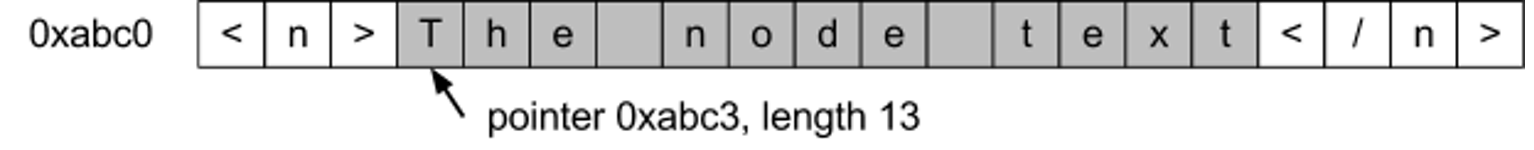
\includegraphics{pugixml-images/image01.png}
\caption{An example of basic in-place text parsing.}
\end{figure}

Most in-place parsers have to deal with additional issues. In the case
of pugixml, there are two: simplifying string access and transforming
XML data during parsing.

Accessing strings that are parsed in-place is difficult because they are
not null-terminated. That is, the character after the string is not a
null byte, but is instead the next character in the XML document, such
as an open angle bracket (\texttt{\textless{}}). This makes it difficult
to use standard C/C++ string functions that expect null-terminated
strings.

To make sure we can use these functions we'll have to null-terminate the
strings during parsing. Since we can't easily insert new characters, the
character after the last character of each string will have to be
overwritten with a null character. Fortunately, we can always do this in
XML: a character that follows the end of a string is always a markup
character and is never relevant to document representation in memory.

\begin{figure}[htbp]
\centering
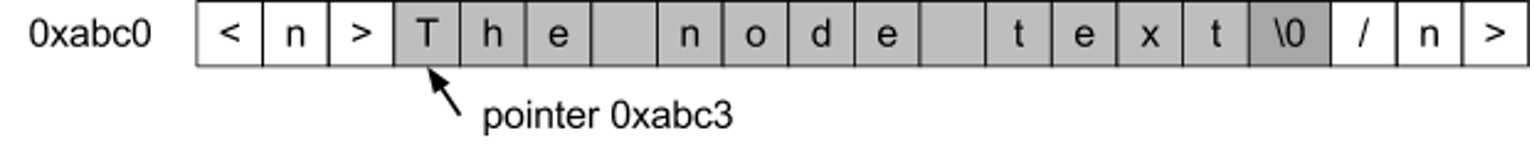
\includegraphics{pugixml-images/image03.png}
\caption{Adjusting in-place parsing for null-terminated strings.}
\end{figure}

The second issue is more complicated: often the string value and the
representation in the XML file are different. A conforming parser is
expected to perform decoding of the representation. Since doing this
during node object access would make object access performance
unpredictable, we prefer to do this at parsing time. Depending on the
content type, an XML parser could be required to perform the following
transformations:

\begin{aosaitemize}
\item
  End-of-line handling: The input document can contain various types of
  line endings and the parser should normalize them as follows: any
  two-character sequence of one carriage return (ASCII 0xD) and one line
  feed (ASCII 0xA) and any free-standing carriage return should be
  replaced with a line feed character. For example, the line

\begin{verbatim}
  `line1\xD\xAline2\xDline3\xA\xA`
\end{verbatim}

  should be transformed to

\begin{verbatim}
  `line1\xAline2\xAline3\xA\xA`.
\end{verbatim}
\item
  Character reference expansion: XML supports escaping characters using
  their Unicode code point with either decimal or hexadecimal
  representation. For example, \texttt{\&\#97;} should expand to
  \texttt{a} and \texttt{\&\#xf8;} should expand to ø.
\item
  Entity reference expansion: XML supports generic entity references,
  where \&name; is replaced with the value of entity name. There are
  five predefined entities: \texttt{\&lt;} (\textless{}), \texttt{\&gt;}
  (\textgreater{}), \texttt{\&quot;} (``), \texttt{\&apos;} (') and
  \texttt{\&amp;} (\&).
\item
  Attribute-value normalization: in addition to expanding references,
  the parser should perform whitespace normalization when parsing
  attribute values. All whitespace characters (space, tab, carriage
  return and line feed) should be replaced with a space. Additionally,
  depending on the type of the attribute, leading and trailing
  whitespaces should be removed and whitespace sequences in the middle
  of the string should be collapsed into a single space.
\end{aosaitemize}

It is possible to support an arbitrary transformation in an in-place
parser by modifying the string contents, given an important constraint:
a transformation must never increase the length of the string. If it
does, the result might overlap with significant data in the document.
Fortunately, all of the above transformations satisfy this
requirement.\footnote{This is obvious for all transformations, except
  perhaps Unicode transformation. In that case, both UTF-8 and UTF-16
  encodings are more compact than hexadecimal or decimal representation
  of Unicode code points, which is why replacing one with the other
  never increases the length.}

General entity expansion does \emph{not} satisfy this constraint. Since
pugixml does not support \texttt{DOCTYPE} declarations, and it is
impossible to specify custom entities without \texttt{DOCTYPE}, any
supported document can be fully parsed using in-place parsing.\footnote{It
  is possible to support general entity references with in-place parsing
  by splitting every string with an entity reference into three nodes:
  prefix string before entity reference, a node of a special type that
  contains the reference id, and a suffix string, which may have to be
  split further. This approach is used by the Microsoft XML parser (for
  different reasons).}

\begin{figure}[htbp]
\centering
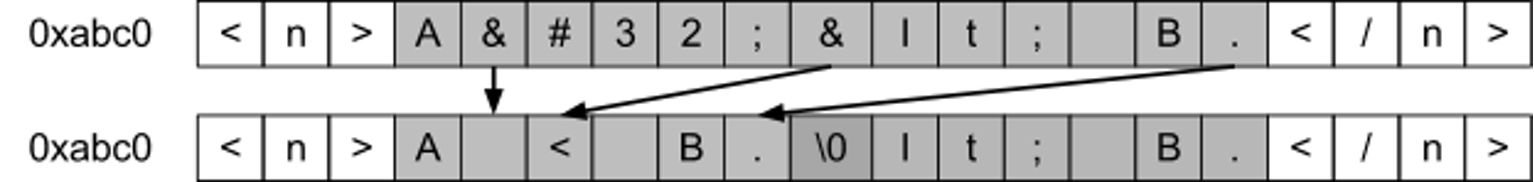
\includegraphics{pugixml-images/image04.png}
\caption{Text transformations with in-place text parsing.}
\end{figure}

Interestingly, in-place parsing can be used with memory-mapped file
I/O.\footnote{See \url{http://en.wikipedia.org/wiki/Memory-mapped_file}.}
Supporting null-termination and text transformation requires a special
memory mapping mode known as \emph{copy-on-write} to avoid modifying the
file on disk.

Using memory mapped file I/O with in-place parsing has the following
benefits:

\begin{aosaitemize}

\item
  The kernel can usually map cache pages directly into the process
  address space, thus eliminating a memory copy that would have happened
  with standard file I/O.
\item
  If the file is not already in the cache, the kernel can prefetch
  sections of the file from disk, effectively making I/O and parsing
  parallel.
\item
  Since only modified pages need to allocate physical memory, memory
  consumption can be greatly decreased on documents with large text
  sections.
\end{aosaitemize}

\aosasectii{Optimizing character-wise operations}

Eliminating string copies is not the only thing we can do to optimize
parser performance. When comparing parser performance, a useful metric
is the average number of processor cycles spent for each character.
While this varies among documents and processor architectures, it is
reasonably stable for documents of similar structure. Thus it makes
sense to optimize for this metric, and an obvious place to start is in
the operations performed for each character.

The most important operation is detecting character set membership:
given a character from the input stream, does it belong to a certain set
of characters?

A useful approach is to create a Boolean flag table, where for each
character value a true/false value is stored depending on whether the
character belongs to the set or not. Depending on the encoding,
different table data structures and sizes make sense as follows:

\begin{aosaitemize}
\item
  For encodings where each character occupies no more than 8 bits, a
  table of size 256 is sufficient.
\item
  For UTF-8, we would like to use a byte-indexed table to avoid code
  point decoding; this works only if all characters with code points
  (i.e.~numeric values) above 127 belong to the set or no characters
  with code points above 127 belong to the set. If either of these are
  true, then a table of size 256 is sufficient. The first 128 entries of
  the table are filled with true or false (depending on whether the
  character is in the target set) and the last 128 entries of the table
  all share the same value. Because of the way UTF-8 encodes data, all
  code points above 127 will be represented as sequences of bytes with
  values above 127. Furthermore, the first character of the sequence
  will also be above 127.
\item
  For UTF-16 or UTF-32, tables of large sizes are usually impractical.
  Given the same constraint as the one for optimized UTF-8, we can leave
  the table to be 128 or 256 entries large, and add an additional
  comparison to deal with values outside the range.
\end{aosaitemize}

Note that we only need one bit to store the true/false value, so it
might make sense to use bitmasks to store eight different character sets
in one 256 byte table. Pugixml uses this approach to save cache space:
on the x86 architecture, checking a boolean value usually has the same
cost as checking a bit within a byte, provided that bit position is a
compile-time constant. This C code demonstrates this approach:

\begin{verbatim}
enum chartype_t {
  ct_parse_pcdata  = 1, // \0, &, \\r, \<
  ct_parse_attr    = 2, // \0, &, \\r, ', "
  ct_parse_attr_ws = 4, // \0, &, \\r, ', ", \\n, tab
  // ...
};
static const unsigned char table[256] = {
  55, 0, 0, 0, 0, 0, 0, 0, 0, 12, 12, 0, 0, 63, 0, 0, // 0-15
  // ...
};
bool ischartype_utf8(char c, chartype_t ct) {
  // note: unsigned cast is important to
  // guarantee that the value is in 0..255 range
  return ct & table[(unsigned char)c];
}

bool ischartype_utf16_32(wchar_t c, chartype_t ct) {
  // note: unsigned cast is important to
  // guarantee that the value is not negative
  return ct & ((unsigned)c < 128 ? table[(unsigned)c] : table[128]);
}
\end{verbatim}

If the tested range includes all characters in a certain interval, it
might make sense to use a comparison instead of a table lookup. With
careful use of unsigned arithmetics just one comparison is needed. For
example, a test for a character being a digit:

\begin{verbatim}
bool isdigit(char ch) { return (ch >= '0' && ch <= '9'); }
\end{verbatim}

\noindent can be rewritten using just one comparison:

\begin{verbatim}
bool isdigit(char ch) { return (unsigned)(ch - '0') < 10; }
\end{verbatim}

If we work character by character, improving on the above approaches is
usually impossible. However, it is sometimes possible to work on groups
of characters and use vectorized checks. If the target system has some
form of SIMD instructions available, you can usually use these
instructions for fast operation on groups of 16 characters or more.

Even without resorting to platform-specific instruction sets it is
sometimes possible to vectorize character operations. For example, here
is one way to check if four consecutive bytes in a UTF-8 byte stream
represent ASCII symbols\footnote{Of course, the data has to be suitably
  aligned for this to work; additionally, this technique violates strict
  aliasing rules of the C/C++ standard, which may or may not be a
  problem in practice.

  (\emph{(const uint32\_t})data \& 0x80808080) == 0}:

Finally, whatever you do, avoid \texttt{is.*()} functions from the
standard library (such as \texttt{isalpha()}) for performance-sensitive
code. Even the best implementations check whether the current locale is
``C'', which is more expensive than the table lookup itself, and the
worst implementations can be two orders of magnitude slower than
that.\footnote{See \aosachapref{s:khmer} for another example of this
  problem.}

\aosasectii{Optimizing string transformations}

In pugixml, the reading and transformation of values is particularly
time-consuming. For example, let's look at reading plain-character data
(PCDATA); e.g., the text between the XML tags. Any standard conforming
parser, as previously discussed, should perform reference expansion and
end of line normalization during PCDATA content processing.\footnote{Pugixml
  allows the user to turn either of these off at runtime for both
  performance and data preservation reasons. For example, you might be
  dealing with documents where it is important to preserve the exact
  type of newline sequences, or where entity references should be left
  unexpanded by the XML parser in order to be processed afterwards.}

For example, the following text in XML:

\begin{verbatim}
A&#32;&lt; B.
\end{verbatim}

\noindent should be transformed to

\begin{verbatim}
A < B.
\end{verbatim}

The PCDATA parsing function takes a pointer to the start of PCDATA
value, and proceeds by reading the rest of the value, converting the
value data in-place and null-terminating the result.

Since there are two boolean flags, we have four variations of this
function. In order to avoid expensive run-time checks, we're using
boolean template arguments for these flags---thus we're compiling four
variations of a function from a single template, and then using runtime
dispatch to obtain the correct function pointer once before the parsing
begins. The parser calls the function using this function pointer.

This allows the compiler to remove condition checks for flags and remove
dead code for each specialization of the function. Importantly, inside
the function's parsing loop we use a fast character set test to skip all
characters that are part of the usual PCDATA content, and only process
the characters we're interested in. Here's what the code looks like:

\begin{verbatim}
template <bool opt_eol, bool opt_escape> struct
strconv_pcdata_impl {
  static char_t* parse(char_t* s) {
    gap g;
    while (true) {
      while (!PUGI__IS_CHARTYPE(*s, ct_parse_pcdata)) ++s;
      if (*s == '<') { // PCDATA ends here
        *g.flush(s) = 0;
        return s + 1;
      } else if (opt_eol && *s == '\r') { // 0x0d or 0x0d 0x0a pair
        *s++ = '\n'; // replace first one with 0x0a
        if (*s == '\n') g.push(s, 1);
      } else if (opt_escape && *s == '&') {
        s = strconv_escape(s, g);
      } else if (*s == 0) {
        return s;
      } else {
        ++s;
      }
    }
  }
};
\end{verbatim}

\noindent An additional function gets a pointer to a suitable
implementation based on runtime flags; e.g.,
\texttt{\&strconv\_pcdata\_impl\textless{}false, true\textgreater{}::parse}.

One unusual item in this code is the \texttt{gap} class instance. As
shown before, if we do string transformations, the resulting string
becomes shorter because some of the characters have to be removed. There
are several ways of doing this.

One strategy (that pugixml \emph{doesn't} use) is to keep separate
\texttt{read} and \texttt{write} pointers that both point to the same
buffer. In this case the \texttt{read} pointer tracks the current read
position, and the \texttt{write} pointer tracks the current write
position. At all times the invariant \texttt{write \textless{}= read}
should hold. Any character that has to be a part of the resulting string
must be explicitly written to the write pointer. This technique avoids
the quadratic cost of naive character removal, but is still inefficient,
since we now read and write all characters in the string every time,
even if we don't need to modify the string.

An obvious extension of this idea is to skip the prefix of the original
string that does not need to be modified and only start writing
characters after that prefix---indeed, that's how algorithms like the
one behind \texttt{std::remove\_if()} commonly operate.

Pugixml follows a different approach (see
\aosafigref{posa.pugixml.gapops}). At any time there is \emph{at most
one gap} in the string. The gap is a sequence of characters that are no
longer valid because they are no longer part of the final string. When a
new gap has to be added because another substitution was made (e.g.,
replacing \texttt{\&quot;} with " generates a gap of 5 characters), the
existing gap (if one exists) is collapsed by moving the data between two
gaps to the beginning of the first gap and then remembering the new gap.
In terms of complexity, this approach is equivalent to the approach with
read and write pointers; however it allows us to use faster routines to
collapse gaps. (Pugixml uses memmove which can copy more efficiently
compared to a character-wise loop, depending on the gap length and on C
runtime implementation.)

\aosafigure{pugixml-images/image02.png}{An example of gap operations during PCDATA conversion.}{posa.pugixml.gapops}

\aosasectii{Optimizing control flow}

The pugixml parser itself can be thought of as a recursive-descent
parser. However, the recursion is transformed into a loop to improve
performance. A node cursor acts as a stack. When a start tag is
encountered, a new node is appended to the cursor and becomes the new
cursor; when an end tag is encountered, the cursor is moved to the
parent of the current cursor. This makes stack space consumption
constant regardless of the input document, which improves robustness,
and avoids potentially expensive function calls.

The parser uses a dispatch loop that reads a character from the stream,
reads zero or more characters past that (depending on the first
character) to determine the tag type, and then proceeds to the code that
parses the relevant tag. For example, if the first character is
\texttt{\textless{}}, we have to read at least one more character to
differentiate between a start tag, end tag, comment, or other types of
tags. Pugixml also uses \texttt{goto} statements to avoid going through
the dispatch loop in certain cases --- for example, text content parsing
stops at the end of stream or the \texttt{\textless{}} character.
However, if the next character is \texttt{\textless{}}, we don't have to
go through the dispatch loop only to read the character again and check
that it's \texttt{\textless{}}; we can jump straight to the code that
does the tag parsing.

Two important optimizations for such code are branch ordering and code
locality.

In the parser, various parts of the code handle various forms of inputs.
Some of them (such as tag name or attribute parsing) execute frequently,
while others (such as DOCTYPE parsing) rarely execute at all. Even
within a small section of code, different inputs have different
probabilities. For example, after the parser encounters an open angle
bracket (\texttt{\textless{}}), the most likely character to appear next
is a character of a tag name. Next most likely is \texttt{/}\footnote{The
  reason \texttt{/} is less probable than a tag name character is that
  for every end tag there is a start tag, but there are also
  empty-element tags such as \texttt{\textless{}node/\textgreater{}}.},
followed by \texttt{!} and \texttt{?}.

With this in mind, it is possible to rearrange the code to yield faster
execution. First, all ``cold'' code; that is, code that is unlikely to
ever execute, or is unlikely to execute frequently---in the case of
pugixml this includes all XML content except element tags with
attributes and text content --- has to be moved out of the parser loop
into separate functions. Depending on the function's contents and the
compiler, adding attributes such as \texttt{noinline}, or specifically
marking extra functions as ``cold'' might help. The idea is to limit the
amount of code inlined into the main parser function to the hot code.
This helps the compiler optimize the function by keeping the control
flow graphs small, and keeps all hot code as close together as possible
to minimize instruction cache misses.

After this, in both hot and cold code it makes sense to order any
conditional chains you have by condition probability. For example, code
like this is not efficient for typical XML content:

\begin{verbatim}
if (data[0] == '<')
{
  if (data[1] == '!') { ... }
  else if (data[1] == '/') { ... }
  else if (data[1] == '?') { ... }
  else { /* start-tag or unrecognized tag */ }
}
\end{verbatim}

\noindent A better version would look like this:

\begin{verbatim}
if (data[0] == '<')
{
  if (PUGI__IS_CHARTYPE(data[1], ct_start_symbol)) { /* start-tag */ }
    else if (data[1] == '/') { ... }
    else if (data[1] == '!') { ... }
    else if (data[1] == '?') { ... }
    else { /* unrecognized tag */ }
}
\end{verbatim}

\noindent In this version the branches are sorted by probability from
most-frequent to least-frequent. This minimizes the average amount of
condition tests and conditional jumps performed.

\aosasectii{Ensuring memory safety}

Memory safety is an important concern for a parser. On any input
(including malformed input), the parser must never read or write memory
beyond the end of the input buffer. There are two ways to implement
this. The first option is to make sure the parser checks the current
read position against the end position everywhere. The second option is
to use a null-terminated string as an input and make sure the parser
handles the null terminator accordingly. Pugixml uses an extended
variant of the latter.

Additional read position checks incur a noticeable performance overhead,
whereas the null terminator is often naturally included in existing
checks. For example, the loop

\begin{verbatim}
while (PUGI__IS_CHARTYPE(*s, ct_alpha))
  ++s;
\end{verbatim}

\noindent skips a run of alphabetical characters and stops at the null
terminator or the next non-alphabetic character without requiring extra
checks. Storing the buffer end position everywhere also reduces the
overall speed because it usually requires an extra register. Function
calls also get more expensive since you need to pass two pointers
(current position and end position) instead of one.

However, requiring null-terminated input is less convenient for library
users: often XML data gets read into a buffer that might not have space
for an extra null terminator. From the client's point of view a memory
buffer should be a pointer and a size with no null terminator.

Since the internal memory buffer has to be mutable for in-place parsing
to work, pugixml solves this problem in a simple way. Before parsing, it
replaces the last character in the buffer with a null terminator and
keeps track of the value of the old character. That way, the only places
it has to account for the value of the last character are places where
it is valid for the document to end. For XML, there are not
many\footnote{For example, if a tag name scan stopped at the null
  terminator, then the document is invalid because there are no valid
  XML documents where the character before the last one is a part of tag
  name.}, so the approach results in a net win.\footnote{Of course, the
  parsing code becomes more complicated, since some comparisons need to
  account for the value of the last character, and all others need to
  skip it for performance reasons. A unit test suite with good coverage
  and fuzz testing helps keep the parser correct for all document
  inputs.}

This summarizes the most interesting tricks and design decisions that
help keep pugixml parser fast for a wide range of documents. However,
there is one last performance-sensitive component of the parser that is
worth discussing.

\aosasecti{Data structures for the document object model}

An XML document is a tree-like structure. It contains one or more nodes;
each node can contain one or more nodes; nodes can represent different
types of XML data, such as elements or text; and element nodes can also
contain one or more attributes.

Every representation of node data is usually a tradeoff between memory
consumption and the performance of various operations. For example,
\emph{semantically} a node contains a collection of child nodes; this
collection can be represented in the data structure. Specifically, this
data can be stored as an array or as a linked list. An array
representation would allow for fast index-based access; a linked list
representation would allow for constant-time insertions or
removals.\footnote{Tree modification is important---while there are ways
  to represent immutable trees much more efficiently compared to what
  pugixml is doing, tree mutation is a much needed feature both for
  constructing documents from scratch and for modifying existing
  documents.}

Pugixml chooses to represent both node and attribute collections as a
linked list. Why not as arrays? The two main benefits of arrays are fast
index-based access (which is not particularly important for pugixml) and
memory locality (which can be achieved through different means).

Fast index-based access is usually not needed because the code that
processes the XML tree either needs to iterate through all child nodes
or get a specific node that is identified by the value of an attribute
(e.g. ``get the child node with an `id' attribute equal to
`X'\,'').\footnote{More complex logic can be used as well.} Index-based
access is also fragile in a mutable XML document: for example, adding
XML comments alters the indices of subsequent nodes in the same subtree.

Memory locality depends on the allocation algorithm. With the right
algorithm, linked lists can be as efficient as arrays if list nodes are
allocated sequentially. (More on this later.)

The basic tree data structure with children stored in an array (which is
\emph{not} what pugixml uses) usually looks like this:\footnote{The
  capacity field is required to implement an amortized constant-time
  addition. See \mbox{\url{http://en.wikipedia.org/wiki/Dynamic_array}}
  for more information.

  struct Node \{ Node* children; size\_t children\_size; size\_t
  children\_capacity; \};}

The basic tree data structure that uses linked lists (which is not
\emph{exactly} what pugixml uses) looks like this:

\begin{verbatim}
struct Node {
  Node* first_child;
  Node* last_child;
  Node* prev_sibling;
  Node* next_sibling;
};
\end{verbatim}

Here, the \texttt{last\_child} pointer is necessary to support backwards
iteration and appending in O(1) time.

Note that with this design it is easy to support different node types to
reduce memory consumption; for example, an element node needs an
attribute list but a text node does not. The array approach forces us to
keep the size of all node types the same, which prevents such
optimization from being effective.

Pugixml uses a linked list-based approach. That way, node modification
is always O(1). Furthermore, the array approach would force us to
allocate blocks of varying sizes, ranging from tens of bytes to
megabytes in case of a single node with a lot of children; whereas in
the linked list approach there are only a few different allocation sizes
needed for node structure. Designing a fast allocator for fixed size
allocations is usually easier than designing a fast allocator for
arbitrary allocations which is another reason pugixml chooses this
strategy.

To keep memory consumption closer to the array-based approach, pugixml
omits the \texttt{last\_child} pointer, but keeps access to the last
child available in O(1) time by making the sibling list partially cyclic
with \texttt{prev\_sibling\_cyclic}:

\begin{verbatim}
struct Node {
  Node* first_child;
  Node* prev_sibling_cyclic;
  Node* next_sibling;
};
\end{verbatim}

\noindent This data structure is organized as follows:

\begin{aosaenumerate}
\def\labelenumi{\arabic{enumi}.}

\item
  \texttt{first\_child} points to the first child of the node, or
  \texttt{NULL} if node has no children.
\item
  \texttt{prev\_sibling\_cyclic} points to the left sibling of the node
  (a child of node's parent that is immediately before the node in the
  document). If the node is the leftmost one (i.e., if the node is the
  first child of its parent), \texttt{prev\_sibling\_cyclic} points to
  the last child of the node's parent, or to itself if it is the only
  child. \texttt{prev\_sibling\_cyclic} cannot be \texttt{NULL}.
\item
  \texttt{next\_sibling} points to the right sibling of the node or
  \texttt{NULL} if the node is the last child of its parent.
\end{aosaenumerate}

\begin{figure}[htbp]
\centering
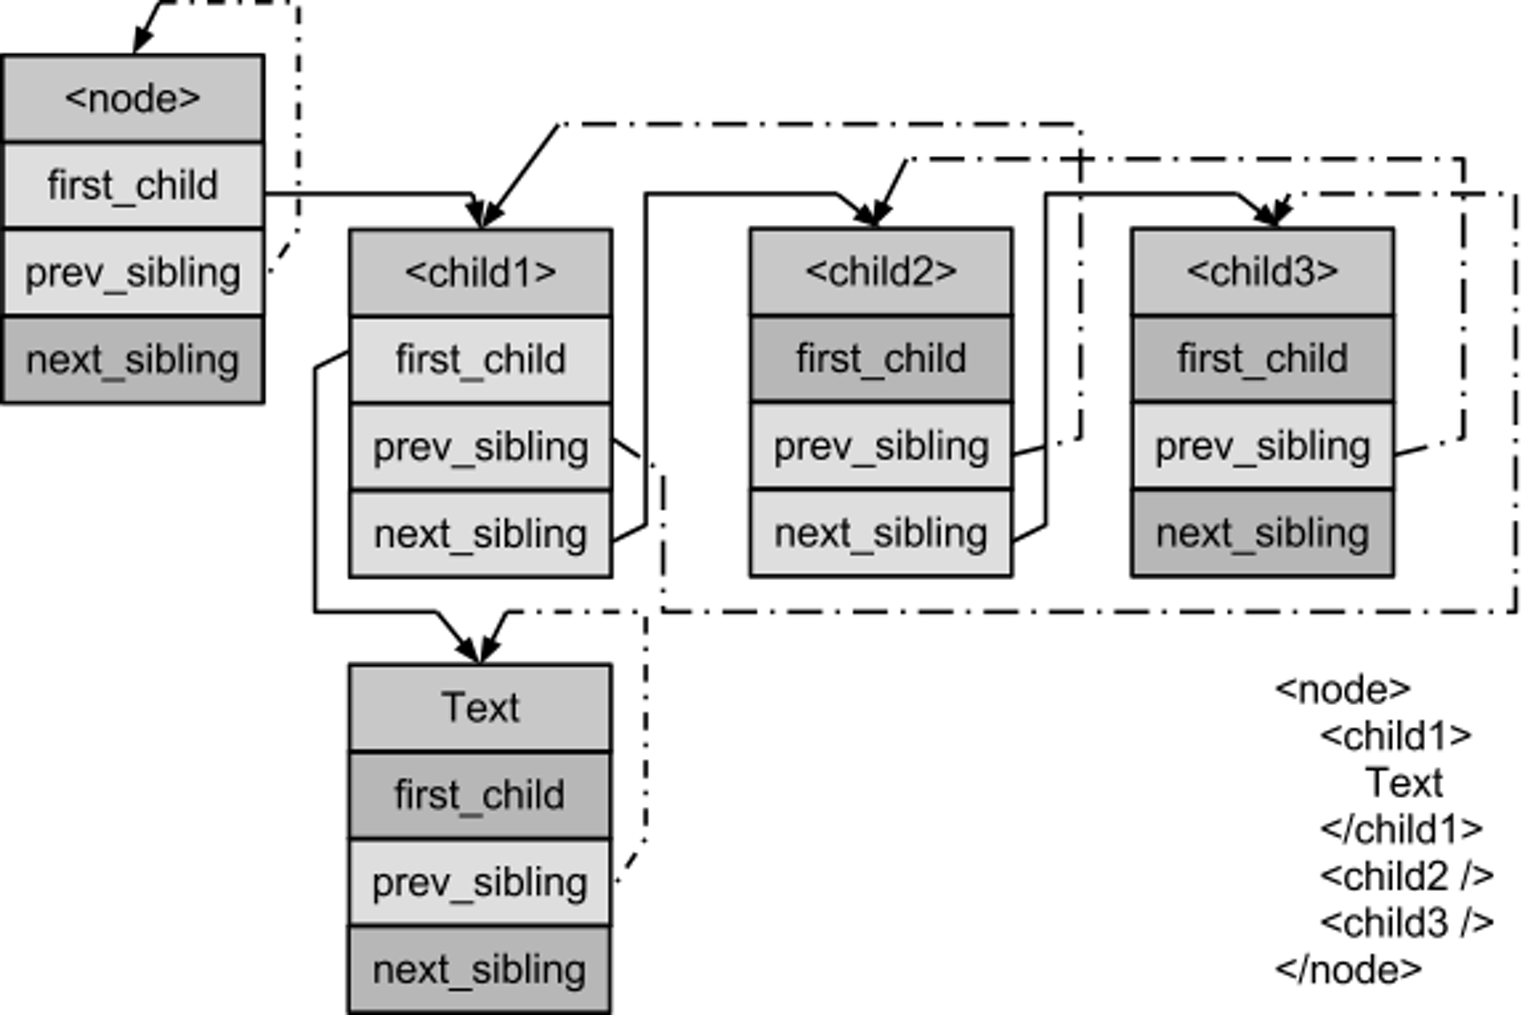
\includegraphics{pugixml-images/image00.png}
\caption{An example subtree, represented using partially-cyclic linked
lists.}
\end{figure}

\noindent With this structure, all of the following operations are
constant-time:

\begin{verbatim}
Node* last_child(Node* node) {
  return (node->first_child) ?
      node->first_child->prev_sibling_cyclic : NULL;
}

Node* prev_sibling(Node* node) {
  return (node->prev_sibling_cyclic->next_sibling) ?
      node->prev_sibling_cyclic : NULL;
}
\end{verbatim}

The array-based approach and the linked list approach with the
partially-cyclic-sibling-list trick become equivalent in terms of memory
consumption. Using 32-bit types for size/capacity makes the array-based
node smaller on 64-bit systems.\footnote{This assumes a limit of $2^{32}$
  child nodes.} In the case of pugixml, other benefits of linked lists
outweigh the costs.

With the data structures in place, it is time to talk about the last
piece of the puzzle---the memory allocation algorithm.

\aosasecti{Stack-based memory allocation}

A fast memory allocator is critical for the performance of a DOM parser.
In-place parsing eliminates allocation for string data, but DOM nodes
still need to be allocated. String allocations of varying sizes are also
needed to support tree mutation. Preserving allocation locality is
important for tree traversal performance: if successive allocation
requests return adjacent memory blocks, it becomes easy to ensure tree
locality during construction. Finally, destruction speed is important:
in addition to deletion in constant time, the ability to quickly
deallocate all memory allocated for the document without deleting each
node individually can significantly improve the time it takes to destroy
large documents.

Before discussing the allocation scheme that pugixml uses, let's discuss
a scheme that it \emph{could} have used.

Since DOM nodes have a small set of required allocation sizes, it would
be possible to use a standard memory pool based on free lists for each
size. For such a pool, there would be a single linked list of free
blocks where each block is the same size. During an allocation request,
if the free list is empty, a new page with an array of blocks is
allocated. The blocks are linked together to form a single linked list,
which then becomes the free list of the allocator. If a free list is not
empty, the first block is removed from the list and returned to the
user. A deallocation request simply prepends the block to the free list.

This allocation scheme is very good at reusing memory---allocating a
node after freeing some other node would reuse the memory immediately.
However, adding support for releasing memory pages back to the heap
requires additional per-page tracking of used blocks. The locality of
the allocations also varies on the prior usage of the allocator, which
may end up decreasing traversal performance.

Since pugixml supports tree mutation, it requires support for
allocations of arbitrary size. It was unclear whether this allocator
could be easily extended to support arbitrarily sized allocations and
other required features of pugixml without impacting the parsing
performance. Employing a complicated general-purpose allocation scheme
akin to the algorithms implemented in dlmalloc and other general-purpose
memory allocators was also not an option---such allocators tend to be
somewhat slower than simple free lists, not to mention more complex.
Pugixml needed something simple and fast.

It turns out that the simplest allocation scheme possible is the stack
allocator. This allocator works as follows: given a memory buffer and an
offset inside that buffer, an allocation only requires increasing that
offset by the allocation size. Of course, it is impossible to predict
the memory buffer size in advance, so an allocator has to be able to
allocate new buffers on demand.

This code illustrates the general idea:

\begin{verbatim}
const size_t allocator_page_size = 32768;
struct allocator_page {
  allocator_page* next_page;
  size_t offset;
  char data[allocator_page_size];
};
struct allocator_state {
  allocator_page* current;
};

void* allocate_new_page_data(size_t size) {
  size_t extra_size = (size > allocator_page_size) ?
    size - allocator_page_size : 0;
  return malloc(sizeof(allocator_page) + extra_size);
}

void* allocate_oob(allocator_state* state, size_t size) {
  allocator_page* page = (allocator_page*)allocate_new_page_data(size);
  // add page to page list
  page->next_page = state->current;
  state->current = page;
  // user data is located at the beginning of the page
  page->offset = size;
  return page->data;
}

void* allocate(allocator_state* state, size_t size) {
  if (state->current->offset + size <= allocator_page_size) {
    void* result = state->current->data + state->current->offset;
    state->current->offset += size;
    return result;
  }
  return allocate_oob(state, size);
}
\end{verbatim}

Supporting allocations that are larger than page size is easy. We just
allocate a larger memory block, but treat it in the same way as we would
treat a small page.\footnote{For performance reasons this implementation
  does not adjust the offset to be aligned. Instead it expects that all
  stored types need pointer type alignment, and that all allocation
  requests specify size aligned to a pointer size.}

This allocator is very fast. It's probably the fastest allocator
possible, given the constraints. Benchmarks show it to be faster than a
free list allocator, which has to do more work to determine the correct
list based on page size and has to link all blocks in a page together.
Our allocator also exhibits almost perfect memory locality. The only
case where successive allocations are not adjacent is when it allocates
a new page.

In case of small allocations this allocator does not waste memory.
However, it is possible to devise a hypothetical memory allocation
pattern (that might arise in practice) where it does waste memory. A
sequence of allocation sizes alternating between 64 and 65536 would
cause a new page allocation on every call, resulting in 30\% wasted
space. For this reason, the implementation of this allocator in pugixml
behaves slightly differently: if an allocation is larger than a quarter
of the default page size, it allocates an entire page for it, and
instead of adding it to the front of the page list, it adds it after the
first entry. That way, the small allocations that happen after a large
one still go into the page in progress.

Note that \texttt{allocate\_oob()} is ``cold'' code---that is, it only
gets executed once we exhaust the current page, which should be a rare
event. For this reason, explicitly forbidding the compiler to inline it
can improve performance.\footnote{This improvement is measurable in
  pugixml.} This also means that having more complicated logic in
\texttt{allocate\_oob()}---for example, logic that treats large
allocations differently---does not have any effect on the overall
performance of the allocator.

Finally, since all allocations are contained in some page and the
allocator keeps the entire page list as a state, it's very easy to
destroy the entire page list and thereby free all allocated memory. This
is very fast since it only touches headers of each page in memory.

\aosasecti{Supporting deallocation in a stack-based allocator}

The implementation discussed in the previous section does not have any
way to release or reuse memory.

Interestingly, for a lot of use cases this is actually not a big deal.
Since we can release the memory on document destruction by removing all
pages\footnote{This, of course, means that nodes or attributes cannot
  exist without the document---which, in C++, is a reasonable design
  decision for node ownership.}, parsing a document or creating a new
document does not consume extra memory. However, a problem arises when
we delete a substantial portion of the document and then proceed to add
more nodes to the document. Since we never reuse memory, peak memory
consumption can become very significant.

Implementing fine-grained reuse while preserving the allocation
performance seems impossible. However, a compromise can be reached.
During allocation, we'll count the number of allocations made in each
respective page. Deallocation requests then have to get a reference to
the page of the destroyed pointer and decrease this counter. If this
counter reaches zero, the page is not needed any more and can be
removed.

For this to be possible, we need to know what page each object was
allocated in. This is possible without storing a pointer to the page,
but it is difficult.\footnote{It is possible to do this without storing
  extra data using a page alignment that is larger than the page size
  (i.e., allocate all pages using a 64k allocations with 64k alignment),
  but it is not possible to use large allocation alignments in a
  portable way without huge memory overhead.} For this reason, pugixml
resorts to storing a page pointer alongside each allocation.

Pugixml uses two different approaches to reducing the memory overhead
associated with storing a page pointer with each allocation.

The first approach is to store a page pointer in a single pointer-sized
field with several bits of unrelated data which we would have to store
anyway. The allocator makes sure that all pages are aligned to 32 bytes,
so this means that the five least significant bits of every page pointer
are zero; as such they can be used to store arbitrary data. Five bits is
a good number because the metadata of an XML node fits: three bits are
used for a node type, and two bits are used to specify whether the
node's name and value reside in the in-place buffer.

The second approach is to store the offset of the allocated element
relative to the beginning of the page, which allows us to get the
address of the page pointer in the following way:

\begin{verbatim}
(allocator_page*)((char*)(object) -
    object->offset - offsetof(allocator_page, data))
\end{verbatim}

\noindent If our page size is limited by $2^{16} = 65536$ bytes, this
offset fits in 16 bits, so we can spend 2 bytes instead of 4 storing it.
Pugixml uses this approach for heap-allocated strings.

An interesting feature of the resulting algorithm is that it respects
the locality of reference exhibited by the code that uses the allocator.
Locality of allocation requests eventually leads to locality of
allocated data in space. Locality of \emph{deallocation} requests in
space leads to successfully released memory. This means, in the case of
tree storage, that deletion of a large subtree usually releases most of
the memory that is used by the subtree.

Of course, for certain usage patterns nothing is ever deleted until the
entire document is destroyed. For example, if a page size is 32000
bytes, we can do one million 32-byte allocations, thus allocating 1000
pages. If we keep every 1000th object alive and delete the remaining
objects, each page will have exactly one object left, which means that,
although the cumulative size of live objects is now
$1000 \cdot 32 = 32000$ bytes, we still keep all pages in memory
(consuming 32 million bytes). This results in an extremely high memory
overhead. However, such usage is extremely unlikely, and the benefits of
the algorithm outweigh this problem for pugixml.

\aosasecti{Conclusion}

Optimizing software is hard. In order to be successful, optimization
efforts almost always involve a combination of low-level
micro-optimizations, high-level performance-oriented design decisions,
careful algorithm selection and tuning, balancing among memory,
performance, implementation complexity, and more. Pugixml is an example
of a library that needs all of these approaches to deliver a very fast
production-ready XML parser---even though compromises had to be made to
achieve this. A lot of the implementation details can be adapted to
different projects and tasks, be it another parsing library or something
else entirely. The author hopes that the presented tricks were
entertaining and that some of them will be useful for other projects.

\end{aosachapter}


\begin{aosachapter}{MemShrink}{s:memshrink}{Kyle Huey}

\aosasecti{Introduction}

Firefox has long had a reputation for using too much memory. The
accuracy of that reputation has varied over the years but it has stuck
with the browser. Every Firefox release in the past several years has
been met by skeptical users with the question ``Did they fix the memory
leak yet?'' We shipped Firefox 4 in March 2011 after a lengthy beta
cycle and several missed ship dates---and it was met by the same
questions. While Firefox 4 was a significant step forward for the web in
areas such as open video, JavaScript performance, and accelerated
graphics, it was unfortunately a significant step backwards in memory
usage.

The web browser space has become very competitive in recent years. With
the rise of mobile devices, the release of Google Chrome, and Microsoft
reinvesting in the web, Firefox has found itself having to contend with
a number of excellent and well-funded competitors instead of just a
moribund Internet Explorer. Google Chrome in particular has gone to
great lengths to provide a fast and slim browsing experience. We began
to learn the hard way that being a good browser was no longer good
enough; we needed to be an excellent browser. As Mike Shaver, at the
time VP of Engineering at Mozilla and a longtime Mozilla contributor,
said, ``this is the world we wanted, and this is the world we made.''

That is where we found ourselves in early 2011. Firefox's market share
was flat or declining while Google Chrome was enjoying a fast rise to
prominence. Although we had begun to close the gap on performance, we
were still at a significant competitive disadvantage on memory
consumption as Firefox 4 invested in faster JavaScript and accelerated
graphics often at the cost of increased memory consumption. After
Firefox 4 shipped, a group of engineers led by Nicholas Nethercote
started the MemShrink project to get memory consumption under control.
Today, nearly a year and a half later, that concerted effort has
radically altered Firefox's memory consumption and reputation. The
``memory leak'' is a thing of the past in most users' minds, and Firefox
often comes in as one of the slimmest browsers in comparisons. In this
chapter we will explore the efforts we made to improve Firefox's memory
usage and the lessons we learned along the way.

\aosasecti{Architecture Overview}

You will need a basic grasp of what Firefox does and how it works to
make sense of the problems we encountered and the solutions we found.

A modern web browser is fundamentally a virtual machine for running
untrusted code. This code is some combination of HTML, CSS, and
JavaScript (JS) provided by third parties. There is also code from
Firefox add-ons and plugins. The virtual machine provides capabilities
for computation, layout and styling of text, images, network access,
offline storage, and even access to hardware-accelerated graphics. Some
of these capabilities are provided through APIs designed for the task at
hand; many others are available through APIs that have been repurposed
for entirely new uses. Because of the way the web has evolved, web
browsers must be very liberal in what they accept, and what browsers
were designed to handle 15 years ago may no longer be relevant to
providing a high-performance experience today.

Firefox is powered by the Gecko layout engine and the Spidermonkey JS
engine. Both are primarily developed for Firefox, but are separate and
independently reusable pieces of code. Like all widely used layout and
JS engines, both are written in C++. Spidermonkey implements the JS
virtual machine including garbage collection and multiple flavors of
just-in-time compilation (JIT). Gecko implements most APIs visible to a
web page including the DOM, graphical rendering via software or hardware
pipelines, page and text layout, a full networking stack, and much more.
Together they provide the platform that Firefox is built on. The Firefox
user interface, including the address bar and navigation buttons, is
just a series of special web pages that run with enhanced privileges.
These privileges allow them access to all sorts of features that normal
web pages cannot see. We call these special, built-in, privileged pages
\emph{chrome} (no relation to Google Chrome) as opposed to
\emph{content}, or normal web pages.

For our purposes, the most interesting details about Spidermonkey and
Gecko are how they manage memory. We can categorize memory in the
browser based on two characteristics: how it is allocated and how it is
freed. Dynamically allocated memory (the \emph{heap}) is obtained in
large chunks from the operating system and divided into requested
quantities by the heap allocator. There are two main heap allocators:
the specialized garbage-collected heap allocator used for the
garbage-collected memory (the \emph{GC heap}) in Spidermonkey, and
jemalloc, which is used by everything else in Spidermonkey and Gecko.
There are also three methods of freeing memory: manually, via reference
counting, and via garbage collection.

\aosafigure{memshrink-images/figure1.png}{Memory management in Firefox}{memshrink}

The GC heap in Spidermonkey contains objects, functions, and most of the
other things created by running JS. We also store implementation details
whose lifetimes are linked to these objects in the GC heap. This heap
uses a fairly standard incremental mark-and-sweep collector that has
been heavily optimized for performance and responsiveness. This means
that every now and then the garbage collector wakes up and looks at all
the memory in the GC heap. Starting from a set of ``roots'' (such as the
global object of the page you are viewing) it ``marks'' all the objects
in the heap that are reachable. It then ``sweeps'' all the objects that
are not marked and reuses that memory when needed.

In Gecko most memory is reference counted. With reference counting the
number of references to a given piece of memory is tracked. When that
number reaches zero the memory is freed. While reference counting is
technically a form of garbage collection, for this discussion we
distinguish it from garbage collection schemes that require specialized
code (i.e., a \emph{garbage collector}) to periodically reclaim memory.
Simple reference counting is unable to deal with cycles, where one piece
of memory A references another piece of memory B, and vice versa. In
this situation both A and B have reference counts of 1, and are never
freed. Gecko has a specialized tracing garbage collector specifically to
collect these cycles which we call the \emph{cycle collector}. The cycle
collector manages only certain classes that are known to participate in
cycles and opt in to cycle collection, so we can think of the cycle
collected heap as a subset of the reference counted heap. The cycle
collector also works with the garbage collector in Spidermonkey to
handle cross-language memory management so that C++ code can hold
references to JS objects and vice versa.

There is also plenty of manually managed memory in both Spidermonkey and
Gecko. This encompasses everything from the internal memory of arrays
and hashtables to buffers of image and script source data. There are
also other specialized allocators layered on top of manually managed
memory. One example is an arena allocator. Arenas are used when a large
number of separate allocations can all be freed simultaneously. An arena
allocator obtains chunks of memory from the main heap allocator and
subdivides them as requested. When the arena is no longer needed the
arena returns those chunks to the main heap without having to
individually free the many smaller allocations. Gecko uses an arena
allocator for page layout data, which can be thrown away all at once
when a page is no longer needed. Arena allocation also allows us to
implement security features such as \emph{poisoning}, where we overwrite
the deallocated memory so it cannot be used in a security exploit.

There are several other custom memory management systems in small parts
of Firefox, used for a variety of different reasons, but they are not
relevant to our discussion. Now that you have a brief overview of
Firefox's memory architecture, we can discuss the problems we found and
how to fix them.

\aosasecti{You Make What You Measure}

The first step of fixing a problem is figuring out what the problem is.
The strict definition of a memory leak, allocating memory from the
operating system (OS) and not releasing it back to the OS, does not
cover all the situations we are interested in improving. Some situations
that we encounter that are not ``leaks'' in the strict sense:

\begin{aosaitemize}

\item
  A data structure requires twice as much memory as it needs to.
\item
  Memory that is no longer used is not released until a timer expires.
\item
  Many copies of the same large buffer (strings, image data, etc.) exist
  throughout the program.
\end{aosaitemize}

This is all complicated even further by the fact that most of the memory
in Firefox's heap is subject to some form of garbage collection and so
memory that is no longer used will not be released until the next time
the GC runs. We have taken to using the term ``leak'' very loosely to
encompass any situation that results in Firefox being less
memory-efficient than it could reasonably be. This is consistent with
the way our users employ the term as well: most users and even web
developers cannot tell if high memory usage is due to a true leak or any
number of other factors at work in the browser.

When MemShrink began we did not have much insight into the browser's
memory usage. Identifying the nature of memory problems often required
using complex tools like Massif or lower-level tools like GDB. These
tools have several disadvantages:

\begin{aosaitemize}

\item
  They are designed for developers and are not easy to use.
\item
  They are not aware of Firefox internals (such as the implementation
  details of the various heaps).
\item
  They are not ``always on''---you have to be using them when the
  problem happens.
\end{aosaitemize}

In exchange for these disadvantages you get some very powerful tools. To
address these disadvantages over time we built a suite of custom tools
to gain more insight with less work into the behavior of the browser.

The first of these tools is \texttt{about:memory}. First introduced in
Firefox 3.6, it originally displayed simple statistics about the heap,
such as the amount of memory mapped, and committed. Later measurements
for some things of interest to particular developers were added, such as
the memory used by the embedded SQLite database engine and the amount of
memory used by the accelerated graphics subsystem. We call these
measurements \emph{memory reporters}. Other than these one-off additions
\texttt{about:memory} remained a primitive tool presenting a few summary
statistics on memory usage. Most memory did not have a memory reporter
and was not specifically accounted for in \texttt{about:memory}. Even
so, \texttt{about:memory} can be used by anyone without a special tool
or build of Firefox just by typing it into the browser's address bar.
This would become the ``killer feature''.

Well before MemShrink was a gleam in anyone's eye the JavaScript engine
in Firefox was refactored to split the monolithic global GC heap into a
collection of smaller subheaps called compartments. These compartments
separate things like chrome and content (privileged and unprivileged
code, respectively) memory, as well as the memory of different web
sites. The primary motivation for this change was security, but it
turned out to be very useful for MemShrink. Shortly after this was
implemented we prototyped a tool called \texttt{about:compartments} that
displayed all of the compartments, how much memory they use, and how
they use that memory. \texttt{about:compartments} was never integrated
directly into Firefox, but after MemShrink started it was modified and
combined into \texttt{about:memory}.

While adding this compartment reporting to \texttt{about:memory}, we
realized that incorporating similar reporting for other allocations
would enable useful heap profiling without specialized tools like
Massif. \texttt{about:memory} was changed so that instead of producing a
series of summary statistics it displayed a tree breaking down memory
usage into a large number of different uses. We then started to add
reporters for other types of large heap allocations such as the layout
subsystem. One of our earliest metric-driven efforts was driving down
the amount of \emph{heap-unclassified}, memory that was not covered by a
memory reporter. We picked a pretty arbitrary number, 10\% of the total
heap, and set out to get heap-unclassified down to that amount in
average usage scenarios. Ultimately it would turn out that 10\% was too
low a number to reach. There are simply too many small one-off
allocations in the browser to get heap-unclassified reliably below
approximately 15\%. Reducing the amount of heap-unclassified increases
the insight into how memory is being used by the browser.

To reduce the amount of heap-unclassified we wrote a tool, christened
the Dark Matter Detector (DMD), that helped track down the unreported
heap allocations. It works by replacing the heap allocator and inserting
itself into the \texttt{about:memory} reporting process and matching
reported memory blocks to allocated blocks. It then summarizes the
unreported memory allocations by call site. Running DMD on a Firefox
session produces lists of call sites responsible for heap-unclassified.
Once the source of the allocations was identified, finding the
responsible component and a developer to add a memory reporter for it
proceeded quickly. Within a few months we had a tool that could tell you
things like ``all the Facebook pages in your browser are using 250 MB of
memory, and here is the breakdown of how that memory is being used.''

We also developed another tool (called \emph{Measure and Save}) for
debugging memory problems once they were identified. This tool dumps
representations of both the JS heap and the cycle-collected C++ heap to
a file. We then wrote a series of analysis scripts that can traverse the
combined heap and answer questions like ``what is keeping this object
alive?'' This enabled a lot of useful debugging techniques, from just
examining the heap graph for links that should have been broken to
dropping into a debugger and setting breakpoints on specific objects of
interest.

A major benefit of these tools is that, unlike with a tool such as
Massif, you can wait until the problem appears before using the tool.
Many heap profilers (including Massif) must be started when the program
starts, not partway through after a problem appears. Another benefit
that these tools have is that the information can be analyzed and used
without having the problem reproduced in front of you. Together they
allow users to capture information for the problem they are seeing and
send it to developers when those developers cannot reproduce the
problem. Expecting users of a web browser, even those sophisticated
enough to file bugs in a bug tracker, to use GDB or Massif on the
browser is usually asking too much. But loading \texttt{about:memory} or
running a small snippet of JavaScript to get data to attach to a bug
report is a much less arduous task. Generic heap profilers capture a lot
of information, but come with a lot of costs. We were able to write a
set of tools tailored to our specific needs that offered us significant
benefits over the generic tools.

It is not always worth investing in custom tooling; there is a reason we
use GDB instead of writing a new debugger for each piece of software we
build. But for those situations where the existing tools cannot deliver
you the information you need in the way you want it, we found that
custom tooling can be a big win. It took us about a year of part-time
work on \texttt{about:memory} to get to a point where we considered it
complete. Even today we are still adding new features and reporters when
necessary. Custom tools are a significant investment. An extensive
digression on the subject is beyond the scope of this chapter, but you
should consider carefully the benefits and costs of custom tools before
writing them.

\aosasecti{Low-Hanging Fruit}

The tools that we built provided us significantly more visibility into
memory usage in the browser than we had previously. After using them for
a while we began to get a feel for what was normal and what was not.
Spotting things that were not normal and were possibly bugs became very
easy. Large amounts of heap-unclassified pointed to usage of more arcane
web features that we had not yet added memory reporters for or leaks in
Gecko's internals. High memory usage in strange places in the JS engine
could indicate that the code was hitting some unoptimized or
pathological case. We were able to use this information to track down
and fix the worst bugs in Firefox.

One anomaly we noticed early on was that sometimes a compartment would
stick around for a page that had already been closed, even after forcing
the garbage collector to run repeatedly. Sometimes these compartments
would eventually go away on their own and sometimes they would last
indefinitely. We named these leaks \emph{zombie compartments}. These
were some of our most serious leaks, because the amount of memory a web
page can use is unbounded. We fixed a number of these bugs in both Gecko
and the Firefox UI code, but it soon became apparent that the largest
source of zombie compartments was add-ons. Dealing with leaks in add-ons
stymied us for several months before we found a solution that is
discussed later in this chapter. Most of these zombie compartments, both
in Firefox and in add-ons, were caused by long-lived JS objects
maintaining references to short-lived JS objects. The long-lived JS
objects are typically objects attached to the browser window, or even
global singletons, while the short-lived JS objects might be objects
from web pages.

Because of the way the DOM and JS work, a reference to a single object
from a web page will keep the entire page and its global object (and
anything reachable from that) alive. This can easily add up to many
megabytes of memory. One of the subtler aspects of a garbage collected
system is that the GC only reclaims memory when it is unreachable, not
when the program is done using it. It is up to the programmer to ensure
that memory that will not be used again is unreachable. Failing to
remove all references to an object has even more severe consequences
when the lifetime of the referrer and the referent are expected to
differ significantly. Memory that should be reclaimed relatively quickly
(such as the memory used for a web page) is instead tied to the lifetime
of the longer lived referrer (such as the browser window or the
application itself).

Fragmentation in the JS heap was also a problem for us for a similar
reason. We often saw that closing a lot of web pages did not cause
Firefox's memory usage, as reported by the operating system, to decline
significantly. The JS engine allocates memory from the operating system
in megabyte-sized chunks and subdivides that chunk amongst different
compartments as needed. These chunks can only be released back to the
operating system when they are completely unused. We found that
allocation of new chunks was almost always caused by web content
demanding more memory, but that the last thing keeping a chunk from
being released was often a chrome compartment. Mixing a few long-lived
objects into a chunk full of short-lived objects prevented us from
reclaiming that chunk when web pages were closed. We solved this by
segregating chrome and content compartments so that any given chunk has
either chrome or content allocations. This significantly increased the
amount of memory we could return to the operating system when tabs are
closed.

We discovered another problem caused in part by a technique to reduce
fragmentation. Firefox's primary heap allocator is a version of jemalloc
modified to work on Windows and Mac OS X. Jemalloc is designed to reduce
memory loss due to fragmentation. One of the techniques it uses to do
this is rounding allocations up to various size classes, and then
allocating those size classes in contiguous chunks of memory. This
ensures that when space is freed it can later be reused for a similar
size allocation. It also entails wasting some space for the rounding. We
call this wasted space \emph{slop}. The worst case for certain size
classes can involve wasting almost 50\% of the space allocated. Because
of the way jemalloc size classes are structured, this usually happens
just after passing a power of two (e.g., 17 rounds up to 32 and 1025
rounds up to 2048).

Often when allocating memory you do not have much choice in the amount
you ask for. Adding extra bytes to an allocation for a new instance of a
class is rarely useful. Other times you have some flexibility. If you
are allocating space for a string you can use extra space to avoid
having to reallocate the buffer if later the string is appended to. When
this flexibility presents itself, it makes sense to ask for an amount
that exactly matches a size class. That way memory that would have been
``wasted'' as slop is available for use at no extra cost. Usually code
is written to ask for powers of two because those fit nicely into pretty
much every allocator ever written and do not require special knowledge
of the allocator.

We found lots of code in Gecko that was written to take advantage of
this technique, and several places that tried to and got it wrong.
Multiple pieces of code attempted to allocate a nice round chunk of
memory, but got the math slightly wrong, and ended up allocating just
beyond what they intended. Because of the way jemalloc's size classes
are constructed, this often led to wasting nearly 50\% of the allocated
space as slop. One particularly egregious example was in an arena
allocator implementation used for layout data structures. The arena
attempted to get 4 KB chunks from the heap. It also tacked on a few
words for bookkeeping purposes which resulted in it asking for slightly
over 4 KB, which got rounded to 8 KB. Fixing that mistake saved over 3
MB of slop on GMail alone. On a particularly layout-heavy test case it
saved over 700 MB of slop, reducing the browser's total memory
consumption from 2 GB to 1.3 GB.

We encountered a similar problem with SQLite. Gecko uses SQLite as the
database engine for features such as history and bookmarks. SQLite is
written to give the embedding application a lot of control over memory
allocation, and is very meticulous about measuring its own memory usage.
To keep those measurements it adds a couple words which pushes the
allocation over into the next size class. Ironically the instrumentation
needed to keep track of memory consumption ends up doubling consumption
while causing significant underreporting. We refer to these sorts of
bugs as ``clownshoes'' because they are both comically bad and result in
lots of wasted empty space, just like a clown's shoes.

\aosasecti{Not Your Fault Does Not Mean Not Your Problem}

Over the course of several months we made great strides in improving
memory consumption and fixing leaks in Firefox. Not all of our users
were seeing the benefits of that work though. It became clear that a
significant number of the memory problems our users were seeing were
originating in add-ons. Our tracking bug for leaky add-ons eventually
counted over 100 confirmed reports of add-ons that caused leaks.

Historically Mozilla has tried to have it both ways with add-ons. We
have marketed Firefox as an extensible browser with a rich selection of
add-ons. But when users report performance problems with those add-ons
we simply tell users not to use them. The sheer number of add-ons that
caused memory leaks made this situation untenable. Many Firefox add-ons
are distributed through Mozilla's \texttt{addons.mozilla.org} (AMO). AMO
has review policies intended to catch common problems in add-ons. We
began to get an idea of the scope of the problem when AMO reviewers
started testing add-ons for memory leaks with tools like
\texttt{about:memory}. A number of tested add-ons proved to have
problems such as zombie compartments. We began reaching out to add-on
authors, and we put together a list of best practices and common
mistakes that caused leaks. Unfortunately this had rather limited
success. While some add-ons did get fixed by their authors, most did
not.

There were a number of reasons why this proved ineffective. Not all
add-ons are regularly updated. Add-on authors are volunteers with their
own schedules and priorities. Debugging memory leaks can be hard,
especially if you cannot reproduce the problem in the first place. The
heap dumping tool we described earlier is very powerful and makes
gathering information easy but analyzing the output is still complicated
and too much to expect add-on authors to do. Finally, there were no
strong incentives to fix leaks. Nobody wants to ship bad software, but
you can't always fix everything. People may also be more interested in
doing what \emph{they} want to do than what \emph{we} want them to do.

For a long time we talked about creating incentives for fixing leaks.
Add-ons have caused other performance problems for Mozilla too, so we
have discussed making add-on performance data visible in AMO or in
Firefox itself. The theory was that being able to inform users of the
performance effects the add-ons they have installed or are about to
install would help them make informed decisions about the add-ons they
use. The first problem with this is that users of consumer-facing
software like web browsers are usually not capable of making informed
decisions about those tradeoffs. How many of Firefox's 400 million users
understand what a memory leak is and can evaluate whether it is worth
suffering through it to be able to use some random add-on? Second,
dealing with performance impacts of add-ons this way required buy-in
from a lot of different parts of the Mozilla community. The people who
make up the add-on community, for example, were not thrilled about the
idea of smacking add-ons with a banhammer. Finally, a large percentage
of Firefox add-ons are not installed through AMO at all, but are bundled
with other software. We have very little leverage over those add-ons
short of trying to block them. For these reasons we abandoned our
attempts to create those incentives.

The other reason we abandoned creating incentives for add-ons to fix
leaks is that we found a completely different way to solve the problem.
We ultimately managed to find a way to ``clean up'' after leaky add-ons
in Firefox. For a long time we did not think that this was feasible
without breaking lots of add-ons, but we kept experimenting with it
anyways. Eventually we were able to implement a technique that reclaimed
memory without adversely affecting most add-ons. We leveraged the
boundaries between compartments to ``cut'' references from chrome
compartments to content compartments when a the page is navigated or the
tab is closed. This leaves an object floating around in the chrome
compartment that no longer references anything. We originally thought
that this would be a problem when code tried to use these objects, but
we found that most times these objects are not used later. In effect
add-ons were accidentally and pointlessly caching things from webpages,
and cleaning up after them automatically had little downside. We had
been looking for a social solution to a technical problem.

\aosasecti{Eternal Persistence is the Price of Excellence}

The MemShrink project has made considerable progress on Firefox's memory
issues, but much work still remains to be done. Most of the easy
problems have been fixed by this point---what remains requires a
substantial quantity of engineering effort. We have plans to continue to
reduce our JS heap fragmentation with a moving garbage collector that
can consolidate the heap. We are reworking the way we handle images to
be more memory efficient. Unlike many of the completed changes, these
require extensive refactoring of complex subsystems.

Equally important is that we do not regress the improvements we have
already made. Mozilla has had a strong culture of regression testing
since 2006. As we made progress on slimming down Firefox's memory usage,
our desire for a regression testing system for memory usage increased.
Testing performance is harder than testing features. The hardest part of
building this system was coming up with a realistic workload for the
browser. Existing memory tests for browsers fail pretty spectacularly on
realism. MemBuster, for instance, loads a number of wikis and blogs into
a new browser window every time in rapid succession. Most users use tabs
these days instead of new windows, and browse things more complex than
wikis and blogs. Other benchmarks load all the pages into the same tab
which is also completely unrealistic for a modern web browser. We
devised a workload that we believe is reasonably realistic. It loads 100
pages into a fixed set of 30 tabs with delays between loads to
approximate a user reading the page. The pages used are those from
Mozilla's existing \emph{Tp5} pageset. Tp5 is a set of pages from the
Alexa Top 100 that are used to test pageload performance in our existing
performance testing infrastructure. This workload has proven to be
useful for our testing purposes.

The other aspect of testing is figuring out what to measure. Our testing
system measures memory consumption at three different points during the
test run: before loading any pages, after loading all the pages, and
after closing all tabs. At each point we also take measurements after 30
seconds of no activity and after forcing the garbage collector to run.
These measurements help to see if any of the problems we have
encountered in the past recur. For example, a significant difference
between the +30 second measurement and the measurement after forcing
garbage collection may indicate that our garbage collection heuristics
are too conservative. A significant difference between the measurement
taken before loading anything and the measurement taken after closing
all tabs may indicate that we are leaking memory. We measure a number of
quantities at all of these points including the resident set size, the
``explicit'' size (the amount of memory that has been asked for via
\texttt{malloc()}, \texttt{mmap()}, etc.), and the amount of memory that
falls into certain categories in \texttt{about:memory} such as
heap-unclassified.

Once we put this system together we set it up to run regularly on the
latest development versions of Firefox. We also ran it on previous
versions of Firefox back to roughly Firefox 4. The result is
pseudo-continuous integration with a rich set of historical data. With
some nice webdev work we ended up with \texttt{areweslimyet.com}, a
public web based interface to all of the data gathered by our memory
testing infrastructure. Since it was finished \texttt{areweslimyet.com}
has detected several regressions caused by work on different parts of
the browser.

\aosasecti{Community}

A final contributing factor to the success of the MemShrink effort has
been the support of the broader Mozilla community. While most (but
certainly not all) of the engineers working on Firefox are employed by
Mozilla these days, Mozilla's vibrant volunteer community contributes
support in the forms of testing, localization, QA, marketing, and more,
without which the Mozilla project would grind to a halt. We
intentionally structured MemShrink to receive community support and that
has paid off considerably. The core MemShrink team consisted of a
handful of paid engineers, but the support from the community that we
received through bug reporting, testing, and add-on fixing has magnified
our efforts.

Even within the Mozilla community, memory usage has long been a source
of frustration. Some have experienced the problems first hand. Others
have friends or family who have seen the problems. Those lucky enough to
have avoided that have undoubtedly seen complaints about Firefox's
memory usage or comments asking ``is the leak fixed yet?'' on new
releases that they worked hard on. Nobody enjoys having their hard work
criticized, especially when it is for things that you do not work on.
Addressing a long-standing problem that most community members can
relate to was an excellent first step towards building support.

Saying we were going to fix things was not enough though. We had to show
that we were serious about getting things done and we could make real
progress on the problems. We held public weekly meetings to triage bug
reports and discuss the projects we were working on. Nicholas also
blogged a progress report for each meeting so that people who were not
there could see what we were doing. Highlighting the improvements that
were being made, the changes in bug counts, and the new bugs being filed
clearly showed the effort we were putting into MemShrink. And the early
improvements we were able to get from the low-hanging fruit went a long
way to showing that we could tackle these problems.

The final piece was closing the feedback loop between the wider
community and the developers working on MemShrink. The tools that we
discussed earlier turned bugs that would have been closed as
unreproducible and forgotten into reports that could be and were fixed.
We also turned complaints, comments, and responses on our progress
report blog posts into bug reports and tried to gather the necessary
information to fix them. All bug reports were triaged and given a
priority. We also put forth an effort to investigate all bug reports,
even those that were determined to be unimportant to fix. That
investigation made the reporter's effort feel more valued, and also
aimed to leave the bug in a state where someone with more time could
come along and fix it later. Together these actions built a strong base
of support in the community that provided us with great bug reports and
invaluable testing help.

\aosasecti{Conclusions}

Over the two years that the MemShrink project has been active we have
made great improvements in Firefox's memory usage. The MemShrink team
has turned memory usage from one of the most common user complaints to a
selling point for the browser and significantly improved the user
experience for many Firefox users.

I would like to thank Justin Lebar, Andrew McCreight, John Schoenick,
Johnny Stenback, Jet Villegas, Timothy Nikkel for all of their work on
MemShrink and the other engineers who have helped fix memory problems.
Most of all I thank Nicholas Nethercote for getting MemShrink off the
ground, working extensively on reducing Spidermonkey's memory usage,
running the project for two years, and far too many other things to
list. I would also like to thank Jet and Andrew for reviewing this
chapter.

\end{aosachapter}


\begin{aosachapter}{Applying Optimization Principle Patterns to Component Deployment and
                    Configuration Tools}{s:dance}{Doug C. Schmidt, William R. Otte, and Aniruddha Gokhale}

\aosasecti{Introduction}

\label{intro}

\emph{Distributed, real-time and embedded} (DRE) systems are an
important class of applications that share properties of both enterprise
distributed systems and resource-constrained real-time and embedded
systems. In particular, applications in DRE systems are similar to
enterprise applications, i.e., they are distributed across a large
domain. Moreover, like real-time and embedded systems, applications in
DRE systems are often mission-critical and carry stringent safety,
reliability, and \emph{quality of service} (QoS) requirements.

In addition to the complexities described above, deployment of
application and infrastructure components in DRE systems incurs its own
set of unique challenges. First, applications in DRE system domains may
have particular dependencies on the target environment, such as
particular hardware/software (e.g., GPS, sensors, actuators, particular
real-time operating systems, etc.). Second, the deployment
infrastructure of a DRE system must contend with strict resource
requirements in environments with finite resources (e.g., CPU, memory,
network bandwidth, etc.).

\emph{Component-Based Software Engineering} (CBSE)~\cite{Heineman:01} is
increasingly used as a paradigm for developing applications in both
enterprise~\cite{Karamcheti:05} and DRE systems~\cite{Schmidt:06d}. CBSE
facilitates systematic software reuse by encouraging developers to
create black box components that interact with each other and their
environment through well-defined interfaces. CBSE also simplifies the
deployment of highly complex distributed
systems~\cite{SchmidtSpringer:11g} by providing standardized mechanisms
to control the configuration and lifecycle of applications. These
mechanisms enable the composition of large-scale, complex applications
from smaller, more manageable units of functionality, e.g., commercial
off-the-shelf components and preexisting application building-blocks.
These applications can be packaged along with descriptive and
configuration metadata, and made available for deployment into a
production environment.

Building on expertise gleaned from the development of \emph{The ACE ORB}
(TAO)~\cite{Schmidt:02g}---an open-source implementation of the
\emph{Common Object Request Broker Architecture} (CORBA) standard---we
have been applying CBSE principles to DRE systems over the past decade.
As a result of these efforts, we have developed a high-quality
open-source implementation of the OMG \emph{CORBA Component Model}
(CCM), which we call the \emph{Component Integrated ACE ORB}
(CIAO)~\cite{CIAO}. CIAO implements the so-called \emph{Lightweight
CCM}~\cite{LWCCM-2004} specification, which is a subset of the full CCM
standard that is tuned for resource-constrained DRE systems.

In the context of our work on applying CBSE principles to DRE systems,
we have also been researching the equally challenging problem of
facilitating deployment and configuration of component-based systems in
these domains. Managing deployment and configuration of component-based
applications is a challenging problem for the following reasons:

\begin{aosaitemize}
\item
  \emph{Component dependency and version management.} There may be
  complex requirements and relationships amongst individual components.
  Components may depend on one another for proper operation, or
  specifically require or exclude particular versions. If these
  relationships are not described and enforced, component applications
  may fail to deploy properly; even worse, malfunction in subtle and
  pernicious ways.
\item
  \emph{Component configuration management.} A component might expose
  configuration hooks that change its behavior, and the deployment
  infrastructure must manage and apply any required configuration
  information. Moreover, several components in a deployment may have
  related configuration properties, and the deployment infrastructure
  should ensure that these properties remain consistent across an entire
  application.
\item
  \emph{Distributed connection and lifecycle management.} In the case of
  enterprise systems, components must be installed and have their
  connection and activation managed on remote hosts.
\end{aosaitemize}

To address the challenges outlined above, we began developing a
deployment engine for CIAO in 2005. This tool, which we call the
\emph{Deployment and Configuration Engine} (DAnCE)~\cite{Schmidt:05y},
is an implementation of the OMG \emph{Deployment and Configuration}
(D\&C) specification~\cite{DandC:06}. For most of its history, DAnCE
served primarily as a research vehicle for graduate students developing
novel approaches to deployment and configuration, which had two
important impacts on its implementation:

\begin{aosaitemize}
\item
  As a research vehicle, DAnCE's development timeline was largely driven
  by paper deadlines and feature demonstrations for sponsors. As a
  result, its tested use cases were relatively simple and narrowly
  focused.
\item
  Custodianship of DAnCE changed hands several times as research
  projects were completed and new ones started. As a result, there was
  often not a unified architectural vision for the entire
  infrastructure.
\end{aosaitemize}

These two factors had several impacts on DAnCE. For example, narrow and
focused use-cases often made evaluating end-to-end performance on
real-world application deployments a low priority. Moreover, the lack of
a unified architectural vision combined with tight deadlines often meant
that poor architectural choices were made in the name of expediency, and
were not later remedied. These problems were brought into focus as we
began to work with our commercial sponsors to apply DAnCE to
larger-scale deployments, numbering in the hundreds to thousands of
components on tens to hundreds of hardware nodes. While the smaller,
focused uses cases would have acceptable deployment times, these larger
deployments would take unacceptably long amounts of time, on the order
of an hour or more to fully complete.

\begin{table}
\centering
{\footnotesize
\rowcolors{2}{TableOdd}{TableEven}
\begin{tabular}{ p{3.5cm} p{5.0cm} p{4.0cm} }
\hline
Title
& Principle
& Examples from Networking
\\
\hline
\textit{Avoiding Waste}
& Avoid obvious waste
& zero-copy~\cite{Pai:00}
\\ 
\textit{Shifting in Time}
& Shift computation in time (precompute, lazy evaluation, sharing expenses, batching)
& copy-on-write~\cite{Rashid:86a,Ousterhout:88d}, \newline
integrated layer processing~\cite{Clark:90}
\\ 
\textit{Relaxing Specifications}
& Relax specifications (trading off certainty for time, trading off accuracy for time, and shifting computation in time)
& fair queuing~\cite{Varghese:05}, \newline
IPv6 fragmentation
\\ 
\textit{Leveraging other Components}
& Leverage other system components (exploiting locality, trading memory for speed, exploiting hardware)
& Lulea IP lookups~\cite{Degermark:97}, \newline
TCP checksum \\ 
\textit{Adding Hardware}
& Add hardware to improve performance
& Pipelined IP lookup~\cite{Hasan:05}, \newline
counters
\\ 
\textit{Efficient Routines}
& Create efficient routines
& UDP lookups
\\ 
\textit{Avoiding Generality}
& Avoid unnecessary generality
& Fbufs~\cite{Druschel:93}
\\ 
\textit{Specification vs Implementation}
& Don't confuse specification and implementation
& Upcalls~\cite{Hutchinson:88}
\\ 
\textit{Passing Hints}
& Pass information like hints in interfaces
& Packet filters~\cite{Jacobson:93,Rashid:87f,Engler:96}
\\ 
\textit{Passing Information}
& Pass information in protocol headers
& Tag switching~\cite{Rekhter:97}
\\
\textit{Expected Use Case}
& Optimize the expected case
& Header prediction~\cite{Clark:89}
\\ 
\textit{Exploiting State}
& Add or exploit state to gain speed
& Active VC list
\\ 
\textit{Degrees of Freedom}
& Optimize degrees of freedom
& IP trie lookups~\cite{Sahni:03}
\\ 
\textit{Exploit Finite Universes}
& Use special techniques for finite universes
& Timing wheels~\cite{Varghese:97}
\\ 
\textit{Efficient Data Structures}
& Use efficient data structures
& Level-4 switching
\\ 
\hline
\end{tabular}
\caption{Catalog of Optimization Principles and Known Use Cases in Networking~\cite{Varghesebook:05}}
\label{tbl.principles}
}
\end{table}

In response to these problems, we undertook an effort to comprehensively
evaluate the architecture, design, and implementation of DAnCE and
create a new implementation that we call \emph{Locality-Enabled DAnCE}
(LE-DAnCE)~\cite{Schmidt:11a} \cite{SchmidtDnCIST:13}. This chapter
focuses on documenting and applying optimization principle patterns that
form the core of LE-DAnCE to make it suitable for DRE systems.
\aosatblref{tbl.principles} summarizes common optimization
patterns~\cite{Varghesebook:05}, many of which we apply in LE-DAnCE. An
additional goal of this paper was to supplement this catalog with new
patterns we identified in our work on LE-DAnCE.

The remainder of this chapter is organized as follows:
\aosasecref{sec.overview} provides an overview of the OMG D\&C
specification; \aosasecref{sec.opp} identifies the most significant
sources of DAnCE performance problems (parsing deployment information
from XML, analysis of deployment information at run-time, and serialized
execution of deployment steps) and uses them as case studies to identify
optimization principles that (1) are generally applicable to DRE systems
and (2) we applied to LE-DAnCE; and \aosasecref{sec.conc} presents
concluding remarks.

\aosasecti{Overview of DAnCE}

\label{sec.overview}

The OMG D\&C specification provides standard interchange formats for
metadata used throughout the component-based application development
lifecycle, as well as runtime interfaces used for packaging and
planning. These runtime interfaces deliver deployment instructions to
the middleware deployment infrastructure via a \emph{component
deployment plan}, which contains the complete set of deployment and
configuration information for component instances and their associated
connection information. During DRE system initialization this
information must be parsed, components deployed to physical hardware
resources, and the system activated in a timely manner.

This section presents a brief summary of the core architectural elements
and processes that must be provided by a standards-compliant D\&C
implementation. We use this summary as a basis to discuss substantial
performance and scalability problems in DAnCE, which is our open-source
implementation of the OMG \emph{Deployment and Configuration} (D\&C)
specification~\cite{DandC:06}, as outlined in \aosasecref{intro}. This
summary is split into three sections: (1) \emph{the DAnCE runtime
architecture}, which describes the daemons and actors that are present
in the system, the (2) \emph{data model}, which describes the structure
of the ``deployment plans'' that describe component applications, and
(3) the \emph{deployment process}, which provides a high level overview
of the process by which a deployed distributed application is realized.

\aosasectii{Runtime D\&C Architecture}

\label{sec.overview.arch}

The runtime interfaces defined by the OMG D\&C specification for
deployment and configuration of components consists of the two-tier
architecture shown in \aosafigref{fig.dnc-arch}.

\aosafigure[107pt]{dance-images/dnc-arch.png}{OMG D\&C architectural overview and separation of concerns}{fig.dnc-arch}

This architecture consists of (1) a set of global (system-wide) entities
used to coordinate deployment and (2) a set of local (node-level)
entities used to instantiate component instances and configure their
connections and QoS properties. Each entity in these global and local
tiers correspond to one of the following three major roles:

\begin{aosadescription}
\item[Manager]
This role (known as the \emph{ExecutionManager} at the global-level and
as the \emph{NodeManager} at the node-level) is a singleton daemon that
coordinates all deployment entities in a single context. The Manager
serves as the entry point for all deployment activity and as a factory
for implementations of the \emph{ApplicationManager} role.
\item[ApplicationManager]
This role (known as the \emph{DomainApplicationManager} at the
global-level and as the \emph{NodeApplicationManager} at the node-level
entity) coordinates the lifecycle for running instances of a
component-based application. Each ApplicationManager represents exactly
one component-based application and is used to initiate deployment and
teardown of that application. This role also serves as a factory for
implementations of the \emph{Application} role.
\item[Application]
This role (known as the \emph{DomainApplication} at the global-level and
the \emph{NodeApplication} at the node-level entity) represents a
deployed instance of a component-based application. It is used to
finalize the configuration of the associated component instances that
comprise an application and begin execution of the deployed
component-based application.
\end{aosadescription}

\aosasectii{D\&C Deployment Data Model}

\label{sec.overview.model}

In addition to the runtime entities described above, the D\&C
specification also contains an extensive data model that is used to
describe component applications throughout their deployment lifecycle.
The metadata defined by the specification is intended for use as:

\begin{aosaitemize}
\item
  An interchange format between various tools (e.g., development tools,
  application modeling and packaging applications, and deployment
  planning tools) applied to create the applications and
\item
  Directives that describe the configuration and deployment used by the
  runtime infrastructure.
\end{aosaitemize}

Most entities in the D\&C metadata contain a section where configuration
information may be included in the form of a sequence of name/value
pairs, where the value may be an arbitrary data type. This configuration
information can be used to describe everything from basic configuration
information (such as shared library entry points and component/container
associations) to more complex configuration information (such as QoS
properties or initialization of component attributes with user-defined
data types).

This metadata can broadly be grouped into three categories:
\emph{packaging}, \emph{domain}, and \emph{deployment}. Packaging
descriptors are used from the beginning of application development to
specify component interfaces, capabilities, and requirements. After
implementations have been created, this metadata is further used to
group individual components into assemblies, describe pairings with
implementation artifacts, such as shared libraries (also known as
dynamically linked libraries), and create packages containing both
metadata and implementations that may be installed into the target
environment. Domain descriptors are used by hardware administrators to
describe capabilities (e.g., CPU, memory, disk space, and special
hardware such as GPS receivers) present in the domain.

\aosasectii{OMG D\&C Deployment Process}

\label{sec.overview.process}

Component application deployments are performed in a four phase process
codified by the OMG D\&C standard. The \emph{Manager} and
\emph{ApplicationManager} are responsible for the first two phases and
the \emph{Application} is responsible for the final two phases, as
described below:

\begin{aosaenumerate}
\def\labelenumi{\arabic{enumi}.}
\item
  \emph{Plan preparation.} In this phase, a deployment plan is provided
  to the \emph{ExecutionManager}, which (1) analyzes the plan to
  determine which nodes are involved in the deployment and (2) splits
  the plans into ``locality-constrained'' plans, one for each node
  containing information only for the corresponding node. These
  locality-constrained plans have only instance and connection
  information for a single node. Each \emph{NodeManager} is then
  contacted and provided with its locality-constrained plan, which
  causes the creation of \emph{NodeApplicationManagers} whose reference
  is returned. Finally, the \emph{ExecutionManager} creates a
  \emph{DomainApplicationManager} with these references.
\item
  \emph{Start launch.} When the \emph{DomainApplicationManager} receives
  the start launch instruction, it delegates work to the
  \emph{NodeApplicationManagers} on each node. Each
  \emph{NodeApplicationManager} creates a \emph{NodeApplication} that
  loads all component instances into memory, performs preliminary
  configuration, and collects references for all endpoints described in
  the deployment plan. These references are then cached by a
  \emph{DomainApplication} instance created by the
  \emph{DomainApplicationManager}.
\item
  \emph{Finish launch.} This phase is started by an operation on the
  \emph{DomainApplication} instance, which apportions its collected
  object references from the previous phase to each
  \emph{NodeApplication} and causes them to initiate this phase. All
  component instances receive final configurations and all connections
  are then created.
\item
  \emph{Start.} This phase is again initiated on the
  \emph{DomainApplication}, which delegates to the
  \emph{NodeApplication} instances and causes them to instruct all
  installed component instances to begin execution.
\end{aosaenumerate}

\aosasecti{Applying Optimization Principle Patterns to DAnCE}

\label{sec.opp}

This section examines three of the most problematic performance problems
we identified when applying DAnCE to component-based applications in a
large-scale production DRE system. We first describe a case study that
highlights many of these performance challenges. We then identify the
causes of performance degradation and use this discussion to present
optimization principles, which are guidelines that may be applied in
other situations and applications to remedy or prevent performance
problems.

\aosasectii{Overview of the SEAMONSTER Platform}

An example DRE system that revealed significant performance issues with
DAnCE was a collaboration with the University of Alaska on the
\emph{South East Alaska MOnitoring Network for Science,
Telecommunications, Education, and Research} (SEAMONSTER) platform.
SEAMONSTER is a glacier and watershed sensor web hosted at the
University of Alaska Southeast (UAS)~\cite{Fatland:07}. This sensor web
monitors and collects data regarding glacier dynamics and mass balance,
watershed hydrology, coastal marine ecology, and human impact/hazards in
and around the Lemon Creek watershed and Lemon Glacier. The collected
data is used to study the correlations between glacier velocity, glacial
lake formation and drainage, watershed hydrology, and temperature
variation.

The SEAMONSTER sensor web includes sensors and weatherized computer
platforms that are deployed on the glacier and throughout the watershed
to collect data of scientific interest. The data collected by the
sensors is relayed via wireless networks to a cluster of servers that
filter, correlate, and analyze the data. Effective deployment of data
collection and filtering applications on SEAMONSTER field hardware and
dynamic adaptation to changing environmental conditions and resource
availability present significant software challenges for efficient
operation of SEAMONSTER. While SEAMONSTER servers provide significant
computational resources, the field hardware is computationally
constrained.

Field nodes in a sensor web often have a large number of observable
phenomena in their area of interest. The type, duration, and frequency
of observation of these phenomena may change over time, based on changes
in the environment, occurrence of transient events in the environment,
and changing goals and objectives in the science mission of the sensor
web. Moreover, limited power, processing capability, storage, and
network bandwidth constrain the ability of these nodes to continually
perform observations at the desired frequency and fidelity. Dynamic
changes in environmental conditions coupled with limited resource
availability requires individual nodes of the sensor web to rapidly
revise current operations and future plans to make the best use of their
resources.

To address these challenges, we proposed to transition the data
collection and processing tasks to a middleware platform built on top of
the CIAO and DAnCE middleware described in \aosasecref{intro}
and~\aosasecref{sec.overview}, respectively. We developed a run-time
planner~\cite{Schmidt:08z} that analyzed the physical observations of
the sensor nodes. Based on that information---as well as the operational
goals of the network---the planner generates deployment plans describing
desired software configuration.

Using DAnCE to apply the deployment changes requested by the run-time
planner, however, revealed a number of shortcomings in its performance.
These shortcomings were exacerbated by the limited performance of the
field hardware, relative slowness of the network linking the nodes, and
the stringent real-time requirements of the system. Each of these
shortcomings is described below.

\aosasectii{Optimizing Deployment Plan Parsing}

\label{sec.opp.parsing}

\aosasectiii{Context}

Component application deployments for OMG D\&C are described by a data
structure that contains all the relevant configuration metadata for the
component instances, their mappings to individual nodes, and any
connection information required. This deployment plan is serialized on
disk in a XML file whose structure is described by an XML Schema defined
by the D\&C specification. This XML document format presents significant
advantages by providing a simple interchange format for exchanging
deployment plan files between modeling tools~\cite{Schmidt:02ee}.

For example, in the SEAMONSTER case study this format provided a
convenient interchange format between the planning front end and the
deployment infrastructure. This format is also easy to generate and
manipulate using widely available XML modules for popular programming
languages. Moreover, it enables simple modification and data mining by
text processing tools such as perl, grep, sed, and awk.

\aosasectiii{Problem}

\label{sec.challenge.parsing}

Processing these deployment plan files during deployment and even
runtime, however, can lead to substantial performance penalties. These
performance penalties stem from the following sources:

\begin{aosaitemize}
\item
  XML deployment plan file sizes grow substantially as the number of
  component instances and connections in the deployment increases, which
  causes significant I/O overhead to load the plan into memory and to
  validate the structure against the schema to ensure that it is
  well-formed.
\item
  The XML document format cannot be directly used by the deployment
  infrastructure because the infrastructure is a CORBA application that
  implements OMG \emph{Interface Definition Language} (IDL) interfaces.
  Hence, the XML document must first be converted into the IDL format
  used by the runtime interfaces of the deployment framework.
\end{aosaitemize}

In DRE systems, component deployments that number in the thousands are
not uncommon. Moreover, component instances in these domains will
exhibit a high degree of connectivity. Both these factors contribute to
large plans. Plans need not be large, however, to significantly impact
the operation of a system. Though the plans were significantly smaller
in the SEAMONSTER case study described above the extremely limited
computational resources meant that the processing overhead for even
smaller plans was often too time consuming.

\aosasectiii{Optimization Principle Patterns in Parsing Configuration
Metadata}

There are two general approaches to resolving the challenge of XML
parsing outlined in \aosasecref{sec.challenge.parsing}.

\textbf{1. Optimize the XML-to-IDL processing capability.} DAnCE uses a
vocabulary-specific XML data binding~\cite{JulesXML:05} tool called the
\emph{XML Schema Compiler} (XSC). XSC reads D\&C XML schemas and generates a
C++-based interface to XML documents built atop the \emph{Document Object
Model} (DOM) XML programming API. DOM is a time/space-intensive approach since
the entire document must first be processed to construct a tree-based
representation of the document prior to initiating the XML-to-IDL translation
process. Since deployment plan data structures contain extensive internal
cross-referencing, an alternative to DOM including event-based mechanisms to
process deployment plans, such as the \emph{Simple API
  for XML} (SAX), would not yield substantial gains either.

The C++ data binding generated by XSC creates a number of classes (based
on the content of the XML schema) that provide strongly-typed
object-oriented access to the data in the XML document. Moreover, this
interface leverages features of the C++ STL to help programmers write
compact and efficient code to interact with their data. The general
process for populating these wrappers is to 1) parse the XML document
using a DOM XML parser; 2) parse the DOM tree to populate the generated
class hierarchy. In order to enhance compatibility with STL algorithms
and functors, XSC stores its data internally inside STL container
classes.

Initial versions of the XSC data binding were highly inefficient. Even
relatively modest deployments numbering as few as several hundred to a
thousand components would take nearly half an hour to process. After
analyzing the execution of this process using tools such as Rational
Quantify revealed a very straightforward problem: the generated XSC code
was individually inserting elements into its internal data structures
(in this case, \texttt{std::vector}) in a naive manner. As a result,
exorbitant amounts of time were spent re-allocating and copying data
inside these containers for each additional element inserted.

Below we present specific guidelines that developers must be aware of:

\begin{aosaitemize}
\item
  \emph{Be aware of the cost of your abstractions.} High level
  abstractions, such as the container classes that are available in the
  C++ STL can greatly simplify programs by reducing the need to
  reproduce complex and error-prone lower level (largely boilerplate)
  code. It is important to characterize and document (when writing
  abstractions) and understand (when using them) what hidden costs may
  be incurred by using the higher level operations provided by your
  abstraction.
\item
  \emph{Use appropriate abstractions for your use case.} Often, there is
  a choice to be made between abstractions that provide similar
  functionality. An example may be the choice between
  \texttt{std::vector} and \texttt{std::list}; each presents its own
  advantages. In XSC, \texttt{std::vector} was initially used because we
  desired random access to elements in the data binding; the cost was
  extremely poor performance when parsing the XML document due to poor
  insertion performance. Our use case, however, only required sequential
  access, so the much better insertion performance of \texttt{std::list}
  was in the end much more desirable.
\end{aosaitemize}

By understanding the specific requirements of the particular use case of
our generated XML data binding---in particular that most nodes are
visited a single time and can be visited in order---we are able to apply
the pattern \emph{Expected Use Case} through the application of two
other optimization patterns. The \emph{Avoiding Generality} pattern is
applicable in this case because we consciously avoid generality by
generating the data binding without random access containers. We then
chose to use the most efficient data structure (\emph{Efficient Data
Structures} pattern) to satisfy that lack of generality.

\textbf{2. Preprocess the XML files for latency-critical deployments.} While
  optimizing the XML to IDL conversion process yielded conversion times
  that were tractable, this step in the deployment process still
  consumed a large fraction of the total time required for deployment.

  This yet-unresolved overhead could be avoided by applying another
  optimization principle pattern:
  \emph{When possible, perform costly computations outside of the
  critical path.} In many cases, the result of costly procedures and
  computations can be pre-computed and stored for later retrieval. This
  is especially true in cases such as the XML deployment plan, which is
  unlikely to change between when it is generated, and when the
  application deployment is requested.

This optimization approach applies the optimization pattern
\emph{Shifting in Time} by shifting the costly conversion of the
deployment plan to a more efficient binary format outside of the
critical path of application deployment. In applying this pattern, we
first convert the deployment plan into its runtime IDL representation.
We then serialize the result to disk using the \emph{Common Data
Representation} (CDR)~\cite{CORBA:08b} binary format defined by the
CORBA specification. The SEAMONSTER online planner could take advantage
of this optimization by producing these binary plans in lieu of
XML-based deployment plans, significantly reducing latency.

The platform-independent CDR binary format used to store the deployment
plan on disk is the same format used to transmit the plan over the
network at runtime. The advantage of this approach is that it leverages
the heavily optimized de-serialization handlers provided by the
underlying CORBA implementation. These handlers create an in-memory
representation of the deployment plan data structure from the on-disk
binary stream.

\aosasectii{Optimizing Plan Analysis}

\label{sec.opp.analysis}

\aosasectiii{Context}

After a component deployment plan has been loaded into an in-memory
representation, it must be analyzed by the middleware deployment
infrastructure before any subsequent deployment activity is performed.
This analysis occurs during the plan preparation phase described in
\aosasecref{sec.overview.process}. The goal of this analysis is to
determine (1) the number of deployment sub-problems that are part of the
deployment plan and (2) which component instances belong to each
sub-problem.

As mentioned in \aosasecref{sec.overview.process}, the output of this
analysis process is a set of ``locality-constrained'' sub-plans. A
locality-constrained sub-plan contains all the necessary metadata to
execute a deployment successfully. It therefore contains copies of the
information contained in the original plan (described in
\aosasecref{sec.overview.model}).

The runtime plan analysis is actually conducted twice during the plan
preparation phase of deployment: once at the global level and again on
each node. Global deployment plans are split according to the node that
the individual instances are assigned to. This two-part analysis results
in a new sub-plan for each node that only contains the instances,
connections, and other component metadata necessary for that node.

The algorithm for splitting plans used by our DAnCE implementation of
the D\&C specification is straightforward. For each instance to be
deployed in the plan, the algorithm determines which sub-plan should
contain it and retrieve the appropriate (or create a new) sub-plan data
structure. As this relationship is determined, all metadata necessary
for that component instance is copied to the sub-plan, including
connections, metadata describing executables, shared library
dependencies, etc.

\aosasectiii{Problem}

While this approach is conceptually simple, it is fraught with
accidental complexities that yield the following inefficiencies in
practice:

\begin{aosaenumerate}
\def\labelenumi{\arabic{enumi}.}
\item
  \emph{Reference representation in IDL}. Deployment plans are typically
  transmitted over networks, so they must obey the rules of the CORBA
  IDL language mapping. Since IDL does not have any concept of
  references or pointers, some alternative mechanism must be used to
  describe the relationships between plan elements. The deployment plan
  stores all the major elements in sequences, so references to other
  entities can be represented with simple indices into these sequences.
  While this implementation can follow references in constant time, it
  also means these references become invalidated when plan entities are
  copied to sub-plans, as their position in deployment plan sequences
  will most likely be different. It is also impossible to determine if
  the target of a reference has already been copied without searching
  the sub-plan, which is time-consuming.
\item
  \emph{Memory allocation in deployment plan sequences}. The CORBA IDL
  mapping requires that sequences be stored in consecutive memory
  addresses. If a sequence is resized, therefore, its contents will most
  likely be copied to another location in memory to accommodate the
  increased sequence size. With the approach summarized above,
  substantial copying overhead will occur as plan sizes grow. This
  overhead is especially problematic in resource-constrained systems
  (such as our SEAMONSTER case study), whose limited run-time memory
  must be conserved for application components. If the deployment
  infrastructure is inefficient in its use of this resource, either it
  will exhaust the available memory, or cause significant thrashing of
  any virtual memory available (both impacting deployment latency and
  the usable life of flash-based storage).
\item
  \emph{Inefficient parallelization of plan analysis}. The algorithm
  described above would appear to benefit greatly from parallelization,
  as the process of analyzing a single component and determining which
  elements must be copied to a sub-plan is independent of all other
  components. Multi-threading this algorithm, however, would likely not
  be effective because access to sub-plans to copy instance metadata
  must be serialized to avoid data corruption. In practice, component
  instances in the deployment plan are usually grouped according to the
  node and/or process since deployment plans are often generated from
  modeling tools. As a result, multiple threads would likely compete for
  a lock on the same sub-plan, which would cause the ``parallelized''
  algorithm to run largely sequentially. While parallelization has
  historically been viewed as non-applicable to resource-constrained DRE
  systems (such as SEAMONSTER), the advent of multi-core processors in
  single-board computers is motivating more parallelism in these
  environments.
\end{aosaenumerate}

\aosasectiii{Optimization Principle Patterns in Analysis of Deployment
Plans}

This performance challenge could potentially be resolved by applying the
\emph{Specification vs Implementation} pattern, and leveraging some of
the same optimization principles described earlier for the XSC tool,
especially \emph{being aware of the cost of abstractions}, and
\emph{using appropriate containers for the use case}. For example,
pointers/references could be used instead of sequence indices to refer
to related data structures, potentially removing the need to carefully
rewrite references when plan entities are copied between plans.
Likewise, an associative container (such as an STL map) instead of a
sequence could store plan objects, thereby increasing the efficiency of
inserting plan entities into sub-plans.

While these and other similar options are tempting, there are some
inherent complexities in the requirements of the D\&C standard that make
these optimizations less attractive. Since this data must be transmitted
to other entities as part of the deployment process, using a more
efficient representation for analysis would introduce yet another
conversion step into the deployment process. This conversion would
potentially overwhelm any gains attained by this new representation.

A more attractive result is to apply a different set of optimization
principles to this problem, outlined below:

\begin{aosaitemize}
\item
  \emph{Cache previously calculated results for later use.} This is an
  example of the patterns \emph{Shifting in Time} and \emph{Exploiting
  State}. It is possible to perform a simple pre-analysis step to
  pre-calculate values that will be more time consuming to perform
  later. In this case, iterating over the plan first to determine the
  final sizes necessary to contain the calculated sub-plans and cache
  that state for later use.
\item
  \emph{Where possible, pre-allocate any data structures.} As a result
  of the additional state gleaned through the pre-analysis step
  described above, we can apply the \emph{Avoiding Waste} and avoid
  gratuitous waste by pre-allocating the sequences which were previously
  being re-allocated each time a new plan element was discovered.
\item
  \emph{Design your algorithms to take advantage of parallelization.}
  While this can be seen as an application of the \emph{Adding
  Hardware}, this pattern speaks more to taking advantage of intrinsic
  properties of hardware such as word size caching effects. Moreover,
  this pattern speaks to adding special purpose hardware to perform
  specialized calculations.

  Taking advantage of multiple general-purpose processors is an 1
  important emerging principle. Since multi-core computers are pervasive
  in desktop and server domains, and are becoming increasingly common
  even in embedded domains, it is increasingly important to design for
  this important hardware feature. We therefore propose an additional
  pattern which we will call \emph{Design for Parallelization}, wherein
  one optimizes design of algorithms and interfaces for parallelization,
  shown in \aosatblref{tbl:conc:principles}.
\item
  \emph{Structure shared data access to avoid necessary use of
  synchronization.} Synchronization, e.g., using mutexes to protect
  access to shared data, is tedious and error prone to use. Moreover,
  overzealous use of synchronization can often entirely negate any
  parallelization of your algorithms. A much more preferable approach is
  to structure your algorithms to eliminate the need for synchronization
  entirely; requiring only shared \emph{read} access to data, instead of
  shared \emph{write} access.

  This optimization principle is not only an important companion to
  \emph{Design for Parallelization} proposed above, but is also a wise
  programming practice in general: deadlocks and race conditions caused
  by incorrect synchronization are pernicious and difficult to diagnose
  bugs. Indeed, our recent work in software frameworks intended for
  fractionated spacecraft has proposed a component model that eliminates
  synchronization from application code
  entirely~\cite{GokhaleF6Aerospace:12}. To that end, we propose
  another optimization pattern which we call \emph{Avoid
  Synchronization}, wherein one should avoid overzealous synchronization
  and locking, shown in \aosatblref{tbl:conc:principles} below.
\end{aosaitemize}

These principles can be applied to the algorithm described above to
create a version that is far more amenable to optimization; the new
algorithm (along with how the above principles influenced the design, is
described below.

\begin{aosaenumerate}
\def\labelenumi{\arabic{enumi}.}
\item
  \emph{Phase 1: Determine the number of sub-plans to produce.} In this
  phase, a single thread iterates over all component instances contained
  in the deployment plan to determine the number of necessary sub-plans.
  When this operation is performed at the global level, it simply
  requires a constant time operation per instance. When performed at the
  local level, it requires that locality constraints (described in
  \aosasecref{sec.overview.model}) be evaluated. Since this phase is
  potentially time consuming the results are cached for later use. This
  is an example of \emph{Shifting in Time} and \emph{Exploiting State}.
\item
  \emph{Phase 2: Preallocate data structures for sub-plans}. Using
  information gleaned in phase 1 above, preallocate data structures
  necessary to assemble sub-plans. As part of this preallocation it is
  possible to reserve memory for each sequence in the sub-plan data
  structure to avoid repeated resizing and copying. Statistics are
  collected in phase 1 to estimate these lengths efficiently. This is an
  example of \emph{Avoiding Waste}
\item
  \emph{Phase 3: Assemble node-specific sub-plans.} This phase of the
  new analysis process is similar to the algorithm described at the
  beginning of this section. The main difference is that the cached
  results of the pre-analysis phase are used to guide the creation of
  sub-plans. Instead of considering each instance in order (as the
  original DAnCE implementation did), LE-DAnCE fully constructs one
  sub-plan at a time, by processing instances on a per-node basis. This
  approach simplifies parallelizing this phase by dedicating a single
  thread per sub-plan and eliminates any shared state between threads,
  except for read-only access to the original plan. It is therefore
  unnecessary to use any locking mechanism to protect access to the
  sub-plans. This is an example of \emph{Design for Parallelization} and
  \emph{Avoid Synchronization}.
\end{aosaenumerate}

The revised algorithm above is a much more efficient implementation of
plan analysis, and can show improvement even on the single-core embedded
processors that were typical of the SEAMONSTER use-case: the above is
far more memory efficient, both in terms of space used and the amount of
re-allocation that is necessary. The use of multi-core embedded
processors would substantially improve run-time performance over the old
algorithm.

\aosasectii{Optimization Through Reduction in Serialized Execution of
Deployment Tasks}

\label{sec.opp.serphase}

\aosasectiii{Context}

The complexities presented below involve the serial (non-parallel)
execution of deployment tasks. The related sources of latency in DAnCE
exist at both the global and node level. At the global level, this lack
of parallelism results from the underlying CORBA transport used by
DAnCE. The lack of parallelism at the local level, however, results from
the lack of specificity in terms of the interface of the D\&C
implementation with the target component model that is contained in the
D\&C specification.

The D\&C deployment process presented in
\aosasecref{sec.overview.process} enables global entities to divide the
deployment process into a number of node-specific subtasks. Each subtask
is dispatched to individual nodes using a single remote invocation, with
any data produced by the nodes passed back to the global entities via
``out'' parameters that are part of the operation signature described in
IDL. Due to the synchronous (request/response) nature of the CORBA
messaging protocol used to implement DAnCE, the conventional approach is
to dispatch these subtasks serially to each node. This approach is
simple to implement in contrast to the complexity of using the CORBA
\emph{asynchronous method invocation} (AMI)
mechanism~\cite{Schmidt:99w}.

\aosasectiii{Problem}

To minimize initial implementation complexity, we used synchronous
invocation in an (admittedly shortsighted) design choice in the initial
DAnCE implementation. This global synchronicity worked fine for
relatively small deployments with less than about 100 components. As the
number of nodes and instances assigned to those nodes scaled up,
however, this global/local serialization imposed a substantial cost in
deployment latency.

This serialized execution yielded the most problematic performance
degradation in our SEAMONSTER case study, i.e., the limited
computational resources available on the field hardware would often take
several minutes to complete. Such latency at the node level can quickly
becomes disastrous. In particular, even relatively modest deployments
involving tens of nodes quickly escalates the deployment latency of the
system to a half hour or more.

\aosafigure[170pt]{dance-images/abstract-arch.png}{Simplified, serialized DAnCE architecture}{fig.dance-arch}

This serialization problem, however, is not limited only to the
global/local task dispatching; it exists in the node-specific portion of
the infrastructure, as well. The D\&C specification provides no guidance
in terms of how the NodeApplication should interface with the target
component model, such as the CORBA Component Model (CCM), instead
leaving such an interface as an implementation detail.

In DAnCE, the D\&C architecture was implemented using three processes,
as shown in \aosafigref{fig.dance-arch}.

The ExecutionManager and NodeManager processes instantiate their
associated ApplicationManager and Application instances in their address
spaces. When the NodeApplication installs concrete component instances
it spawns one (or more) separate application processes as needed. These
application processes use an interface derived from an older version of
the CCM specification that allows the NodeApplication to instantiate
containers and component instances individually. This approach is
similar to that taken by CARDAMOM~\cite{CARDAMOM:web} (which is another
open-source CCM implementation) that is tailored for enterprise DRE
systems, such as air-traffic management systems.

\aosafigure[127pt]{dance-images/old-na.png}{Previous DAnCE NodeApplication implementation}{fig.old-nodeapp}

The DAnCE architecture shown in \aosafigref{fig.dance-arch} was
problematic with respect to parallelization since its NodeApplication
implementation integrated all logic necessary for installing,
configuring, and connecting instances directly (as shown in
\aosafigref{fig.old-nodeapp}),
rather than performing only some processing and delegating the remainder
of the concrete deployment logic to the application process. This tight
integration made it hard to parallelize the node-level installation
procedures for the following reasons:

\begin{aosaitemize}
\item
  The amount of data shared by the \emph{generic deployment logic} (the
  portion of the NodeApplication implementation that interprets the
  plan) and the \emph{specific deployment logic} (the portion which has
  specific knowledge of how to manipulate components) made it hard to
  parallelize their installation in the context of a \emph{single}
  component server since that data must be modified during installation.
\item
  Groups of components installed to separate application processes were
  considered as separate deployment sub-tasks, so these groupings were
  handled sequentially one after the other.
\end{aosaitemize}

\aosasectiii{Optimization Principle Patterns in Reducing Serialized
Phasing}

In a similar vein to the analysis problem described earlier, this is a
problem wherein excessive serialization is impacting performance. In
this case, however, instead of re-evaluating the algorithmic approach to
the \emph{deployment process}, we will re-consider the
\emph{architectural design} of the system instead. In order to address
the performance challenge in this case, we applied the following
optimization principles to DAnCE:

\begin{aosaenumerate}
\def\labelenumi{\arabic{enumi}.}
\item
  \emph{Don't let specifications overly constrain your design.} When
  implementing a system or software framework according to the
  specification, it is often natural to model your design along the
  strictures and implicit assumptions of the specification. It is often
  possible to architect your implementation in order to introduce
  architectural elements or behavior that remain within the strictures
  of the specification. This is an example of both the
  \emph{Specification vs.~Implementation} pattern and the \emph{Degrees
  of Freedom} pattern.
\item
  \emph{Maintain strict separation of concerns.} Ensure that your system
  operates in \emph{layers} or \emph{modules} that interact through
  well-defined interfaces. This helps to ensure that the state for each
  layer or module is well-contained, simplifying interactions between
  logically distinct portions of your applications and making it easier
  to apply the \emph{Design for Parallelization} pattern. Moreover,
  ensuring that the state for each layer is self contained helps to
  apply the \emph{Avoid Synchronization} pattern.

  Moreover, modularizing your software design can often reveal ways that
  other optimization principle patterns can be applied. As such, we
  propose another principle pattern, \emph{Separate Concerns},
  leveraging separation of concern to modularize architecture
  (summarized in \aosatblref{tbl:conc:principles}. Although
  traditionally a level of indirection may be frowned upon because it
  could lead to performance penalties, sometimes it can reveal new
  opportunities or help apply other optimizations.
\item
  \emph{Ensure that these layers or modules can interact
  asynchronously.} If the modules or layers in your architecture have
  interfaces that assume synchronous operation, it becomes difficult to
  leverage parallel operation to improve performance. Even if the
  interface is itself synchronous, it is often possible to use other
  techniques, such as leveraging abstractions that allow you to interact
  with a synchronous interface in an asynchronous manner. Avoiding
  synchronous interactions between is another important application of
  the \emph{Design for Parallelization} pattern.
\end{aosaenumerate}

Applying these principles at the global level (e.g., the
\texttt{ExecutionManager} described in \aosasecref{sec.overview.arch})
the separation of concerns is maintained by virtue of the fact that it
and the node-level resources are in separate processes, and likely the
different physical nodes. Asynchrony in this context is also easy to
achieve, as we were able to leverage the CORBA Asynchronous Method
Invocation (AMI) to allow the client (in this case, the global
infrastructure) to interact asynchronously with the synchronous server
interface (in this case, the node level infrastructure), and dispatch
multiple requests to individual nodes in parallel. This is an example of
\emph{Degrees of Freedom} in that the specification does not reject the
notion of asynchronous interaction between these entities.

Applying these principles in the node level infrastructure, however, was
more challenging. As described above, our initial implementation had
poor separation of concerns, making it extremely difficult to apply
multiple threads of execution in order to parallelize deployment
activity at the node level. To support this, we created a new
abstraction at the node level that we called the Locality Manager, which
was the result of applying the above optimization principles.

\emph{Overview of the LE-DAnCE Locality Manager.} The LE-DAnCE
node-level architecture (e.g., NodeManager, NodeApplicationManager, and
NodeApplication) now functions as a node-constrained version of the
global portion of the OMG D\&C architecture. Rather than having the
NodeApplication directly triggering installation of concrete component
instances, this responsibility is now delegated to LocalityManager
instances. The node-level infrastructure performs a second ``split'' of
the plan it receives from the global level by grouping component
instances into one or more application processes. The NodeApplication
then spawns a number of LocalityManager processes and delegates these
``process-constrained'' (\emph{i.e.}, containing only components and
connections apropos to a single process) plans to each application
process in parallel.

The Locality Manager is an example of the \emph{Specification
vs.~Implementation} pattern. The specification would suggest that the
NodeApplication is the final entity that interacts with the component
middleware; by recognizing that our implementation could introduce
another layer of abstraction, we've been able to apply a number of other
optimization patterns.

Unlike the previous DAnCE NodeApplication implementation, the LE-DAnCE
LocalityManager functions as a generic application process that strictly
separates concerns between the general deployment logic needed to
analyze the plan and the specific deployment logic needed to install and
manage the lifecycle of concrete component middleware instances. This
separation is achieved using entities called \emph{Instance Installation
Handlers}, which provide a well-defined interface for managing the
lifecycle of a component instance, including installation, removal,
connection, disconnection, and activation. Installation Handlers are
also used in the context of the NodeApplication to manage the life-cycle
of LocalityManager processes.

The genesis of these installation handlers is an example of the
\emph{Degrees of Freedom} pattern; by under specifying the explicit
interaction with the component middleware, it has left us free to design
our own interaction. In doing do, we have applied the \emph{Separate
Concerns} pattern.

\emph{Using the Locality Manager to reduce serialized execution of
deployment steps.} LE-DAnCE's new LocalityManager and Installation
Handlers make it substantially easier to parallelize than DAnCE.
Parallelism in both the LocalityManager and NodeApplication is achieved
using an entity called the \emph{Deployment Scheduler}, which is shown
in \aosafigref{fig.deployment-scheduler}.

\aosafigure[140pt]{dance-images/deployment-scheduler.png}{DAnCE Deployment Scheduler}{fig.deployment-scheduler}

The Deployment Scheduler combines the Command
pattern~\cite{Vlissides:94} and the Active Object
pattern~\cite{Schmidt:00a}. Individual deployment actions (e.g.,
instance installation, instance connection, \emph{etc.}) are encased
inside an Action object, along with any required metadata. Each
individual deployment action is an invocation of a method on an
Installation Handler, so these actions need not be rewritten for each
potential deployment target. Error handling and logging logic is also
fully contained within individual actions, further simplifying the
LocalityManager.

Individual actions (e.g., install a component or create a connection)
are scheduled for execution by a configurable thread pool. This pool can
provide user-selected, single-threaded, or multi-threaded behavior,
depending on application requirements. This thread pool can also be used
to implement more sophisticated scheduling behavior, e.g., a
priority-based scheduling algorithm that dynamically reorders the
installation of component instances based on metadata present in the
plan.

The LocalityManager determines which actions to perform during each
particular phase of deployment and creates one Action object for each
instruction. These actions are then passed to the deployment scheduler
for execution while the main thread of control waits on a completion
signal from the Deployment Scheduler. Upon completion, the
LocalityManager reaps either return values or error codes from the
completed actions and completes the deployment phase.

To provide parallelism between LocalityManager instances on the same
node, the LE-DAnCE Deployment Scheduler is also used in the
implementation of the NodeApplication, along with an Installation
Handler for LocalityManager processes. Using the Deployment Scheduler at
this level helps overcome a significant source of latency whilst
conducting node-level deployments. Spawning LocalityManager instances
can take a significant amount of time compared to the deployment time
required for component instances, so parallelizing this process can
achieve significant latency savings when application deployments have
many LocalityManager processes per node.

Taken together, the dynamic re-ordering of deployment events and
parallel installation of LocalityManager instances is a promising
approach to improve deployment latency in the SEAMONSTER domain. By
attaching high priority to critical deployment events, such as the
activation or change in configuration of a sensor observing a present
natural phenomena, DAnCE can help ensure that critical mission needs are
met in a timely fashion. Moreover, the parallelism enabled by this
design can reduce latency by allowing other LocalityManager instances to
execute while one is blocked on I/O as it loads new component
implementations, or by taking advantage of newer multicore embedded
processors.

\aosasecti{Concluding Remarks}

\label{sec.conc}

This chapter provided an overview of the \emph{Deployment And
Configuration Engine} (DAnCE), an implementation of the OMG
\emph{Deployment and Configuration} specification. As a research tool,
DAnCE was used to demonstrate novel techniques for the deployment and
configuration (D\&C) of component-based applications in DRE systems.
While its performance was satisfactory for the narrow and focused
demonstrations required for publications and demonstration, its
performance was not satisfactory when applied to larger-scale production
DRE systems. A number of factors, including changing architectural
ownership and the demo-focused nature of DAnCE's development, caused a
number of poor design choices early on to become entrenched in its
architecture and design, seriously impeding performance.

A typical use case of DAnCE, in this case the \emph{South East Alaska
MOnitoring Network for Science, Telecommunications, Education, and
Research} (SEAMONSTER) platform, was described to highlight many of the
optimization opportunities present in DAnCE. Motivated by this use case,
this paper described how we applied a catalog of optimization principles
from the domain of networking to re-evaluate and re-engineer the design
and implementation of DAnCE to remedy the deficiencies outlined above.
In addition, we described three additional optimization principles:
dealing with parallelization, synchronization, and separation of
concerns. These additional patterns---in conjunction with those
described in the initial catalog---were used to develop LE-DAnCE, which
substantially improved the performance and reliability of DAnCE. A
summary of the original pattern catalog, along with our additions, is
shown in \aosatblref{tbl:conc:principles}. Likewise, a thorough
quantitative discussion of the performance enhancement results is
described in~\cite{SchmidtDnCIST:13}.

\begin{table}
\centering
{\footnotesize
\rowcolors{2}{TableOdd}{TableEven}
\begin{tabular}{p{2.5cm} p{3.5cm} p{5.4cm}}
\hline
Pattern
& Explanation
& Example in DaNCE
\\
\hline
\emph{Avoiding Waste}
& Avoid obvious waste
& Pre-allocate memory when parsing deployment plans.
\\
\emph{Shifting in Time}
& Shift computation in time (pre-compute, lazy evaluation, sharing expenses, batching)
& Pre-convert deployment plan to binary format, \newline
\emph{potentially pre-compute plan splits}.
\\
\emph{Relaxing \newline Specifications}
& Relax specifications (trading off certainty for time, trading off accuracy for time, and shifting computation in time)
& \emph{Potentially pre-compute plan splits}.
\\
\emph{Leveraging Other \newline Components}
& Leverage other system components (exploiting locality, trading memory for speed, exploiting hardware)
& (n/a)?
\\
\emph{Adding Hardware}
& Add hardware to improve performance
& (n/a)
\\
\emph{Efficient Routines}
& Create efficient routines
& XML-IDL Data Binding
\\
\emph{Avoiding Generality}
& Avoid unnecessary generality
& Optimize plan parsing
\\
\emph{Specification vs \newline Implementation}
& Don't confuse specification and implementation
& LocalityManager
\\
\emph{Passing Hints}
& Pass information like hints in interfaces
& \emph{Potentially used to pre-compute plan splits}
\\
\emph{Passing Information}
& Pass information in protocol headers
& (n/a)
\\
\emph{Expected Use Case}
& Optimize the expected case
& XML-IDL Data Binding
\\
\emph{Exploiting State}
& Add or exploit state to gain speed
& Pre-allocate child plans during plan analysis.
\\
\emph{Degrees of Freedom}
& Optimize degrees of freedom
& LocalityManager Installation Handlers
\\
\emph{Exploit Finite \newline Universes}
& Use special techniques for finite universes
& (n/a)
\\
\emph{Efficient Data \newline Structures}
& Use efficient data structures
& Optimize XML-IDL data binding
\\
\emph{Design for Parallelization}
& Optimize design for parallelization
& Process child plans in parallel
\\
\emph{Avoid Synchronization}
& Avoid synchronization and locking
& Unsynchronized access to parent plan during \newline plan analysis.
\\
\emph{Separate Concerns}
& Use strict separation of concerns to modularize architecture
& Locality Manager
\\
\hline
\end{tabular}
}
\caption{Catalog of optimization principles and known use cases in LE-DAnCE}
\label{tbl:conc:principles}
\end{table}

Based on our experiences applying the optimizations described in this
chapter to LE-DAnCE and observing the results, we have learned the
following lessons:

\begin{aosaitemize}
\item
  \emph{Taking advantage of parallelization is a critical optimization
  opportunity.} As multicore processors become a standard feature of
  even embedded devices, it is critically important that algorithms and
  processes be designed to take advantage of this capability. When
  optimizing algorithms and processes for parallelization, be judicious
  in applying synchronization since improper use of locks can cause
  parallel systems to operate in a serial fashion, or worse, malfunction
  in subtle ways.
\item
  \emph{When possible, shift time consuming operations out of the
  critical path}. While our optimizations to the plan analysis portion
  of the D\&C process (described in \aosasecref{sec.opp.analysis}) were
  effective in reducing the total deployment latency for large scale
  deployments, additional improvement is possible by further applying
  the \emph{Shifting in Time} pattern Like the XML parsing problem
  described in \aosasecref{sec.opp.parsing}, the result of this
  operation is likely fixed at the point that the XML plan is generated.
  This process could be similarly pre-computed and provided to the D\&C
  infrastructure for additional latency savings. Passing these
  pre-computed plans (both for the global split and the local split)
  would be an example application of the \emph{Passing Hints}
  optimization pattern.
\item
  \emph{Serialized execution of processes is a major source of
  performance problems in DRE systems.} Executing tasks in a serial
  fashion when designing distributed systems offers significant
  conceptual and implementation simplicity. This simplicity, however,
  often comes with a significant performance penalty. Often, the
  additional complexity of asynchronous interaction is well worth the
  additional complexity.
\item
  \emph{Lack of clear architectural and technical leadership is
  detrimental to open source projects.} Developers often contribute to
  an open source project to solve a narrow problem and leave soon after.
  Without clear leadership, poor architectural and technical decisions
  made by individual contributors eventually snowball into a nearly
  unusable project.
\end{aosaitemize}

TAO, CIAO, and LE-DAnCE are available in open-source form from
download.dre.vanderbilt.edu.

\end{aosachapter}


\begin{aosachapter}{Infinispan}{s:infinispan}{Manik Surtani}

\aosasecti{Introduction}

Infinispan\footnote{\url{http://www.infinispan.org}}~is an open source
data grid platform. It is a distributed, in-memory key-value
NoSQL~store. Software architects typically use data grids like
Infinispan either as a performance-enhancing distributed in-memory cache
in front of an expensive, slow data store such as a relational database,
or as a distributed NoSQL data store to replace a relational database.
~In either case, the main reason to consider a data grid in any software
architecture is performance. The need for fast and low-latency access
to data is becoming increasingly common.

As such, performance is Infinispan's sole raison d'être. Infinispan's
code base is, in turn, extremely performance sensitive.

\aosasecti{Overview}

Before digging into Infinispan's depths, let us consider how Infinispan
is typically used. Infinispan falls into a category of software called
middleware. According to Wikipedia, middleware ``can be described as
software glue''---the components that sit on servers, in between
applications, such as websites, and an operating system or database.
Middleware is often used to make an application developer more
productive, more effective and able to turn out---at a faster
pace---applications that are also more maintainable and testable. All of
this is achieved by modularisation and component reuse. Infinispan
specifically is often placed in between any application processing or
business logic and the data-storage tier. Data storage (and retrieval)
are often the biggest bottlenecks, and placing an in-memory data grid in
front of a database often makes things much faster. Further, data
storage is also often a single point of contention and potential
failure. Again, making use of Infinispan in front of (or even in place
of) a more traditional data store, applications can achieve greater
elasticity and scalability.

\aosasectii{Who Uses Infinispan?}

Infinispan has been used in several industries, ranging from telecoms to
financial services, high-end e-commerce to manufacturing systems, gaming
and mobile platforms. Data grids in general have always been popular in
the financial services industry due to their stringent requirements
around extremely fast access to large volumes of data in a way that
isolates them from individual machine failure. These requirements have
since spread into other industries, which contributes to Infinispan's
popularity across such a broad range of applications.

\aosasectii{As a Library or as a Server}

Infinispan is implemented in Java (and some Scala) and can be used in
two different ways. First, it can be used as a library, embedded into a
Java application, by including Infinispan JAR files and referencing and
instantiating Infinispan components programmatically. This way,
Infinispan components sit in the same JVM as the application and a part
of the application's heap memory is allocated as a data grid node.

\aosafigure[240pt]{infinispan-images/image01.png}{Infinispan as a library}{fig.inf.f1}

Second, it can be used as a remote data grid by starting up Infinispan
instances and allowing them to form a cluster. A client can then connect
to this cluster over a socket from one of the many client libraries
available. This way, each Infinispan node exists within its own isolated
JVM and has the entire JVM heap memory at its disposal.

\aosafigure[240pt]{infinispan-images/image03.png}{Infinispan as a remote data grid}{fig.inf.f3}

\aosasectii{Peer-to-Peer Architecture}

In both cases, Infinispan instances detect one another over a network,
form a cluster, and start sharing data to provide applications with an
in-memory data structure that transparently spans all the servers in a
cluster. This allows applications to theoretically address an unlimited
amount of in-memory storage as nodes are added to the cluster,
increasing overall capacity.

Infinispan is a peer-to-peer technology where each instance in the
cluster is equal to every other instance in the cluster. This means
there is no single point of failure and no single bottleneck. Most
importantly, it provides applications with an elastic data structure
that can scale horizontally by adding more instances. And that can also
scale back in, by shutting down some instances, all the while allowing
the application to continue operating with no loss of overall
functionality.

\aosasecti{Benchmarking Infinispan}

The biggest problem when benchmarking a distributed data structure like
Infinispan is the tooling. There is precious little that will allow you
to measure the performance of storing and retrieving data while scaling
out and back in. There is also nothing that offers comparative
analysis, to be able to measure and compare performance of different
configurations, cluster sizes, etc. To help with this, Radar Gun was
created.

Radar Gun is covered in more depth in
\aosasecref{posa.infinispan.radargun}. The other tools mentioned
here---the Yahoo Cloud Serving Benchmark, The Grinder and Apache
JMeter---are not covered in as much depth, despite still being very
important in benchmarking Infinispan. A lot of literature about these
tools already exists online.

\aosasectii{Radar Gun}

Radar Gun\footnote{\url{https://github.com/radargun/radargun/wiki}}~is
an open source benchmarking framework that was designed to perform
comparative (as well as competitive) benchmarks, to measure scalability
and to generate reports from data points collected. Radar Gun is
specifically targeted at distributed data structures such as Infinispan,
and has been used extensively during the development of Infinispan to
identify and fix bottlenecks.~See \aosasecref{posa.infinispan.radargun}
for more information on Radar Gun.

\aosasectii{Yahoo Cloud Serving Benchmark}

The Yahoo Cloud Serving Benchmark\footnote{\url{https://github.com/brianfrankcooper/YCSB/wiki}}
(YCSB) is an open source tool created to test latency when communicating
with a remote data store to read or write data of varying sizes. YCSB
treats all data stores as a single remote endpoint, so it doesn't
attempt to measure scalability as nodes are added to or removed from a
cluster. Since YCSB has no concept of a distributed data structure, it
is only useful to benchmark Infinispan in client/server mode.

\aosasectii{The Grinder and Apache JMeter}

The Grinder\footnote{\url{http://grinder.sourceforge.net/}}~and Apache
JMeter\footnote{\url{http://jmeter.apache.org/}}~are two simple open
source load generators that can be used to test arbitrary servers
listening on a socket. These are highly scriptable and, just like YCSB,
useful for benchmarking Infinispan when used in client/server mode.

\aosasecti{Radar Gun}

\label{posa.infinispan.radargun}

\aosasectii{Early Days}

Created by the Infinispan core development team, Radar Gun started as a
project on Sourceforge called the Cache Benchmarking Framework\footnote{\url{http://sourceforge.net/projects/cachebenchfwk/}}~and
was originally designed to benchmark embedded Java caches running in
different modes, in various configurations. It is designed to be
comparative, so it would automatically run the same benchmark against
various caching libraries---or various versions of the same library, to
test for performance regressions. 

Since its creation, it has gained a new name (Radar Gun), a new home on
GitHub\footnote{\code{http://github.com/radargun}} and a host of new
features.

\aosasectii{Distributed Features}

Radar Gun soon expanded to cover distributed data structures. Still
focused on embedded libraries, Radar Gun is able to launch multiple
instances of the framework on different servers, which in turn would
launch instances of the distributed caching library. The benchmark is
then run in parallel on each node in the cluster. Results are collated
and reports are generated by the Radar Gun controller. The ability to
automatically bring up and shut down nodes is crucial to scalability
testing, as it becomes infeasible and impractical to manually run and
re-run benchmarks on clusters of varying sizes, from two nodes all the
way to hundreds or even thousands of nodes.

\aosafigure[300pt]{infinispan-images/image02.png}{Radar Gun}{fig.inf.f2}

\aosasectii{Fast and Wrong is No Good!}

Radar Gun then gained the ability to perform status checks before and
after running each stage of the benchmark, to ensure the cluster is
still in a valid state. This allowed for early detection of incorrect
results, and allowed for re-running of a benchmark without waiting for
manual intervention at the end of a run---which could take many hours.

\aosasectii{Profiling}

Radar Gun is also able to start and attach profiler instances to each
data grid node and take profiler snapshots, for more insight into the
goings on in each node when under load.

\aosasectii{Memory Performance}

Radar Gun also has the ability to measure the state of memory
consumption of each node, to measure memory performance. In an
in-memory data store, performance isn't all about how fast you read or
write data, but also how well the structure performs with regards to
memory consumption. This is particularly important in Java-based
systems, as garbage collection can adversely affect the responsiveness
of a system. Garbage collection is discussed in more detail later.

\aosasectii{Metrics}

Radar Gun measures performance in terms of transactions per second. This
is captured for each node and then aggregated on the controller. Both
reads and writes are measured and charted separately, even though they
are performed simultaneously (to ensure a realistic test where such
operations are interleaved). Radar Gun also captures means, medians,
standard deviation, maximum and minimum values for read and write
transactions, and these too are logged although they may not be charted.
Memory performance is also captured, by way of a footprint for any given
iteration.

\aosasectii{Extensibility}

Radar Gun is an extensible framework. It allows you to plug in your own
data access patterns, data types and sizes. Further, it also allows you
to add adapters to any data structure, caching library or NoSQL database
that you would like to test.

End-users are often encouraged to use Radar Gun too when attempting to
compare the performance of different configurations of a data grid.

\aosasecti{Prime Suspects}

There are several subsystems of Infinispan that are prime suspects for
performance bottlenecks, and as such, candidates for close scrutiny and
potential optimization. Let's look at each of these in turn.

\aosasectii{The Network}

Network communication is the single most expensive part of Infinispan,
whether used for communication between peers or between clients and the
grid itself.

\aosasectiii{Peer Network}

Infinispan makes use of JGroups\footnote{\url{http://www.jgroups.org}},
an open source peer-to-peer group communication library for inter-node
communication. JGroups can make use of either TCP or UDP network
protocols, including UDP multicast, and provides high level features
such as message delivery guarantees, retransmission and message ordering
even over unreliable protocols such as UDP.

It becomes crucially important to tune the JGroups layer correctly, to
match the characteristics of your network and application, such as
time-to-live, buffer sizes, and thread pool sizes. It is also important
to account for the way JGroups performs bundling---the combining of
multiple small messages into single network packets---or
fragmentation---the reverse of bundling, where large messages are broken
down into multiple smaller network packets.

The network stack on your operating system and your network equipment
(switches and routers) should also be tuned to match this configuration.
Operating system TCP send and receive buffer sizes, frame sizes, jumbo
frames, etc. all play a part in ensuring the most expensive component in
your data grid is performing optimally.

Tools such as \texttt{netstat} and \texttt{wireshark} can help analyse
packets, and Radar Gun can help drive load through a grid. Radar Gun
can also be used to profile the JGroups layer of Infinispan to help
locate bottlenecks.

\aosasectiii{Server Sockets}

Infinispan makes use of the popular Netty\footnote{\url{http://www.netty.io}}~framework
to create and manage server sockets. Netty is a wrapper around the
asynchronous Java NIO~framework, which in turn makes use of the
operating system's asynchronous network I/O capabilities. This allows
for efficient resource utilization at the expense of some context
switching. In general, this performs very well under load.

Netty offers several levels of tuning to ensure optimal performance.
These include buffer sizes, thread pools and the like, and should also
be matched up with operating system TCP send and receive buffers.

\aosasectii{Data Serialization}

Before putting data on the network, application objects need to be
serialized into bytes so that they can be pushed across a network, into
the grid, and then again between peers. The bytes then need to be
de-serialized back into application objects, when read by the
application. In most common configurations, about 20\% of the time
spent in processing a request is spent in serialization and
de-serialization.

Default Java serialization (and de-serialization) is notoriously slow,
both in terms of CPU cycles and the bytes that are produced---they are
often unnecessarily large, which means more data to push around a
network.

Infinispan uses its own serialization scheme, where full class
definitions are not~written to the stream. Instead, magic numbers are
used for known types where each known type is represented by a single
byte. This greatly improves not just serialization and de-serialization
speed, but also produces a much more compact byte stream for
transmission across a network. An externalizer~is registered for each
known data type, registered against a magic number. This externalizer
contains the logic to convert object to bytes and vice versa.

This technique works well for known types, such as internal Infinispan
objects that are exchanged between peer nodes. Internal objects---such
as commands, envelopes, etc.---have externalizers and corresponding
unique magic numbers. But what about application objects? By default,
if Infinispan encounters an object type it is unaware of, it falls back
to default Java serialization for that object. This allows Infinispan
to work~out of the box---albeit in a less efficient manner when dealing
with unknown application object types.

To get around this, Infinispan allows application developers to register
externalizers for application data types as well. This allows powerful,
fast, efficient serialization of application objects too, as long as the
application developer can write and register externalizer
implementations for each application object type.

This externalizer code has been released as a separate, reusable
library, called JBoss Marshalling.\footnote{\url{http://www.jboss.org/jbossmarshalling}}
It is packaged with Infinispan and included in Infinispan
distributions, but it is also used in various other open source
projects to improve serialization performance.

\aosasectii{Writing to Disk}

In addition to being an in-memory data structure, Infinispan can also
optionally persist to disk.

Persistence can either be for durability---to survive restarts or node
failures, in which case everything in memory also exists on disk---or it
can be configured as an overflow when Infinispan runs out of memory, in
which case it acts in a manner similar to an operating system paging to
disk. In the latter case, data is only written to disk when data needs
to be evicted from memory to free up space.

When persisting for durability, persistence can either be online, where
the application thread is blocked until data is safely written to disk,
or offline, where data is flushed to disk periodically and
asynchronously. In the latter case, the application thread is not
blocked on the process of persistence, in exchange for uncertainty as to
whether the data was successfully persisted to disk at all.

Infinispan supports several pluggable cache stores---adapters that can
be used to persist data to disk or any form of secondary storage. The
current default implementation is a simplistic hash bucket and linked
list implementation, where each hash bucket is represented by a file on
the filesystem. While easy to use and configure, this isn't the
best-performing implementation.

Two high-performance, filesystem-based native cache store
implementations are currently on the roadmap. Both will be written in C,
with the ability to make system calls and use direct I/O where available
(such as on Unix systems), to bypass kernel buffers and caches. 

One of the implementations will be optimized for use as a paging system,
and will therefore need to have random access, possibly a b-tree
structure.

The other will be optimized as a durable store, and will mirror what is
stored in memory. As such, it will be an append-only structure,
designed for fast writing but not necessarily for fast reading/seeking.

\aosasectii{Synchronization, Locking and Concurrency}

As with most enterprise-class middleware, Infinispan is heavily biased
towards modern, multi-core systems. To make use of the parallelism we
have available with the large number of hardware threads in multi-core
and SMP~systems, as well as non-blocking, asynchronous I/O when dealing
with network and disk communication, Infinispan's core data structures
make use of software transactional memory~techniques for concurrent
access to shared data. This minimizes the need for explicit locks,
mutexes and other forms of synchronization, preferring techniques like
compare-and-set operations within a loop to achieve correctness when
updating shared data structures. Such techniques have been proven to
improve CPU utilization in multi-core and SMP systems, and despite the
increased code complexity, has paid off in overall performance when
under load.

In addition to the benefits of using software transactional memory
approaches, this also future-proofs Infinispan to harness the power of
synchronization support instructions in CPUs---hardware transactional
memory---when such CPUs become commonplace, with minimal change to
Infinispan's design.

Several data structures used in Infinispan are straight out of academic
research papers. In fact, the non-blocking, lock-free dequeue\footnote{\url{http://www.md.chalmers.se/~tsigas/papers/Lock-Free-Deques-Doubly-Lists-JPDC.pdf}}
used in Infinispan was the structure's first Java implementation. Other
examples include novel designs for lock amortization\footnote{\url{http://dl.acm.org/citation.cfm?id=1546683.1547428}}~and
adaptive eviction policies.\footnote{\url{http://dl.acm.org/citation.cfm?id=511334.511340}}

\aosasectii{Threads and Context Switching}

Various Infinispan subsystems make use of asynchronous operations that
happen on separate threads. For example, JGroups allocates threads to
monitor a network socket, which then decode messages and pass them to a
message delivery thread. This may in turn attempt to store data in a
cache store on disk---which may also be asynchronous and use a separate
thread. Listeners may be notified of changes as well, and this can be
configured to be asynchronous.

When dealing with thread pools to process such asynchronous tasks, there
is always a context switching overhead. That threads are not cheap
resources is also noteworthy. Allocating appropriately sized and
configured thread pools is important to any installation making use of
any of the asynchronous features of Infinispan.

Specific areas to look at are the asynchronous transport thread pool (if
using asynchronous communications) and ensuring this thread pool is at
least as large as the expected number of concurrent updates each node is
expected to handle. Similarly, when tuning JGroups, the
\emph{OOB}\footnote{\texttt{http://www.jgroups.org/manual/html/user-advanced.html\#d0e3284}}~and
incoming thread pools should be at least as big as the expected number
of concurrent updates.

\aosafigure[200pt]{infinispan-images/image00.png}{Threading in Infinispan}{fig.inf.f0}

\aosasectii{Garbage Collection}

General good practices with regards to working with JVM garbage
collectors is an important consideration for any Java-based software,
and Infinispan is no exception. If anything, it is all the more
important for a data grid, since container objects may survive for long
periods of time while lots of transient objects---related to a specific
operation or transaction---are also created. Further, garbage
collection pauses can have adverse effects on a distributed data
structure, as they can render a node unresponsive and cause the node to
be marked as failed.

These have been taken into consideration when designing and building
Infinispan, but at the same time there is a lot to consider when
configuring a JVM to run Infinispan. Each JVM is different. However,
some analysis\footnote{\url{http://howtojboss.com/2013/01/08/data-grid-performance-tuning/}}~has
been done on the optimal settings for certain JVMs when running
Infinispan. For example, if using OpenJDK\footnote{\url{http://openjdk.java.net/}}~or
Oracle's HotSpot JVM\footnote{\url{http://www.oracle.com/technetwork/java/javase/downloads/index.html}},
using the Concurrent Mark and Sweep collector\footnote{\texttt{http://www.oracle.com/technetwork/java/javase/gc-tuning-6-140523.html\#cms}}~alongside
large pages\footnote{\url{http://www.oracle.com/technetwork/java/javase/tech/largememory-jsp-137182.html}}~for
JVMs given about 12 GB of heap each appears to be an optimal
configuration.

Further, pauseless garbage collectors---such as C4\footnote{\url{http://www.azulsystems.com/technology/c4-garbage-collector}},
used in Azul's Zing JVM\footnote{\url{http://www.azulsystems.com/products/zing/virtual-machine}}---are
worthwhile considering cases where garbage collection pauses become a
noticeable issue.

\aosasecti{Conclusions}

Performance-centric middleware like Infinispan has to be architected,
designed and developed with performance in mind every step of the way.
~From using the best non-blocking and lock-free algorithms to
understanding the characteristics of garbage being generated, to
developing with an appreciation for JVM context switching overhead, to
being able to step outside the JVM where needed (writing native
persistence components, for example) are all important parts of the
mindset needed when developing Infinispan. Further, the right tools for
benchmarking and profiling, as well as running benchmarks in a
continuous integration style, helps ensure performance is never
sacrificed as features are added.

\end{aosachapter}


\begin{aosachapter}{Talos}{s:talos}{Clint Talbert and Joel Maher}

At Mozilla, one of our very first automation systems was a performance
testing framework we dubbed Talos. Talos had been faithfully maintained
without substantial modification since its inception in 2007, even
though many of the original assumptions and design decisions behind
Talos were lost as ownership of the tool changed hands.

In the summer of 2011, we finally began to look askance at the noise and
the variation in the Talos numbers, and we began to wonder how we could
make some small modification to the system to start improving it. We had
no idea we were about to open Pandora's Box.

In this chapter, we will detail what we found as we peeled back layer
after layer of this software, what problems we uncovered, and what steps
we took to address them in hopes that you might learn from both our
mistakes and our successes.

\aosasecti{Overview}

Let's unpack the different parts of Talos. At its heart, Talos is a
simple test harness which creates a new Firefox profile, initializes the
profile, calibrates the browser, runs a specified test, and finally
reports a summary of the test results. The tests live inside the Talos
repository and are one of two types: a single page which reports a
single number (e.g., startup time via a web page's \texttt{onload}
handler) or a collection of pages that are cycled through to measure
page load times. Internally, a Firefox extension is used to cycle the
pages and collect information such as memory and page load time, to
force garbage collection, and to test different browser modes. The
original goal was to create as generic a harness as possible to allow
the harness to perform all manner of testing and measure some collection
of performance attributes as defined by the test itself.

To report its data, the Talos harness can send JSON to \emph{Graph
Server}: an in-house graphing web application that accepts Talos data as
long as that data meets a specific, predefined format for each test,
value, platform, and configuration. Graph Server also serves as the
interface for investigating trends and performance regressions. A local
instance of a standard Apache web server serve the pages during a test
run.

The final component of Talos is the regression reporting tools. For
every check-in to the Firefox repository, several Talos tests are run,
these tests upload their data to Graph Server, and another script
consumes the data from Graph Server and ascertains whether or not there
has been a regression. If a regression is found (i.e., the script's
analysis indicates that the code checked in made performance on this
test significantly worse), the script emails a message to a mailing list
as well as to the individual that checked in the offending code.

While this architecture---summarized in
\aosafigref{fig.talos.f1}---seems fairly straightforward, each piece of
Talos has morphed over the years as Mozilla has added new platforms,
products, and tests. With minimal oversight of the entire system as an
end to end solution, Talos wound up in need of some serious work:

\begin{aosaitemize}

\item
  Noise---the script watching the incoming data flagged as many spikes
  in test noise as actual regressions and was impossible to trust.
\item
  To determine a regression, the script compared each check-in to
  Firefox with the values for three check-ins prior and three afterward.
  This meant that the Talos results for your check-in might not be
  available for several hours.
\item
  Graph Server had a hard requirement that all incoming data be tied to
  a previously defined platform, branch, test type, and configuration.
  This meant that adding new tests was difficult as it involved running
  a SQL statement against the database for each new test.
\item
  The Talos harness itself was hard to run because it took its
  requirement to be generic a little too seriously---it had a
  ``configure'' step to generate a configuration script that it would
  then use to run the test in its next step.
\end{aosaitemize}

\aosafigure[210pt]{talos-images/arch.png}{Talos architecture}{fig.talos.f1}

While hacking on the Talos harness in the summer of 2011 to add support
for new platforms and tests, we encountered the results from Jan
Larres's master's thesis, in which he investigated the large amounts of
noise that appeared in the Talos tests. He analyzed various factors
including hardware, the operating system, the file system, drivers, and
Firefox that might influence the results of a Talos test. Building on
that work, Stephen Lewchuk devoted his internship to trying to
statistically reduce the noise we saw in those tests.

Based on their work and interest, we began forming a plan to eliminate
or reduce the noise in the Talos tests. We brought together harness
hackers to work on the harness itself, web developers to update Graph
Server, and statisticians to determine the optimal way to run each test
to produce predictable results with minimal noise.

\aosasecti{Understanding What You Are Measuring}

When doing performance testing, it is important to have useful tests
which provide value to the developers of the product and help customers
to see how this product will perform under certain conditions. It is
also important to have a repeatable environment so you can reproduce
results as needed. But, what is most important is understanding what
tests you have and what you measure from those tests.

A few weeks into our project, we had all been learning more about the
entire system and started experimenting with various parameters to run
the tests differently. One recurring question was ``what do the numbers
mean?'' This was not easily answered. Many of the tests had been around
for years, with little to no documentation.

Worse yet, it was not possible to produce the same results locally that
were reported from an automated test run. It became evident that the
harness itself performed calculations, (it would drop the highest value
per page, then report the average for the rest of the cycles) and Graph
Server did as well (drop the highest page value, then average the pages
together). The end result was that no historical data existed that could
provide much value, nor did anybody understand the tests we were
running.

We did have some knowledge about one particular test. We knew that this
test took the top 100 websites snapshotted in time and loaded each page
one at a time, repeating 10 times. Talos loaded the page, waited for the
\texttt{mozAfterPaint} event, (a standard event which is fired when
Firefox has painted the canvas for the webpage) and then recorded the
time from loading the page to receiving this event. Looking at the 1000
data points produced from a single test run, there was no obvious
pattern. Imagine boiling those 10,000 points down to a single number and
tracking that number over time. What if we made CSS parsing faster, but
image loading slower? How would we detect that? Would it be possible to
see page 17 slow down if all 99 other pages remained the same? To
showcase how the values were calculated in the original version of
Talos, consider the following numbers.

For the following page load values:

\begin{aosaitemize}

\item
  Page 1: 570, 572, 600, 503, 560
\item
  Page 2: 780, 650, 620, 700, 750
\item
  Page 3: 1220, 980, 1000, 1100, 1200
\end{aosaitemize}

\noindent First, the Talos harness itself would drop the first value and calculate
the median:

\begin{aosaitemize}

\item
  Page 1: 565.5
\item
  Page 2: 675
\item
  Page 3: 1050
\end{aosaitemize}

\noindent These values would be submitted to Graph Server. Graph Server would drop
the highest value and calculate the mean using these per page values and
it would report that one value:

\[ \frac{565.5 + 675}{2} = 620.25 \]

This final value would be graphed over time, and as you can see it
generates an approximate value that is not good for anything more than a
coarse evaluation of performance. Furthermore, if a regression is
detected using a value like this, it would be extremely difficult to
work backwards and see which pages caused the regression so that a
developer could be directed to a specific issue to fix.

We were determined to prove that we could reduce the noise in the data
from this 100 page test. Since the test measured the time to load a
page, we first needed to isolate the test from other influences in the
system like caching. We changed the test to load the same page over and
over again, rather than cycling between pages, so that load times were
measured for a page that was mostly cached. While this approach is not
indicative of how end users actually browse the web, it reduced some of
the noise in the recorded data. Unfortunately, looking at only 10 data
points for a given page was not a useful sample size.

By varying our sample size and measuring the standard deviation of the
page load values from many test runs, we determined that noise was
reduced if we loaded a page at least 20 times. After much
experimentation, this method found a sweet spot with 25 loads and
ignoring the first 5 loads. In other words, by reviewing the standard
deviation of the values of multiple page loads, we found that 95\% of
our noisy results occurred within the first five loads. Even though we
do not use those first 5 data points, we do store them so that we can
change our statistical calculations in the future if we wish.

All this experimentation led us to some new requirements for the data
collection that Talos was performing:

\begin{aosaitemize}

\item
  All data collected needs to be stored in the database, not just
  averages of averages.
\item
  A test must collect at least 20 useful data points per test (in this
  case, per page).
\item
  To avoid masking regressions in one page by improvements in another
  page, each page must be calculated independently. No more averaging
  values across pages.
\item
  Each test that is run needs to have a developer who owns the test and
  documentation on what is being collected and why.
\item
  At the end of a test, we must be able to detect a regression for any
  given page at the time of reporting the results.
\end{aosaitemize}

Applying these new requirements to the entire Talos system was the right
thing to do, but with the ecosystem that had grown up around Talos it
would be a major undertaking to switch to this new model. We had a
decision to make as to whether we would refactor or rewrite the system.

\aosasecti{Rewrite vs.~Refactor}

Given our research into what had to change on Talos, we knew we would be
making some drastic changes. However, all historical changes to Talos at
Mozilla had always suffered from a fear of ``breaking the numbers.'' The
many pieces of Talos were constructed over the years by well-intentioned
contributors whose additions made sense at the time, but without
documentation or oversight into the direction of the tool chain, it had
become a patchwork of code that was not easy to test, modify, or
understand.

Given our fear of the undocumented dark matter in the code base,
combined with the issue that we would need to verify our new
measurements against the old measurements, we began a refactoring effort
to modify Talos and Graph Server in place. However, it was quickly
evident that without a massive re-architecture of the database schema,
The Graph Server system would never be able to ingest the full set of
raw data from the performance tests. Additionally, we had no clean way
to apply our newly-researched statistical methods into Graph Server's
backend. Therefore, we decided to rewrite Graph Server from scratch,
creating a project called Datazilla. This was not a decision made
lightly, as other open source projects had forked the Graph Server code
base for their own performance automation. On the Talos harness side of
the equation, we also did a prototype from scratch. We even had a
working prototype that ran a simple test and was about 2000 lines of
code lighter.

While we rewrote Graph Server from scratch, we were worried about moving
ahead with our new Talos test runner prototype. Our fear was that we
might lose the ability to run the numbers ``the old way'' so that we
could compare the new approach with the old. So, we abandoned our
prototype and modified the Talos harness itself piecemeal to transform
it into a data generator while leaving the existing pieces that
performed averages to upload to the old Graph Server system. This was a
singularly bad decision. We should have built a separate harness and
then compared the new harness with the old one.

Trying to support the original flow of data and the new method for
measuring data for each page proved to be difficult. On the positive
side, it forced us to restructure much of the code internal to the
framework and to streamline quite a few things. But, we had to do all
this piecemeal on a running piece of automation, which caused us several
headaches in our continuous integration rigs.

It would have been far better to develop both Talos the framework and
Datazilla its reporting system in parallel from scratch, leaving all of
the old code behind. Especially when it came to staging, it would have
been far easier to stage the new system without attempting to wire in
the generation of development data for the upcoming Datazilla system in
running automation. We had thought it was necessary to do this so that
we could generate test data with real builds and real load to ensure
that our design would scale properly. In the end, that build data was
not worth the complexity of modifying a production system. If we had
known at the time that we were embarking on a year long project instead
of our projected six month project, we would have rewritten Talos and
the results framework from scratch.

\aosasecti{Creating a Performance Culture}

Being an open source project, we need to embrace the ideas and
criticisms from other individuals and projects. There is no director of
development saying how things will work. In order to get the most
information possible and make the right decision, it was a requirement
to pull in many people from many different teams. The project started
off with two developers on the Talos framework, two on Datazilla/Graph
Server, and two statisticians on loan from our metrics team. We opened
up this project to our volunteers from the beginning and pulled in many
fresh faces to Mozilla as well as others who used Graph Server and some
Talos tests for their own projects. As we worked together, slowly
understanding what permutations of test runs would give us less noisy
results, we reached out to include several Mozilla developers in the
project. Our first meetings with them were understandably rocky, due to
the large changes we were proposing to make. The mystery of ``Talos''
was making this a hard sell for many developers who cared a lot about
performance.

The important message that took a while to settle in was why rewriting
large components of the system was a good idea, and why we couldn't
simply ``fix it in place.'' The most common feedback was to make a few
small changes to the existing system, but everyone making that
suggestion had no idea how the underlying system worked. We gave many
presentations, invited many people to our meetings, held special one-off
meetings, blogged, posted, tweeted, etc. We did everything we could to
get the word out. Because the only thing more horrible than doing all
this work to create a better system would be to do all the work and have
no one use it.

It has been a year since our first review of the Talos noise problem.
Developers are looking forward to what we are releasing. The Talos
framework has been refactored so that it has a clear internal structure
and so that it can simultaneously report to Datazilla and the old Graph
Server. We have verified that Datazilla can handle the scale of data we
are throwing at it (1 TB of data per six months) and have vetted our
metrics for calculation results. Most excitingly, we have found a way to
deliver a regression/improvement analysis in real time on a per-change
basis to the Mozilla trees, which is a big win for developers.

So, now when someone pushes a change to Firefox, here is what Talos
does:

\begin{aosaitemize}

\item
  Talos collects 25 data points for each page.
\item
  All of those numbers are uploaded to Datazilla.
\item
  Datazilla performs the statistical analysis after dropping the first
  five data points. (95\% of noise is found in the first 5 data points.)
\item
  A Welch's T-Test is then used to analyze the numbers and detect if
  there are any outliers in the per-page data as compared to previous
  trends from previous pushes.\footnote{https://github.com/mozilla/datazilla/blob/2c39a3/vendor/dzmetrics/ttest.py}
\item
  All results of the T-Test analysis are then pushed through a False
  Discovery Rate filter which ensures that Datazilla can detect any
  false positives that are simply due to noise.\footnote{https://github.com/mozilla/datazilla/blob/2c369a/vendor/dzmetrics/fdr.py}
\item
  Finally, if the results are within our tolerance, Datazilla runs the
  results through an exponential smoothing algorithm to generate a new
  trend line.\footnote{https://github.com/mozilla/datazilla/blob/2c369a/vendor/dzmetrics/data\_smoothing.py}
  If the results are not within our tolerance, they do not form a new
  trend line and the page is marked as a failure.
\item
  We determine overall pass/fail metrics based on the percentage of
  pages passing. 95\% passing is a ``pass''.
\end{aosaitemize}

The results come back to the Talos harness in real time, and Talos can
then report to the build script whether or not there is a performance
regression. All of this takes place with 10-20 Talos runs completing
every minute (hence the 1 TB of data) while updating the calculations
and stored statistics at the same time.

Taking this from a working solution to replacing the existing solution
requires running both systems side by side for a full release of
Firefox. This process ensures that we look at all regressions reported
by the original Graph Server and make sure they are real and reported by
Datazilla as well. Since Datazilla reports on a per-page basis instead
of at the test suite level, there will be some necessary acclimation to
the new UI and way we report regressions.

Looking back, it would have been faster to have replaced the old Talos
harness up front. By refactoring it, however, Mozilla brought many new
contributors into the Talos project. Refactoring has also forced us to
understand the tests better, which has translated into fixing a lot of
broken tests and turning off tests with little to no value. So, when
considering whether to rewrite or refactor, total time expended is not
the only metric to review.

\aosasecti{Conclusion}

In the last year, we dug into every part of performance testing
automation at Mozilla. We have analyzed the test harness, the reporting
tools, and the statistical soundness of the results that were being
generated. Over the course of that year, we used what we learned to make
the Talos framework easier to maintain, easier to run, simpler to set
up, easier to test experimental patches with, and less error prone. We
have created Datazilla as an extensible system for storing and
retrieving all of our performance metrics from Talos and any future
performance automation. We have rebooted our performance statistical
analysis and created statistically viable, per-push
regression/improvement detection. We have made all of these systems
easier to use and more open so that any contributor anywhere can take a
look at our code and even experiment with new methods of statistical
analysis on our performance data. Our constant commitment to reviewing
the data again and again at each milestone of the project and our
willingness to throw out data that proved inconclusive or invalid helped
us retain our focus as we drove this gigantic project forward. Bringing
in people from across teams at Mozilla as well as many new volunteers
helped lend the effort validity and also helped to establish a
resurgence in performance monitoring and data analysis across several
areas of Mozilla's efforts, resulting in an even more data-driven,
performance-focused culture.

\end{aosachapter}


\begin{aosachapter}{Zotonic}{s:zotonic}{Arjan Scherpenisse and Marc Worrell}

\aosasecti{Introduction to Zotonic}

Zotonic is an open source framework for doing full-stack web
development, all the way from frontend to backend. Consisting of a small
set of core functionalities, it implements a lightweight but extensible
Content Management System on top. Zotonic's main goal is to make it easy
to create well-performing websites ``out of the box'', so that a website
scales well from the start.

While it shares many features and functionalities with web development
frameworks like Django, Drupal, Ruby on Rails and Wordpress, its main
competitive advantage is the language that Zotonic is powered by:
Erlang. This language, originally developed for building phone switches,
allows Zotonic to be fault tolerant and have great performance
characteristics.

Like the title says, this chapter focusses on the performance of
Zotonic. We'll look at the reasons why Erlang was chosen as the
programming platform, then inspect the HTTP request stack, then dive in
to the caching strategies that Zotonic employs. Finally, we'll describe
the optimisations we applied to Zotonic's submodules and the database.

\aosasecti{Why Zotonic? Why Erlang?}

The first work on Zotonic was started in 2008, and, like many projects,
came from ``scratching an itch''. Marc Worrell, the main Zotonic
architect, had been working for seven years at Mediamatic Lab, in
Amsterdam, on a Drupal-like CMS written in PHP/MySQL called Anymeta.
Anymeta's main paradigm was that it implemented a ``pragmatic approach
to the Semantic Web'' by modeling everything in the system as generic
``things''. Though successful, its implementations suffered from
scalability problems.

After Marc left Mediamatic, he spent a few months designing a proper,
Anymeta-like CMS from scratch. The main design goals for Zotonic were
that it had to be easy to use for frontend developers; it had to support
easy development of real-time web interfaces, simultaneously allowing
long-lived connections and many short requests; and it had to have
well-defined performance characteristics. More importantly, it had to
solve the most common problems that limited performance in earlier Web
development approaches---for example, it had to withstand the ``Shashdot
Effect'' (a sudden rush of visitors).

\aosasectii{Problems with the Classic PHP+Apache Approach}

A classic PHP setup runs as a module inside a container web server like
Apache. On each request, Apache decides how to handle the request. When
it's a PHP request, it spins up \texttt{mod\_php5}, and then the PHP
interpreter starts interpreting the script. This comes with startup
latency: typically, such a spin-up already takes 5 ms, and then the PHP
code still needs to run. This problem can partially be mitigated by
using PHP accelerators which precompile the PHP script, bypassing the
interpreter. The PHP startup overhead can also be mitigated by using a
process manager like PHP-FPM.

Nevertheless, systems like that still suffer from a \emph{shared
nothing} architecture. When a script needs a database connection, it
needs to create one itself. Same goes any other I/O resource that could
otherwise be shared between requests. Various modules feature persistent
connections to overcome this, but there is no general solution to this
problem in PHP.

Handling long-lived client connections is also hard because such
connections need a separate web server thread or process for every
request. In the case of Apache and PHP-FPM, this does not scale with
many concurrent long-lived connections.

\aosasectii{Requirements for a Modern Web Framework}

Modern web frameworks typically deal with three classes of HTTP request.
First, there are dynamically generated pages: dynamically served,
usually generated by a template processor. Second, there is static
content: small and large files which do not change (e.g., JavaScript,
CSS, and media assets). Third, there are long-lived connections:
WebSockets and long-polling requests for adding interactivity and
two-way communication to pages.

Before creating Zotonic, we were looking for a software framework and
programming language that would allow us to meet our design goals (high
performance, developer friendliness) and sidestep the bottlenecks
associated with traditional web server systems. Ideally the software
would meet the following requirements.

\begin{aosaitemize}

\item
  Concurrent: it needs to support many concurrent connections that are
  not limited by the number of unix processes or OS threads.
\item
  Shared resources: it needs to have a mechanism to share resources
  cheaply (e.g., caching, db connections) between requests.
\item
  Hot code upgrades: for ease of development and the enabling of
  hot-upgrading production systems (keeping downtime to a minimum), it
  would be nice if code changes could be deployed in a running system,
  without needing to restart it.
\item
  Multi-core CPU support: a modern system needs to scale over multiple
  cores, as current CPUs tend to get scale in number of cores as opposed
  to increased clock speed.
\item
  Fault tolerant: the system needs to be able to handle exceptional
  situations, ``badly behaving'' code, anomalies or resource starvation.
  Ideally, the system would achieve this by having some kind of
  supervision mechanism to restart the failing parts.
\item
  Distributed: ideally, a system has built-in and easy to set up support
  for distribution over multiple nodes, to allow for better performance
  and protection against hardware failure.
\end{aosaitemize}

\aosasectii{Erlang to the Rescue}

To our knowledge, Erlang was the only language that met these
requirements ``out of the box''. The Erlang VM, combined with its Open
Telecom Platform (OTP), provided the system that gave and continues to
give us all the necessary features.

Erlang is a (mostly) functional programming language and runtime system.
Erlang/OTP applications were originally developed for telephone
switches, and are known for their fault-tolerance and their concurrent
nature. Erlang employs an actor-based concurrency model: each actor is a
lightweight ``process'' (green thread) and the only way to share state
between processes is to pass messages. The Open Telecom Platform is the
set of standard Erlang libraries which enable fault tolerance and
process supervision, amongst others.

Fault tolerance is at the core of its programming paradigm: \emph{let it
crash} is the main philosophy of the system. As processes don't share
any state (to share state, they must send messages to each other), their
state is isolated from other processes. As such, a single crashing
process will never take down the system. When a process crashes, its
supervisor process can decide to restart it.

\emph{Let it crash} also allows you to program for the happy case. Using
pattern matching and function guards to assure a sane state means less
error handling code is needed, which usually results in clean, concise,
and readable code.

\aosasecti{Zotonic's Architecture}

Before we discuss Zotonic's performance optimizations, let's have a look
at its architecture. \aosafigref{posa.zotonic.arch} describes Zotonic's
most important components.

\aosafigure[143pt]{zotonic-images/zotonic-architecture.png}{The architecture of Zotonic}{posa.zotonic.arch}

The diagram shows the layers of Zotonic that an HTTP request goes
through. For discussing performance issues we'll need to know what these
layers are, and how they affect performance.

First, Zotonic comes with a built in web server, Mochiweb (another
Erlang project). It does not require an external web server. This keeps
the deployment dependencies to a minimum.\footnote{However, it is
  possible to put another web server in front, for example when other
  web systems are running on the same server. But for normal cases, this
  is not needed. It is interesting that a typical optimisation that
  other frameworks use is to put a caching web server such as Varnish in
  front of their application server for serving static files, but for
  Zotonic this does not speed up those requests significantly, as
  Zotonic also caches static files in memory.)}

Like many web frameworks, a URL routing system is used to match requests
to controllers. Controllers handle each request in a RESTful way, thanks
to the Webmachine library.

Controllers are ``dumb'' on purpose, without much application-specific
logic. Zotonic provides a number of standard controllers which, for the
development of basic web applications, are often good enough. For
instance, there is a \texttt{controller\_template}, whose sole purpose
it is to reply to HTTP GET requests by rendering a given template.

The template language is an Erlang-implementation of the well-known
Django Template Language, called ErlyDTL. The general principle in
Zotonic is that the templates drive the data requests. The templates
decide which data they need, and retrieve it from the models.

Models expose functions to retrieve data from various data sources, like
a database. Models expose an API to the templates, dictating how they
can be used. The models are also responsible for caching their results
in memory; they decide when and what is cached and for how long. When
templates need data, they call a model as if it were a globally
available variable.

A model is an Erlang wrapper module which is responsible for certain
data. It contains the necessary functions to retrieve and store data in
the way that the application needs. For instance, the central model of
Zotonic is called \texttt{m.rsc}, which provide access to the generic
resource (``page'') data model. Since resources use the database,
\texttt{m\_rsc.erl} uses a database connection to retrieve its data and
pass it through to the template, caching it whenever it can.

This ``templates drive the data'' approach is different from other web
frameworks like Rails and Django, which usually follow a more classical
MVC approach where a controller assigns data to a template. Zotonic
follows a less ``controller-centric'' approach, so that typical websites
can be built by just writing templates.

Zotonic uses PostgreSQL for data persistence.
\aosasecref{posa.zotonic.db} explains the rationale for this choice.

\aosasectii{Additional Zotonic Concepts}

While the main focus of this chapter are the performance characteristics
of the web request stack, it is useful to know some of the other
concepts that are at the heart of Zotonic.

\begin{aosadescription}
\item[Virtual hosting]
A single Zotonic instance typically serves more than one site. It is
designed for virtual hosting, including domain aliases and SSL support.
And due to Erlang's process-isolation, a crashing site does not affect
any of the other sites running in the same VM.
\item[Modules]
Modules are Zotonic's way of grouping functionality together. Each
module is in its own directory containing Erlang files, templates,
assets, etc. They can be enabled on a per-site basis. Modules can hook
into the admin system: for instance, the \texttt{mod\_backup} module
adds version control to the page editor and also runs a daily full
database backup. Another module, \texttt{mod\_github}, exposes a
\texttt{webhook} which pulls, rebuilds and reloads a Zotonic site from
github, allowing for continuous deployment.
\item[Notifications]
To enable the loose coupling and extensibility of code, communication
between modules and core components is done by a notification mechanism
which functions either as a map or fold over the observers of a certain
named notification. By listening to notifications it becomes easy for a
module to override or augment certain behaviour. The calling function
decides whether a map or fold is used. For instance, the
\texttt{admin\_menu} notification is a fold over the modules which allow
modules to add or remove menu items in the admin menu.
\item[Data model]
The main data model that Zotonic uses can be compared to Drupal's Node
module; ``every thing is a thing''. The data model consists of
hierarchically categorized resources which connect to other resources
using labelled edges. Like its source of inspiration, the Anymeta CMS,
this data model is loosely based on the principles of the Semantic Web.
\end{aosadescription}

Zotonic is an extensible system, and all parts of the system add up when
you consider performance. For instance, you might add a module that
intercepts web requests, and does something on each request. Such a
module might impact the performance of the entire system. In this
chapter we'll leave this out of consideration, and instead focus on the
core performance issues.

\aosasecti{Problem Solving: Fighting the Slashdot Effect}

Most web sites live an unexceptional life in a small place somewhere on
the web. That is, until one of their pages hit the front page of a
popular website like CNN, BBC or Yahoo. In that case, the traffic to the
website will likely increase to tens, hundreds, or even thousands of
page requests per second in no time.

Such a sudden surge overloads a traditional web server and makes it
unreachable. The term ``Slashdot Effect'' was named after the web site
that started this kind of overwhelming referrals. Even worse, an
overloaded server is sometimes very hard to restart. As the newly
started server has empty caches, no database connections, often
un-compiled templates, etc.

Many anonymous visitors requesting exactly the same page around the same
time shouldn't be able to overload a server. This problem is easily
solved using a caching proxy like Varnish, which caches a static copy of
the page and only checks for updates to the page once in a while.

A surge of traffic becomes more challenging when serving dynamic pages
for every single visitor; these can't be cached. With Zotonic, we set
out to solve this problem.

We realized that most web sites have

\begin{aosaitemize}

\item
  only have a limited number of very popular pages,
\item
  a long tail of far less popular pages, and
\item
  many shared parts on all pages (menu, most read items, news, etc.).
\end{aosaitemize}

\noindent and decided to

\begin{aosaitemize}

\item
  cache hot data in memory so no communication needed to access it,
\item
  share renderings of templates and sub-templates between requests and
  on pages on the web site, and
\item
  explicitly design the system to prevent overload on server start and
  restart.
\end{aosaitemize}

\aosasectii{Cache Hot Data}

Why fetch data from an external source (database, memcached) when
another request fetched it already a couple of milliseconds ago? We
always cache simple data requests. In the next section the caching
mechanism is discussed in detail.

\aosasectii{Share Rendered Templates and Sub-templates Between Pages}

When rendering a page or included template, a developer can add optional
caching directives. This caches the rendered result for a period of
time.

Caching starts what we called the \emph{memo} functionality: while the
template is being rendered and one or more processes request the same
rendering, the later processes will be suspended. When the rendering is
done all waiting processes will be sent the rendering result

The memoization alone---without any further caching---gives a large
performance boost by drastically reducing the amount of parallel
template processing.

\aosasectii{Prevent Overload on Server Start or Restart}

Zotonic introduces several bottlenecks on purpose. These bottlenecks
limit the access to processes that use limited resources or are
expensive (in terms of CPU or memory) to perform. Bottlenecks are
currently set up for the template compiler, the image resizing process,
and the database connection pool.

The bottlenecks are implemented by having a limited worker pool for
performing the requested action. For CPU or disk intensive work, like
image resizing, there is only a single process handling the requests.
Requesting processes post their request in the Erlang request queue for
the process and wait until their request is handled. If a request times
out it will just crash. Such a crashing request will return HTTP status
503 \emph{Service not available}.

Waiting processes don't use many resources and the bottlenecks protect
against overload if a template is changed or an image on a hot page is
replaced and needs cropping or resizing.

In short: a busy server can still dynamically update its templates,
content and images without getting overloaded. At the same time it
allows single requests to crash while the system itself continues to
operate.

\aosasectii{The Database Connection Pool}

One more word on database connections. In Zotonic a process fetches a
database connection from a pool of connections for every single query or
transaction. This enables many concurrent processes to share a very
limited number of database connections. Compare this with most (PHP)
systems where every request holds a connection to the database for the
duration of the complete request.

Zotonic closes unused database connections after a time of inactivity.
One connection is always left open so that the system can always handle
an incoming request or background activity quickly. The dynamic
connection pool drastically reduces the number of open database
connections on most Zotonic web sites to one or two.

\aosasecti{Caching Layers}

The hardest part of caching is cache invalidation: keeping the cached
data fresh and purging stale data. Zotonic uses a central caching
mechanism with dependency checks to solve this problem.

This section describes Zotonic's caching mechanism in a top-down
fashion: from the browser down through the stack to the database.

\aosasectii{Client-Side Caching}

The client-side caching is done by the browser. The browser caches
images, CSS and JavaScript files. Zotonic does not allow client-side
caching of HTML pages, it always dynamically generates all pages.
Because it is very efficient in doing so (as described in the previous
section) and not caching HTML pages prevents showing old pages after
users log in, log out, or comments are placed.

Zotonic improves client-side performance in two ways:

\begin{aosaenumerate}
\def\labelenumi{\arabic{enumi}.}

\item
  It allows caching of static files (CSS, JavaScript, images etc.)
\item
  It includes multiple CSS or JavaScript files in a single response
\end{aosaenumerate}

\noindent The first is done by adding the appropriate HTTP headers to the
request\footnote{Note that Zotonic does not set an ETag. Some browsers
  check the ETag for every use of the file by making a request to the
  server. Which defies the whole idea of caching and making fewer
  requests.}:

\begin{verbatim}
Last-Modified: Tue, 18 Dec 2012 20:32:56 GMT
Expires: Sun, 01 Jan 2023 14:55:37 GMT
Date: Thu, 03 Jan 2013 14:55:37 GMT
Cache-Control: public, max-age=315360000
\end{verbatim}

\noindent Multiple CSS or JavaScript files are concatenated into a single file,
separating individual files by a tilde and only mentioning paths if they
change between files:

\begin{verbatim}
http://example.org/lib/bootstrap/css/bootstrap
  ~bootstrap-responsive~bootstrap-base-site~
  /css/jquery.loadmask~z.growl~z.modal~site~63523081976.css
\end{verbatim}

\noindent The number at the end is a timestamp of the newest file in the list. The
necessary CSS link or JavaScript script tag is generated using the
\texttt{\{\% lib \%\}} template tag.

\aosasectii{Server-Side Caching}

Zotonic is a large system, and many parts in it do caching in some way.
The sections below explain some of the more interesting parts.

\aosasectii{Static CSS, JS and Image Files}

The controller handling the static files has some optimizations for
handling these files. It can decompose combined file requests into a
list of individual files.

The controller has checks for the \texttt{If-Modified-Since} header,
serving the HTTP status 304 \emph{Not Modified} when appropriate.

On the first request it will concatenate the contents of all the static
files into one byte array (an Erlang \emph{binary}).\footnote{A byte
  array, or binary, is a native Erlang data type. If it is smaller than
  64 bytes it is copied between processes, larger ones are shared
  between processes. Erlang also shares parts of byte arrays between
  processes with references to those parts and not copying the data
  itself, thus making these byte arrays an efficient and easy to use
  data type.} This byte array is then cached in the central depcache
(see \aosasecref{posa.zotonic.depcache}) in two forms: compressed (with
gzip) and uncompressed. Depending on the \texttt{Accept-Encoding}
headers sent by the browser, Zotonic will serve either the compressed or
uncompressed version.

This caching mechanism is efficient enough that its performance is
similar to many caching proxies, while still fully controlled by the web
server. With an earlier version of Zotonic and on simple hardware (quad
core 2.4 GHz Xeon from 2008) we saw throughputs of around 6000
requests/second and were able to saturate a gigabit ethernet connection
requesting a small (\textasciitilde{}20 KB) image file.

\aosasectii{Rendered Templates}

Templates are compiled into Erlang modules, after which the byte code is
kept in memory. Compiled templates are called as regular Erlang
functions.

The template system detects any changes to templates and will recompile
the template during runtime. When compilation is finished Erlang's hot
code upgrade mechanism is used to load the newly compiled Erlang module.

The main page and template controllers have options to cache the
template rendering result. Caching can also be enabled only for
anonymous (not logged in) visitors. As for most websites, anonymous
visitors generate the bulk of all requests and those pages will be not
be personalized and (almost) be identical. Note that template rendering
results is an intermediate result and not the final HTML. This
intermediate result contains (among others) untranslated strings and
JavaScript fragments. The final HTML is generated by parsing this
intermediate structure, picking the correct translations and collecting
all javascript.

The concatenated JavaScript, along with a unique page ID, is placed at
the position of the \linebreak \texttt{\{\% script \%\}} template tag.
This should be just above the closing
\texttt{\textless{}/body\textgreater{}} body tag. The unique page ID is
used to match this rendered page with the handling Erlang processes and
for WebSocket/Comet interaction on the page.

Like with any template language, templates can include other templates.
In Zotonic, included templates are usually compiled inline to eliminate
any performance lost by using included files.

Special options can force runtime inclusion. One of those options is
caching. Caching can be enabled for anonymous visitors only, a caching
period can be set, and cache dependencies can be added. These cache
dependencies are used to invalidate the cached rendering if any of the
shown resources is changed.

Another method to cache parts of templates is to use the
\texttt{\{\% cache \%\} ... \{\% endcache \%\}} block tag, which caches
a part of a template for a given amount of time. This tag has the same
caching options as the include tag, but has the advantage that it can
easily be added in existing templates.

\aosasectii{In-Memory Caching}

All caching is done in memory, in the Erlang VM itself. No communication
between computers or operating system processes is needed to access the
cached data. This greatly simplifies and optimizes the use of the cached
data.

As a comparison, accessing a memcache server typically takes 0.5
milliseconds. In contrast, accessing main memory within the same process
takes 1 nanoseconds on a CPU cache hit and 100 nanoseconds on a CPU
cache miss---not to mention the huge speed difference between memory and
network.\footnote{See ``Latency Numbers Every Programmer Should Know''
  at
  \newline \texttt{http://www.eecs.berkeley.edu/\textasciitilde{}rcs/research/interactive\_latency.html}.}

Zotonic has two in-memory caching mechanisms \footnote{In addition to
  these mechanisms, the database server performs some in-memory caching,
  but that is not within the scope of this chapter.}:

\begin{aosaenumerate}
\def\labelenumi{\arabic{enumi}.}

\item
  Depcache, the central per-site cache
\item
  Process Dictionary Memo Cache
\end{aosaenumerate}

\aosasectii{Depcache}

\label{posa.zotonic.depcache}

The central caching mechanism in every Zotonic site is the
\emph{depcache}, which is short for \emph{dep}endency \emph{cache}. The
depcache is an in-memory key-value store with a list of dependencies for
every stored key.

For every key in the depcache we store:

\begin{aosaitemize}

\item
  the key's value;
\item
  a serial number, a global integer incremented with every update
  request;
\item
  the key's expiration time (counted in seconds);
\item
  a list of other keys that this key depends on (e.g., a resource ID
  displayed in a \linebreak cached template); and
\item
  if the key is still being calculated, a list of processes waiting for
  the key's value.
\end{aosaitemize}

If a key is requested then the cache checks if the key is present, not
expired, and if the serial numbers of all the dependency keys are lower
than serial number of the cached key. If the key was still valid its
value is returned, otherwise the key and its value is removed from the
cache and \texttt{undefined} is returned.

Alternatively if the key was being calculated then the requesting
process would be added to the waiting list of the key.

The implementation makes use of ETS, the Erlang Term Storage, a standard
hash table implementation which is part of the Erlang OTP distribution.
The following ETS tables are created by Zotonic for the depcache:

\begin{aosaitemize}

\item
  Meta table: the ETS table holding all stored keys, the expiration and
  the depending keys. A record in this table is written as
  \texttt{\#meta\{key, expire, serial, deps\}}.
\item
  Deps table: the ETS table stores the serial for each key.
\item
  Data table: the ETS table that stores each key's data.
\item
  Waiting PIDs dictionary: the ETS table that stores the IDs of all
  processes waiting for the arrival of a key's value.
\end{aosaitemize}

The ETS tables are optimized for parallel reads and usually directly
accessed by the calling process. This prevents any communication between
the calling process and the depcache process.

The depcache process is called for:

\begin{aosaitemize}

\item
  memoization where processes wait for another process's value to be
  calculated;
\item
  \emph{put} (store) requests, serializing the serial number increments;
  and
\item
  delete requests, also serializing the depcache access.
\end{aosaitemize}

The depcache can get quite large. To prevent it from growing too large
there is a garbage collector process. The garbage collector slowly
iterates over the complete depcache, evicting expired or invalidated
keys. If the depcache size is above a certain threshold (100 MiB by
default) then the garbage collector speeds up and evicts 10\% of all
encountered items. It keeps evicting until the cache is below its
threshold size.

100 MiB might sound small in this area of multi-TB databases. However,
as the cache mostly contains textual data it will be big enough to
contain the hot data for most web sites. Otherwise the size of the cache
can be changed in configuration.

\aosasectii{Process Dictionary Memo Cache}

The other memory-caching paradigm in Zotonic is the process dictionary
memo cache. As described earlier, the data access patterns are dictated
by the templates. The caching system uses simple heuristics to optimize
access to data.

Important in this optimization is data caching in the Erlang process
dictionary of the process handling the request. The process dictionary
is a simple key-value store in the same heap as the process. Basically,
it adds state to the functional Erlang language. Use of the process
dictionary is usually frowned upon for this reason, but for in-process
caching it is useful.

When a resource is accessed (remember, a resource is the central data
unit of Zotonic), it is copied into the process dictionary. The same is
done for computational results---like access control checks---and other
data like configuration values.

Every property of a resource---like its title, summary or body
text---must, when shown on a page, perform an access control check and
then fetch the requested property from the resource. Caching all the
resource's properties and its access checks greatly speeds up resource
data usage and removes many drawbacks of the hard-to-predict data access
patterns by templates.

As a page or process can use a lot of data this memo cache has a couple
of pressure valves:

\begin{aosaenumerate}
\def\labelenumi{\arabic{enumi}.}

\item
  When holding more than 10,000 keys the whole process dictionary is
  flushed. This prevents process dictionaries holding many unused items,
  like what happens when looping through long lists of resources.
  Special Erlang variables like \texttt{\$ancestors} are kept.
\item
  The memo cache must be programmatically enabled. This is automatically
  done for every incoming HTTP or WebSocket request and template
  rendering.
\item
  Between HTTP/WebSocket requests the process dictionary is flushed, as
  multiple sequential HTTP/WebSocket requests share the same process.
\item
  The memo cache doesn't track dependencies. Any depcache deletion will
  also flush the complete process dictionary of the process performing
  the deletion.
\end{aosaenumerate}

When the memo cache is disabled then every lookup is handled by the
depcache. This results in a call to the depcache process and data
copying between the depcache and the requesting process.

\aosasecti{The Erlang Virtual Machine}

The Erlang Virtual Machine has a few properties that are important when
looking at performance.

\aosasectii{Processes are Cheap}

The Erlang VM is specifically designed to do many things in parallel,
and as such has its own implementation of multiprocessing within the VM.
Erlang processes are scheduled on a reduction count basis, where one
reduction is roughly equivalent to a function call. A process is allowed
to run until it pauses to wait for input (a message from some other
process) or until it has executed a fixed number of reductions. For each
CPU core, a scheduler is started with its own run queue. It is not
uncommon for Erlang applications to have thousands to millions of
processes alive in the VM at any given point in time.

Processes are not only cheap to start but also cheap in memory at 327
words per process, which amounts to \textasciitilde{}2.5 KiB on a 64 bit
machine.\footnote{See
  \texttt{http://www.erlang.org/doc/efficiency\_guide/advanced.html\#id68921}}
This compares to \textasciitilde{}500 KiB for Java and a default of 2
MiB for pthreads.

Since processes are so cheap to use, any processing that is not needed
for a request's result is spawned off into a separate process. Sending
an email or logging are both examples of tasks that could be handled by
separate processes.

\aosasectii{Data Copying is Expensive}

In the Erlang VM messages between processes are relatively expensive, as
the message is copied in the process. This copying is needed due to
Erlang's per-process garbage collector. Preventing data copying is
important; which is why Zotonic's depcache uses ETS tables, which can be
accessed from any process.

\aosasectiii{Separate Heap for Bigger Byte Arrays}

There is a big exception for copying data between processes. Byte arrays
larger than 64 bytes are not copied between processes. They have their
own heap and are separately garbage collected.

This makes it cheap to send a big byte array between processes, as only
a reference to the byte array is copied. However, it does make garbage
collection harder, as all references must be garbage collected before
the byte array can be freed.

Sometimes, references to parts of a big byte array are passed: the
bigger byte array can't be garbage collected until the reference to the
smaller part is garbage collected. A consequence is that copying a byte
array is an optimization if that frees up the bigger byte array.

\aosasectii{String Processing is Expensive}

String processing in any functional language can be expensive because
strings are often represented as linked lists of integers, and, due to
the functional nature of Erlang, data cannot be destructively updated.

If a string is represented as a list, then it is processed using tail
recursive functions and pattern matching. This makes it a natural fit
for functional languages. The problem is that the data representation of
a linked list has a big overhead and that messaging a list to another
process always involves copying the full data structure. This makes a
list a non-optimal choice for strings.

Erlang has its own middle-of-the-road answer to strings: io-lists.
Io-lists are nested lists containing lists, integers (single byte
value), byte arrays and references to parts of other byte arrays.
Io-lists are extremely easy to use and appending, prefixing or inserting
data is inexpensive, as they only need changes to relatively short
lists, without any data copying.\footnote{Erlang can also \emph{share}
  parts of a byte array with references to those parts, thus
  circumventing the need to copy that data. An insert into a byte array
  can be represented by an io-list of three parts: a references to the
  unchanged head bytes, the inserted value, and a reference to the
  unchanged tail bytes.}

An io-list can be sent as-is to a ``port'' (a file descriptor), which
flattens the data structure to a byte stream and sends it to a socket.

Example of an io-list:

\begin{verbatim}
 [ <<"Hello">>, 32, [ <<"Wo">>, [114, 108], <<"d">>].
\end{verbatim}

\noindent which flattens to the byte array:

\begin{verbatim}
 <<"Hello World">>.
\end{verbatim}

\noindent Interestingly, most string processing in a web application consists of:

\begin{aosaenumerate}
\def\labelenumi{\arabic{enumi}.}

\item
  Concatenating data (dynamic and static) into the resulting page.
\item
  HTML escaping and sanitizing content values.
\end{aosaenumerate}

Erlang's io-list is the perfect data structure for the first use case.
And the second use case is resolved by an aggressive sanitization of all
content \emph{before} it is stored in the database.

These two combined means that for Zotonic a rendered page is just a big
concatenation of byte arrays and pre-sanitized values in a single
io-list.

\aosasectii{Implications for Zotonic}

Zotonic makes heavy use of a relatively big data structure, the
\emph{Context}. This is a record containing all data needed for a
request evaluation. It contains:

\begin{aosaitemize}

\item
  The request data: headers, request arguments, body data etc.
\item
  Webmachine status
\item
  User information (e.g., user ID, access control information)
\item
  Language preference
\item
  \texttt{User-Agent} class (e.g., text, phone, tablet, desktop)
\item
  References to special site processes (e.g., notifier, depcache, etc.)
\item
  Unique ID for the request being processed (this will become the page
  ID)
\item
  Session and page process IDs
\item
  Database connection process during a transaction
\item
  Accumulators for reply data (e.g., data, actions to be rendered,
  JavaScript files)
\end{aosaitemize}

All this data can make a large data structure. Sending this large
Context to different processes working on the request would result in a
substantial data copying overhead.

That is why we try to do most of the request processing in a single
process: the Mochiweb process that accepted the request. Additional
modules and extensions are called using function calls instead of using
inter-process messages.

Sometimes an extension is implemented using a separate process. In that
case the extension provides a function accepting the Context and the
process ID of the extension process. This interface function is then
responsible of efficiently messaging the extension process.

Zotonic also needs to send a message when rendering cacheable
sub-templates. In this case the Context is pruned of all intermediate
template results and some other unneeded data (like logging information)
before the Context is messaged to the process rendering the
sub-template.

We don't care too much about messaging byte arrays as they are, in most
cases, larger than 64 bytes and as such will not be copied between
processes.

For serving large static files, there is the option of using the Linux
\texttt{sendfile()} system call to delegate sending the file to the
operating system.

\aosasecti{Changes to the Webmachine Library}

Webmachine is a library implementing an abstraction of the HTTP
protocol. It is implemented on top of the Mochiweb library which
implements the lower level HTTP handling, like acceptor processes,
header parsing, etc.

Controllers are made by creating Erlang modules implementing callback
functions. Examples of callback functions are \texttt{resource\_exists},
\texttt{previously\_existed}, \texttt{authorized},
\texttt{allowed\_methods}, \texttt{process\_post}, etc. Webmachine also
matches request paths against a list of dispatch rules; assigning
request arguments and selecting the correct controller for handling the
HTTP request.

With Webmachine, handling the HTTP protocol becomes easy. We decided
early on to build Zotonic on top of Webmachine for this reason.

While building Zotonic a couple of problems with Webmachine were
encountered.

\begin{aosaenumerate}
\def\labelenumi{\arabic{enumi}.}

\item
  When we started, it supported only a single list of dispatch rules;
  not a list of rules per host (i.e., site).
\item
  Dispatch rules are set in the application environment, and copied to
  the request process when dispatching.
\item
  Some callback functions (like \texttt{last\_modified}) are called
  multiple times during request evaluation.
\item
  When Webmachine crashes during request evaluation no log entry is made
  by the request logger.
\item
  No support for HTTP Upgrade, making WebSockets support harder.
\end{aosaenumerate}

The first problem (no partitioning of dispatch rules) is only a
nuisance. It makes the list of dispatch rules less intuitive and more
difficult to interpret.

The second problem (copying the dispatch list for every request) turned
out to be a show stopper for Zotonic. The lists could become so large
that copying it could take the majority of time needed to handle a
request.

The third problem (multiple calls to the same functions) forced
controller writers to implement their own caching mechanisms, which is
error prone.

The fourth problem (no log on crash) makes it harder to see problems
when in production.

The fifth problem (no HTTP Upgrade) prevents us from using the nice
abstractions available in Webmachine for WebSocket connections.

The above problems were so serious that we had to modify Webmachine for
our own purposes.

First a new option was added: dispatcher. A dispatcher is a module
implementing the \texttt{dispatch/3} function which matches a request to
a dispatch list. The dispatcher also selects the correct site (virtual
host) using the HTTP \texttt{Host} header. When testing a simple ``hello
world'' controller, these changes gave a threefold increase of
throughput. We also observed that the gain was much higher on systems
with many virtual hosts and dispatch rules.

Webmachine maintains two data structures, one for the request data and
one for the internal request processing state. These data structures
were referring to each other and actually were almost always used in
tandem, so we combined them in a single data structure. Which made it
easier to remove the use of the process dictionary and add the new
single data structure as an argument to all functions inside Webmachine.
This resulted in 20\% less processing time per request.

We optimized Webmachine in many other ways that we will not describe in
detail here, but the most important points are:

\begin{aosaitemize}

\item
  Return values of some controller callbacks are cached
  (\texttt{charsets\_provided},\linebreak \texttt{content\_types\_provided},
  \texttt{encodings\_provided}, \texttt{last\_modified}, and
  \texttt{generate\_etag}).
\item
  More process dictionary use was removed (less global state, clearer
  code, easier testing).
\item
  Separate logger process per request; even when a request crashes we
  have a log up to the point of the crash.
\item
  An HTTP Upgrade callback was added as a step after the
  \emph{forbidden} access check to support WebSockets.
\item
  Originally, a controller was called a ``resource''. We changed it to
  ``controller'' to make a clear distinction between the
  (data-)resources being served and the code serving those resources.
\item
  Some instrumentation was added to measure request speed and size.
\end{aosaitemize}

\aosasecti{Data Model: a Document Database in SQL}

\label{posa.zotonic.db}

From a data perspective it is worth mentioning that all properties of a
``resource'' (Zotonic's main data unit) are serialized into a binary
blob; ``real'' database columns are only used for keys, querying and
foreign key constraints.

Separate ``pivot'' fields and tables are added for properties, or
combinations of properties that need indexing, like full text columns,
date properties, etc.

When a resource is updated, a database trigger adds the resource's ID to
the pivot queue. This pivot queue is consumed by a separate Erlang
background process which indexes batches of resources at a time in a
single transaction.

Choosing SQL made it possible for us to hit the ground running:
PostgreSQL has a well known query language, great stability, known
performance, excellent tools, and both commercial and non-commercial
support.

Beyond that, the database is not the limiting performance factor in
Zotonic. If a query becomes the bottleneck, then it is the task of the
developer to optimize that particular query using the database's query
analyzer.

Finally, the golden performance rule for working with any database is:
Don't hit the database; don't hit the disk; don't hit the network; hit
your cache.

\aosasecti{Benchmarks, Statistics and Optimizations}

We don't believe too much in benchmarks as they often test only minimal
parts of a system and don't represent the performance of the whole
system. Especially as a system has many moving parts and in Zotonic the
caching system and handling common access patterns are an integral part
of the design.

\aosasectii{A Simplified Benchmark}

What a benchmark \emph{might do} is show where you could optimize the
system first.

With this in mind we benchmarked Zotonic using the TechEmpower JSON
benchmark, which is basically testing the request dispatcher, JSON
encoder, HTTP request handling and the TCP/IP stack.

The benchmark was performed on a Intel i7 quad core M620 @ 2.67 GHz. The
command was \texttt{wrk -c 3000 -t 3000 http://localhost:8080/json}. The
results are shown in \aosatblref{posa.zotonic.bmark}.

\begin{table}[h!]
\centering
{\footnotesize
\rowcolors{2}{TableOdd}{TableEven}
\begin{tabular}{lr}
\hline
\textbf{Platform}
& \textbf{x1000 Requests/sec}
\\
\hline
Node.js
& 27
\\
Cowboy (Erlang)
& 31
\\
Elli (Erlang)
& 38
\\
Zotonic
& 5.5
\\
Zotonic w/o access log
& 7.5
\\
Zotonic w/o access log, with dispatcher pool
& 8.5
\\
\hline
\end{tabular}
}
\caption{Benchmark Results}
\label{posa.zotonic.bmark}
\end{table}

Zotonic's dynamic dispatcher and HTTP protocol abstraction gives lower
scores in such a micro benchmark. Those are relatively easy to solve,
and the solutions were already planned:

\begin{aosaitemize}

\item
  Replace the standard webmachine logger with a more efficient one
\item
  Compile the dispatch rules in an Erlang module (instead of a single
  process interpreting the dispatch rule list)
\item
  Replace the MochiWeb HTTP handler with the Elli HTTP handler
\item
  Use byte arrays in Webmachine instead of the current character lists
\end{aosaitemize}

\aosasectii{Real- Life Performance}

For the 2013 abdication of the Dutch queen and subsequent inauguration
of the new Dutch king a national voting site was built using Zotonic.
The client requested 100\% availability and high performance, being able
to handle 100,000 votes per hour.

The solution was a system with four virtual servers, each with 2 GB RAM
and running their own independent Zotonic system. Three nodes handled
voting, one node was for administration. All nodes were independent but
the voting nodes shared every vote with the at least two other nodes, so
no vote would be lost if a node crashed.

A single vote gave \textasciitilde{}30 HTTP requests for dynamic HTML
(in multiple languages), Ajax, and static assets like css and
javascript. Multiple requests were needed for selecting the three
projects to vote on and filling in the details of the voter.

When tested we easily met the customer's requirements without pushing
the system to the max. The voting simulation was stopped at 500,000
complete voting procedures per hour, using bandwidth of around 400 mbps, and
99\% of request handling times were below 200 milliseconds.

From the above it is clear that Zotonic can handle popular dynamic web
sites. On real hardware we have observed much higher performance,
especially for the underlying I/O and database performance.

\aosasecti{Conclusion}

When building a content management system or framework it is important
to take the full stack of your application into consideration, from the
web server, the request handling system, the caching systems, down to
the database system. All parts must work well together for good
performance.

Much performance can be gained by preprocessing data. An example of
preprocessing is pre-escaping and sanitizing data before storing it into
the database.

Caching hot data is a good strategy for web sites with a clear set of
popular pages followed by a long tail of less popular pages. Placing
this cache in the same memory space as the request handling code gives a
clear edge over using separate caching servers, both in speed and
simplicity.

Another optimization for handling sudden bursts in popularity is to
dynamically match similar requests and process them once for the same
result. When this is well implemented, a proxy can be avoided and all
HTML pages generated dynamically.

Erlang is a great match for building dynamic web based systems due to
its lightweight multiprocessing, failure handling, and memory
management.

Using Erlang, Zotonic makes it possible to build a very competent and
well-performing content management system and framework without needing
separate web servers, caching proxies, memcache servers, or e-mail
handlers. This greatly simplifies system management tasks.

On current hardware a single Zotonic server can handle thousands of
dynamic page requests per second, thus easily serving the fast majority
of web sites on the world wide web.

Using Erlang, Zotonic is prepared for the future of multi-core systems
with dozens of cores and many gigabytes of memory.

\aosasecti{Acknowledgements}

The authors would like to thank Michiel Klønhammer (Maximonster
Interactive Things), Andreas Stenius, Maas-Maarten Zeeman and Atilla
Erdődi.

\end{aosachapter}


\begin{aosachapter}{Secrets of Mobile Network Performance}{s:mobile-perf}{Bryce Howard}

\aosasecti{Introduction}

The last few years have brought us significant progress in mobile
cellular network performance. But many mobile applications cannot fully
benefit from this advance due to inflated network latencies.

Latency has long been synomonous with mobile networking. Though progress
has been made in recent years, the reductions to network latency have
not kept pace with the increases in speed. As a consequence of this
disparity, it is latency, not throughput, that is most often the factor
limiting the performance of network transactions.

There are two logical sections to this chapter. The first portion will
explore the particulars of mobile cellular networking that contribute to
the latency problem. In the second portion software techniques to
minimize the performance impact of elevated network latency will be
introduced.

\aosasecti{What Are You Waiting For?}

\emph{Latency} represents the time needed for a data packet to transit
across a network or series of networks. Mobile networks inflate the
latencies already present in most Internet-based communications by a
number of factors, including network type (e.g., HSPA+ vs.~LTE), carrier
(e.g., AT\&T vs.~Verizon) or circumstance (e.g., standing vs.~driving,
geography, time of day, etc.). It's difficult to state exact values for
mobile network latency, but it can be found to vary from tens to
hundreds of milliseconds.

\emph{Round-trip time} (RTT) is a measure of the latency encountered by
a data packet as it travels from its source to its destination and back.
Round-trip time has an overwhelming effect upon the performance of many
network protocols. The reason for this can be illustrated by the
venerable sport of Ping-Pong.

In a regular game of Ping-Pong, the time needed for the ball to travel
between players is hardly noticable. However as the players stand
further apart they begin to spend more time waiting for the ball than
doing anything else. The same 5-minute game of Ping-Pong at regulation
distance would last for hours if the players stood a thousand feet
apart, however as ridiculous as this seems. Substitute client and server
for the 2 players, and round-trip time for distance between players, and
you begin to see the problem.

Most network protocols play a game of Ping-Pong as part of their normal
operation. These volleys, if you will, are the round-trip message
exchanges needed to establish and maintain a logical network session
(e.g., TCP) or carry out a service request (e.g., HTTP). During the
course of these message exchanges little or no data is transmitted and
network bandwidth goes largely unused. Latency compounds the extent of
this underutilization to a large degree; every message exchange causes a
delay of, at minimum, the network's round-trip time. The cumulative
performance impact of this is remarkable.

Consider an HTTP request to download a 10KiB object would involve 4
message exchanges. Now figure a round-trip time of 100ms (pretty
reasonable for a mobile network). Taking both of these figures into
account and we arrive at an effective throughput of 10KiB per 400ms, or
25KiB per second.

Notice that bandwidth was completely irrelevant in the preceding
example---no matter how fast the network the result remains the same,
25KiB/s. The performance of the previous operation, or any like it, can
be improved only with a single, clear-cut strategy: \emph{avoid
round-trip message exchanges between the network client and server}.

\aosasecti{Mobile Cellular Networks}

The following is a simplified introduction to the components and
conventions of mobile cellular networks that factor into the latency
puzzle.

A mobile cellular network is represented by a series of interconnected
components having highly specialized functions. Each of these components
is a contributor to network latency in some way, but to varying degrees.
There exist conventions unique to cellular networks, such as radio
resource management, that also factor into the mobile network latency
equation.

\aosafigure{mobile-perf-images/figure1.png}{Components of a mobile cellular network}{posa.mobileperf.cellnet}

\aosasectii{Baseband Processor}

Inside most mobile devices are actually two very sophisticated
computers. The application processor is responsible for hosting the
operating system and applications, and is analogous to your computer
or laptop. The \emph{baseband processor} is responsible for all wireless
network functions, and is analogous to a computer
modem that uses radio waves instead of a phone line.\footnote{In fact
  many mobile phones manage the baseband processor with an AT-like command set.
  See \url{http://www.3gpp.org/ftp/Specs/html-info/0707.htm}}

The baseband processor is a consistent but usually neglible latency
source. High-speed wireless networking is a frighteningly complicated
affair. The sophisticated signal processing it requires contributes a
fixed delay, in the range of microseconds to milliseconds, to most
network communications.

\aosasectii{Cell Site}

A \emph{cell site}, synonymous with \emph{transceiver base station} or
\emph{cell tower}, serves as the access point for the mobile network.
It's the cell site's responsibility to provide network coverage within a
region known as a \emph{cell}.

Like the mobile devices it serves, a cell site is burdened by the
sophisticated processing associated with high-speed wireless networking,
and contributes the same mostly neglible latency. However, a cell site
must simultaneously service hundreds to thousands of mobile devices.
Variances in system load will produce changes in throughput and latency.
The sluggish, unreliable network performance at crowded public events is
often the result of the cell site's processing limits being reached.

The latest generation of mobile networks have expanded the role of the
cell site to include direct management of its mobile devices. Many
functions that were formerly responsibilities of the \emph{radio network
controller}, such as network registration or transmission scheduling are
now handled by the cell site. For reasons explained later in this
chapter, this role shift accounts for much of the latency reduction
achieved by the latest generation of mobile cellular networks.

\aosasectii{Backhaul Network}

A \emph{backhaul network} is the dedicated WAN connection between a cell
site, its controller, and the core network. Backhaul networks have long
been, and continue to be notorious contributors of latency.

Backhaul network latency classically arises from the circuit-switched,
or frame-based transport protocols employed on older mobile networks
(e.g., GSM, EV-DO). Such protocols exhibit latencies due to their
synchronous nature, where logical connections are represented by a
channel that may only receive or transmit data during a brief,
pre-assigned time period. In contrast, the latest generation of mobile
networks employ IP-based packet-switched backhaul networks that support
asynchronous data transmission. This switchover has drastically reduced
backhaul latency.

The bandwidth limitations of the physical infrastructure are a
continuing bottleneck. Many backhauls were not designed to handle the
peak traffic loads that modern high-speed mobile networks are capable
of, and often demonstrate large variances in latency and throughput as
they become congested. Carriers are making efforts to upgrade these
networks as quickly as possible, but this component remains a weak point
in many network infrastructures.

\aosasectii{Radio Network Controller}

Conventionally, the \emph{radio network controller} manages the
neighboring cell sites and the mobile devices they service.

The radio network controller directly coordinates the activities of
mobile devices using a message-based management scheme known as
signaling. As a consequence of topology all message traffic between the
mobile devices and the controller must transit through a a high-latency
backhaul network. This alone is not ideal, but is made worse by the fact
many network operations, such as network registration and transmission
scheduling, require multiple back-and-forth message exchanges.
Classically, the radio network controller has been a primary contributor
of latency for this reason.

As mentioned earlier, the controller is absolved of its device
management duties in the latest generation of mobile networks, with much
of these tasks now being handled directly by the cell sites themselves.
This design decision has eliminated the factor of backhaul latency from
many network functions.

\aosasectii{Core Network}

The \emph{core network} serves as the gateway between the carrier's
private network and the public Internet. It's here where carriers employ
in-line networking equipment to enforce quality-of-service policies or
bandwidth metering. As a rule any interception of network traffic will
introduce latency. In practice this delay is generally neglible but its
presence should be noted.

\aosasectii{Power Conservation}

One of the most significant sources of mobile network latency is
directly related to the limited capacity of mobile phone batteries.

The network radio of a high-speed mobile device can consume over 3 Watts
of power when in operation. This figure is large enough to drain the
battery of an iPhone 5 in just over one hour. For this reason mobile
devices remove or reduce power to the radio circuitry at every
opportunity. This is ideal for extending battery life but also
introduces a startup delay any time the radio circuitry is repowered to
deliver or receive data.

All mobile cellular network standards formalize a \emph{radio resource
management} (RRM) scheme to conserver power. Most RRM conventions define
three states---\emph{active}, \emph{idle} and \emph{disconnected}---that
each represent some compromise between startup latency and power
consumption.

\aosafigure[150pt]{mobile-perf-images/figure2.png}{Radio resource management state transitions}{posa.mobileperf.fsm}

\aosasectiii{Active}

\emph{Active} represents a state where data may be transmitted and
received at high speed with minimal latency.

This state consumes large amounts of power even when idle. Small periods
of network inactivity, often less than second, trigger transition to the
lower power \emph{idle} state. The performance implication of this is
important to note: sufficiently long pauses during a network transaction
can trigger additional delays as the device fluctuates between the
active and idle states.

\aosasectiii{Idle}

\emph{Idle} is a compromise of lower power usage and moderate startup
latency.

The device remains connected to the network, unable to transmit or
receive data but capable of receiving network requests that require the
active state to fulfill (e.g., incoming data). After a reasonable period
of network inactivity, usually a minute or less, the device will
transition to the \emph{disconnected} state.

Idle contributes latency in two ways. First, it requires some time for
the radio to repower and synchronize its analog circuitry. Second, in an
attempt to conserve even more energy the radio listens only
intermittenly and slightly delays any response to network notifications.

\aosasectiii{Disconnected}

\emph{Disconnected} has the lowest power usage with the largest startup
delays.

The device is disconnected from the mobile network and the radio
deactivated. The radio is activated, however infrequently, to listen for
network requests arriving over a special broadbcast channel.

Disconnected shares the same latency sources as idle plus the additional
delays of network reconnection. Connecting to a mobile network is a
complicated process involving multiple rounds of message exchanges
(i.e., signaling). At minimum, restoring a connection will take hundreds
of milliseconds, and it's not unusual to see connection times in the
seconds.

\aosasecti{Network Protocol Performance}

Now onto the things we actually have some control over.

The performance of network transactions are disproportionately affected
by inflated round-trip times. This is due to the round-trip message
exchanges intrinsic to the operation of most network protocols. The
remainder of this chapter focuses on understanding why these messages
exchanges are occurring and how their frequency can be reduced or even
eliminated.

\aosafigure[170pt]{mobile-perf-images/figure3.png}{Network protocols}{posa.mobileperf.protocols}

\aosasecti{Transmission Control Protocol}

The Transport Control Protocol (TCP) is a session-oriented network
transport built atop the conventions of IP networking. TCP affects the
error-free duplex communications channel essential to other protocols
such as HTTP or TLS.

TCP demonstrates a lot of the round-trip messaging we are trying to
avoid. Some can be eliminated with adoption of protocol extensions like
\emph{Fast Open}. Others can be minimized by tuning system parameters,
such as the \emph{initial congestion window}. In this section we'll
explore both of these approaches while also providing some background on
TCP internals.

\aosasectii{TCP Fast Open}

Initiating a TCP connection involves a 3-part message exchange
convention known as the three-way handshake. TCP Fast Open (TFO) is an
extension to TCP that eliminates the round-trip delay normally caused by
the handshake process.

The TCP three-way handshake negotiates the operating parameters between
client and server that make robust 2-way communication possible. The
initial SYN (\emph{synchronize}) message represents the client's
connection request. Provided the server accepts the connection attempt
it will reply with a SYN-ACK (\emph{synchronize} and \emph{acknowledge})
message. Finally, the client acknowledges the server with an ACK
message. At this point a logical connection has been formed and the
client may begin sending data. If you're keeping score you'll note that,
at minimum, the three-way handshake introduces a delay equivalent to the
current round-trip time.

\aosafigure{mobile-perf-images/figure4.png}{TCP 3-Way handshake}{posa.mobileperf.threeway}

Conventionally, outside of connection recycling, there's been no way to
avoid the delay of the TCP three-way handshake. However, this has
changed recently with introduction of the
\href{http://datatracker.ietf.org/doc/draft-ietf-tcpm-fastopen}{TCP Fast
Open IETF specification}.

TCP Fast Open (TFO) allows the client to start sending data before the
connection is logically established. This effectively negates any
round-trip delay from the three-way handshake. The cumulative effect of
this optimization is impressive. According to
\href{http://research.google.com/pubs/pub36640.html}{Google research}
TFO can reduce page load times by as much as 40\%. Although still only a
draft specification, TFO is already supported by major browsers (Chrome
22+) and platforms (Linux 3.6+), with other vendors pledging to fully
support it soon.

TCP Fast Open is a modification to the three-way handshake allowing a
small data payload (e.g., HTTP request) to be placed within the SYN
message. This payload is passed to the application server while the
connection handshake is completed as it would otherwise.

Earlier extension proposals like TFO ultimately failed due to security
concerns. TFO addresses this issue with the notion of a secure token, or
\emph{cookie}, assigned to the client during the course of a
conventional TCP connection handshake, and expected to be included in
the SYN message of a TFO-optimized request.

There are some minor caveats to the use of TFO. The most notable is lack
of any idempotency guarantees for the request data supplied with the
initiating SYN message. TCP ensures duplicate packets (duplication
happens frequently) are ignored by the receiver, but this same assurance
does not apply to the connection handhshake. There are on-going efforts
to standardize a solution in the draft specification, but in the
meantime TFO can still be safely deployed for idempotent transactions.

\aosasectii{Initial Congestion Window}

The \emph{initial congestion window} (initcwnd) is a configurable TCP
setting with large potential to accelerate smaller network transactions.

A recent \href{http://datatracker.ietf.org/doc/rfc6928}{IETF
specification} promotes increasing the common initial congestion window
setting of 3 segments (i.e., packets) to 10. This proposal is based upon
\href{http://research.google.com/pubs/pub36640.html}{extensive research}
conducted by Google that demonstrates a 10\% average performance boost.
The purpose and potential impact of this setting can't be appreciated
without an introduction TCP's \emph{congestion window} (cwnd).

TCP guarantees reliability to client and server when operating over an
otherwise unreliable network. This amounts to a promise that all data
are received as they were sent, or at least appear to be. Packet loss is
the largest obstacle to meeting the contract of reliablity; it requires
detection, correction and prevention.

TCP employs a \emph{positive acknowledgement} convention to detect
missing packets in which every sent packet should be acknowledged by its
intended receiver, the absence of which implies it was lost in transit.
While awaiting acknowledgement, transmitted packets are preserved in a
special buffer referred to as the congestion window. When this buffer
becomes full, an event known as \emph{cwnd exhaustion}, all transmission
stops until receiver acknowledgements make room available to send more
packets. These events play a significant role in TCP performance.

Apart from the limits of network bandwidth, TCP throughput is ultimately
constrained by the frequency of cwnd exhaustion events, the likelihood
of which relates to the size of the congestion window. Achieving peak
TCP performance requires a congestion window complementing current
network conditions: too large and it risks network congestion---an
overcrowding condition marked by extensive packet loss; too small and
precious bandwidth goes unused. Logically, the more known about network
conditions the more likely an optimal congestion window will be chosen.
Reality is that key network attributes, such as capacity and latency,
are difficult to measure and constantly in flux. It complicates matters
further that any Internet-based TCP connection will span across numerous
networks.

\emph{Lacking} means to accurately determine network capacity, TCP
instead infers it from the conditon of \emph{network congestion}. TCP
will expand the congestion window just to the point it begins seeing
packet loss, suggesting somewhere downstream there's a network unable to
handle the current transmission rate. Employing this \emph{congestion
avoidance} scheme, TCP eventually minimizes cwnd exhaustion events to
the extent it consumes all the connection capacity it has been allotted.
And now, finally, we arrive at the purpose and importance of the TCP
initial congestion window setting.

Network congestion can't be detected without signs of packet loss. A
fresh, or idle connection lacks evidence of the packet losses needed to
establish an optimal congestion window size. TCP adopts the tact it's
better to start with a congestion window with the least likelihood of
causing congestion; this originally implied a setting of 1 segment
(\textasciitilde{}1480 bytes), and for some time this was recommended.
Later experimentation demonstrated a setting as high as 4 could be
effective. In practice you usually find the initial congestion window
set to 3 segments (\textasciitilde{}4 KiB).

The initial congestion window is detrimental to the speed of small
network transactions. The effect is easy to illustrate. At the standard
setting of 3 segments, cwnd exhaustion would occur after only 3 packets,
or 4 KiB, were sent. Assuming the packets were sent contiguously, the
corresponding acknowledgements will not arrive any sooner than the
connection's round-trip time allows. If the RTT were 100 ms, for
instance, the effective transmission rate would be a pitiful 400
bytes/second. Although TCP will eventually expands its congestion window
to fully consume available capacity, it gets off to a very slow start.
As a matter of fact, this convention is known as \emph{slow start}.

To the extent slow start impacts the performance of smaller downloads it
begs reevaluating the risk-reward proposition of the initial congestion
window. Google \href{http://research.google.com/pubs/pub36640.html}{did
just that} and discovered an initial congestion window of 10 segments
(\textasciitilde{}14 KiB) generated the most throughput for the least
congestion. Real world results demonstrate a 10\% overall reduction in
page load times. Connections with elevated round-trip latencies will
experience even greater results.

Modifying the intial congestion window from its default is not
straightforward. Under most server operating systems it's as a
system-wide setting configurable only by a priviledged user. Rarely can
this setting be configured on the client by a non-priviledged
application, or even at all. It's important to note a larger initial
congestion window on the server accelerates downloads, whereas on the
client it accelerates uploads. The inability to change this setting on
the client implies special efforts should be given to minimizing request
payload sizes.

\aosasecti{Hypertext Transport Protocol}

This section dicusses techniques to mitigate the effects high round-trip
latencies have upon Hypertext Transfer Protocol (HTTP) performance.

\aosasectii{Keepalive}

\emph{Keepalive} is an HTTP convention enabling use of the same TCP
connection across sequential requests. At minimum a single
round-trip---required for TCP's three-way handshake---is avoided, saving
tens or hundreds of milliseconds per request. Further, keepalive has the
additional, and often unheralded, performance advantage of preserving
the current TCP congestion window between requests, resulting in far
fewer cwnd exhaustion events.

\aosafigure{mobile-perf-images/figure7.png}{HTTP keepalive}{posa.mobileperf.keepalive}

\aosasectii{CWND Aware Messaging}

When used as a message transport, HTTP may often encounter spurious and
puzzling delays generated by TCP cwnd exhaustion events. Significant
idle times between messages, typically anything greater than a second,
forces TCP to reset its congestion window.

Holding message payloads beneath the initial congestion window setting
---usually about 3 segments, or approximately 4KiB---can prevent cwnd
exhaustion. We introduce 2 techniques---header reduction and delta
encoding---that may prevent message payloads from exceeding this
threshold.

\aosasectii{Header Reduction}

Perhaps surprising to some, many HTTP request types are not formally
required to include any headers. This can save some serious space. It is
good rule of thumb to begin with zero headers, and include only what's
necessary. Be on the lookout for any headers automagically
tacked on by the HTTP client or server. Some configuration may be
necessary to disable this behavior.

\aosasectii{Delta Encoding}

Delta encoding is compression technique that leverages the similarities
between consecutive messages. A delta-encoded message is represented
only by its differences from the previous. JSON-formatted messages with
consistent formatting are particularly well suited for this technique.

\aosasectii{Pipelining}

Pipelining is an HTTP convention for submitting multiple sequential
requests in a single transaction. This has the performance advantages of
HTTP keepalive, while also eliminating the round-trips typically needed
for the additional HTTP requests.

\aosafigure[250pt]{mobile-perf-images/figure8.png}{HTTP pipelining}{posa.mobileperf.pipelining}

Effectively, pipelining distributes the delay of a network round-trip
amongst multiple HTTP transactions. For instance, 5 pipelined HTTP
requests across a 100ms RTT connection will incur an average round-trip
latency of 20ms. For the same conditions, 10 pipelined HTTP requests
reduce the average latency to 10ms.

There are notable downsides to HTTP pipelining preventing its wider
adoption, namely a history of spotty HTTP proxy support and
suceptibility to denial-of-service attacks.

\aosasecti{Transport Layer Security}

Transport Layer Security (TLS) is a session-oriented network protocol
allowing sensitive information to be securely exchanged over a public
network. While TLS is highly effective at securing communications its
performance suffers when operating on high latency networks.

TLS employs a complicated handshake involving two exchanges of
client-server messages. A TLS-secured HTTP transaction may appear
noticably slower for this reason. Often, observations that TLS is slow
are in reality a complaint about the multiple round-trip delays
introduced by its handshake protocol.

\aosafigure{mobile-perf-images/figure10.png}{TLS handshake sequence}{posa.mobileperf.tlshandshake}

The good news: any technique that preserves the TCP connection between
transactions, such as HTTP's keepalive convention, also preserves the TLS
session. However, it's not always practical to maintain a long-lived
secure TCP connection. Offered here are two methods that accelerate the
TLS handshake itself.

\aosasectii{Session Resumption}

The TLS \emph{session resumption} feature allows a secure session to be
preserved between TCP connections. Session resumption eliminates the
initial handshake message exchange reserved for the public key
cryptography that validates the server's identity and establishes the
symmetric encryption key. While there's some performance benefit to
avoiding computationally expensive public crypto operations, the greater
time savings belongs to eliminating the round-trip delay of a single
message exchange.

\aosafigure{mobile-perf-images/figure11.png}{TLS session resumption}{posa.mobileperf.tlsresumption}

Earlier revisions of TLS (i.e., SSL) depended upon the server to
preserve the session state, which presented a real challenge to highly
distributed server architectures. TLS \emph{session tickets} offer a
much simpler solution. This extension allows the client to preserve
session state in the form an encrypted payload (i.e., session ticket)
granted by the server during the handshake process. Resuming a session
requires that the client submit this ticket at the beginning of the
handshake.

\aosasectii{False Start}

\emph{False start} is a protocol modification originating from a clever
observation of the TLS handshake: technically, the client may send
encrypted data immediately after transmitting its final handshake
message to the server. Acting on this insight, false start eliminates
the round-trip delay normally occurring as the client awaited the final
handshake message from the server.

\aosafigure{mobile-perf-images/figure12.png}{TLS False Start}{posa.mobileperf.falsestart}

False start exhibits the same performance benefit as session resumption
with the added benefit of being stateless---client and server are
relieved of the burden to manage session state. The majority of web
clients support false start with just minor changes. And surprisingly,
in about 99\% of the cases, server support requires no changes at all,
making this optimization immediately deployable in most infrastructures.

\aosasecti{DNS}

The Domain Name System (DNS) provides the name-to-address resolution
needed for most IP-based network transactions. As a protocol, DNS is a
fairly simple affair, typically operating without need for a reliable
transport protocol (e.g., TCP). Regardless, DNS queries often exhibit
large and wildly varying response times (for reasons too complicated and
numerous to elaborate upon here).

\aosafigure{mobile-perf-images/figure13.png}{DNS query}{posa.mobileperf.dns}

Generally, the hosting platform provides a cache implementation to avoid
frequent DNS queries. The semantics of DNS caching are simple. Each DNS
response contains a time-to-live (TTL) attribute declaring how long the
result may cached. TTLs can range from seconds to days but are typically
on the order of several minutes. Very low TTL values, usually under a
minute, are used to affect load-distribution or minimize downtime from
server replacement or ISP failover.

The native DNS cache implementations of most platforms don't account for
elevated round-trip times of mobile networks. Many mobile applications
could benefit from a cache implementation that augments or replaces the
stock solution. Suggested here are several cache strategies, that if
deployed for application use, will eliminate any random and spurious
delays caused by unnecessary DNS queries.

\aosasectii{Refresh on Failure}

Highly-available systems usually rely upon redundant infrastructures
hosted within their IP address space. Low-TTL DNS entries have the
benefit of reducing the time a network client may refer to the address
of a failed host, but at the same time triggers a lot of extra DNS
queries. The TTL is a compromise between minimizing downtime and
maximizing client performance.

It makes no sense to generally degrade client performance when server
failures are the exception to the rule. There is a simple solution to
this dilemma, rather than strictly obeying the TTL a cached DNS entry is
only refreshed when a non-recoverable error is detected by higher-level
protocol such as TCP or HTTP. Under most scenarios this technique
emulates the behavior of a TTL-conformant DNS cache while nearly
eliminating the performance penalties normally associated with any
DNS-based high-availability solution.

It should be noted this cache technique would likely be incompatible
with any DNS-based load distribution scheme.

\aosasectii{Asynchronous Refresh}

Asynchronous refresh is an approach to DNS caching that (mostly) obeys
posted TTLs while largely eliminating the latency of frequent DNS
queries. An asynchronous DNS client library, such as
\href{http://c-ares.haxx.se/}{c-ares}, is needed to implement this
technique.

The idea is straightforward, a request for an expired DNS cache entry
returns the stale result while a non-blocking DNS query is scheduled in
the background to refresh the cache. If implemented with a fallback to
blocking (i.e., synchronous) queries for very stale entries, this
technique is nearly immune to DNS delays while also remaining compatible
with many DNS-based failover and load-distribution schemes.

\aosasecti{Conclusion}

Mitigating the impact of mobile networks' inflated latency requires
reducing the network round-trips that exacerbate its effect. Employing
software optimizations solely focused on minimizing or eliminating
round-trip protocol messaging is critical to surmounting this daunting
performance issue.

\end{aosachapter}


\begin{aosachapter}{Warp}{s:warp}{Kazu Yamamoto, Michael Snoyman, and Andreas Voellmy}

Warp is a high-performance HTTP server library written in Haskell, a
purely functional programming language. Both Yesod, a web application
framework, and \texttt{mighty}, an HTTP server, are implemented over
Warp. According to our throughput benchmark, \texttt{mighty} provides
performance on a par with \texttt{nginx}. This article will explain the
architecture of Warp and how we achieved its performance. Warp can run
on many platforms, including Linux, BSD variants, Mac OS, and Windows.
To simplify our explanation, however, we will only talk about Linux for
the remainder of this article.

\aosasecti{Network Programming in Haskell}

Some people believe that functional programming languages are slow or
impractical. However, to the best of our knowledge, Haskell provides a
nearly ideal approach for network programming. This is because the
Glasgow Haskell Compiler (GHC), the flagship compiler for Haskell,
provides lightweight and robust user threads (sometimes called green
threads). In this section, we briefly review some well-known approaches
to server-side network programming and compare them with network
programming in Haskell. We demonstrate that Haskell offers a combination
of programmability and performance not available in other approaches:
Haskell's convenient abstractions allow programmers to write clear,
simple code, while GHC's sophisticated compiler and multi-core run-time
system produce multi-core programs that execute in a way very similar to
the most advanced hand-crafted network programs.

\aosasectii{Native Threads}

Traditional servers use a technique called thread programming. In this
architecture, each connection is handled by a single process or native
thread (sometimes called an OS thread).

This architecture can be further segmented based on the mechanism used
for creating the processes or native threads. When using a thread pool,
multiple processes or native threads are created in advance. An example
of this is the prefork mode in Apache. Otherwise, a process or native
thread is spawned each time a connection is received.
\aosafigref{fig.warp.f1} illustrates this.

\aosafigure[233pt]{warp-images/1.png}{Native threads}{fig.warp.f1}

The advantage of this architecture is that it enables developers to
write clear code. In particular, the use of threads allows the code to
follow a simple and familiar flow of control and to use simple procedure
calls to fetch input or send output. Also, because the kernel assigns
processes or native threads to available cores, we can balance
utilization of cores. Its disadvantage is that a large number of context
switches between kernel and processes or native threads occur, resulting
in performance degradation.

\aosasectii{Event-Driven Architecture}

In the world of high-performance servers, the recent trend has been to
take advantage of event-driven programming. In this architecture
multiple connections are handled by a single process
(\aosafigref{fig.warp.f2}). Lighttpd is an example of a web server using
this architecture.

\aosafigure[233pt]{warp-images/2.png}{Event-driven architecture}{fig.warp.f2}

Since there is no need to switch processes, fewer context switches
occur, and performance is thereby improved. This is its chief advantage.

On the other hand, this architecture substantially complicates the
network program. In particular, this architecture inverts the flow of
control so that the event loop controls the overall execution of the
program. Programmers must therefore restructure their program into event
handlers, each of which execute only non-blocking code. This restriction
prevents programmers from performing I/O using procedure calls; instead
more complicated asynchronous methods must be used. Along the same
lines, conventional exception handling methods are no longer applicable.

\aosasectii{One Process Per Core}

Many have hit upon the idea of creating $n$ event-driven processes to
utilize $n$ cores (\aosafigref{fig.warp.f3}). Each process is called a
\emph{worker}. A service port must be shared among workers. Using the
prefork technique, port sharing can be achieved.

In traditional process programming, a process for a new connection is
forked after the connection is accepted. In contrast, the prefork
technique forks processes before new connections are accepted. Despite
the shared name, this technique should not be confused with Apache's
prefork mode.

\aosafigure[233pt]{warp-images/3.png}{One process per core}{fig.warp.f3}

One web server that uses this architecture is \texttt{nginx}. Node.js
used the event-driven architecture in the past, but recently it also
implemented the prefork technique. The advantage of this architecture is
that it utilizes all cores and improves performance. However, it does
not resolve the issue of programs having poor clarity, due to the
reliance on handler and callback functions.

\aosasectii{User Threads}

GHC's user threads can be used to help solve the code clarity issue. In
particular, we can handle each HTTP connection in a new user thread.
This thread is programmed in a traditional style, using logically
blocking I/O calls. This keeps the program clear and simple, while GHC
handles the complexities of non-blocking I/O and multi-core work
dispatching.

Under the hood, GHC multiplexes user threads over a small number of
native threads. GHC's run-time system includes a multi-core thread
scheduler that can switch between user threads cheaply, since it does so
without involving any OS context switches.

GHC's user threads are lightweight; modern computers can run 100,000
user threads smoothly. They are robust; even asynchronous exceptions are
caught (this feature is used by the timeout handler, described in
\aosasecref{sec.warp.arch} and in \aosasecref{sec.warp.timers}.) In
addition, the scheduler includes a multi-core load balancing algorithm
to help utilize capacity of all available cores.

When a user thread performs a logically blocking I/O operation, such as
receiving or sending data on a socket, a non-blocking call is actually
attempted. If it succeeds, the thread continues immediately without
involving the I/O manager or the thread scheduler. If the call would
block, the thread instead registers interest for the relevant event with
the run-time system's I/O manager component and then indicates to the
scheduler that it is waiting. Independently, an I/O manager thread
monitors events and notifies threads when their events occur, causing
them to be re-scheduled for execution. This all happens transparently to
the user thread, with no effort on the Haskell programmer's part.

In Haskell, most computation is non-destructive. This means that almost
all functions are thread-safe. GHC uses data allocation as a safe point
to switch context of user threads. Because of functional programming
style, new data are frequently created and it is known that
\href{http://www.aosabook.org/en/ghc.html}{such data allocation occurs
regularly enough for context switching}.

Though some languages provided user threads in the past, they are not
commonly used now because they were not lightweight or were not robust.
Note that some languages provide library-level coroutines but they are
not preemptive threads. Note also that Erlang and Go provide lightweight
processes and lightweight goroutines, respectively.

As of this writing, \texttt{mighty} uses the prefork technique to fork
processes in order to use more cores. (Warp does not have this
functionality.) \aosafigref{fig.warp.f4} illustrates this arrangement in
the context of a web server with the prefork technique written in
Haskell, where each browser connection is handled by a single user
thread, and a single native thread in a process running on a CPU core
handles work from several connections.

\aosafigure[233pt]{warp-images/4.png}{User threads with one process per core}{fig.warp.f4}

We found that the I/O manager component of the GHC run-time system
itself has performance bottlenecks. To solve this problem, we developed
a \emph{parallel I/O manager} that uses per-core event registration
tables and event monitors to greatly improve multi-core scaling. A
Haskell program with the parallel I/O manager is executed as a single
process and multiple I/O managers run as native threads to use multiple
cores (\aosafigref{fig.warp.f5}). Each user thread is executed on any
one of the cores.

\aosafigure[233pt]{warp-images/5.png}{User threads in a single process}{fig.warp.f5}

GHC version 7.8---which includes the parallel I/O manager---will be
released in the autumn of 2013. With GHC version 7.8, Warp itself will
be able to use this architecture without any modifications and
\texttt{mighty} will not need to use the prefork technique.

\aosasecti{Warp's Architecture}

\label{sec.warp.arch}

Warp is an HTTP engine for the Web Application Interface (WAI). It runs
WAI applications over HTTP. As we described above, both Yesod and
\texttt{mighty} are examples of WAI applications, as illustrated in
\aosafigref{fig.warp.wai}.

\aosafigure[233pt]{warp-images/wai.png}{Web Application Interface (WAI)}{fig.warp.wai}

The type of a WAI application is as follows:

\begin{verbatim}
type Application = Request -> ResourceT IO Response
\end{verbatim}

In Haskell, argument types of functions are separated by right arrows
and the rightmost one is the type of the return value. So, we can
interpret the definition as: a WAI \texttt{Application} takes a
\texttt{Request} and returns a \texttt{Response}, used in the context
where I/O is possible and resources are well managed.

After accepting a new HTTP connection, a dedicated user thread is
spawned for the connection. It first receives an HTTP request from a
client and parses it to \texttt{Request}. Then, Warp gives the
\texttt{Request} to the WAI application and receives a \texttt{Response}
from it. Finally, Warp builds an HTTP response based on the
\texttt{Response} value and sends it back to the client. This is
illustrated in \aosafigref{fig.warp.warp}.

\aosafigure[233pt]{warp-images/warp.png}{The architecture of Warp}{fig.warp.warp}

The user thread repeats this procedure as necessary and terminates
itself when the connection is closed by the peer or an invalid request
is received. The thread also terminates if a significant amount of data
is not received after a certain period of time (i.e., a timeout has
occurred).

\aosasecti{The Performance of Warp}

Before we explain how to improve the performance of Warp, we would like
to show the results of our benchmark. We measured throughput of
\texttt{mighty} version 2.8.4 (with Warp version 1.3.8.1) and
\texttt{nginx} version 1.4.0. Our benchmark environment is as follows:

\begin{aosaitemize}

\item
  Two ``12 core'' machines (Intel Xeon E5645, two sockets, 6 cores per 1
  CPU) connected with 1 gbps Ethernet.
\item
  One machine directly runs Linux version 3.2.0 (Ubuntu 12.04 LTS).
\item
  The other directly runs FreeBSD 9.1.
\end{aosaitemize}

We tested several benchmark tools in the past and our favorite one was
\texttt{httperf}. Since it uses \texttt{select()} and is just a single
process program, it reaches its performance limits when we try to
measure HTTP servers on multi-core machines. So, we switched to
\texttt{weighttp}, which is based on \texttt{libev} (the \texttt{epoll}
family) and can use multiple native threads. We used \texttt{weighttp}
from FreeBSD as follows:

\begin{verbatim}
weighttp -n 100000 -c 1000 -t 10 -k http://<ip_address>:<port_number>/
\end{verbatim}

This means that 1,000 HTTP connections are established, with each
connection sending 100 requests. 10 native threads are spawned to carry
out these jobs.

The target web servers were compiled on Linux. For all requests, the
same \texttt{index.html} file is returned. We used \texttt{nginx}'s
\texttt{index.html}, whose size is 151 bytes.

Since Linux/FreeBSD have many control parameters, we need to configure
the parameters carefully. You can find a good introduction to Linux
parameter tuning in ApacheBench and
HTTPerf.\footnote{http://gwan.com/en\_apachebench\_httperf.html} We
carefully configured both \texttt{mighty} and \texttt{nginx} as follows:

\begin{aosaitemize}

\item
  enabled file descriptor cache
\item
  disabled logging
\item
  disabled rate limitation
\end{aosaitemize}

\noindent Here is the result:

\aosafigure[300pt]{warp-images/benchmark.png}{Performance of Warp and \code{nginx}}{fig.warp.bench}

The x-axis is the number of workers and the y-axis gives throughput,
measured in requests per second.

\begin{aosaitemize}

\item
  mighty 2.8.4 (GHC 7.7): compiled with GHC version 7.7.20130504 (to be
  GHC version 7.8). It uses the parallel I/O manager with only one
  worker. GHC run-time option,
  \texttt{+RTS -qa -A128m -N\textless{}x\textgreater{}} is specified
  where \texttt{\textless{}x\textgreater{}} is the number of cores and
  \texttt{128m} is the allocation area size used by the garbage
  collector.
\item
  mighty 2.8.4 (GHC 7.6.3): compiled with GHC version 7.6.3 (which is
  the latest stable version).
\end{aosaitemize}

\aosasecti{Key Ideas}

We kept four key ideas in mind when implementing our high-performance
server in Haskell:

\begin{aosaenumerate}
\def\labelenumi{\arabic{enumi}.}

\item
  Issuing as few system calls as possible
\item
  Using specialized function implementations and avoiding recalculation
\item
  Avoiding locks
\item
  Using proper data structures
\end{aosaenumerate}

\aosasectii{Issuing as Few System Calls as Possible}

Although system calls are typically inexpensive on most modern operating
systems, they can add a significant computational burden when called
frequently. Indeed, Warp performs several system calls when serving each
request, including \texttt{recv()}, \texttt{send()} and
\texttt{sendfile()} (a system call that allows zero-copying a file).
Other system calls, such as \texttt{open()}, \texttt{stat()} and
\texttt{close()} can often be omitted when processing a single request,
thanks to a cache mechanism described in \aosasecref{sec.warp.timers}.

We can use the \texttt{strace} command to see what system calls are
actually used. When we observed the behavior of \texttt{nginx} with
\texttt{strace}, we noticed that it used \texttt{accept4()}, which we
did not know about at the time.

Using Haskell's standard network library, a listening socket is created
with the non-blocking flag set. When a new connection is accepted from
the listening socket, it is necessary to set the corresponding socket as
non-blocking as well. The network library implements this by calling
\texttt{fcntl()} twice: once to get the current flags and twice to set
the flags with the non-blocking flag enabled.

On Linux, the non-blocking flag of a connected socket is always unset
even if its listening socket is non-blocking. The system call
\texttt{accept4()} is an extension version of \texttt{accept()} on
Linux. It can set the non-blocking flag when accepting. So, if we use
\texttt{accept4()}, we can avoid two unnecessary calls to
\texttt{fcntl()}. Our patch to use \texttt{accept4()} on Linux has been
already merged to the network library.

\aosasectii{Specialized Functions and Avoiding Recalculation}

GHC provides a profiling mechanism, but it has a limitation: correct
profiling is only possible if a program runs in the foreground and does
not spawn child processes. If we want to profile live activities of
servers, we need to take special care.

\texttt{mighty} has this mechanism. Suppose that $n$ is the number of
workers in the configuration file of \texttt{mighty}. If $n$ is greater
than or equal to 2, \texttt{mighty} creates $n$ child processes and the
parent process just works to deliver signals. However, if $n$ is 1,
\texttt{mighty} does not create any child process. Instead, the executed
process itself serves HTTP. Also, \texttt{mighty} stays in its terminal
if debug mode is on.

When we profiled \texttt{mighty}, we were surprised that the standard
function to format date strings consumed the majority of CPU time. As
many know, an HTTP server should return GMT date strings in header
fields such as \texttt{Date}, \texttt{Last-Modified}, etc.:

\begin{verbatim}
Date: Mon, 01 Oct 2012 07:38:50 GMT
\end{verbatim}

So, we implemented a special formatter to generate GMT date strings. A
comparison of our specialized function and the standard Haskell
implementation using the \texttt{criterion} benchmark library showed
that ours was much faster. But if an HTTP server accepts more than one
request per second, the server repeats the same formatting again and
again. So, we also implemented a cache mechanism for date strings.

We also explain specialization and avoiding recalculation in
\aosasecref{sec.warp.writingparser} and \aosasecref{sec.warp.composer}.

\aosasectii{Avoiding Locks}

Unnecessary locks are evil for programming. Our code sometimes uses
unnecessary locks imperceptibly because, internally, the run-time
systems or libraries use locks. To implement high-performance servers,
we need to identify such locks and avoid them if possible. It is worth
pointing out that locks will become much more critical under the
parallel I/O manager. We will talk about how to identify and avoid locks
in \aosasecref{sec.warp.connectiontimers} and
\aosasecref{sec.warp.memory}.

\aosasectii{Using Proper Data Structures}

Haskell's standard data structure for strings is \texttt{String}, which
is a linked list of Unicode characters. Since list programming is the
heart of functional programming, \texttt{String} is convenient for many
purposes. But for high-performance servers, the list structure is too
slow and Unicode is too complex since the HTTP protocol is based on
\emph{byte} streams. Instead, we use \texttt{ByteString} to express
strings (or buffers). A \texttt{ByteString} is an array of bytes with
metadata. Thanks to this metadata, splicing without copying is possible.
This is described in detail in \aosasecref{sec.warp.writingparser}.

Other examples of proper data structures are \texttt{Builder} and double
\texttt{IORef}. They are explained in \aosasecref{sec.warp.composer} and
\aosasecref{sec.warp.connectiontimers}, respectively.

\aosasecti{HTTP Request Parser}

Besides the many issues involved with efficient concurrency and I/O in a
multi-core environment, Warp also needs to be certain that each core is
performing its tasks efficiently. In that regard, the most relevant
component is the HTTP request processor. Its purpose is to take a stream
of bytes coming from the incoming socket, parse out the request line and
individual headers, and leave the request body to be processed by the
application. It must take this information and produce a data structure
which the application (whether a Yesod application, \texttt{mighty}, or
something else) will use to form its response.

The request body itself presents some interesting challenges. Warp
provides full support for pipelining and chunked request bodies. As a
result, Warp must ``dechunk'' any chunked request bodies before passing
them to the application. With pipelining, multiple requests can be
transferred on a single connection. Therefore, Warp must ensure that the
application does not consume too many bytes, as that would remove vital
information from the next request. It must also be sure to discard any
data remaining from the request body; otherwise, the remainder will be
parsed as the beginning of the next request, causing either an invalid
request or a misunderstood request.

As an example, consider the following theoretical request from a client:

\begin{verbatim}
POST /some/path HTTP/1.1
Transfer-Encoding: chunked
Content-Type: application/x-www-form-urlencoded

0008
message=
000a
helloworld
0000

GET / HTTP/1.1
\end{verbatim}

The HTTP parser must extract the \texttt{/some/path} pathname and the
\texttt{Content-Type} header and pass these to the application. When the
application begins reading the request body, it must strip off the chunk
headers (e.g., \texttt{0008} and \texttt{000a}) and instead provide the
actual content, i.e., \texttt{message=helloworld}. It must also ensure
that no more bytes are consumed after the chunk terminator
(\texttt{0000}) so as to not interfere with the next pipelined request.

\aosasectii{Writing the Parser}

\label{sec.warp.writingparser}

Haskell is known for its powerful parsing capabilities. It has
traditional parser generators as well as combinator libraries, such as
Parsec and Attoparsec. Parsec and Attoparsec's textual modules work in a
fully Unicode-aware manner. However, HTTP headers are guaranteed to be
ASCII, so Unicode awareness is an overhead we need not incur.

Attoparsec also provides a binary interface for parsing, which would let
us bypass the Unicode overhead. But as efficient as Attoparsec is, it
still introduces an overhead relative to a hand-rolled parser. So for
Warp, we have not used any parser libraries. Instead, we perform all
parsing manually.

This gives rise to another question: how do we represent the actual
binary data? The answer is a \texttt{ByteString}, which is essentially
three pieces of data: a pointer to some piece of memory, the offset from
the beginning of that memory to the data in question, and the size of
our data.

The offset information may seem redundant. We could instead insist that
our memory pointer point to the beginning of our data. However, by
including the offset, we enable data sharing. Multiple
\texttt{ByteString}s can all point to the same chunk of memory and use
different parts of it (also known as \emph{splicing}). There is no worry
of data corruption, since \texttt{ByteString}s (like most Haskell data)
are immutable. When the final pointer to a piece of memory is no longer
used, then the memory buffer is deallocated.

This combination is perfect for our use case. When a client sends a
request over a socket, Warp will read the data in relatively large
chunks (currently 4096 bytes). In most cases, this is large enough to
encompass the entire request line and all request headers. Warp will
then use its hand-rolled parser to break this large chunk into lines.
This can be done efficiently for the following reasons:

\begin{aosaenumerate}
\def\labelenumi{\arabic{enumi}.}
\item
  We need only scan the memory buffer for newline characters. The
  bytestring library provides such helper functions, which are
  implemented with lower-level C functions like \texttt{memchr}. (It's
  actually a little more complicated than that due to multiline headers,
  but the same basic approach still applies.)
\item
  There is no need to allocate extra memory buffers to hold the data. We
  just take splices from the original buffer. See
  \aosafigref{fig.warp.bytestrings} for a demonstration of splicing
  individual components from a larger chunk of data. It's worth
  stressing this point: we actually end up with a situation which is
  more efficient than idiomatic C. In C, strings are null-terminated, so
  splicing requires allocating a new memory buffer, copying the data
  from the old buffer, and appending the null character.
\end{aosaenumerate}

\aosafigure[233pt]{warp-images/bytestring.png}{Splicing ByteStrings}{fig.warp.bytestrings}

Once the buffer has been broken into lines, we perform a similar
maneuver to turn the header lines into key/value pairs. For the request
line, we parse the requested path fairly deeply. Suppose we have a
request for:

\begin{verbatim}
GET /buenos/d%C3%ADas HTTP/1.1
\end{verbatim}

\noindent In this case, we would need to perform the following steps:

\begin{aosaenumerate}
\def\labelenumi{\arabic{enumi}.}

\item
  Separate the request method, path, and version into individual pieces.
\item
  Tokenize the path along forward slashes, ending up with
  \texttt{{[}"buenos", "d\%C3\%ADas"{]}}.
\item
  Percent-decode the individual pieces, ending up with
  \texttt{{[}"buenos", "d\textbackslash{}195\textbackslash{}173as"{]}}.
\item
  UTF8-decode each piece, finally arriving at Unicode-aware text:
  \texttt{{[}"buenos", "días"{]}}.
\end{aosaenumerate}

\noindent There are a few performance gains we achieve with this
process:

\begin{aosaenumerate}
\def\labelenumi{\arabic{enumi}.}

\item
  As with newline checking, finding forward slashes is a very efficient
  operation.
\item
  We use an efficient lookup table for turning the Hex characters into
  numerical values. This code is a single memory lookup and involves no
  branching.
\item
  UTF8-decoding is a highly optimized operation in the text package.
  Likewise, the text package represents this data in an efficient,
  packed representation.
\item
  Due to Haskell's laziness, this calculation will be performed on
  demand. If the application in question does not need the textual
  version of the path, none of these steps will be performed.
\end{aosaenumerate}

The final piece of parsing we perform is dechunking. In many ways,
dechunking is a simpler form of parsing. We parse a single Hex number,
and then read the stated number of bytes. Those bytes are passed on
verbatim (without any buffer copying) to the application.

\aosasectii{Conduit}

This article has mentioned a few times the concept of passing the
request body to the application. It has also hinted at the issue of the
application passing a response back to the server, and the server
receiving data from and sending data to the socket. A final related
point not yet discussed is \emph{middleware}, which are components
sitting between the server and application that modify the request or
response. The definition of a middleware is:

\begin{verbatim}
type Middleware = Application -> Application
\end{verbatim}

The intuition behind this is that a middleware will take some
``internal'' application, preprocess the request, pass it to the
internal application to get a response, and then postprocess the
response. For our purposes, a good example would be a gzip middleware,
which automatically compresses response bodies.

A prerequisite for the creation of such middlewares is a means of
modifying both incoming and outgoing data streams. A standard approach
historically in the Haskell world has been \emph{lazy I/O}. With lazy
I/O, we represent a stream of values as a single, pure data structure.
As more data is requested from this structure, I/O actions are performed
to grab the data from its source. Lazy I/O provides a huge level of
composability. However, for a high-throughput server, it presents a
major obstacle: resource finalization in lazy I/O is non-deterministic.
Using lazy I/O, it would be easy for a server under high load to quickly
run out of file descriptors.

It would also be possible to use a lower-level abstraction, essentially
dealing directly with read and write functions. However, one of the
advantages of Haskell is its high-level approach, allowing us to reason
about the behavior of our code. It's also not obvious how such a
solution would deal with some of the common issues which arise when
creating web applications. For example, it's often necessary to have a
buffering solution, where we read a certain amount of data at one step
(e.g., the request header processing), and read the remainder in a
separate part of the code base (e.g., the web application).

To address this dilemma, the WAI protocol (and therefore Warp) is built
on top of the conduit package. This package provides an abstraction for
streams of data. It keeps much of the composability of lazy I/O,
provides a buffering solution, and guarantees deterministic resource
handling. Exceptions are also kept where they belong, in the parts of
your code which deal with I/O, instead of hiding them in a data
structure claiming to be pure.

Warp represents the incoming stream of bytes from the client as a
\texttt{Source}, and writes data to be sent to the client to a
\texttt{Sink}. The \texttt{Application} is provided a \texttt{Source}
with the request body, and provides a response as a \texttt{Source} as
well. Middlewares are able to intercept the \texttt{Source}s for the
request and response bodies and apply transformations to them.
\aosafigref{fig.warp.middlewares} demonstrates how a middleware fits
between Warp and an application. The composability of the conduit
package makes this an easy and efficient operation.

\aosafigure[100pt]{warp-images/middleware.png}{Middlewares}{fig.warp.middlewares}

Elaborating on the gzip middleware example, conduit allows us to create
a middleware which runs in a nearly optimal manner. The original
\texttt{Source} provided by the application is connected to the
\texttt{gzip} \texttt{Conduit}. As each new chunk of data is produced by
the initial \texttt{Source}, it is fed into the \texttt{zlib} library,
filling up a buffer with compressed bytes. When that buffer is filled,
it is emitted, either to another middleware, or to Warp. Warp then takes
this compressed buffer and sends it over the socket to the client. At
this point, the buffer can either be reused, or its memory freed. In
this way, we have optimal memory usage, do not produce any extra data in
the case of network failure, and lessen the garbage collection burden
for the run time system.

Conduit itself is a large topic, and therefore will not be covered in
more depth. It would suffice to say for now that conduit's usage in Warp
is a contributing factor to its high performance.

\aosasectii{Slowloris Protection}

We have one final concern: the Slowloris attack. This is a form of
Denial of Service (DoS) attack wherein each client sends very small
amounts of information. By doing so, the client is able to maintain a
higher number of connections on the same hardware/bandwidth. Since the
web server has a constant overhead for each open connection regardless
of bytes being transferred, this can be an effective attack. Therefore,
Warp must detect when a connection is not sending enough data over the
network and kill it.

We discuss the timeout manager in more detail below, which is the true
heart of Slowloris protection. When it comes to request processing, our
only requirement is to tease the timeout handler to let it know more
data has been received from the client. In Warp, this is all done at the
conduit level. As mentioned, the incoming data is represented as a
\texttt{Source}. As part of that \texttt{Source}, every time a new chunk
of data is received, the timeout handler is teased. Since teasing the
handler is such a cheap operation (essentially just a memory write),
Slowloris protection does not hinder the performance of individual
connection handlers in a significant way.

\aosasecti{HTTP Response Composer}

This section describes the HTTP response composer of Warp. A WAI
\texttt{Response} has three constructors:

\begin{verbatim}
ResponseFile Status ResponseHeaders FilePath (Maybe FilePart)
ResponseBuilder Status ResponseHeaders Builder
ResponseSource Status ResponseHeaders (Source (ResourceT IO) (Flush Builder))
\end{verbatim}

\texttt{ResponseFile} is used to send a static file while
\texttt{ResponseBuilder} and \texttt{ResponseSource} are for sending
dynamic contents created in memory. Each constructor includes both
\texttt{Status} and \texttt{ResponseHeaders}. \texttt{ResponseHeaders}
is defined as a list of key/value header pairs.

\aosasectii{Composer for HTTP Response Header}

\label{sec.warp.composer}

The old composer built HTTP response header with a \texttt{Builder}, a
rope-like data structure. First, it converted \texttt{Status} and each
element of \texttt{ResponseHeaders} into a \texttt{Builder}. Each
conversion runs in O(1). Then, it concatenates them by repeatedly
appending one \texttt{Builder} to another. Thanks to the properties of
\texttt{Builder}, each append operation also runs in O(1). Lastly, it
packs an HTTP response header by copying data from \texttt{Builder} to a
buffer in O(N).

In many cases, the performance of \texttt{Builder} is sufficient. But we
experienced that it is not fast enough for high-performance servers. To
eliminate the overhead of \texttt{Builder}, we implemented a special
composer for HTTP response headers by directly using \texttt{memcpy()},
a highly tuned byte copy function in C.

\aosasectii{Composer for HTTP Response Body}

For \texttt{ResponseBuilder} and \texttt{ResponseSource}, the
\texttt{Builder} values provided by the application are packed into a
list of \texttt{ByteString}. A composed header is prepended to the list
and \texttt{send()} is used to send the list in a fixed buffer.

For \texttt{ResponseFile}, Warp uses \texttt{send()} and
\texttt{sendfile()} to send an HTTP response header and body,
respectively. \aosafigref{fig.warp.warp} illustrates this case. Again,
\texttt{open()}, \texttt{stat()}, \texttt{close()} and other system
calls can be omitted thanks to the cache mechanism described in
\aosasecref{sec.warp.timers}. The following subsection describes another
performance tuning in the case of \texttt{ResponseFile}.

\aosasectii{Sending the Header and Body Together}

When we measured the performance of Warp to send static files, we always
did it with high concurrency (multiple connections at the same time) and
achieved good results. However, when we set the concurrency value to 1,
we found Warp to be really slow.

Observing the results of the \texttt{tcpdump} command, we realized that
this is because originally Warp used the combination of
\texttt{writev()} for header and \texttt{sendfile()} for body. In this
case, an HTTP header and body are sent in separate TCP packets
(\aosafigref{fig.warp.tcpdump}).

\aosafigure[233pt]{warp-images/tcpdump.png}{Packet sequence of old Warp}{fig.warp.tcpdump}

To send them in a single TCP packet (when possible), new Warp switched
from \texttt{writev()} to \texttt{send()}. It uses \texttt{send()} with
the \texttt{MSG\_MORE} flag to store a header and \texttt{sendfile()} to
send both the stored header and a file. This made the throughput at
least 100 times faster according to our throughput benchmark.

\aosasecti{Clean-up with Timers}

This section explain how to implement connection timeout and how to
cache file descriptors.

\aosasectii{Timers for Connections}

\label{sec.warp.connectiontimers}

To prevent Slowloris attacks, communication with a client should be
canceled if the client does not send a significant amount of data for a
certain period. Haskell provides a standard function called
\texttt{timeout} whose type is as follows:

\begin{verbatim}
Int -> IO a -> IO (Maybe a)
\end{verbatim}

The first argument is the duration of the timeout, in microseconds. The
second argument is an action which handles input/output (\texttt{IO}).
This function returns a value of \texttt{Maybe a} in the \texttt{IO}
context. \texttt{Maybe} is defined as follows:

\begin{verbatim}
data Maybe a = Nothing | Just a
\end{verbatim}

\texttt{Nothing} indicates an error (with no reason specified) and
\texttt{Just} encloses a successful value \texttt{a}. So,
\texttt{timeout} returns \texttt{Nothing} if an action is not completed
in a specified time. Otherwise, a successful value is returned wrapped
with \texttt{Just}. The \texttt{timeout} function eloquently shows how
great Haskell's composability is.

\texttt{timeout} is useful for many purposes, but its performance is
inadequate for implementing high-performance servers. The problem is
that for each timeout created, this function will spawn a new user
thread. While user threads are cheaper than system threads, they still
involve an overhead which can add up. We need to avoid the creation of a
user thread for each connection's timeout handling. So, we implemented a
timeout system which uses only one user thread, called the timeout
manager, to handle the timeouts of all connections. At its core are the
following two ideas:

\begin{aosaitemize}

\item
  double \texttt{IORef}s
\item
  safe swap and merge algorithm
\end{aosaitemize}

Suppose that status of connections is described as \texttt{Active} and
\texttt{Inactive}. To clean up inactive connections, the timeout manager
repeatedly inspects the status of each connection. If status is
\texttt{Active}, the timeout manager turns it to \texttt{Inactive}. If
\texttt{Inactive}, the timeout manager kills its associated user thread.

Each status is referred to by an \texttt{IORef}. \texttt{IORef} is a
reference whose value can be destructively updated. In addition to the
timeout manager, each user thread repeatedly turns its status to
\texttt{Active} through its own \texttt{IORef} as its connection
actively continues.

The timeout manager uses a list of the \texttt{IORef} to these statuses.
A user thread spawned for a new connection tries to prepend its new
\texttt{IORef} for an \texttt{Active} status to the list. So, the list
is a critical section and we need atomicity to keep the list consistent.

\aosafigure[233pt]{warp-images/timeout.png}{A list of status values. \code{A} and \code{I} indicates \code{Active} and \code{Inactive}, respectively}{fig.warp.statuslist}

A standard way to keep consistency in Haskell is \texttt{MVar}. But
\texttt{MVar} is slow, since each \texttt{MVar} is protected with a
home-brewed lock. Instead, we used another \texttt{IORef} to refer to
the list and \texttt{atomicModifyIORef} to manipulate it.
\texttt{atomicModifyIORef} is a function for atomically updating an
\texttt{IORef}'s values. It is implemented via CAS (Compare-and-Swap),
which is much faster than locks.

\newpage

The following is the outline of the safe swap and merge algorithm:

\begin{verbatim}
do xs <- atomicModifyIORef ref (\ys -> ([], ys)) -- swap with an empty list, []
   xs' <- manipulates_status xs
   atomicModifyIORef ref (\ys -> (merge xs' ys, ()))
\end{verbatim}

\noindent The timeout manager atomically swaps the list with an empty list. Then
it manipulates the list by toggling thread status or removing
unnecessary status for killed user threads. During this process, new
connections may be created and their status values are inserted via
\texttt{atomicModifyIORef} by their corresponding user threads. Then,
the timeout manager atomically merges the pruned list and the new list.
Thanks to the lazy evaluation of Haskell, the application of the merge
function is done in O(1) and the merge operation, which is in O(N), is
postponed until its values are actually consumed.

\aosasectii{Timers for File Descriptors}

\label{sec.warp.timers}

Let's consider the case where Warp sends the entire file by
\texttt{sendfile()}. Unfortunately, we need to call \texttt{stat()} to
know the size of the file because \texttt{sendfile()} on Linux requires
the caller to specify how many bytes to be sent (\texttt{sendfile()} on
FreeBSD/MacOS has a magic number \emph{0} which indicates the end of
file).

If WAI applications know the file size, Warp can avoid \texttt{stat()}.
It is easy for WAI applications to cache file information such as size
and modification time. If the cache timeout is fast enough (say 10
seconds), the risk of cache inconsistency is not serious. Because we can
safely clean up the cache, we don't have to worry about leakage.

Since \texttt{sendfile()} requires a file descriptor, the naive sequence
to send a file is \texttt{open()}, \texttt{sendfile()} repeatedly if
necessary, and \texttt{close()}. In this subsection, we consider how to
cache file descriptors to avoid calling \texttt{open()} and
\texttt{close()} more than is necessary. Caching file descriptors should
work as follows: if a client requests that a file be sent, a file
descriptor is opened by \texttt{open()}. And if another client requests
the same file shortly thereafter, the previously opened file descriptor
is reused. At a later time, the file descriptor is closed by
\texttt{close()} if no user thread uses it.

A typical tactic for this case is reference counting. We were not sure
that we could implement a robust reference counter. What happens if a
user thread is killed for unexpected reasons? If we fail to decrement
its reference counter, the file descriptor leaks. We noticed that the
connection timeout scheme is safe to reuse as a cache mechanism for file
descriptors because it does not use reference counters. However, we
cannot simply reuse the timeout manager for several reasons.

Each user thread has its own status---status is not shared. But we would
like to cache file descriptors to avoid \texttt{open()} and
\texttt{close()} by sharing. So, we need to search for the file
descriptor for a requested file in a collection of cached file
descriptors. Since this search should be fast, we should not use a list.
Because requests are received concurrently, two or more file descriptors
for the same file may be opened. Thus, we need to store multiple file
descriptors for a single file name. The data structure we are describing
is called a \emph{multimap}.

We implemented a multimap whose look-up is $O(log N)$ and pruning is $O(N)$
with red-black trees whose nodes contain non-empty lists. Since a
red-black tree is a binary search tree, look-up is $O(log(N))$ where $n$ is
the number of nodes. We can also translate it into an ordered list in
$O(N)$. In our implementation, pruning nodes which contain a file
descriptor to be closed is also done during this step. We adopted an
algorithm to convert an ordered list to a red-black tree in $O(N)$.

\newpage

\aosasecti{Future Work}

We have several ideas for improvement of Warp in the future, but we will
only explain two here.

\aosasectii{Memory Allocation}

\label{sec.warp.memory}

When receiving and sending packets, buffers are allocated. These buffers
are allocated as ``pinned'' byte arrays, so that they can be passed to C
procedures like \texttt{recv()} and \texttt{send()}. Since it is best to
receive or send as much data as possible in each system call, these
buffers are moderately sized. Unfortunately, GHC's method for allocating
large (larger than 409 bytes in 64 bit machines) pinned byte arrays
takes a global lock in the run-time system. This lock may become a
bottleneck when scaling beyond 16 cores, if each core user thread
frequently allocates such buffers.

We performed an initial investigation of the performance impact of large
pinned array allocation for HTTP response header generation. For this
purpose, GHC provides \texttt{eventlog} which can record timestamps of
each event. We surrounded a memory allocation function with the function
to record a user event. Then we compiled \texttt{mighty} with it and
recorded the eventlog. The resulting eventlog is illustrated in 
\aosafigref{fig.warp.eventlog}.

\aosafigure[350pt]{warp-images/eventlog.png}{Eventlog}{fig.warp.eventlog}

The small vertical bars in the row labelled ``HEC 0'' indicate the event
created by us. So, the area surrounded by two bars is the time consumed
by memory allocation. It is about 1/10 of an HTTP session. We are
discussing how to implement memory allocation without locks.

\aosasectii{New Thundering Herd}

The thundering herd problem is an ``old-but-new'' problem. Suppose that
processes or native threads are pre-forked to share a listening socket.
They call \texttt{accept()} on the socket. When a connection is created,
old Linux and FreeBSD implementations wake up all of the processes or
threads. Only one of them can accept it and the others sleep again.
Since this causes many context switches, we face a performance problem.
This is called the \emph{thundering herd}. Recent Linux and FreeBSD
implementations wake up only one process or native thread, making this
problem a thing of the past.

Recent network servers tend to use the \texttt{epoll} family. If workers
share a listening socket and they manipulate connections through the
\texttt{epoll} family, thundering herd appears again. This is because
the convention of the \texttt{epoll} family is to notify all processes
or native threads. \texttt{nginx} and \texttt{mighty} are victims of
this new thundering herd.

The parallel I/O manager is free from the new thundering herd problem.
In this architecture, only one I/O manager accepts new connections
through the \texttt{epoll} family. And other I/O managers handle
established connections.

\aosasecti{Conclusion}

Warp is a versatile web server library, providing efficient HTTP
communication for a wide range of use cases. In order to achieve its
high performance, optimizations have been performed at many levels,
including network communications, thread management, and request
parsing.

Haskell has proven to be an amazing language for writing such a code
base. Features like immutability by default make it easier to write
thread-safe code and avoid extra buffer copying. The multi-threaded run
time drastically simplifies the process of writing event-driven code.
And GHC's powerful optimizations mean that in many cases, we can write
high-level code and still reap the benefits of high performance. Yet
with all of this performance, our code base is still relatively tiny
(under 1300 SLOC at time of writing). If you are looking to write
maintainable, efficient, concurrent code, Haskell should be a strong
consideration.

\end{aosachapter}


\begin{aosachapter}{Working with Big Data in Bioinformatics}{s:khmer}{Eric McDonald and C.\/Titus Brown}

\aosasecti{Introduction}

\aosasectii{Bioinformatics and Big Data}

The field of bioinformatics seeks to provide tools and analyses that
facilitate understanding of the molecular mechanisms of life on Earth,
largely by analyzing and correlating genomic and proteomic information.
As increasingly large amounts of genomic information, including both
genome sequences and expressed gene sequences, becomes available, more
efficient, sensitive, and specific analyses become critical.

In DNA sequencing, a chemical and mechanical process essentially
``digitizes'' the information present in DNA and RNA. These sequences
are recorded using an \emph{alphabet} of one letter per nucleotide.
Various analyses are performed on this sequence data to determine how it
is structured into larger building blocks and how it relates to other
sequence data. This serves as the basis for the study of biological
evolution and development, genetics, and, increasingly, medicine.

Data on nucleotide chains comes from the sequencing process in strings
of letters known as \emph{reads}. (The use of the term \emph{read} in
the bioinformatics sense is an unfortunate collision with the use of the
term in the computer science and software engineering sense. This is
especially true as the performance of reading reads can be tuned, as we
will discuss. To disambiguate this unfortunate collision we refer to
sequences from genomes as \emph{genomic reads}.) To analyze larger scale
structures and processes, multiple genomic reads must be fit together.
This fitting is different than a jigsaw puzzle in that the picture is
often not known \emph{a priori} and that the pieces may (and often do)
overlap. A further complication is introduced in that not all genomic
reads are of perfect fidelity and may contain a variety of errors, such
as insertions or deletions of letters or substitutions of the wrong
letters for nucleotides. While having redundant reads can help in the
assembly or fitting of the puzzle pieces, it is also a hindrance because
of this imperfect fidelity in all of the existing sequencing
technologies. The appearance of erroneous genomic reads scales with the
volume of data and this complicates assembly of the data.

As sequencing technology has improved, the volume of sequence data being
produced has begun to exceed the capabilities of computer hardware
employing conventional methods for analyzing such data. (Much of the
state-of-the-art in sequencing technology produces vast quantities of
genomic reads, typically tens of millions to billions, each having a
sequence of 50 to 100 nucleotides.) This trend is expected to continue
and is part of what is known as the \emph{Big Data} \cite{web:bigdata}
problem in the high performance computing (HPC), analytics, and
information science communities. With hardware becoming a limiting
factor, increasing attention has turned to ways to mitigate the problem
with software solutions. In this chapter, we present one such software
solution and how we tuned and scaled it to handle terabytes of data.

Our research focus has been on efficient \emph{pre-processing}, in which
various filters and binning approaches trim, discard, and bin the
genomic reads, in order to improve downstream analyses. This approach
has the benefit of limiting the changes that need to be made to
downstream analyses, which generally consume genomic reads directly.

In this chapter, we present our software solution and describe how we
tuned and scaled it to efficient handle increasingly large amounts of
data.

\aosasectii{What is the khmer Software?}

Khmer is our suite of software tools for pre-processing large amounts of
genomic sequence data prior to analysis with conventional bioinformatics
tools\cite{web:khmer}---no relation to the ethnic group indigenous to
Southeast Asia. This name comes by free association with the term
\emph{k-mer}: as part of the pre-processing, genetic sequences are
decomposed into overlapping substrings of a given length, \emph{k}. As
chains of many molecules are often called \emph{polymers}, chains of a
specific number of molecules are called \emph{k-mers}, each substring
representing one such chain. Note that, for each genomic read, the
number of k-mers will be the number of nucleotides in the sequence minus
$k$ plus one. So, nearly every genomic read will be decomposed into many
overlapping k-mers.

\aosafigure[170pt]{khmer-images/kmers.png}{Decomposition of a genomic sequence into 4-mers. In khmer, the forward sequence and reverse complement of each k-mer are hashed to the same value, in recognition that DNA is double-stranded. See Future Directions.}{posa.khmer.kmers}

Since we want to tell you about how we measured and tuned this piece of
open source software, we'll skip over much of the theory behind it.
Suffice it to say that k-mer counting is central to much of its
operation. To compactly count a large number of k-mers, a data structure
known as a \emph{Bloom filter} \cite{web:BloomFilter} is used
(\aosafigref{posa.khmer.bloomfilter}). Armed with k-mer counts, we can
then exclude highly redundant data from further processing, a process
known as ``digital normalization''. We can also treat low abundance
sequence data as probable errors and exclude it from further processing,
in an approach to error trimming. These normalization and trimming
processes greatly reduce the amount of raw sequence data needed for
further analysis, while mostly preserving information of interest.

\aosafigure{khmer-images/bloomFilter.pdf}{A Bloom filter is essentially a large, fixed-size hash table, into which elements are inserted or queried using multiple orthogonal hash functions, with no attempt at collision tracking; they are therefore \emph{probabilistic} data structures. Our implementation uses multiple distinct hash tables each with its own hash function, but the properties are identical. We typically recommend that khmer’s Bloom filters be configured to use as much main memory as is available, as this reduces collisions maximally.}{posa.khmer.bloomfilter}

Khmer is designed to operate on large data sets of millions to billions
of genomic reads, containing tends of billions of unique k-mers. Some of
our existing data sets require up to a terabyte of system memory simply
to hold the k-mer counts in memory, but this is not due to inefficient
programming: in \cite{kmer-percolation} we show that khmer is
considerably more memory efficient than any exact set membership scheme
for a wide regime of interesting k-mer problems. It is unlikely that
significant improvements in memory usage can be obtained easily.

Our goal, then, is simple: in the face of these large data sets, we
would like to optimize khmer for processing time, including most
especially the time required to load data from disk and count k-mers.

For the curious, the khmer sources and documentation can be cloned from
GitHub at \linebreak \mbox{\url{http://github.com/ged-lab/khmer.git}}.
Khmer has been available for about four years, but only with the posting
of several preprint papers have others started to use it; we estimate
the user population at around 100 groups based on e-mail interactions in
2012, although it seems to be growing rapidly as it becomes clear that a
large class of assembly problems is more readily tractable with khmer
\cite{diginorm}.

\aosasecti{Architecture and Performance Considerations}

Khmer started as an exploratory programming exercise and is evolving
into more mature research code over time. From its inception, the focus
has been on solving particular scientific problems with as much as
accuracy or ``correctness'' as possible. Over time, as the software has
come into greater use around the world, issues such as packaging,
performance, and scalability have become more prominent. These issues
were not necessarily neglected in earlier times, but they now have a
higher profile than they once did. Our discussion will center around how
we have analyzed and solved particular performance and scaling
challenges. Beacuse khmer is research code still under development, it
routinely receiving new features and has a growing collection of
impermanent scripts built up around it. We must be careful to ensure
that changes made to improve performance or scalability do not break
existing interfaces or to cause the software not decrease in accuracy or
correctness. For this reason, we have proceeded along a strategy that
combines automated testing with careful, incremental optimization and
parallelization. In conjunction with other activities pertaining to the
software, we expect this process to be essentially perpetual.

\aosafigure[200pt]{khmer-images/layers.png}{A layered view of the khmer software}{posa.khmer.layers}

The core of the software is written in C++. This core consists of a data
pump (the component which moves data from online storage into physical
RAM), parsers for genomic reads in several common formats, and several
k-mer counters. An \emph{application programming interface} (API) is
built around the core. This API can, of course, be used from C++
programs, as we do with some of our test drivers, but also serves as the
foundation for a Python wrapper. A Python package is built upon the
Python wrapper. Numerous Python scripts are distributed along with the
package. Thus, the khmer software, in its totality, is the combination
of core components, written in C++ for speed, higher-level interfaces,
exposed via Python for ease of manipulation, and an assortment of tool
scripts, which provide convenient ways to perform various bioinformatics
tasks.

The khmer software supports batch operation in multiple phases, each
with separate data inputs and outputs. For example, it can take a set of
genomic reads, count k-mers in these, and then, optionally, save the
Bloom filter hash tables for later use. Later, it can use saved hash
tables to perform k-mer abundance filtering on a new set of genomic
reads, saving the filtered data. This flexibility to reuse earlier
outputs and to decide what to keep allows a user to tailor a procedure
specific to his/her needs and storage constraints.

\aosafigure[330pt]{khmer-images/data_flow.png}{Data flow through the khmer software}{posa.khmer.dataflow}

Lots and lots of data (potentially terabytes) must be moved from disk to
memory by the software. Having an efficient data pump is crucial, as the
input throughput from storage to CPU may be three or even four orders of
magnitude less than the throughput for data transfer from physical RAM
to CPU. For some kinds of data files, a decompressor must be used. In
either case, a parser must work efficiently with the resultant data. The
parsing task revolves around variable-length lines, but also must
account for invalid genomic reads and preserving certain pieces of
biological information, which may be exploited during later assembly,
such as pairings of the ends of sequence fragments. Each genomic read is
broken up into a set of overlapping k-mers and each k-mer is registered
with or compared against the Bloom filter. If a previously stored Bloom
filter is being updated or used for comparison, then it must be loaded
from storage. If a Bloom filter is being created for later use or
updated, then it must be saved to storage.

The data pump always performs sequential access on files and can
potentially be asked to read large chunks of data at one time. With this
in mind, the following are some of the questions which come to mind:

\begin{aosaitemize}
\item
  Are we fully exploiting the fact that the data is accessed
  sequentially?
\item
  Are enough pages of data being prefetched into memory to minimize
  access latency?
\item
  Can asynchronous input be used instead of synchronous input?
\item
  Can we efficiently bypass system caches to reduce buffer-to-buffer
  copies in memory?
\item
  Does the data pump expose data to the parser in a manner that does not
  create any unnecessary accessor or decision logic overhead?
\end{aosaitemize}

Parser efficiency is essential, as data enters in a fairly liberal
string format and must be converted into an internal representation
before any further processing is done. Since each individual data record
is relatively small (100--200 bytes), but there are millions to billions
of records, we have focused quite a bit of effort on optimizing the
record parser. The parser, at its core, is a loop which breaks up the
data stream into genomic reads and stores them in records, performing
some initial validation along the way.

Some considerations regarding parser efficiency are:

\begin{aosaitemize}
\item
  Have we minimized the number of times that the parser is touching the
  data in memory?
\item
  Have we minimized the number of buffer-to-buffer copies while parsing
  genomic reads from the data stream?
\item
  Have we minimized function call overhead inside the parsing loop?
\item
  The parser must deal with messy data, including ambiguous bases,
  too-short genomic reads, and character case. Is this DNA sequence
  validation being done as efficiently as possible?
\end{aosaitemize}

For iterating over the k-mers in a genomic read and hashing them, we
could ask:

\begin{aosaitemize}
\item
  Can the k-mer iteration mechanism be optimized for both memory and
  speed?
\item
  Can the Bloom filter hash functions be optimized in any way?
\item
  Have we minimized the number of times that the hasher is touching the
  data in memory?
\item
  Can we increment hash counts in batches to exploit a warm cache?
\end{aosaitemize}

\aosasecti{Profiling and Measurement}

Simply reading the source code with an eye on performance revealed a
number of areas for improvement. However, we wanted to systematically
quantify the amount of time spent in various sections of the code. To do
this, we used several profilers: the GNU Profiler (gprof) and the Tuning
and Analysis Utilities (TAU). We also created instruments within the
source code itself, allowing a fine granularity view of key performance
metrics.

\aosasectii{Code Review}

Blindly applying tools to measure a system (software or otherwise) is
rarely a good idea. Rather, it is generally a good idea to gain some
understanding of the system before measuring it. To this end, we
reviewed the code by eye first.

Manually tracing the execution paths of an unfamiliar code is a good
idea. (One of the authors, Eric McDonald, was new to the khmer software
at the time he joined the project and he did this.) While it is true
that profilers (and other tools) can generate call graphs, those graphs
are only abstract summaries. Actually walking the code paths and seeing
the function calls is a much more immersive and enlightening experience.
Debuggers can be used for such walks, but do not readily lend themselves
to the exploration of code paths less travelled. Also, moving through an
execution path step-by-step can be quite tedious. Breakpoints can be
used for testing whether certain points in the code are hit during
normal execution, but setting them requires some \emph{a priori}
knowledge of the code. As an alternative, the use of an editor with
multiple panes works quite well. Four display panes can often
simultaneously capture all of the information a person needs to
know---and is mentally capable of handling---at any given point.

The code review showed a number of things, some, but not all, of which
were later corroborated by profiling tools. Some of the things we
noticed were:

\begin{aosaitemize}
\item
  We expected the highest traffic to be in the k-mer counting logic.
\item
  Redundant calls to the \texttt{toupper} function were present in the
  highest traffic regions of the code.
\item
  Input of genomic reads was performed line-by-line and on demand and
  without any readahead tuning.
\item
  A copy-by-value of the genomic read struct performed for every parsed
  and valid genomic read.
\end{aosaitemize}

Although the preceding may seem like fairly strong self-criticism, we
would like to stress that a greater emphasis had been placed on utility
and correctness of khmer up to this point. Our goal was to optimize
existing and mostly correct software, not to redevelop it from scratch.

\aosasectii{Tools}

Profiling tools primarily concern themselves with the amount of time
spent in any particular section of code. To measure this quantity, they
inject instrumentation into the code at compile time. This
instrumentation does change the size of functions, which may affect
inlining during optimization. The instrumentation also directly
introduces some overhead on the total execution time; in particular, the
profiling of high traffic areas of code may result in a fairly
significant overhead. So, if you are also measuring the total elapsed
time of execution for your code, you need to be mindful of how profiling
itself affects this. To gauge this, a simple external data collection
mechanism, such as \texttt{/usr/bin/time}, can be used to compare
non-profiling and profiling execution times for an identical set of
optimization flags and operating parameters.

We gauged the effect of profiling by measuring the difference between
profiled and non-profiled code across a range of $k$ sizes---smaller $k$
values lead to more $k$-mers per genomic read, increasing
profiler-specific effects. For $k = 20$, we found that non-profiled code
ran about 19\% faster than profiled code, and, for $k = 30$, that
non-profiled code ran about 14\% faster than profiled code.

Prior to any performance tuning, our profiling data showed that the
k-mer counting logic was the highest traffic portion of the code, as we
had predicted by eye. What was a little surprising was how significant
of a fraction it was (around 83\% of the total time), contrasted to I/O
operations against storage (around 5\% of the total time, for one
particular medium and low bandwidth contention). Given that our trial
data sets were about 500 MB and 5 GB, we did not anticipate seeing much
in the way of cache effects.\footnote{If the size of a data cache is
  larger than the data being used in I/O performance benchmarks, then
  retrieval directly from the cache rather than the original data source
  may skew the measurements from successive runs of the benchmarks.
  Having a data source larger than the data cache helps guarantee data
  cycling in the cache, thereby giving the appearance of a continuous
  stream of non-repeating data.} Indeed, when we controlled for cache
effects, we found that they did not amount to more than a couple of
seconds at most and were thus not much larger than the error bars on our
total execution times. This left us with the realization that I/O was
not our primary bottleneck at that juncture in the code optimization
process.

Once we began parallelizing the khmer software, we wrote some driver
programs, which used OpenMP\cite{web:OpenMP}, to test our
parallelization of various components. While gprof is good at profiling
single-threaded execution, it lacks the ability to trace per-thread
execution when multiple threads are in use and it does not understand
parallelization machinery, such as OpenMP. For C/C++ codes, OpenMP
parallelization is determined by compiler pragmas. GNU C/C++ compilers,
in the version 4.x series, honor these pragmas if supplied with the
\texttt{-fopenmp} switch. When OpenMP pragmas are being honored, the
compilers inject thread-handling instrumentation at the locations of the
pragmas and around the basic blocks or other groupings with which they
are associated.

As gprof could not readily give us the per-thread reporting and the
OpenMP support that we desired, we turned to another tool. This was the
Tuning and Analysis Utilities (TAU) \cite{web:TAU} from a collaboration
led by the University of Oregon. There are a number of parallel
profiling tools out there---many of them focus on programs using MPI
(Message Passing Interface) libraries, which are popular for some kinds
of scientific computing tasks. TAU supports MPI profiling as well, but
as MPI is not really an option for the khmer software in its current
manifestation, we ignored this aspect of TAU. Likewise, TAU is not the
only tool available for per-thread profiling. The combination of
per-thread profiling and the ability to integrate closely with OpenMP is
one of the reasons that it was appealing to us. TAU is also entirely
open source and not tied to any one vendor.

Whereas gprof relies solely upon instrumentation injected into source
code at compile time (with some additional bits linked in), TAU provides
this and other instrumentation options as well. These options are
library interposition (primarily used for MPI profiling) and dynamic
instrumentation of binaries. To support these other options, TAU
provides an execution wrapper, called \texttt{tau\_exec}. Compile-time
instrumentation of source code is supported via a wrapper script, called
\texttt{tau\_cxx.sh}.

TAU needs additional configuration to support some profiling activities.
To get tight OpenMP integration, for example, TAU needs to be configured
and built with support for OPARI. Similarly, to use the performance
counters exposed by newer Linux kernels, it needs to be configured and
built with support for PAPI. Also, once TAU is built, you will likely
want to integrate it into your build system for convenience. For
example, we setup our build system to allow the \texttt{tau\_cxx.sh}
wrapper script to be used as the C++ compiler when TAU profiling is
desired. If you attempt to build and use TAU, you will definitely want
to read the documentation. While much more powerful than gprof, it is
not nearly as facile or intuitive.

\aosasectii{Manual Instrumentation}

Examining the performance of a piece of software with independent,
external profilers is a quick and convenient way to learn something
about the execution times of various parts of software at a first
glance. However, profilers are generally not so good at reporting how
much time code spends in a particular spinlock within a particular
function or what the input rate of your data is. To augment or
complement external profiling capabilities, manual instrumentation may
needed. Also, manual instrumentation can be less intrusive than
automatic instrumentation, since you directly control what gets
observed. To this end, we created an extensible framework to internally
measure things such as throughputs, iteration counts, and timings around
atomic or fine-grained operations within the software itself. As a means
of keeping ourselves honest, we internally collected some numbers that
could be compared with measurements from the external profilers.

For different parts of the code, we needed to have different sets of
metrics. However, all of the different sets of metrics have certain
things in common. One thing is that they are mostly timing data and that
you generally want to accumulate timings over the duration of execution.
Another thing is that a consistent reporting mechanism is desirable.
Given these considerations, we provided an abstract base class,
\texttt{IPerformanceMetrics}, for all of our different sets of metrics.
The \texttt{IPerformanceMetrics} class provides some convenience
methods: \texttt{start\_timers}, \texttt{stop\_timers}, and
\texttt{timespec\_diff\_in\_nsecs}. The methods for starting and
stopping timers measure both elapsed real time and elapsed per-thread
CPU time. The third method calculates the difference between two
standard C library \texttt{timespec} objects in nanoseconds, which is of
quite sufficient resolution for our purposes.

To ensure that the overhead of the manually-inserted internal
instrumentation is not present in production code, we carefully wrapped
it in conditional compilation directives so that a build can specify to
exclude it.

\aosasecti{Tuning}

Making software work more efficiently is quite a gratifying experience,
especially in the face of trillions of bytes passing through it. Our
narrative will now turn to the various measures we took to improve
efficiency. We divide these into two parts: optimization of the reading
and parsing of input data and optimization of the manipulation and
writing of the Bloom filter contents.

\aosasecti{General Tuning}

Before diving into some of the specifics of how we tuned the khmer
software, we would like to briefly mention some options for general
performance tuning. Production code is often built with a set of safe
and simple optimizations enabled; these optimizations can be generally
proven not to change the semantics of the code (i.e., introduce bugs)
and only require a single compilation pass. Compilers do provide
additional optimization options, however. These additional options can
be broadly categorized as \emph{aggressive optimizations}, which is a
fairly standard term in compiler literature, and \emph{profile-guided
optimizations} (PGO)\cite{web:PGO}. (The two categories are not
mutually-exclusive, strictly speaking, but typically involve different
approaches.)

Aggressive optimizations may be unsafe (i.e., introduce bugs) in some
cases or actually decrease performance in other cases. Aggressive
optimizations may be unsafe for a variety of reasons, including
sloppiness in floating-point accuracy or assumptions about different
operands being associated with different memory addresses. Aggressive
optimizations may also be specific to a particular CPU family.
Profile-guided optimizations rely on profiling information to make more
educated guesses on how to optimize a program during compilation and
linking. One frequently-seen profile-guided optimization is the
optimization of locality---attempting to place highly-correlated
functions as neighbors inside the text segment of the executable image
so that they will be loaded into the same memory pages together at
runtime.

At this stage in our project, we have avoided both categories of
additional optimizations in favor of targeted algorithmic
improvements---improvements that provide benefits across many different
CPU architectures. Also, from the standpoint of build system complexity,
aggressive optimizations can create portability issues and
profile-guided optimizations add to the total number of moving parts
which may fail. Given that we do not distribute pre-compiled executables
for various architectures and that our target audience is usually not
too savvy about the intricacies of software development or build
systems, it is likely that we will continue avoiding these optimizations
until we feel that the benefits outweigh the drawbacks. In light of
these considerations, our main focus has been on improving the
efficiency of our algorithms rather than other kinds of tuning.

\aosasectii{Data Pump and Parser Operations}

Our measurements showed that the time spent counting k-mers dominated
the time performing input from storage. Given that interesting fact, it
may seem like we should have devoted all of our efforts to improving the
Bloom filter's performance. But, taking a look at the data pump and
parser was worthwhile for several reasons. One reason was that we needed
to alter the design of the existing data pump and parser to accommodate
their use by multiple threads to achieve scalability. Another reason was
that we were interested in reducing memory-to-memory copies, which could
impact the efficiency of the Bloom filter at its interface with the
parser. A third reason is that we wanted to position ourselves to
provide an aggressive readahead or prefetch of data, in case we were
able to improve the efficiency of the k-mer counting logic to the point
that input time became competitive with counting time. Unrelated to
performance tuning, there were also issues with maintainability and
extensibility.

As it turns out, all of the above reasons converged on a new design. We
will discuss the thread-safety aspects of this design in more detail
later. For now, we will focus upon the reduction of memory-to-memory
copies and the ability to perform fairly aggressive prefetching of data.

Typically, when a program retrieves data from a block storage device
(e.g., a hard disk), a certain number of the blocks are cached by the
operating system, in case the blocks are needed again. There is some
time overhead associated with this caching activity; also, the amount of
data to prefetch into the cache cannot be finely tuned. Furthermore, the
cache cannot be accessed directly by a user process and so must be
copied from the cache into the address space of the user process. This
is a memory-to-memory copy.

Some operating systems, such as Linux, allow for their readahead windows
to be tuned some. One can make calls to \texttt{posix\_fadvise(2)} and
\texttt{readahead(2)} for a particular file descriptor, for example.
However, these allow rather limited control and do not bypass caching.
We are interested in bypassing the cache maintained by the OS. This
cache actually can be bypassed if a file is opened with the
\texttt{O\_DIRECT} flag and the file system supports it. Using direct
input is not entirely straightforward, as the reads from storage must be
multiples of the storage medium's block size and must be placed into an
area of memory, which has a base address that is a multiple of the same
block size. This requires a program to perform housekeeping which a file
system would normally do. We implemented direct input, including the
necessary housekeeping. There are, however, some cases where direct
input will not work or is otherwise undesirable. For those cases, we
still attempt to tune the readahead window. Our access of storage is
sequential and we can tell the operating system to read further ahead
than it normally would by using \texttt{posix\_fadvise(2)} to provide a
hint.

Minimizing buffer-to-buffer copies is a challenge shared between the
data pump and the parser. In the ideal scenario, we would read once from
storage into our own buffer and then scan our buffer once per genomic
read to demarcate a sequence with an offset and length within the
buffer. However, the logic for managing the buffer is complex enough and
the logic for parsing (accounting for our particular nuances) is complex
enough that maintaining an intermediary line buffer is quite useful for
programmer comprehension. To reduce the impact of this intermediary
buffer, we encourage the compiler to rather aggressively inline this
portion of the code. We may ultimately eliminate the intermediary buffer
if performance of this particular region of the code becomes a big
enough issue, but that may come at the expense of an understandable
software design.

\aosasectii{Bloom Filter Operations}

Recalling that we are working with sequences composed of an alphabet of
four letters: A, C, G, and T, you might ask whether these are uppercase
or lowercase letters. Since our software operates directly on
user-provided data, we cannot rely on the data to be consistently upper-
or lower-case, since both sequencing platforms and other software
packages may alter the case. While this is easy to fix for individual
genomic reads, we need to repeat this for each base in millions or
billions of read!

Prior to performance tuning the code was insensitive to case right up to
the points where it validated the DNA string and where it generated the
hash codes. At these points, it would make redundant calls to the C
library's \texttt{toupper} function to normalize the sequences to
uppercase, using macros such as the following:

\begin{verbatim}
#define is_valid_dna(ch) \
    ((toupper(ch)) == 'A' || (toupper(ch)) == 'C' || \
     (toupper(ch)) == 'G' || (toupper(ch)) == 'T')
\end{verbatim}

\noindent and:

\begin{verbatim}
#define twobit_repr(ch) \
    ((toupper(ch)) == 'A' ? 0LL : \
     (toupper(ch)) == 'T' ? 1LL : \
     (toupper(ch)) == 'C' ? 2LL : 3LL)
\end{verbatim}

If you read the manual page for the \texttt{toupper} function or inspect
the headers for the GNU C library, you might find that it is actually a
locale-aware function and not simply a macro. So, this means that there
is the overhead of calling a potentially non-trivial function
involved---at least when the GNU C library is being used. But, we are
working with an alphabet of four ASCII characters. A locale-aware
function is overkill for our purposes. So, not only do we want to
eliminate the redundancy but we want to use something more efficient.

We decided to normalize the sequences to uppercase letters prior to
validating them. (And, of course, validation happens before attempting
to convert them into hash codes.) While it might be ideal to perform
this normalization in the parser, it turns out that sequences can be
introduced to the Bloom filter via other routes. So, for the time being,
we chose to normalize the sequences immediately prior to validating
them. This allows us to drop all calls to \texttt{toupper} in both the
sequence validator and in the hash encoders.

Considering that terabytes of genomic data may be passing through the
sequence normalizer, it is in our interests to optimize it as much as we
can. One approach is:

\begin{verbatim}
#define quick_toupper( c ) (0x60 < (c) ? (c) - 0x20 : (c))
\end{verbatim}

\noindent For each and every byte, the above should execute one compare, one
branch, and possibly one addition. Can we do better than this? As it
turns out, yes. Note that every lowercase letter has an ASCII code which
is 32 (hexadecimal 20) greater than its uppercase counterpart and that
32 is a power of 2. This means that the ASCII uppercase and lowercase
characters differ by a single bit only. This observation screams
``bitmask!''

\begin{verbatim}
c &= 0xdf; // quicker toupper
\end{verbatim}

\noindent The above has one bitwise operation, no compares, and no branches.
Uppercase letters pass through unmolested; lowercase letters become
uppercase. Perfect, just we wanted. For our trouble, we gained about a
13\% speedup in the runtime of the entire process (!)

Our Bloom filter's hash tables are\ldots{} ``expansive''. To increment
the counts for the hash code of a particular k-mer means hitting almost
$N$ different memory pages, where $N$ is the number of hash tables
allocated to the filter. In many cases, the memory pages which need to
be updated for the next k-mer are entirely different than those for the
current one. This can lead the much cycling of memory pages from main
memory without being able to utilize the benefits of caching. If we have
a genomic read with a 79-character long sequence and are scanning k-mers
of length 20, and if we have 4 hash tables, then up to 236 (59 * 4)
different memory pages are potentially being touched. If we are
processing 50 million reads, then it is easy to see how costly this is.
What to do about it?

One solution is to batch the hash table updates. By accumulating a
number of hash codes for various k-mers and then periodically using them
to increment counts on a table-by-table basis, we can greatly improve
cache utilization. Initial work on this front looks quite promising and,
hopefully, by the time you are reading this, we will have fully
integrated this modification into our code. Although we did not mention
it earlier in our discussion of measurement and profiling,
\texttt{cachegrind}, a program which is part of the open-source Valgrind
\cite{web:Valgrind} distribution, is a very useful tool for gauging the
effectiveness of this kind of work.

\aosasecti{Parallelization}

With the proliferation of multi-core architectures in today's world, it
is tempting to try taking advantage of them. However, unlike many other
problem domains, such as computational fluid dynamics or molecular
dynamics, our Big Data problem relies on high throughput processing of
data---it must become essentially I/O-bound beyond a certain point of
parallelization. Beyond this point, throwing additional threads at it
does not help as the bandwidth to the storage media is saturated and the
threads simply end up with increased blocking or I/O wait times. That
said, utilizing some threads can be useful, particularly if the data to
be processed is held in physical RAM, which generally has a much higher
bandwidth than online storage. As discussed previously, we have
implemented a prefetch buffer in conjunction with direct input. Multiple
threads can use this buffer; more will be said about this below. I/O
bandwidth is not the only finite resource which multiple threads must
share. The hash tables used for k-mer counting are another one. Shared
access to these will also be discussed below.

\aosasectii{Thread-Safety and Threading}

Before proceeding into details, it may be useful to clear up a couple
items about terminology. People often confuse the notion of something
being thread-safe with that of something being threaded. If something is
thread-safe, then it can be simultaneously accessed by multiple threads
without fear of corrupted fetches or stores. If something is
multi-threaded, then it is simultaneously operated by multiple threads
of execution.

As part of our parallelization work, we remodeled portions of the C++
core implementation to be thread-safe without making any assumptions
about a particular threading scheme or library. Therefore, the Python
\texttt{threading} module can be used in the scripts which use the
Python wrapper around the core implementation, or a C++ driver around
the core could use a higher-level abstraction, like OpenMP as we
mentioned earlier, or explicitly implement threading with pthreads, for
example. Achieving this kind of independence from threading scheme and
guaranteeing thread-safety, while not breaking existing interfaces to
the C++ library, was an interesting software engineering challenge. We
solved this by having portions of the API, which were exposed as
thread-safe, maintain their own per-thread state objects. These state
objects are looked up in a C++ Standard Template Library (STL)
\texttt{map}, where thread identification numbers are the keys. The
identification number for a particular thread is found by having that
thread itself query the OS kernel via a system call. This solution does
introduce a small amount of overhead from having a thread inquire about
its identification number on every entry to a function exposed via the
API, but it neatly avoids the problem of breaking existing interfaces,
which were written with a single thread of execution in mind.

\aosasectii{Data Pump and Parser Operations}

The multi-core machines one encounters in the HPC world may have
multiple memory controllers, where one controller is closer (in terms of
signal travel distance) to one CPU than another CPU. These are
\emph{Non-Uniform Memory Access} (NUMA) architectures. A ramification of
working with machines of this architecture is that memory fetch times
may vary significantly depending on physical address. As bioinformatics
software often requires a large memory footprint to run, it is often
found running on these machines. Therefore, if one is using multiple
threads, which may be pinned to various \emph{NUMA nodes}, the locality
of the physical RAM must be taken into consideration. To this end, we
divide our prefetch buffer into a number of segments equal to the number
of threads of execution. Each thread of execution is responsible for
allocating its particular segment of the buffer. The buffer segment is
administered via a state object, maintained on a per-thread basis.

\aosasectii{Bloom Filter Operations}

The Bloom filter hash tables consume the majority of main memory (see
\aosafigref{posa.khmer.kmers}) and therefore cannot usefully be split
into separate copies among threads. Rather, a single set of tables must
be shared by all of the threads. This implies that there will be
contention among the threads for these resources. Memory barriers
\cite{web:membar} or some form of locking are needed to prevent two or
more threads from attempting to access the same memory location at the
same time. We use atomic addition operations to increment the counters
in the hash tables. These atomic operations \cite{web:atomics} are
supported on a number of platforms by several compiler suites, the GNU
compilers among those, and are not beholden to any particular threading
scheme or library. They establish memory barriers around the operands
which they are to update, thus adding thread-safety to a particular
operation.

A performance bottleneck, which we did not address, is the time to write
the hash tables out to storage after k-mer counting is complete. We did
not feel that this was such a high priority because the write-out time
is constant for a given Bloom filter size and is not dependent upon the
amount of input data. For a particular 5 GB data set, which we used for
benchmarking, we saw that k-mer counting took over six times as long as
hash table write-out. For even larger data sets, the ratio becomes more
pronounced. That said, we are ultimately interested in improving
performance here too. One possibility is to amortize the cost of the
write-out over the duration of the k-mer counting phase of operation.
The URL-shortener site, bit.ly, has a counting Bloom filter
implementation, called \texttt{dablooms} \cite{web:dablooms}, which
achieves this by memory-mapping its output file to the hash table
memory. Adopting their idea, in conjunction with batch updates of the
hash tables, would effectively give us asynchronous output in bursts
over a process' lifetime and chop off the entire write-out time from the
end of execution. Our output is not simply tables of counts, however,
but also includes a header with some metadata; implementing
memory-mapping in light of this fact is an endeavor that needs to be
approached thoughtfully and carefully.

\aosasectii{Scaling}

Was making the khmer software scalable worth our effort? Yes. Of course,
we did not achieve perfectly linear speedup. But, for every doubling of
the number of cores, we presently get about a factor of 1.9 speedup.

\aosafigure[270pt]{khmer-images/scaling.png}{Speedup factor from 1 to 8 CPU cores}{posa.khmer.scaling}

In parallel computing, one must be mindful of Amdahl's Law
\cite{web:Amdahl} and the Law of Diminishing Returns. The common
formulation of Amdahl's Law, in the context of parallel computing, is
$S(N) = \frac{1}{(1 - P) + \frac{P}{N}}$, where $S$ is the speedup
achieved given $N$ CPU cores and, $P$, the proportion of the code which
is parallelized. For $\lim_{N\to\infty} S = \frac{1}{(1 - P)}$, a
constant. The I/O bandwidth of the storage system, which the software
utilizes, is finite and non-scalable; this contributes to a non-zero
$(1 - P)$. Moreover, contention for shared resources in the parallelized
portion means that $\frac{P}{N}$ is, in reality, $\frac{P}{N^l}$, where
$l < 1$ versus the ideal case of $l = 1$. Therefore, returns will
diminish over a finite number of cores even more rapidly.

Using faster storage systems, such as solid-state drives (SSDs) as
opposed to hard-disk drives (HDDs), increases I/O bandwidth (and thus
reduces $(1 - P)$), but that is beyond the purview of software. While we
cannot do much about hardware, we can still try to improve $l$. We think
that we can further improve our access patterns around shared resources,
such as the hash table memory, and that we can better streamline the use
of per-thread state objects. Doing these two things will likely grant us
an improvement to $l$.

\aosasecti{Conclusion}

The khmer software is a moving target. New features are being added to
it regularly, and we are working on incorporating it into various
software stacks in use by the bioinformatics community. Like many pieces
of software in academia, it started life as an exploratory programming
exercise and evolved into research code. Correctness was and is a
primary goal of the project. While performance and scalability cannot
truly be regarded as afterthoughts, they yield precedence to correctness
and utility. That said, our efforts regarding scalability and
performance have produced good results, including speedups in
single-threaded execution and the ability to significantly reduce total
execution time by employing multiple threads. Thinking about performance
and scalability issues led to the redesign of the data pump and parser
components. Going forward, these components should be able to benefit
not only from scalability but improved maintainability and
extensibility.

\aosasecti{Future Directions}

Looking forward, once we have addressed the basic performance issues, we
are primarily interested in growing the programmer's API, providing well
tested use cases and documentation, and providing well-characterized
components for integration into larger pipelines. More broadly, we would
like to take advantage of advances in the theory of low-memory data
structures to simplify certain use cases, and we are also interested in
investigating distributed algorithms for some of the more intractable
data set challenges facing us in the near future.

Some additional concerns facing khmer development include an expansion
of the hashing options to allow the use of different hash functions for
single-stranded DNA and the addition of a rolling hash function to
permit k $>$ 32.

We look forward to continuing the development of this software and hope
to have an impact on the Big Data problem facing molecular biologists
and bioinformaticians. We hope that you enjoyed reading about some high
performance, open source software being employed in the sciences.

\aosasecti{Acknowledgements}

We thank Alexis Black-Pyrkosz and Rosangela Canino-Koning for comments
and discussion.

\end{aosachapter}



\bibliographystyle{alpha}

\bibliography{posa}

\makeatletter
\@openrightfalse
%% \renewcommand*\cleardoublepage{\clearpage\if@twoside
  %% \ifodd\c@page \hbox{}\newpage\if@twocolumn\hbox{}%
  %% \newpage\fi\fi\fi}
\makeatother

\backmatter

\begin{chapter}*{Colophon}

\noindent The cover font is Museo from the exljibris foundry, by Jos 
Buivenga.  The text font is \TeX Gyre Termes and the heading font is \TeX Gyre
Heros, both by Bogus\l{}aw Jackowski and Janusz M. Nowacki.  The code font is
Inconsolata by Raph Levien.

The front cover photo is of the former workings of the turret clock of 
St. Stephen's Cathedral in Vienna. The workings can now be seen in the Vienna
Clock Museum. The picture was taken by Michelle Enemark. (\url{http://www.mjenemark.com/})

This book was built with open source
software (with the exception of the cover).  Programs like \LaTeX, Pandoc, Python, and Calibre
(\code{ebook-convert}) were especially helpful.

\end{chapter}

% add a blank page at the end to satify Lulu's distribution requirements
\pagebreak
\thispagestyle{empty}
\mbox{}



\end{document}
